\documentclass[12pt,twoside,a4paper]{report}
\usepackage{etex}
% Select encoding of your inputs.
\usepackage[utf8]{inputenc}
\usepackage{imakeidx}

% Make latex understand and use the typographic
% rules of the language used in the document.
\usepackage[danish, english]{babel}

% Use the vector font Latin Modern which is going
% to be the default font in latex in the future.
\usepackage{lmodern}
% Use vector arrows in mathmode
\usepackage{esvect}

% Choose the font encoding
\usepackage[T1]{fontenc}

% load a colour package
\usepackage[table]{xcolor}
\definecolor{aaublue}{RGB}{33,26,82}% dark blue

% The standard graphics inclusion package
\definecolor{white}{RGB}{255,255,255} % define color white
\usepackage{graphicx}

% Set up how figure and table captions are displayed
\usepackage{caption}
\captionsetup{%
  font=footnotesize,% set font size to footnotesize
  labelfont=bf % bold label (e.g., Figure 3.2) font
}

% Enable row combination in tables
\usepackage{multirow}

% Make space between table lines and text
\renewcommand{\arraystretch}{1.5}

% Make the standard latex tables look so much better
\usepackage{array,booktabs}

% Enable the use of frames around, e.g., theorems
% The framed package is used in the example environment
\usepackage{framed}
\usepackage{colortbl}
\usepackage{longtable}

\usepackage{textcomp}

%%%%%%%%%%%%%%%%%%%%%%%%%%%%%%%%%%%%%%%%%%%%%%%%
% Mathematics
%%%%%%%%%%%%%%%%%%%%%%%%%%%%%%%%%%%%%%%%%%%%%%%%
% Defines new environments such as equation,
% align and split 
\usepackage{amsmath}
\usepackage{relsize}
% Adds new math symbols
\usepackage{amssymb}
% Use theorems in your document
% The ntheorem package is also used for the example environment
% When using thmmarks, amsmath must be an option as well. Otherwise \eqref doesn't work anymore.
\usepackage[framed,amsmath,thmmarks]{ntheorem}

%%%%%%%%%%%%%%%%%%%%%%%%%%%%%%%%%%%%%%%%%%%%%%%%
% Page Layout
%%%%%%%%%%%%%%%%%%%%%%%%%%%%%%%%%%%%%%%%%%%%%%%%
% Change margins, papersize, etc of the document
\usepackage[
  left=25mm,% left margin on an odd page %tidligere 25mm for baade right og left
  right=25mm,% right margin on an odd page
  top=35mm,
  ]{geometry}
  
% Modify how \chapter, \section, etc. look
% The titlesec package is very configureable
\usepackage{titlesec}
\makeatletter
\def\ttl@mkchap@i#1#2#3#4#5#6#7{%
    \ttl@assign\@tempskipa#3\relax\beforetitleunit
    \vspace{\@tempskipa}%<<<<<< REMOVE THE * AFTER \vspace
    \global\@afterindenttrue
    \ifcase#5 \global\@afterindentfalse\fi
    \ttl@assign\@tempskipb#4\relax\aftertitleunit
    \ttl@topmode{\@tempskipb}{%
        \ttl@select{#6}{#1}{#2}{#7}}%
    \ttl@finmarks  % Outside the box!
    \@ifundefined{ttlp@#6}{}{\ttlp@write{#6}}}
\makeatother

\titlespacing{\chapter}{0pt}{0pt}{10pt}
\titlespacing{\section}{0pt}{0pt}{-5pt}
\titlespacing{\subsection}{0pt}{8pt}{-5pt}
\titlespacing{\subsubsection}{0pt}{6pt}{-10pt}

\titleformat*{\section}{\normalfont\Large\bfseries}%\color{aaublue}}
\titleformat*{\subsection}{\normalfont\large\bfseries}%\color{aaublue}}
\titleformat*{\subsubsection}{\normalfont\normalsize\bfseries}%\color{aaublue}}
%\titleformat*{\paragraph}{\normalfont\normalsize\bfseries\color{aaublue}}
%\titleformat*{\subparagraph}{\normalfont\normalsize\bfseries\color{aaublue}}

%Formatting chapter headers. Predefined styles that can be used as option to the package: Sonny, Lenny, Glenn, Conny, Rejne, Bjarne, PetersLenny and Bjornstrup

%\usepackage[Sonny]{fncychap}

\usepackage{titlesec, blindtext, color}
%\definecolor{gray75}{gray}{0.75}
\newcommand{\hsp}{\hspace{20pt}}
\titleformat{\chapter}[hang]{\Huge\bfseries}{\thechapter\hsp{|}\hsp}{0pt}{\Huge\bfseries}


% Change the headers and footers
\usepackage{fancyhdr}
\setlength{\headheight}{15pt}
\pagestyle{fancy}
\fancyhf{} %delete everything
\renewcommand{\headrulewidth}{0pt} %remove the horizontal line in the header
\fancyhead[RO,LE]{\small\nouppercase\leftmark} %even page - chapter title

\fancyhead[LO]{}
\fancyhead[RE]{} 
\fancyhead[CE]{}
\fancyhead[CO]{}

\fancyfoot[RE,LO]{\thepage}
\fancyfoot[LE,RO]{B205} %page number on all pages
\fancyfoot[CE,CO]{}



% change first page of all chapters header and footer to fancy style
\makeatletter
\let\ps@plain\ps@fancy
\makeatother

% Do not stretch the content of a page. Instead,
% insert white space at the bottom of the page
\raggedbottom

% Enable arithmetics with length. Useful when typesetting the layout.
\usepackage{calc}

%%%%%%%%%%%%%%%%%%%%%%%%%%%%%%%%%%%%%%%%%%%%%%%%
% Bibliography
%%%%%%%%%%%%%%%%%%%%%%%%%%%%%%%%%%%%%%%%%%%%%%%%
% Add the \citep{key} command which display a
% reference as [author, year]

\usepackage[square]{natbib}

%\usepackage{natbib}
% Appearance of the bibliography
\bibliographystyle{setup/apalike}
%\bibliographystyle{dinat}

%%%%%%%%%%%%%%%%%%%%%%%%%%%%%%%%%%%%%%%%%%%%%%%%
% Misc
%%%%%%%%%%%%%%%%%%%%%%%%%%%%%%%%%%%%%%%%%%%%%%%%

% Add bibliography and index to the table of
% contents
\usepackage[nottoc, notlof, notlot]{tocbibind}
\usepackage{tocloft}
\renewcommand{\contentsname}{Table of contents}
\renewcommand{\cftchapfont}{\normalfont\bfseries}% titles in bold
\renewcommand{\cftchappagefont}{\normalfont\bfseries}% page numbers in bold
\renewcommand{\cftdotsep}{1}
\renewcommand{\cftchapleader}{\bfseries\cftdotfill{\cftsecdotsep}}% dot leaders in bold
% Add the command \pageref{LastPage} which refers to the
% page number of the last page
\setlength{\cftbeforetoctitleskip}{0 cm}

\usepackage[
  %disable, %turn off todonotes
  colorinlistoftodos, %enable a coloured square in the list of todos
  %inline,
  textwidth=20mm, %set the width of the todonotes
  textsize=scriptsize, %size of the text in the todonotes
  ]{todonotes}
\setlength{\marginparwidth}{2cm}
\newcommand{\todocheck}[1]{\todo[color=green!40, author=Check]{#1}}
\newcommand{\todojens}[1]{\todo[color=red!40, author=Jens, inline]{#1}}
%Command for inserting green todo notes as Ole's corrections.
%\renewcommand{\todo}[1]{\todo[noline]{#1}}  
    
\usepackage{wrapfig}
\usepackage{amssymb}
\usepackage{pifont}
% Enables figures with text wrapped tightly around it 

%%% Table of contents %%%%%  
\setcounter{tocdepth}{1}

\renewcommand{\cftpartpresnum}{Part~}
\let\cftoldpartfont\cftpartfont
\renewcommand{\cftpartfont}{\cftoldpartfont\cftpartpresnum}

%%%%%%%%%%%%%%%%%%%%%%%%%%%%%%%%%%%%%%%%%%%%%%%%
% Hyperlinks
%%%%%%%%%%%%%%%%%%%%%%%%%%%%%%%%%%%%%%%%%%%%%%%%

% Enable hyperlinks and insert info into the pdf
% file. Hypperref should be loaded as one of the 
% last packages
\usepackage{nameref}
\usepackage{hyperref}
\hypersetup{%
	%pdfpagelabels=true,%
	plainpages=false,%
	pdfauthor={Author(s)},%
	pdftitle={Title},%
	pdfsubject={Subject},%
	bookmarksnumbered=true,%
	colorlinks,%
	citecolor=black,%
	filecolor=black,%
	linkcolor=black,% you should probably change this to black before printing
	urlcolor=black,%
	pdfstartview=FitH%
}
\urlstyle{same}
% remove all indentations
\setlength\parindent{0pt}
\parskip 5mm
\usepackage{verbatim}


\definecolor{Gra}{RGB}{230,230,230}

%creates a nice-looking C#-text
\newcommand{\CC}{C\nolinebreak\hspace{-.05em}\raisebox{.3ex}{\scriptsize\text \#} }

%enables multi column lists
\usepackage{multicol}

%enables code-examples
\usepackage{listings}



%%%%%%%%%%%%%%%%%%%%%%%%%%%%%%%%%%%%%%%%%%%%%%%%
% Define colors
%%%%%%%%%%%%%%%%%%%%%%%%%%%%%%%%%%%%%%%%%%%%%%%%
\definecolor{coolblue}{RGB}{32,95,128}
\definecolor{mygreen}{rgb}{0,0.6,0}
\definecolor{mygray}{rgb}{0.5,0.5,0.5}
\definecolor{mymauve}{rgb}{0.58,0,0.82}
\usepackage{textcomp}
\definecolor{listinggray}{gray}{0.9}
\definecolor{lbcolor}{rgb}{0.9,0.9,0.9}
\definecolor{tikzblue}{RGB}{65,144,179}




%%%%%%%%%%%%%%%%%%%%%%%%%%%%%%%%%%%%%%%%%%%%%%%%
% Listing
%%%%%%%%%%%%%%%%%%%%%%%%%%%%%%%%%%%%%%%%%%%%%%%%

\usepackage{xcolor}
\colorlet{keyword}{blue!90!black!100}
\colorlet{keyword2}{red!40!blue!85}
\colorlet{comment}{green!60!black!100}
\definecolor{backcolour}{rgb}{0,0,0}
\usepackage{beramono}% monospaced font with bold variant
\definecolor{backcolourlst}{rgb}{0.97,0.97,0.96}
%\definecolor{backcolourlst}{rgb}{1,0.75,0.80}

\lstset{
%  backgroundcolor=\color{white},   % choose the background color; you must add \usepackage{color} or \usepackage{xcolor}
%  basicstyle=\footnotesize,        % the size of the fonts that are used for the code
%  breakatwhitespace=false,         % sets if automatic breaks should only happen at whitespace
%  breaklines=true,                 % sets automatic line breaking
%  captionpos=t,                    % sets the caption-position to bottom
%  commentstyle=\color{mygreen},    % comment style
%  deletekeywords={...},            % if you want to delete keywords from the given language
%  escapeinside={\%*}{*)},          % if you want to add LaTeX within your code
%  extendedchars=true,              % lets you use non-ASCII characters; for 8-bits encodings only, does not work with UTF-8
%  frame=single,                    % adds a frame around the code
%  keepspaces=true,                 % keeps spaces in text, useful for keeping indentation of code (possibly needs columns=flexible)
%  keywordstyle=\color{blue},       % keyword style
%  language=C++,                 % the language of the code
%  morekeywords={*,...},            % if you want to add more keywords to the set
%  numbers=left,                    % where to put the line-numbers; possible values are (none, left, right)
%  numbersep=5pt,                   % how far the line-numbers are from the code
%  numberstyle=\tiny\color{mygray}, % the style that is used for the line-numbers
%  rulecolor=\color{black},         % if not set, the frame-color may be changed on line-breaks within not-black text (e.g. comments (green here))
%  showspaces=false,                % show spaces everywhere adding particular underscores; it overrides 'showstringspaces'
%  showstringspaces=false,          % underline spaces within strings only
%  showtabs=false,                  % show tabs within strings adding particular underscores
%  stepnumber=1,                    % the step between two line-numbers. If it's 1, each line will be numbered
%  stringstyle=\color{mymauve},     % string literal style
%  tabsize=2,                       % sets default tabsize to 2 spaces
%  title=\lstname                   % show the filename of files included with \lstinputlisting; also try caption instead of title
	backgroundcolor=\color{lbcolor},
	tabsize=4,
	rulecolor=\color{black},
	language=C,
  	basicstyle   = \linespread{1.2} \ttfamily \scriptsize,
  	keywordstyle = \color{keyword}\bfseries,	
  	commentstyle = \color{comment}\bfseries,
  	numbers=left,                   
	numberstyle=\scriptsize,      
	stepnumber=1,                   
	numbersep=8pt,                  
	backgroundcolor=\color{white},  
	showspaces=false,               
	showstringspaces=false,         
	showtabs=false,                 
	backgroundcolor=\color{backcolourlst},
	%frame=single,
	frame=single,                   
	captionpos=b,           
	breaklines=true,        
	breakatwhitespace=false,    
	escapeinside={\%*}{*)}
}
\lstset{
	emph={uint8_t, int8_t, uint16_t, int16_t, uint32_t, int32_t,}, emphstyle={\color{keyword}\bfseries},
    emph={[2]ISR, TCE1, CNT, TCC1, TCD1_OVF_vect},emphstyle={[2]\color{keyword2}\bfseries}%
}



\usepackage{float}
\usepackage{caption}
\usepackage[font=footnotesize,  labelfont=bf] {subcaption}
\usepackage{siunitx}
\sisetup{decimalsymbol=comma}
\sisetup{detect-weight}

\usepackage{enumitem}
%\usepackage[citestyle=authoryear,natbib=true]{biblatex}

% Figures - TIKZ
\usepackage{tikz}
\usepackage[americanresistors,americaninductors,americancurrents, americanvoltages]{circuitikz}
\usetikzlibrary{patterns,decorations.pathreplacing}

% Wall of text logo

\newcommand{\walloftextalert}[0]{\includegraphics[width=\textwidth]{walloftext.png}}


% Citation aliasses for nicer references in text
\defcitealias{ARRL}{\scshape ARRL, 2014}
\defcitealias{radio_standard}{\scshape IEC 61305-2, 1997}
\defcitealias{tysk}{\scshape EN 60315-4, 1998}
\defcitealias{REC}{\scshape Rec. ITU-R BS.704, 1990}
\defcitealias{std581}{\scshape IEC 581-6, 1979}
\defcitealias{std1305}{\scshape IEC 1305-3, 1995}
\defcitealias{std268-3}{\scshape IEC 60268-3, 2000}
\defcitealias{DS61938}{\scshape DS/EN 61938, 1997}
\defcitealias{std581-8}{\scshape IEC 581-8, 1987}


% URL break fix nede i bibfil

\def\UrlBreaks{\do\/\do-}


\usepackage{pdfpages}

\definecolor{blockcolor}{RGB}{131,187,253}

\tikzstyle{blockbig} = [draw, fill=blockcolor, rectangle, 
    minimum height=3em, minimum width=6em]
\tikzstyle{block} = [draw, fill=blockcolor, rectangle, 
    minimum height=2em, minimum width=2em]
    
\tikzstyle{blockbigclear} = [draw, fill=white, rectangle, 
    minimum height=3em, minimum width=6em]
\tikzstyle{blockclear} = [draw, fill=white, rectangle, 
    minimum height=2em, minimum width=2em]
    
\tikzstyle{sum} = [draw, fill=blockcolor, circle, node distance=1.5cm, minimum size=0.6cm]
\tikzstyle{sumclear} = [draw, fill=white, circle, node distance=1.5cm, minimum size=0.6cm]
\tikzstyle{input} = [coordinate]
\tikzstyle{output} = [coordinate]
\tikzstyle{pinstyle} = [pin edge={to-,thin,black}]

%% Centering columns of custom width
\newcolumntype{P}[1]{>{\centering\arraybackslash}p{#1}}
\newcolumntype{M}[1]{>{\centering\arraybackslash}m{#1}}

\usepackage{empheq}
\newcommand*\widefbox[1]{\fbox{\hspace{2em}#1\hspace{2em}}}


\usepackage{pgfplots}
\pgfplotsset{filter discard warning = true, unbounded coords=discard}
\pgfplotsset{compat = newest}
% package inclusion and set up of the document
%Creates the aau titlepage
\newcommand{\aautitlepage}[3]{%
  {
    %set up various length
    \ifx\titlepageleftcolumnwidth\undefined
      \newlength{\titlepageleftcolumnwidth}
      \newlength{\titlepagerightcolumnwidth}
    \fi
    \setlength{\titlepageleftcolumnwidth}{0.5\textwidth-\tabcolsep}
    \setlength{\titlepagerightcolumnwidth}{\textwidth-2\tabcolsep-\titlepageleftcolumnwidth}
    %create title page
    \thispagestyle{empty}
    \noindent%
    \begin{tabular}{@{}ll@{}}
      \parbox{\titlepageleftcolumnwidth}{
        \iflanguage{danish}{%
          
\includegraphics[width=\titlepageleftcolumnwidth]{setup/aau_logo_da.pdf}
        }{%
          
\includegraphics[width=\titlepageleftcolumnwidth]{setup/aau_logo_en.pdf}
        }
      } &
      \parbox{\titlepagerightcolumnwidth}{\raggedleft\sf\small
        #2
      }\bigskip\\
       #1 &
      \parbox[t]{\titlepagerightcolumnwidth}{%
      \textbf{Abstract:}\smallskip\par
        \fbox{\parbox{\titlepagerightcolumnwidth-2\fboxsep-2\fboxrule}{%
          #3
        }}
      }\\
    \end{tabular}
    \vfill
    \vspace{-0.5cm}
    \iflanguage{danish}{%
      \noindent{\footnotesize\emph{Rapportens indhold er frit tilgængeligt, men offentliggørelse (med kildeangivelse) må kun ske efter aftale med forfatterne.}}
    }{%
      \noindent{\footnotesize\emph{The content of this report is freely available, but publication (with reference) may only be pursued due to agreement with the author.}}
    }
    \clearpage
  }
}

%Create english project info
\newcommand{\englishprojectinfo}[8]{%
  \parbox[t]{\titlepageleftcolumnwidth}{
    \textbf{Title:}\\ #1\bigskip\par
    \textbf{Theme:}\\ #2\bigskip\par
    \textbf{Project Period:}\\ #3\bigskip\par
    \textbf{Project Group:}\\ #4\bigskip\par
    \textbf{Participant(s):}\\ #5\bigskip\par
    \textbf{Supervisor(s):}\\ #6\bigskip\par
    \textbf{Copies:} #7\bigskip\par
    \textbf{Page Numbers:} Fucking mange!\bigskip\par
    \textbf{Date of Completion:}\\ #8
  }
}

%Create danish project info
\newcommand{\danishprojectinfo}[9]{%
  \parbox[t]{\titlepageleftcolumnwidth}{
    \textbf{Title:}\\ #1\bigskip\par
    \textbf{Theme:}\\ #2\bigskip\par
    \textbf{Project Period:}\\ #3\bigskip\par
    \textbf{Project Group:}\\ #4\bigskip\par
    \textbf{Participants:}\\ #5\bigskip\par
    \textbf{Supervisor:}\\ #6\bigskip\par
    \textbf{Co-supervisor:}\\ #7\bigskip\par
    \textbf{Copies:} #8\bigskip\par
    \textbf{Page Numbers:} 144\bigskip\par
    \textbf{Date of Completion:}\\ #9
  }
}

%Nice-looking reference to other chapters
\newcommand{\chapref}[1]{Chapter \ref{#1}: \nameref{#1}}
\newcommand{\secref}[1]{Section \ref{#1}: \nameref{#1}}
\newcommand{\figref}[1]{\emph{Figure: \ref{#1}}}
\newcommand{\appref}[1]{Appendix \ref{#1}}
\newcommand{\tabref}[1]{\emph{Table: \ref{#1}}}
\newcommand{\coderef}[1]{\emph{Listings: \ref{#1}}}
\renewcommand{\eqref}[1]{\emph{Equation: (\ref{#1})}}

\newcommand{\iic}[0]{I²C }

%%%%%%%%%%%%%%%%%%%%%%%%%%%%%%%%%%%%%%%%%%%%%%%%
% An example environment
%%%%%%%%%%%%%%%%%%%%%%%%%%%%%%%%%%%%%%%%%%%%%%%%
\theoremheaderfont{\normalfont\bfseries}
\theorembodyfont{\normalfont}
\theoremstyle{break}
\def\theoremframecommand{{\color{aaublue!50}\vrule width 5pt \hspace{5pt}}}
\newshadedtheorem{exa}{Example}[chapter]
\newenvironment{example}[1]{%
		\begin{exa}[#1]
}{%
		\end{exa}
}

\makeatletter
\newcommand{\ChapterOutsidePart}{%
   \def\toclevel@chapter{-1}\def\toclevel@section{0}\def\toclevel@subsection{1}}
\newcommand{\ChapterInsidePart}{%
   \def\toclevel@chapter{0}\def\toclevel@section{1}\def\toclevel@subsection{2}}
\makeatother

\usepackage{bookmark}

\usepackage{mathtools}
\DeclarePairedDelimiter{\ceil}{\lceil}{\rceil}

%\newenvironment{where}{Where:\\}{\\}

\newcommand{\nomunit}[1]{\renewcommand{\nomentryend}{\hspace*{\fill}#1}}
% \usepackage{array} is required
% \usepackage{array} is required

\newcommand{\new}[3]{\begin{tabular}{p{10pt} p{40pt} p{230pt} l} 
&{#1} & {#2} & {$\left[\text{#3}\right]$}
\end{tabular} \vspace{3pt} \nomenclature{#1}{#2}{#3}{}}

\newcommand{\newpar}{\par \vspace{0.4cm}}



\newenvironment{where}{\hspace{6mm}Where:\\}{}
\newcommand{\va}[3]{\begin{tabular}{p{40pt} p{50pt} p{250pt} l} 
&{#1} & {#2} & {$\left[\text{#3}\right]$}
\end{tabular}}


% easy differential operators
\newcommand*\diff{\mathop{}\!\mathrm{d}}
\newcommand*\Diff[1]{\mathop{}\!\mathrm{d^#1}}
% my new macros
\usepackage[automake]{glossaries}
%\GlsSetQuote{+}
\makeglossaries


%\newacronym{<label>}{<abbrv>}{<full>}
%\newacronym{•}{•}{•}

%%%%%%%%%%%%%%%%%%%%%%%%%%%%%%%%%%%%%%%%%%%%%%%%%%%%%%%%%%%%%%%%
%%%%%%%%%%%%%%%%%%%% General Terms Acronyms %%%%%%%%%%%%%%%%%%%%
%%%%%%%%%%%%%%%%%%%%%%%%%%%%%%%%%%%%%%%%%%%%%%%%%%%%%%%%%%%%%%%%

\newacronym{3GPP}{3GPP}{3rd Generation Partnership Project}
\newacronym{ARQ}{ARQ}{Automatic Repeat Request}
\newacronym{BER}{BER}{Bit Error Rate}
\newacronym{BS}{BS}{Base Station}
\newacronym{CFO}{CFO}{Carrier Frequency Offset}
\newacronym{DHCP}{DHCP}{Dynamic Host Configuration Protocol}
\newacronym{DL}{DL}{Downlink}
\newacronym{GSM}{GSM}{Global System for Mobile Communications}
\newacronym{IoT}{IoT}{Internet of Things}
\newacronym{IP}{IP}{Internet Protocol}
\newacronym{LoRa}{LoRa}{Long Range}
\newacronym{LPWA}{LPWA}{Low Power Wide-Area}
\newacronym{LTE}{LTE}{Long Term Evolution}
\newacronym{LTE-M}{LTE-M}{\gls{LTE} Category M}
\newacronym{MCL}{MCL}{Maximum Coupling Loss}
\newacronym{MCS}{MCS}{Modulation and Coding Scheme}
\newacronym{NB-IoT}{NB-IoT}{Narrow Band Internet of Things}
\newacronym{OFDM}{OFDM}{Orthogonal Frequency Division Multiplexing}
\newacronym{QoS}{QoS}{Quality of Service}
\newacronym{SNR}{SNR}{Signal to Noise Ratio}
\newacronym{UE}{UE}{User Equipment}
\newacronym{UL}{UL}{Uplink}
\newacronym{USIM}{USIM}{Universal Subscriber Identity Module}
\newacronym{HARQ}{HARQ}{Hybrid Automatic Repeat Request}
\newacronym{SRS}{SRS}{Software Radio System}

\newacronym{TBCC}{TBCC}{Tail-Biting Convolution Coding}
\newacronym{SISO}{SISO}{Single Input Single Output}
\newacronym{GPRS}{GPRS}{General Packet Radio Service}
\newacronym{CE}{CE}{Coverage Enhancement}
\newacronym{cDRX}{cDRX}{Connected Discontinuous Transmission}
\newacronym{eDRX}{eDRX}{Extended Discontinuous Transmission}
\newacronym{MTCH}{MTCH}{Multicast Traffic Channel}
\newacronym{MCCH}{MCCH}{Multicast Control Channel}
\newacronym{SINR}{SINR}{Signal to Interference and Noise Ratio}
\newacronym{RAP}{RAP}{Random Access Procedure}
\newacronym{SDR}{SDR}{Software Defined Radios}
\newacronym{OAI}{OAI}{OpenAirInterface}
\newacronym{PL}{PL}{Path Loss}
\newacronym{UEE}{UEE}{\gls{UE} emulator}
\newacronym{BSE}{BSE}{\gls{BS} emulator}
\newacronym{MTC}{MTC}{Machine Type Communication}
\newacronym{MITE}{MITE}{Massive \gls{IoT} Emulator}
\newacronym{TAP}{TAP}{Test Automation Platform}
\newacronym{LAN}{LAN}{Local Area Network}
\newacronym{PSU}{PSU}{Power Supply Unit}
\newacronym{DUT}{DUT}{Device Under Test}


%%%%%%%%%%%%%%%%%%%%%%%%%%%%%%%%%%%%%%%%%%%%%%%%%%%%%%%%%%%%%%%%
%%%%%%%%%%%%%%%%%%%%%%% Channel Acronyms %%%%%%%%%%%%%%%%%%%%%%%
%%%%%%%%%%%%%%%%%%%%%%%%%%%%%%%%%%%%%%%%%%%%%%%%%%%%%%%%%%%%%%%%

\newacronym{AS}{AS}{Access stratum}
\newacronym{CCCH}{CCCH}{Common Control Channel}
\newacronym{DCCH}{DCCH}{Dedicated Control Channel}
\newacronym{MBSFN}{MBSFN}{Multicast-Broadcast Single-Frequency Network}
\newacronym{MIB-NB}{MIB-NB}{Master Information Block Narrow-band}
\newacronym{NAS}{NAS}{Non-Access stratum}
\newacronym{NB-PCID}{NB-PCID}{Narrow-band Physical Cell-specific Identity}
\newacronym{NB-SIB}{NB-SIB}{Narrow-band System Information Block}
\newacronym{NMIB}{NMIB}{Narrow-band Master Information Block}
\newacronym{NPBCH}{NPBCH}{Narrow-band Physical Broadcast Channel}
\newacronym{NPDCCH}{NPDCCH}{Narrow-band Physical Downlink Control Channel}
\newacronym{NPDSCH}{NPDSCH}{Narrow-band Physical Downlink Shared Channel}
\newacronym{NPSS}{NPSS}{Narrow-band Primary Synchronization Signal}
\newacronym{NRAP}{NRAP}{Narrow-band Random Access Procedure}
\newacronym{NRS}{NRS}{Narrow-band Reference Signal}
\newacronym{NSSS}{NSSS}{Narrow-band Secondary Synchronization Signal}
\newacronym{PDCCH}{PDCCH}{Physical Downlink Control Channel}
\newacronym{PRB}{PRB}{Physical Resource Block}
\newacronym{RE}{RE}{Resource Element}
\newacronym{RRC}{RRC}{Radio Resource Control}
\newacronym{RS}{RS}{Reference Signal}
\newacronym{SFN}{SFN}{Subframe Number}
\newacronym{SIB}{SIB}{System Information Block}
\newacronym{SRB}{SRB}{Signaling Radio Bearer}

\newacronym{DTCH}{DTCH}{Dedicated Traffic Channel}
\newacronym{PCCH}{PCCH}{Paging Control Channel}
\newacronym{PCH}{PCH}{Paging Channel}
\newacronym{BCH}{BCH}{Broadcast Channel}
\newacronym{DL-SCH}{DL-SCH}{Downlink Shared Channel}
\newacronym{UL-SCH}{UL-SCH}{Uplink Shared Channel}
\newacronym{BCCH}{BCCH}{Broadcast Control Channel}
\newacronym{RACH}{RACH}{Random Access Channel}



%%%%%%%%%%%%%%%%%%%%%%%%%%%%%%%%%%%%%%%%%%%%%%%%%%%%%%%%%%%%%%%%
%%%%%%%%%%%%%%%%%%%%%%% Other NB Acronyms %%%%%%%%%%%%%%%%%%%%%%
%%%%%%%%%%%%%%%%%%%%%%%%%%%%%%%%%%%%%%%%%%%%%%%%%%%%%%%%%%%%%%%%

\newacronym{AM}{AM}{Acknowledged Mode}
\newacronym{AMD}{AMD}{Acknowledged Mode Data}
\newacronym{CIoT}{CIoT}{Cellular Internet of Things}
%\newacronym{eDX}{eDX}{Extended Discontinuous Transmission}
\newacronym{EMM}{EMM}{EPS Mobility Management}
\newacronym{eNB}{eNB}{eNodeB}
\newacronym{EPC}{EPC}{Evolved Packet Core}
\newacronym{EPS}{EPS}{Evolved Packet System}
\newacronym{ESM}{ESM}{EPS Session Management}
\newacronym{HSS}{HSS}{Home Subscriber Server}
\newacronym{MME}{MME}{Mobility Management Entity}
\newacronym{NIDD}{NIDD}{non-IP Data Delivery}
\newacronym{PCRF}{PCRF}{Policy and Charging Resource Function}
\newacronym{PDCP}{PDCP}{Packet Data Convergence Protocol}
\newacronym{PDN}{PDN}{Packet Data Network}
\newacronym{PDU}{PDU}{Packet Data Unit}
\newacronym{PGW}{PGW}{Packet Data Network Gateway}
\newacronym{PLMN}{PLMN}{Public Land Mobile Network}
\newacronym{PSM}{PSM}{Power Saving Mode}
\newacronym{RAN}{RAN}{Radio Access Network}
\newacronym{RAR}{RAR}{Random Access Response}
\newacronym{RLC}{RLC}{Radio Link Control}
\newacronym{RRM}{RRM}{Radio Resource Management}
\newacronym{S-TMSI}{S-TMSI}{S-Temporary Mobile Subscriber Identity}
\newacronym{SAP}{SAP}{Service Access Point}
\newacronym{SCEF}{SCEF}{Service Capability Exposure Function}
\newacronym{SDU}{SDU}{Service Data Unit}
\newacronym{SGW}{SGW}{Serving Gateway}
\newacronym{TM}{TM}{Transparent Mode}
\newacronym{UM}{UM}{Unacknowledged Mode}
\newacronym{UMD}{UMD}{Unacknowledged Mode Data}

\newacronym{MAC}{MAC}{Medium Access Control}
\newacronym{AL}{AL}{Aggregation Level}
\newacronym{TB}{TB}{Transport Block}
\newacronym{C-RNTI}{C-RNTI}{Cell-specific Radio Network Temporary Identifier}


%%%%%%%%%%%%%%%%%%%%%%%%%%%%%%%%%%%%%%%%%%%%%%%%%%%%%%%%%%%%%%%%




%%%%%%%%%%%%%%%%%%%%%%%%%%%%%%%%%%%%%%%%%%%%%%%%%%%%%%%%%%%%%%%%%%%%%%%%%%%%%%%%%%%%%%%%%
%%%%%%%%%%%%%%%%%%%%%%%%%%%%%%%%%%%%%%%%%%%%%%%%%%%%%%%%%%%%%%%%%%%%%%%%%%%%%%%%%%%%%%%%%
%%%%%%%%%%%%%%%%%%%%%%%%%%       GLOSSARIES FROM P6     %%%%%%%%%%%%%%%%%%%%%%%%%%%%%%%%%
%%%%%%%%%%%%%%%%%%%%%%%%%%%%%%%%%%%%%%%%%%%%%%%%%%%%%%%%%%%%%%%%%%%%%%%%%%%%%%%%%%%%%%%%%
%%%%%%%%%%%%%%%%%%%%%%%%%%%%%%%%%%%%%%%%%%%%%%%%%%%%%%%%%%%%%%%%%%%%%%%%%%%%%%%%%%%%%%%%%


\newacronym{AAU}{AAU}{Aalborg University}
\newacronym{AIS}{AIS}{automatic identification system}
%\newacronym{EPS}{EPS}{electronic power system}
\newacronym{COM}{COM}{communication}
\newacronym{CSP}{CSP}{cubesat space protocol}
\newacronym{ADCS}{ADCS}{attitude determination and control system}
\newacronym{LOG}{LOG}{system log}
\newacronym{FP}{FP}{flight planner}
\newacronym{PCB}{PCB}{printed circuit board}
\newacronym{CAN}{CAN}{controlled area network}
\newacronym{SPI}{SPI}{serial peripheral interface bus}
\newacronym{I2C}{I$^2$C}{inter-integrated circuit}
\newacronym{RTR}{RTR}{remote transmission request}
\newacronym{DLC}{DLC}{data length code}	
\newacronym{CRC}{CRC}{Cyclic Redundancy Check}
\newacronym{ACK}{ACK}{acknowledge}
\newacronym{MSB}{MSB}{most significant bit}
\newacronym{LSB}{LSB}{least significant bit}
\newacronym{REC}{REC}{receive error count}
\newacronym{TEC}{TEC}{transmit error count}
\newacronym{TCP}{TCP/IP}{transmission control protocol/internet protocol}
\newacronym{UDP}{UDP}{user datagram protocol}
\newacronym{RDP}{RDP}{reliable data protocol}
\newacronym{FOV}{FOV}{field of view}
\newacronym{CMOS}{CMOS}{complementary metal-oxide-semiconductor}
\newacronym{CCD}{CCD}{charge-coupled device}
\newacronym{ADC}{ADC}{analog to digital converter}
\newacronym{DAC}{DAC}{digital to analog converter}
\newacronym{BMP}{BMP}{bitmap}
\newacronym{JPEG}{JPEG}{joint photographic experts group}
\newacronym{DCT}{DCT}{discrete cosine transform}
\newacronym{RAM}{RAM}{random access memory}
\newacronym{FPGA}{FPGA}{field programmable gate array}
\newacronym{TIFF}{TIFF}{tagged image file format}
\newacronym{MIPI}{MIPI}{mobile industry processor interface}
\newacronym{RF}{RF}{radio frequency}
\newacronym{CSI}{CSI}{camera serial interface}
\newacronym{PHY}{PHY}{physical layer}
\newacronym{DPHY}{D-PHY}{physical layer type D}
\newacronym{CSI2}{CSI-2}{camera serial interface 2}
\newacronym{LP}{LP}{low power}
\newacronym{HS}{HS}{high state}
\newacronym{DDR}{DDR}{double data rate}
\newacronym{UART}{UART}{universal asynchronous receive/transmitter}
\newacronym{MOSI}{MOSI}{master out slave in}
\newacronym{MISO}{MISO}{master in slave out}
\newacronym{SCK}{SCK}{serial clock}
\newacronym{CS}{CS}{chip select}
\newacronym{TWI}{TWI}{two-wire interface}
\newacronym{SCL}{SCL}{serial clock}
\newacronym{SDA}{SDA}{serial data}
\newacronym{MCU}{MCU}{microcontroller unit}
\newacronym{SRAM}{SRAM}{Static random access memory}
\newacronym{DRAM}{DRAM}{Dynamic random access memory}
\newacronym{SDRAM}{SDRAM}{Synchronous Dynamic random access memory}
\newacronym{FIFO}{FIFO}{First in first out queue}
\newacronym{DDRSDRAM}{DDR SDRAM}{Double Data Rate Synchronous Dynamic random access memory}
\newacronym{SCCB}{SCCB}{serial camera control bus}
\newacronym{CCI}{CCI}{camera control interface}
\newacronym{SD}{SD}{secure digital}
\newacronym{SDHC}{SDHC}{secure digital high capacity}
\newacronym{.csv}{CSV}{Comma Separated Values}
\newacronym{SDK}{SDK}{Software Development Kit}
\newacronym{RTOS}{RTOS}{Real Time Operating System}
\newacronym{CPU}{CPU}{Central Processing Unit}
\newacronym{ISR}{ISR}{Interrupt Service Routine}
\newacronym{IDE}{IDE}{Integrated Development Environment}
\newacronym{HAL}{HAL}{Hardware Abstraction Layer}
\newacronym{RC}{RC}{Remote Controller}






 % glossaries stuff
\usepackage{lastpage}
\usepackage{epstopdf}
\usepackage{graphicx} %Matlab figures
%\usepackage[table]{xcolor}
\setlength{\headheight}{21pt}
\hfuzz=\maxdimen
\tolerance=10000
\hbadness=10000
%
\usepackage{siunitx}



\defcitealias{3GPP_MME_spec}{3GPP, 2016}
\defcitealias{3GPP_SCEF_primer}{Definition Networks, 2017}
\defcitealias{CAT_comp}{Digi Internationals Inc, 2017}


\graphicspath{{./figures/}}


\hypersetup{pdfinfo={Title={Massive Communication NB-Iot}}}

\begin{document}
%% prærapport %%
\setlength\cftaftertoctitleskip{2pt}
\setlength\cftafterloftitleskip{6pt}
\setlength\cftafterlottitleskip{6pt}
\captionsetup{belowskip=-1.5em}


%\newpage
%\include{chapter/structure}
%\newpage

%\selectlanguage{english}
%\title{Embedded Massive User Equipment Simulator using Software Defined Radios}

\pagestyle{empty} %disable headers and footers
\pagenumbering{roman} %use roman page numbering in the frontmatter I II...
\fancyfoot[RE,LO]{17gr950} %page number on all pages
\fancyfoot[LE,RO]{\thepage}
\fancyhead[LE,LO,RE,RO]{}
%\fancyhead[RO,LE]{\includegraphics[height=16pt]{logo_only.pdf}}
%% indledende formalia %%

\listoftodos
\newgeometry{left = 0 cm, right = 0 cm, bottom=1cm}
\pdfbookmark[0]{Forside}{label:forside}%
\begin{titlepage}
  \addtolength{\hoffset}{0.5\evensidemargin-0.5\oddsidemargin} %set equal margins on the frontpage - remove this line if you want default margins
  \noindent%
  \centering
  \begin{tabular}{@{}p{0.8\textwidth}@{}}
    \toprule[2pt]
    \midrule
    \vspace{0.2cm}
    \begin{center}
    \fontsize{32}{10}\selectfont{\textbf{
      Practical investigation of Rayleigh fading model in URC conditions  % insert your title here
    }}
    \end{center}
%    \begin{center}
%      \LARGE{
%      
%      }
%    \end{center}
    \vspace{0.2cm}\\
    \midrule
    \toprule[2pt]
  \end{tabular}  
  
  \centering

   %\vspace{0.55 cm}
\begin{figure}[H]
\centering
%\includegraphics[width=0.95\paperwidth]{figures/forside-cropped.pdf}
%\label{fig:forside}
\end{figure}
%\vfill
%  \vspace{-0.35 cm}
%  \begin{center}
%    {\large
%      P5 project report %Insert document type (e.g., Project Report)
%    }\\
%    \vspace{0.2cm}
%    {\Large
%      Group 514%Insert your group name or real names here
%    }
%  \end{center}
%  \begin{center}
%  Aalborg University\\
%  Electronic Engineering \& IT\\
%  Frederiks Bajersvej 7\\
%  DK-9220 Aalborg
%  \end{center}
\end{titlepage}

\clearpage
%\includepdf{chapter/frontpage3.pdf}
\restoregeometry

\pagestyle{fancy}
{\small
\strut\vfill % push the content to the bottom of the page
\noindent Copyright \copyright{} Aalborg University 2017\par
\vspace{0.2cm}

\noindent This report is compiled in \LaTeX, originally developed by Leslie Lamport, based on Donald Knuth's \TeX. The main text is written in \emph{Computer Modern} pt 11, designed by Donald Knuth. 
%The document is compiled via the website \url{www.overleaf.com}, an online collaborative based \LaTeX-editor with instant preview, which enables multiple persons to edit the document simultaneously.
\clearpage

\newgeometry{left = 2.5 cm, right = 2.5 cm, bottom=1cm}
%\newgeometry{bottom=2.5cm}
%pagestyle{fancy} %enable headers and footers again

\begin{comment}
\pdfbookmark[0]{Danish title page}{label:titlepage_en}
\aautitlepage{%
  \englishprojectinfo{
    Project Title %title
  }{%
    Analoge kredsløb og systemer %theme
  }{%
    P3: 2. September 2014 - 17. December 2014 %project period
  }{%
    14gr313 % project group
  }{%
    %list of group members
    Amalie Vistoft Petersen\\
    Mikkel Krogh Simonsen\\
    Rasmus Gundorff Sæderup\\
    Simon Bjerre Krogh\\
    Thomas Kær Juel Jørgensen\\
    Thomas 'Godlike' Rasmussen
  }{%
    %list of supervisors
    Tom S. Pedersen

  }{%
    9 % number of printed copies
  }{%
    \today % date of completion
  }%
}{%department and address
  \textbf{Institut for Elektroniske Systemer}\\
  Fredrik Bajers Vej 7\\
  DK-9220 Aalborg Ø\\
  }{% the abstract
  Here is the abstract
}

\cleardoublepage

\end{comment}

\selectlanguage{english}
\pdfbookmark[0]{Title page}{label:titlepage_en}
\aautitlepage{%
  \englishprojectinfo{
    Experimental Investigation of Battery Lifetime and Massive Access in NB-IoT %title
  }{%
    MSc Project (Wireless Communication Systems)  %theme
  }{%
    9-10. Semester %project period
  }{%
    17gr950 % project group
  }{%
    %list of group members
    Mads Røgeskov Gotthardsen\\
    Thomas Kær Juel Jørgensen
  }{%
    %list of supervisors
    Petar Popovski\\
    Dong Min Kim
    }{
    Germán Corrales Madueño
    }{%
    2 % number of printed copies
  }
  {%
    \today % date of completion
  }%
}{%department and address
  \textrm{\textbf{Connectivity \\Department of Electronic Systems  }\\
  Fredrik Bajers Vej 7\\
  DK-9220 Aalborg Ø\\}
 }{
%In this project, a communication link between a cubesat and a ground station is designed. This includes an investigation of available frequencies as well as performance characteristics of different antenna- and modulation types. From the investigation, it is chosen to use a 10.5 GHz link with a patch antenna and to use both OQPSK as well as 8-PSK modulation. A link budget is constructed, showing an SNR of 2.8 dB at the receiver, yielding a feasible bitrate of 1.3 Mbps in LEO (1000 km) and 900 bps in lunar orbit (384000 km). This link is simulated in MATLAB showing a plausible bit-error rate (BER) of $0.0251 \pm 0.5 \cdot 10^{-4}$  for the lunar link, and $0.0235 \pm 0.5 \cdot 10^{-4}$ for the LEO link, without forward error coding (FEC). Based on this, an Software Defined Radio (SDR) prototype is implemented on two USRP's using LabVIEW. The prototype has various reconfigurable parameters including modulation type, bitrate and carrier frequency.
%Synchronization issues are seen at low SNRs, and the BER is up to 18.5 times bigger than what the simulation shows. 
%%The prototype is tested and 4/8 requirements set is fulfilled leaving the strictest performance requirements unfulfilled. 
%The end result is a reconfigurable SDR that can transmit and decode data using OQPSK and 8-PSK with a bitrate of up to 500 kbps, with a BER of 0.0239 (without FEC) at an SNR of 5 to 6 dB.
}
\restoregeometry

%\restoregeometry

\pdfbookmark[0]{Table of Content}{label:Indhold}
\tableofcontents

\addcontentsline{toc}{section}{List of Terms}
\printglossary[title=List of Terms,toctitle=Terms and abbreviations,type=\acronymtype , nonumberlist]




\cleardoublepage

\addcontentsline{toc}{section}{Preface}
\chapter*{Preface}\label{ch:forord}%\addcontentsline{toc}{chapter}{Forord} 
The report is part of the 2nd semester master curriculum for Wireless Communication Systems at \gls{AAU}. A general knowledge of electronic engineering and more specifically communication systems is needed to read the report.

The report uses hyperlink for reference to figures, tables, sections and sources (warning does not work for printed version!). References to sources are of the APA-style, i.e. of the type [\emph{source name/author's surname, year, optional page number}]. Sources are listed in a bibliography at the end of the report. Figures without a source are made by the project group.

During the project the participants spend most of their time in a group room at \gls{AAU} doing research and writing the report together. The High Frequency (HF) lab at \gls{AAU}s new wireless building (NOVI 9) at was used for the measurement campaign. We would like to thank the personal at wireless department at \gls{AAU} for help with measurement setup, equipment and theoretical questions.


%This bachelor project in Communication Systems has been carried out during the spring of 2016, by a group of three students from Electronics and IT at Aalborg University.
%
%The project regards the development of a communication link between a satellite in space and a ground station, as well as  the development of a prototype implementation of a software defined radio to be used in the link.
%%This report and the prototype described in the following is made by a group of three students on sixth semester "Electronics and IT" at Aalborg University.
%
%A general knowledge of electronic engineering and more specifically communication systems is needed to read the report.  
%
%References to sources are of the APA-style, i.e. of the type [\emph{source name/author's surname, year, optional page number}]. Sources are listed in a bibliography at the end of the report, and PDFs, datasheets etc. can be found in the attached ZIP-file. Figures without a source are made by the project group.% Appendices are listed after the bibliography.
%
%This report is organized in three parts. The first part is a technical analysis that goes in depth with antennas, a link budget of the communication link between a satellite and a ground station at AAU, different suitable modulation types and, finally, a requirements for a prototype of the radio to be used in the communication link is established. \\ In part two, the theory, simulation and implementation of the prototype is described. \\ Part three contains the test of the prototype related to the requirements set up for it in part 1. %Finally, part four contains descriptions of how two created antennas was made and descriptions of three test setups utilized in project and their related results.
%
%Special thanks should be addressed to PhD student Dereje Assefa and associate professor John Hansen for helping with the USRP's and LabVIEW. A thanks to assistant engineer Kristian Bank for helping with tests of the antennas in Starlab and for the great help regarding setting up and borrowing measurement equipment. Furthermore, a thanks goes to associate professors Flemming Bjerre Frederiksen and Carles Navarro Manchón for giving a helping hand in finding reading material. \gls{AAU} \gls{AAU}
%
%\vspace{0.5\baselineskip}\hfill Aalborg University, \today
%\vfill

%% underskrifts afsnit %%

\vspace{1.5\baselineskip}
\begin{minipage}[b]{0.45\textwidth}
 \centering
 \rule{\textwidth}{0.45pt}\\
  Andreas Vembe Jäger\\
 {\footnotesize ajager16@student.aau.dk}
\end{minipage}
\vspace{1.5\baselineskip}
\hfill
\begin{minipage}[b]{0.45\textwidth}
 \centering
 \rule{\textwidth}{0.45pt}\\
  Mads Røgeskov Gotthardsen\\
 {\footnotesize mgotth13@student.aau.dk}
\end{minipage}

%\noindent\makebox[\textwidth][c]}
\cleardoublepage


%% problemanalysen %%
\pagenumbering{arabic} %use arabic page numbering in the mainmatter
\fancyfoot[RO,LE]{\thepage \text{ of} \pageref{LastPage}}
\fancyfoot[LO,RE]{17gr950}
\fancyhead[RE,LO]{}
\fancyhead[RO,LE]{\small\nouppercase\leftmark} %even page - chapter title



%\fancyhead[RO,LE]{\includegraphics[height=16pt]{logo_only.pdf}}


\pagestyle{fancy}
%\makeatletter

% %% PART 1 %%

\chapter{Introduction}
\section{Motivation}







%%\part{Technical Analysis}
%\titleformat{\chapter}[hang]{\Huge\bfseries}{\thechapter\hsp{|}\hsp}{0pt}{\Huge\bfseries}
\chapter{NB-IoT Protocol}\label{ch:NB-IoT}

The structure of \gls{NB-IoT} is still in the process of being defined, however some structure has been integrated in the \gls{LTE} Rel-13 \citep{REL-13}. The primary difference between \gls{LTE} and \gls{NB-IoT} is the requirements set for the devices. Because of this most of the content in this chapter is based on the usage of the \gls{LTE} system, trying to elaborate on the the specific \gls{NB-IoT} features. For \gls{LTE} it is the download capacity that is needed i.e. video streaming, internet surfing etc. however for the \gls{NB-IoT} it is the uplink capacity that is needed, users are primarily smart meters and other measurement equipment \citep{primer}. These sort of devices has a low throughput and are fairly insensitive towards delay, however in terms of battery life time and coverage area the requirements are more severe as the equipment might be placed in hard to get to places e.g. cellars, sewers etc. A overview of the requirements set for \gls{NB-IoT} is \citep{NB-IoT_Book}:

\begin{itemize}
\item Ultra-low complexity devices
	\begin{itemize}
	\item The devices have a sample rate no higher than 240 KHz
	\item The devices only needs to use \gls{TBCC}
	\item The devices only uses half-duplex
	\item The connection is limited to \gls{SISO}
	\end{itemize}
\item Improved coverage with a \gls{MCL} up to 164 dB
	\begin{itemize}
	\item The \gls{MCL} should surpass \gls{GPRS} system with 20 dB
	\item Improve coverage by introducing \gls{CE} levels 
	\end{itemize}
\item Support massive number of devices as high as 52547 devices per cell-site sector
\item Improved power efficiency with a battery life time of 10 years with a battery capacity of 5 Wh
	\begin{itemize}
	\item Using \gls{CE} to minimize Power amplifier backoff increasing efficiency.
	\item Using \gls{cDRX}, \gls{eDRX} and \gls{PSM} 
	\end{itemize}
\item Deployment flexibility
	\begin{itemize}
	\item The system should be able to be deployed both inside existing systems.
	\item The system should be able to be deployed as a stand alone solution.
	\end{itemize}
\end{itemize}

From this it can also be seen that there are no requirements to the latency of the communication between the device and the network. To describe how to fulfil the set requirements a top down method will be used. Starting with the network structure of \gls{NB-IoT}.



%\section{Design Overview}

 \section{Network Structure}

The network structure \gls{NB-IoT} is very similar to that of legacy \gls{LTE} as can be seen in \autoref{fig:network_structure}. The system is divided into a control plane \gls{CIoT} \gls{EPS} optimization and a user plane \gls{CIoT} \gls{EPS} optimization.

\begin{figure}[H]
\centering
%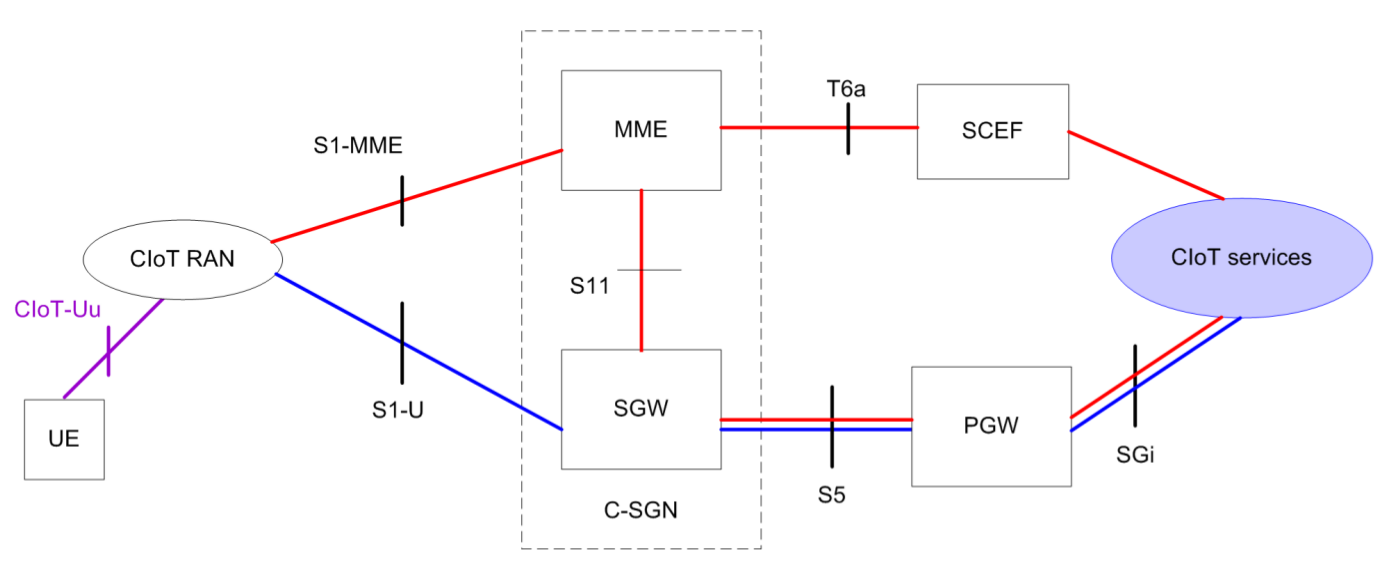
\includegraphics[width=\textwidth]{figures/NB-Network.png}
\definecolor{purple}{HTML}{7030A0}
\usetikzlibrary{arrows}
\definecolor{red}{HTML}{FF0000}
\definecolor{blue}{HTML}{00B0F0}

\resizebox{\textwidth}{!}{
\begin{tikzpicture}[scale=0.5]


\draw  (-14,5) rectangle (-10,3);
\node at (-12,4) {Device};
\draw  (-4,14) rectangle (2,-8);
\draw  (6,9) rectangle (10,7);
\draw  (6,1) rectangle (10,-1);
\node at (-1,-7) {\acrshort{CIoT} \acrshort{RAN}};
\node at (8,8) {\acrshort{MME}};
\node at (8,0) {\acrshort{SGW}};
 




\draw  (14,1) rectangle (18,-1);
\draw  (14,13) rectangle (18,11);
\draw  (25,6) ellipse (3 and 2);
\node at (16,12) {\acrshort{SCEF}};

\node at (16,0) {\acrshort{PGW}};
\node at (25,6) {\acrshort{CIoT} Services};

\draw  (-3,13) rectangle (1,11);
\draw  (-3,5) rectangle (1,3);
\draw  (-3,-3) rectangle (1,-5);
\node at (-1,12) {\acrshort{eNB}};
\node at (-1,4) {\acrshort{eNB}};
\node at (-1,-4) {\acrshort{eNB}};

\draw (6,18) -- (6,15); 
\draw (10,15) -- (10,18);
\draw  (8,18) ellipse (2 and 0.5);
\node at (8,15.4) {\acrshort{HSS}};
\draw (6,15) arc (-120:-60:4);

\draw (14,8.6) -- (14,5.6);
\draw (18,5.6) -- (18,8.6);
\draw  (16,8.6) ellipse (2 and 0.5);
\node at (16,6) {\acrshort{PCRF}};
\draw (14,5.6) arc (-120:-60:4);
\node (v27) at (16,5) {};


\node (v2) at (-7,4) {\acrshort{CIoT}-Uu};
\node (v1) at (-10,4) {};
\node (v3) at (-4,4) {};
\draw [draw=purple, arrows={triangle 45-},fill=purple] (v1) edge (v2);
\draw [draw=purple, arrows={-triangle 45},fill=purple] (v2) edge (v3);

\node (v5) at (-1,8) {X2};
\node (v8) at (-1,0) {X2};
\node (v4) at (-1,11) {};
\node (v6) at (-1,5) {};
\node (v7) at (-1,3) {};
\node (v9) at (-1,-3) {};
\draw [draw=red, arrows={triangle 45-},fill=red] (v4) edge (v5);
\draw [draw=red, arrows={-triangle 45},fill=red] (v5) edge (v6);
\draw [draw=red, arrows={triangle 45-},fill=red] (v7) edge (v8);
\draw [draw=red, arrows={-triangle 45},fill=red] (v8) edge (v9);
\node (v10) at (2,4) {};
\node (v14) at (6,0) {};
\node (v12) at (6,8) {};
\node (v18) at (8,7) {};
\node (v20) at (8,1) {};
\node (v17) at (8,9) {};
\node (v15) at (8,14.4) {};
\node (v21) at (10,8) {};
\node (v23) at (14,12) {};

\node (v24) at (10,0) {};
\node (v26) at (14,0) {};

\node (v33) at (18,0) {};
\node (v32) at (22,6) {};
\node (v30) at (18,12) {};
\node (v29) at (16,1) {};

\node (v11) at (4,6) {S1-\acrshort{MME}};
\node (v13) at (4,2) {S1-U};
\node (v19) at (8,4) {S11};
\node (v16) at (8,12) {S6a};
\node (v22) at (12,10) {T6a};
\node (v25) at (12,0) {S5};
\node (v28) at (16,3) {S7};
%\node (v31) at (20,9) {};
\node (v34) at (20,3) {SGi};

\draw [draw=red, arrows={triangle 45-},fill=red]  (v10) edge (v11);
\draw [draw=red, arrows={-triangle 45},fill=red]  (v11) edge (v12);
\draw [draw=blue, arrows={triangle 45-},fill=blue]  (v10) edge (v13);
\draw [draw=blue, arrows={-triangle 45},fill=blue]  (v13) edge (v14);


\draw [draw=red, arrows={triangle 45-},fill=red]   (v15) edge (v16);
\draw [draw=red, arrows={-triangle 45},fill=red]  (v16) edge (v17);
\draw [draw=red, arrows={triangle 45-},fill=red]  (v18) edge (v19);
\draw [draw=red, arrows={-triangle 45},fill=red]  (v19) edge (v20);
\draw [draw=red, arrows={triangle 45-},fill=red]  (v21) edge (v22);
\draw [draw=red, arrows={-triangle 45},fill=red]  (v22) edge (v23);
\draw [draw=purple, arrows={triangle 45-},fill=purple]  (v24) edge (v25);
\draw [draw=purple, arrows={-triangle 45},fill=purple]  (v25) edge (v26);
\draw [draw=red, arrows={triangle 45-},fill=red]  (v27) edge (v28);
\draw [draw=red, arrows={-triangle 45},fill=red]  (v28) edge (v29);
\draw [draw=red, arrows={triangle 45-triangle 45},fill=red]  (v30) edge (v32);
%\draw [draw=red, arrows={-triangle 45},fill=red]  (v31) edge (v32);
\draw [draw=purple, arrows={triangle 45-},fill=purple]  (v33) edge (v34);
\draw [draw=purple, arrows={-triangle 45},fill=purple]  (v34) edge (v32);
\end{tikzpicture}
}
\caption{Overview over the network blocks and interfaces between blocks in \gls{NB-IoT}. Blue lines are user plane \gls{CIoT} \gls{EPS} optimization, the red lines are control plane \gls{CIoT} \gls{EPS} optimization plane and the purple lines are both \citep{NB_slide}}
\label{fig:network_structure}
\end{figure}


\textbf{\gls{UE}}\\
The \gls{UE} is the smart meters or other products as mentioned, they do not need to transmit a lot of data and it is not critical that it arrives within a certain time frame. They do however require a long battery life time. The problem comes in terms of placement, because many of these devices might be placed in basement like environment which means an increased path loss. The system needs to be able to operate with a \gls{MCL} of 164 dB \citep{REL-13}. As in previous systems the \gls{USIM} is located on the \gls{UE} for authentication purpose \citep[ch. 3]{book_LTE_for_UMTS}.

\textbf{\gls{CIoT} \gls{RAN}}\\
The \gls{CIoT} \gls{RAN} is the base stations, the most typically used is the \gls{eNB} base station. All radio communication terminates at this node. Any \gls{UE} that wish to use an external service, interfaces with the \gls{eNB} \citep{book_LTE_for_UMTS}. The \gls{eNB} interfaces with both the \gls{MME} and the \gls{SGW}. On the control plane (connection to the \gls{MME}) the \gls{eNB} is in charge of \gls{RRM}, i.e. allocating radio resources in the user plane to the individual \gls{UE} based on \gls{QoS} measures. 

\textbf{\gls{MME}}\\
The \gls{MME} takes care of mobility issues, it also keep track of where in the network different \gls{UE}s are connected \citepalias{3GPP_MME_spec}. Another very important function of the \gls{MME} is to handle authentication of \gls{UE}s and setting up security for the data bearers. The \gls{MME} might be connected to multiple \gls{UE}s, however a \gls{UE} may only be connected to a single \gls{MME} \citep[ch. 3]{book_LTE_for_UMTS}. In \gls{NB-IoT} handovers are omitted and the only way to change cell is by releasing the existing connection \citep{REL-13}. The \gls{MME} also handles paging procedures \citep{NB-IoT_Book}.

\textbf{\gls{HSS}}\\
The \gls{HSS} stores the identity of the users, which the \gls{MME} uses for authentication purposes. It records the location of the \gls{UE} in level of visited network control nodes  such as \gls{MME}, it also keep track of which networks the user is allowed to roam to \citep[ch. 3]{book_LTE_for_UMTS}.

\textbf{\gls{SCEF}}\\
The \gls{SCEF} is a multi functional unit, task it handles include: device trigger delivery, sponsored data, \gls{UE} reachability, \gls{3GPP} network issues, \gls{QoS} for a \gls{UE} session etc. Many of these functionalities are meant for normal \gls{LTE} use. Uses meant for \gls{NB-IoT} include \gls{UE} reachability which enables the application layer to be informed when a \gls{UE} reconnects to the network i.e. after an \gls{eDRX} or after \gls{PSM}. Another functionality it handles is \gls{NIDD}, which enables \gls{UE}s with small data volumes to send it data with less overhead and thereby have a longer battery life time \citepalias{3GPP_SCEF_primer}.

\textbf{\gls{SGW}}\\
The \gls{SGW} is primarily a routing unit. It interfaces with the \gls{eNB}, the \gls{MME} and the \gls{PGW}. When the \gls{UE} transmit data it is send to the \gls{eNB} and then routed via the \gls{SGW} to the \gls{PGW} before reaching the providers. The \gls{SGW} typically serve a particular geographic area with several \gls{eNB}s, likewise could the \gls{MME} also serve a particular geographic area. In \gls{LTE} this was the last node in the network that could change during a connected state meaning that all \gls{SGW}s needs to be connected to all \gls{PGW}s \citep[ch. 3]{book_LTE_for_UMTS}. This is however not equally important in \gls{NB-IoT} as no handovers are expected \citep{REL-13}. During connected state the \gls{SGW} works as a relay, however in idle mode the resources are released in the \gls{eNB} and the data path terminates at the \gls{SGW} it then stores the data from the \gls{PGW} and request the \gls{MME} to initiate paging of the \gls{UE} \citep[ch. 3]{book_LTE_for_UMTS}.

\textbf{\gls{PGW}}\\
The \gls{PGW} is the edge of the \gls{EPS}. It function as the point of attachment for the \gls{UE}s \gls{IP} traffic. The \gls{IP}-address of the \gls{UE} is allocated during the connection procedure when the \gls{UE} request a \gls{PDN} connection and during any subsequent \gls{PDN} connection request. It is the \gls{PGW} that performs the \gls{DHCP} functionality \citep[ch. 3]{book_LTE_for_UMTS}. The \gls{PGW} handle interfaces to external CIoT services on a higher level.

\textbf{\gls{PCRF}}\\
The \gls{PCRF} is a server that makes decision on how to handle services provided for the \gls{UE} in terms of \gls{QoS}. It informs the \gls{PGW} and if applicable the \gls{SGW} about appropriate bearer policy can be set up. A default bearer is set up during connection request and either the \gls{UE} or the service domain can request additional bearers which is handled by the \gls{PCRF} \citep[ch. 3]{book_LTE_for_UMTS}.

\textbf{\gls{CIoT} services}\\
The \gls{CIoT} services are typically storage functionalities, but could be control algorithms or other services needed for specific products. 

%connections across the network

\section{Protocol Layers}

The following section is focused on the communication protocol in the \gls{CIoT}-Uu interface. It consist of the following six layers:
\begin{itemize}
	\item \gls{NAS} layer
	\item \gls{RRC} layer
	\item \gls{PDCP} layer
	\item \gls{RLC} layer
	\item \gls{MAC} layer
	\item \gls{PHY} layer
\end{itemize}

The purpose and functionalities of these layers are explained in the following.

\subsection{NAS}
The \gls{NAS} layer is the top layer in the control plane. It signals directly between the device and the \gls{MME} \citep[ch. 3]{book_LTE_for_UMTS}. There are two protocols in the \gls{NAS} layer, the \gls{EMM} and the \gls{ESM}. The \gls{EMM} handles re-activation from idle mode: the device initiated case is called service request, the network initiated case is called paging. The \gls{EMM} protocol is used for handling attachment and detachment from the system when the device is in idle mode. In connected mode lower layer protocols handles this instead \citep[ch. 3]{book_LTE_for_UMTS}. In the NB-IoT protocol, a functionality has been implemented, to transmit data directly through the NAS layer \citep{REL-13}. 

\subsection{RRC} \label{sec:RRC}
The \gls{RRC} layer of the protocol is a strictly control plane layer. The functionalities provided by the \gls{RRC} are \citep[ch. 6.6]{book_LTE_for_UMTS}:

\begin{itemize}
	\item Broadcast of system information
	\item Paging
	\item Establishment, maintenance and release of an \gls{RRC} connection between device and the \gls{eNB}
	\item Security functions, including key management
	\item Establishment, maintenance and release of point to point radio bearers
	\item Device measurement reporting and control of the reporting
	%\item Handover
	\item Device cell selection and reselections 
%	\item Context transfer between \gls{eNB}s
	\item Device capability transfer
	\item Generic protocol error handling
	\item Support of self-configuration and self-optimization
\end{itemize}

One of the biggest changes from \gls{LTE} to \gls{NB-IoT} is the focus on reducing power consumption. Therefore a new state has been introduced compared to the \gls{LTE} system, which can be seen on \autoref{fig:UE-states}.

\tikzsetnextfilename{state-diagram}
\begin{figure}[H]
\centering
\usetikzlibrary{arrows}
%\usetikzlibrary{shapes.multipart}
\renewcommand{\arraystretch}{0.8}
\resizebox{\textwidth}{!}{
\begin{tikzpicture}[scale=0.5]

\draw  (-26,28) ellipse (3 and 2);
\node at (-26,28) {Start up};

\draw  (-17,28) ellipse (3 and 2);
\node at (-17,28) {Idle state};

\draw  (-24.5,11) ellipse (3 and 2);
%\node at (-17,15) {\acrshort{PSM}};
\node at (-24.5,11) {PSM};

\draw  (-10,19.5) rectangle (-4,16.5);
\node at (-7,18) {\begin{tabular}{c} Resume RRC \\ connection \end{tabular}};

\draw  (-10,26.5) rectangle (-4,23.5);
\node at (-7,25) {\begin{tabular}{c} Establish RRC \\ connection\end{tabular}};

\draw  (-10,13.5) rectangle (-4,10.5);
\node at (-7,12) {\begin{tabular}{c} Suspend RRC \\ connection\end{tabular}};

\draw  (-10,32.5) rectangle (-4,29.5);
\node at (-7,31) {\begin{tabular}{c} Release RRC \\ connection\end{tabular}};

\draw  (4,21.5) ellipse (3 and 2);
\node at (4,21.5) {Connected state};

\draw  (-17,15) ellipse (3 and 2);
\node at (-17,15) {\begin{tabular}{c} Idle state \\ (with AS)\end{tabular}};
\node (v22) at (-20,15) {};
\node (v23) at (-14,15) {};

\draw  (-24.5,19) ellipse (3 and 2);
\node at (-24.5,19) {eDRX};
\node (v25) at (-19,16.5) {};
\node (v26) at (-22,18) {};
\node (v27) at (-22.5,17.5) {};
\node (v28) at (-19.5,16) {};
\node[rotate=27] at (-21.5,14) {\begin{tabular}{c} PSM\\ command\end{tabular}};
\node[rotate=27] at (-20.25,12.25) {Timer};




\node (v1) at (-23,28) {};
\node (v2) at (-20,28) {};
\node (v3) at (-14,28) {};
\node (v4) at (-10,25) {};
\node (v5) at (-4,25) {};
\node (v6) at (1,21.5) {};
\node (v7) at (-4,12) {};
\node (v8) at (-4,31) {};
\node (v9) at (-4,18) {};
\node (v10) at (-10,18) {};
\node (v11) at (-10,12) {};
\node (v12) at (-10,31) {};
\node (v13) at (-7,19.5) {};
\node (v14) at (-7,23.5) {};
\node (v15) at (-19.5,14) {};
\node (v16) at (-22.5,12.5) {};
\node (v17) at (-22,12) {};
\node (v18) at (-19,13.5) {};



\draw [arrows={- triangle 45}] (v1) edge (v2);
\draw [arrows={- triangle 45}] (v23) edge (v10);
\draw [arrows={- triangle 45}] (v3) edge (v4);
%\draw [arrows={triangle 45-}]  (v4) edge ($(midpoint)+(0,0)$);

\draw [arrows={- triangle 45}] (v11) edge (v23);
\draw [arrows={- triangle 45}] (v12) edge (v3);
\draw [arrows={- triangle 45}] (v13) edge (v14);
\draw [arrows={- triangle 45}] (v9) edge (v6);
\draw [arrows={- triangle 45}] (v5) edge (v6);
\draw [arrows={- triangle 45}] (v6) edge (v7);
\draw [arrows={- triangle 45}] (v6) edge (v8);
\draw [arrows={- triangle 45}] (v15) edge (v16);
\draw [arrows={- triangle 45}]  (v17) edge (v18);
\draw [arrows={- triangle 45}] (v25) edge (v26);
\draw [arrows={- triangle 45}]  (v27) edge (v28);


\node at (-21.75,28.5) {Sync};
\node[rotate=-27] at (-20,18) {\begin{tabular}{c} eDRX \\ command\end{tabular}};
\node[rotate=-27] at (-21.25,16.25) {Timer};
\node[rotate=39] at (-12.2,30) {Ok};
\node[rotate=39] at (-12.2,17.1) {Data/paging};
\node[rotate=-39] at (-12.2,13) {Ok};
\node[rotate=-39] at (-12.4,26.1) {Data};
\node[rotate=-35] at (-2,24.2) {Complete};
\node[rotate=35] at (-2,20) {Complete};
\node[rotate=62] at (-0.8,16.8) {No more data};
\node[rotate=-62] at (-0.8,26.2) {No more data};
\node[rotate=90] at (-7.5,21.5) {Reject};


\end{tikzpicture}
}
\caption{State diagram with transition options for a device.}
\label{fig:UE-states}
\end{figure}


With this new structure comes a greater focus on \gls{RRC} connection resume, which is very advantageous with regards to power consumption, as it allows the device to suspend its connection and save its \gls{AS}, when going into idle mode.

This enables the device to request a connection resume, where it uses its previous \gls{AS} to reduces the overhead considerably. This can also be seen from \autoref{tab:signaling_comparison} where a comparison between the different procedures is shown. 

\begin{table}[H]
\centering
\resizebox{\textwidth}{!}{
\begin{tabular}{|p{2.5cm}|p{4cm}|p{4cm}|p{4cm}|} \hline
\rowcolor{gray!50}\textbf{Direction} & \raggedright\arraybackslash\textbf{Legacy Service Request Procedure}	& \raggedright\arraybackslash\textbf{\gls{RRC} Connection Resume} & \textbf{Control Plane Data Transfer}  \\\hline
UL	& \multicolumn{3}{c|}{Preamble} \\\hline
\rowcolor{gray!10}DL	& \multicolumn{3}{c|}{\gls{RAR}} \\\hline
UL	& \raggedright\arraybackslash \gls{RRC} Connection Request						& \raggedright\arraybackslash \gls{RRC} Connection Resume Request	& \raggedright\arraybackslash \gls{RRC} Connection Request \\\hline
\rowcolor{gray!10}DL	& \raggedright\arraybackslash \gls{RRC} Connection Setup						& \raggedright\arraybackslash \gls{RRC} Connection Resume 			& \raggedright\arraybackslash \gls{RRC} Connection Setup   \\\hline
UL	& \raggedright\arraybackslash \gls{RRC} Connection Request Complete 			& \raggedright\arraybackslash \gls{RRC} Connection Resume Complete & \raggedright\arraybackslash \gls{RRC} Connection Complete  \\\hline
\rowcolor{gray!10}DL	& \raggedright\arraybackslash Security Mode Command 							& - & -  \\\hline
UL	& \raggedright\arraybackslash Security Mode Complete 							& - & -  \\\hline
\rowcolor{gray!10}DL	& \raggedright\arraybackslash \gls{RRC} Connection Reconfiguration 			& - & -  \\\hline
UL	& \raggedright\arraybackslash \gls{RRC} Connection Reconfiguration Complete 	& - & -  \\\hline
\raggedright\arraybackslash \textbf{Total number of messages} 					& \textbf{9} & \textbf{5} & \textbf{5} \\\hline
\end{tabular}
}
\caption{Signaling comparison between different methods \citep{REL-13}.}
\label{tab:signaling_comparison}
\end{table}

\textbf{\Gls{SRB}}\\
The \gls{RRC} sets up three different \gls{SRB}s, which are used to carry \gls{RRC} and \gls{NAS} messages. \gls{SRB}0 is used for \gls{CCCH} during \gls{RRC} connection setup or during link failure. Messages carried here include \gls{RRC} connection request, \gls{RRC} connection setup, \gls{RRC} connection reject, \gls{RRC} connection reestablishment request, \gls{RRC} connection reestablishment and \gls{RRC} connection reestablishment reject. \gls{SRB}1 is used when a \gls{RRC} connection is established. It is used to transfer both \gls{RRC} messages, using \gls{DCCH}, and \gls{NAS} messages until security is established. Once security is established, the \gls{NAS} messages is carried on \gls{SRB}2, which has a lower priority. \citep[ch. 6.6]{book_LTE_for_UMTS} 


\textbf{\gls{SIB}s}\\
Before the device attempts to access the system, it needs a lot of information about the system, which is carried in the \gls{SIB}s. For \gls{NB-IoT} there are eight different \gls{SIB}s messages. A list of the information carried in the different \gls{SIB}s can be seen in \autoref{tab:NB-SIB}. The \gls{RRC} takes care of updating these messages and paging the devices if changes occurs.

\begin{table}[H]
\centering
\begin{tabular}{|p{3cm}|p{8cm}|p{3cm}|}\hline
\textbf{Name}		& \textbf{Information}																	& \textbf{Update rate}	\\\hline
\raggedright\arraybackslash\gls{MIB-NB}		& Essential information required to receive further system information 					& 640 ms				\\\hline
\raggedright\arraybackslash\gls{NB-SIB}1		& Cell access and selection and the other SIBs scheduling 										& 40.96 s 				\\\hline
\gls{NB-SIB}2		& Radio resource configuration information 												& NA 					\\\hline
\gls{NB-SIB}3		& Cell re-selection information for intra-frequency, inter-frequency 					& NA 					\\\hline
\gls{NB-SIB}4		& Neighboring cell related information relevant for intra-frequency cell re-selection 	& NA 					\\\hline
\gls{NB-SIB}5		& Neighboring cell related information relevant for inter-frequency cell re-selection 	& NA 					\\\hline
\gls{NB-SIB}14		& Access barring parameters 															& Fast 					\\\hline
\gls{NB-SIB}16		& Information related to GPS time and Coordinated Universal Time (UTC) 					& Fast 					\\\hline
\end{tabular}
\caption{List of different \gls{SIB} messages and the information carried within \citep{whitepaper,REL-13}.}
\label{tab:NB-SIB}
\end{table}

\textbf{Paging} \\
Paging serves two main functions: the first is to notify a device in \gls{RRC} idle state to set up a \gls{RRC} connection to handle incoming data and the second is to inform the devices, both in \gls{RRC} idle and \gls{RRC} connected state, that the system information has changed. \citep[ch. 7]{NB-IoT_Book}

\textbf{Establishment, Maintenance and Release of \gls{RRC} Connection} \\
When an \gls{RRC} connection setup is requested, the \gls{eNB} has the option to reject it with a wait timer, if the network is overloaded. The \gls{RRC} can set the access barring parameter appropriately depending on the traffic load. In the \gls{RRC} connection request message, the device can trasmit its \gls{S-TMSI} if it possess a valid version, else it will transmit a 40 bit random value. Five different establishment causes has been defined: emergency, high-priority access, mobility-terminated access, mobile-originated signaling and mobile-originated data. In \gls{NB-SIB}1 there exists at most six different \gls{PLMN} identities, where the device selects one and reports it in the  \gls{RRC} connection setup complete message, along with any \gls{MME} the device might already be registered to. The \gls{eNB} then finds the \gls{MME} and starts the S1 connection setup. When a connection setup is successful the device moves to the \gls{RRC} connected state. \citep[ch. 6.6]{book_LTE_for_UMTS}

%\todo{should we put detailed connection options in here, should we go in detail with further RRC functions and what about radio bearers}

%\textbf{\gls{UE} Measurement Reporting and Control of the Reporting} \\


%%% pic for rrc connection resume
%\begin{figure}[H]
%\centering
%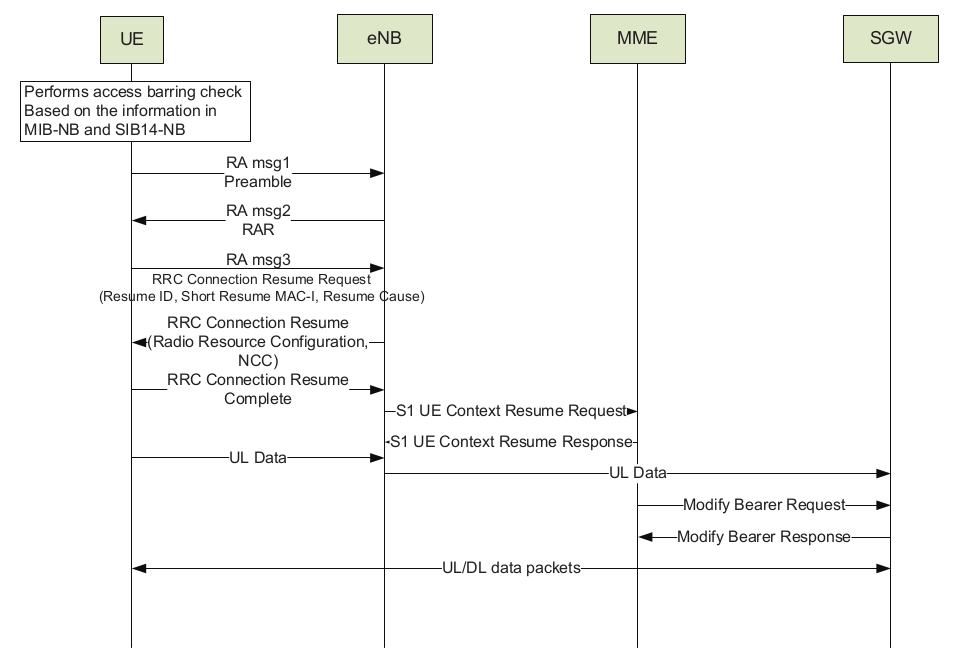
\includegraphics[width=\textwidth]{figures/RRC_resume.png}
%\caption{Signaling procedure for a \gls{RRC} resume request}
%\label{fig:RRC_resume}
%\end{figure}

\subsection{PDCP}
The \gls{PDCP} layer is just below the \gls{RRC}, where it handles both control functions as well as device data. The key function of the \gls{PDCP} include \citep[ch. 6.5]{book_LTE_for_UMTS}:
\begin{itemize}
	\item Header compression and decompression of \gls{IP} packets. This is an important function especially for small data packets, as the overhead could become quite significant
	\item Ciphering and deciphering of both user plane and most of control plane data
	\item Integrity protection and verification to ensure control data comes from the correct source
\end{itemize}

The \gls{PDCP} gets \gls{PDCP} \gls{SDU}s from the \gls{RRC} and \gls{NAS} layer. 

\tikzsetnextfilename{PDCP_data_flow}
\begin{figure}[H]
\centering
\resizebox{0.8\textwidth}{!}{
\begin{tikzpicture}[scale=.5]


\node (v2) at (-0.5,8) {NAS};
\draw  (-1,7) rectangle (-14,-9);
\draw  (0,7) rectangle (13,-9);
\node[anchor=west] at (-14,6) {Transmitting side};
\node[anchor=east] at (13,6) {Receiving side};

\draw  (-10,5) rectangle (-5,3);
\node at (-7.5,4) {\begin{tabular}{c} Sequence \\[-0.9em] numbering \end{tabular}};
\draw  (-13,1) rectangle (-8,-1);
\node at (-10.5,0) {\begin{tabular}{c} Integrity \\[-0.9em] protection \end{tabular}};
\draw  (-7,1) rectangle (-2,-1);
\node at (-4.5,0) {\begin{tabular}{c} Header \\[-0.9em] compression \end{tabular}};
\draw  (-11,-3) rectangle (-4,-5);
\node at (-7.5,-4) {Ciphering};
\draw  (-13,-6) rectangle (-7,-8) node (v1) {};
\draw  (v1) rectangle (-2,-6);
\node at (-10,-7) {PDCP header};
\node at (-4.5,-7) {Data field};
\node (v12) at (-7,-10) {RLC};

\node (v3) at (-7.5,5) {};
\node (v4) at (-7.5,3) {};
\node (v5) at (-10.5,1) {};
\node (v6) at (-4.5,1) {};
\node (v9) at (-4.5,-1) {};
\node (v7) at (-10.5,-1) {};
\node (v8) at (-7.5,-3) {};
\node (v10) at (-7,-5) {};
\node (v11) at (-4.5,-6) {};
\draw  [- triangle 45] (v2) -- (-7.5,5);
\draw  [- triangle 45] (-7.5,3) -- (-10.5,1);
\draw  [- triangle 45] (-7.5,3) -- (-4.5,1);
\draw  [- triangle 45] (-10.5,-1) -- (-7.5,-3);
\draw  [- triangle 45] (-4.5,-1) -- (-7.5,-3);
\draw  [- triangle 45] (-7.5,-5) -- (-4.5,-6);
\draw  [- triangle 45] (-7,-8) -- (v12);
\node[anchor=east] at (-9.2,2) {\begin{tabular}{c} \textbf{Control} \\[-0.9em] \textbf{Plane} \end{tabular}};
\node[anchor=west] at (-5.4,2) {\begin{tabular}{c} \textbf{User} \\[-0.9em] \textbf{Plane} \end{tabular}};

\draw  (12,5) rectangle (7,3);
\node at (9.5,4) {Reordeing};
\draw  (6,1) rectangle (1,-1);
\node at (3.5,0) {\begin{tabular}{c} Integrity \\[-0.9em] protection \end{tabular}};
\draw  (12,1) rectangle (7,-1);
\node at (9.5,0) {\begin{tabular}{c} Header \\[-0.9em] decompression \end{tabular}};
\draw  (10,-3) rectangle (3,-5);
\node at (6.5,-4) {Deciphering};
\draw  (12,-6) rectangle (7,-8) node (v1) {};
\draw  (v1) rectangle (1,-6);
\node at (4,-7) {PDCP header};
\node at (9.5,-7) {Data field};

\node (v3) at (-7.5,5) {};
\node (v4) at (-7.5,3) {};
\node (v5) at (3.5,1) {};
\node (v6) at (9.5,1) {};
\node (v9) at (9.5,-1) {};
\node (v7) at (3.5,-1) {};
\node (v8) at (6.5,-3) {};
\node (v10) at (6,-5) {};
\node (v11) at (9.5,-6) {};
\node (v14) at (9.5,3) {};
\node (v15) at (7,4) {};
\node (v13) at (7,-10) {RLC};

\draw [- triangle 45] (v13) -- (7,-8);
\draw [- triangle 45] (9.5,-6) -- (6.5,-5);
\draw [- triangle 45] (6.5,-3) -- (3.5,-1);
\draw [- triangle 45] (6.5,-3) -- (9.5,-1);
\draw [- triangle 45] (9.5,1) -- (9.5,3);
\draw [- triangle 45] (7,4) -- (v2);
\draw [arrows={triangle 45 - triangle 45}] (3.5,1) -- (v2);
\node[anchor=east] at (4.3,-2) {\begin{tabular}{c} \textbf{Control} \\[-0.9em] \textbf{Plane} \end{tabular}};
\node[anchor=west] at (8.5,-2) {\begin{tabular}{c} \textbf{User} \\[-0.9em] \textbf{Plane} \end{tabular}};

\end{tikzpicture}}
\caption{\gls{PDCP} layer operation with associated \gls{PDCP} \gls{SDU} \citep[fig. 6.12]{book_LTE_for_UMTS}.}
\label{fig:PDCP_operation}
\end{figure}

As can be seen on \autoref{fig:PDCP_operation}, before forwarding the data to the \gls{RLC} layer, it is first numbered and then either integrity protection or header compression is applied, depending on whether or not it is control plane data or user plane data. It is then ciphered and forwarded. When the \gls{PDCP} receive data from the \gls{RLC} layer, it is first deciphered and again depending on whether it is control or user plane data, is it integrity protected or header decompressed and reordered, before forwarding it to the \gls{NAS}. \citep[ch. 6.5]{book_LTE_for_UMTS}  

%The \gls{PDCP} layer also handles alot during handovers, however as handovers is out of the scope for \gls{NB-IoT} these functionalities are obsolete. 

\subsection{RLC}

The \gls{RLC} layer has three basic functionalities \cite[ch. 6.4]{book_LTE_for_UMTS}:

\begin{itemize}
	\item To transfer \gls{PDU}s from higher layers i.e. \gls{RRC}, \gls{NAS} or \gls{PDCP}
	\item Depending on the \gls{RLC} mode used, error correction with \gls{ARQ}, concatenation/segmentation, in-sequence delivery and duplicate detection may occur
	\item Protocol error handling to detect and recover from protocol error states caused by e.g. signaling errors
\end{itemize}

\captionsetup{belowskip=0em}
\begin{minipage}[H]{0.48\textwidth}
\tikzsetnextfilename{RLC_UM-SAP}
\begin{figure}[H]
\centering
\resizebox{\textwidth}{!}{
\begin{tikzpicture}[scale=.5]

\draw  (-1,8.5) rectangle (-14,-8);
\draw  (0,8.5) rectangle (13,-8);

\node (v1) at (-6,6) {Transmission Buffer};
\draw  (v1) ellipse (4 and 1);
\draw (-10,5.5) arc (180:360:4 and 1);
\draw (-10,5) arc (180:360:4 and 1);
\draw (-10,2) arc (180:360:4 and 1);
\node (v2) at (-10,6) {};
\node (v4) at (-2,6) {};
\node (v3) at (-10,1.7) {};
\node (v5) at (-2,1.7) {};
\draw  (v2) ++(0,0) edge (v3);
\draw  (v4)  ++(0,0) edge (v5);

\draw  (-9,-1) rectangle (-3,-3);
\node at (-6,-2) {\begin{tabular}{c} Segmentation/ \\[-0.9em] Concatenation\end{tabular}};
\draw  (-13,-5) rectangle (-8,-7) node (v6) {};
\draw  (v6) rectangle (-3,-5);
\node at (-10.5,-6) {UM Header};
\node at (-5.5,-6) {Data Field};



\node (v10) at (7,2) {Receiving Buffer};
\draw  (v10) ellipse (4 and 1);
\draw (3,1.5) arc (180:360:4 and 1);
\draw (3,1) arc (180:360:4 and 1);
\draw (3,-2) arc (180:360:4 and 1);
\node (v20) at (3,2) {};
\node (v40) at (11,2) {};
\node (v30) at (3,-2.3) {};
\node (v50) at (11,-2.3) {};
\draw  (v20) ++(0,0) edge (v30);
\draw  (v40)  ++(0,0) edge (v50);


\draw  (4.5,7) rectangle (9.5,5);
\draw  (1,-5) rectangle (6,-7) node (v7) {};
\draw  (v7) rectangle (11,-5);
\node at (7,6) {Reasembly};
\node at (7,-1.5) {\& HARQ Reordering};
\node at (3.5,-6) {UM Header};
\node at (8.5,-6) {Data Field};

\node (v15) at (-8,-9) {Logic Channels};
\node (v16) at (6,-9) {Logic Channels};
\node (v14) at (-5.5,-5) {};
\node (v13) at (-6,-3) {};
\node (v11) at (-6,1) {};
\node (v9) at (-6,7) {};
\node (v8) at (-1,9.5) {UM-Service Access Point};
\node (v22) at (7,7) {};
\node (v21) at (7,5) {};
\node (v19) at (7,3) {};
\node (v18) at (7,-3) {};
\node (v17) at (8.5,-5) {};
\node (v12) at (-6,-1) {};

\draw [arrows={ - triangle 45}] (v8) edge (v9);
\draw [arrows={ - triangle 45}] (v11) edge (v12);
\draw [arrows={ - triangle 45}] (v13) edge (v14);
\draw [arrows={ - triangle 45}] (v6) edge (v15);
\draw [arrows={ - triangle 45}] (v16) edge (v7);
\draw [arrows={ - triangle 45}] (v17) edge (v18);
\draw [arrows={ - triangle 45}] (v19) edge (v21);
\draw [arrows={ - triangle 45}] (v22) edge (v8);
\node [anchor=west] at (-14,7.75) {Transmitting Side};
\node [anchor=east] at (13,7.75) {Receiving Side};
\end{tikzpicture}}
\caption{\gls{RLC} \gls{UM} operation \citep[ch. 6.4]{book_LTE_for_UMTS}.}
\label{fig:RLC_AM/UM_operation2}
\end{figure}
\end{minipage}
\begin{minipage}[H]{0.48\textwidth}
\begin{figure}[H]
\tikzsetnextfilename{RLC_AM-SAP}
\centering
\resizebox{\textwidth}{!}{
\begin{tikzpicture}[scale=.5]

\draw  (-1,9) rectangle (-17,-8);
\draw  (0,9) rectangle (13,-8);

\node (v1) at (-12,6) {Transmission Buffer};
\draw  (v1) ellipse (4 and 1);
\draw (-16,5.5) arc (180:360:4 and 1);
\draw (-16,5) arc (180:360:4 and 1);
\draw (-16,2) arc (180:360:4 and 1);
\node (v2) at (-16,6) {};
\node (v4) at (-8,6) {};
\node (v3) at (-16,1.7) {};
\node (v5) at (-8,1.7) {};
\draw  (v2) ++(0,0) edge (v3);
\draw  (v4)  ++(0,0) edge (v5);

\draw  (-9,-1) rectangle (-3,-3);
\node at (-6,-2) {\begin{tabular}{c} Segmentation/ \\[-0.9em] Concatenation\end{tabular}};
\draw  (-15,-5) rectangle (-10,-7) node (v6) {};
\draw  (v6) rectangle (-5,-5);
\node at (-12.5,-6) {AM Header};
\node at (-7.5,-6) {Data Field};



\node (v10) at (7,2) {Receiving Buffer};
\draw  (v10) ellipse (4 and 1);
\draw (3,1.5) arc (180:360:4 and 1);
\draw (3,1) arc (180:360:4 and 1);
\draw (3,-2) node (v23) {} arc (180:360:4 and 1);
\node (v20) at (3,2) {};
\node (v40) at (11,2) {};
\node (v30) at (3,-2.3) {};
\node (v50) at (11,-2.3) {};
\draw  (v20) ++(0,0) edge (v30);
\draw  (v40)  ++(0,0) edge (v50);


\draw  (4.5,7) rectangle (9.5,5);
\draw  (1,-5) rectangle (6,-7) node (v7) {};
\draw  (v7) rectangle (11,-5);
\node at (7,6) {Reasembly};
\node at (7,-1.5) {};
\node at (3.5,-6) {AM Header};
\node at (8.5,-6) {Data Field};

\node (v15) at (-10,-9) {Logic Channels};
\node (v16) at (6,-9) {Logic Channels};
\node (v14) at (-7.5,-5) {};
\node (v13) at (-6,-3) {};
\node (v11) at (-12,1) {};
\node (v9) at (-12,7) {};
\node (v8) at (-0.5,10) {AM-Service Access Point};
\node (v22) at (7,7) {};
\node (v21) at (7,5) {};
\node (v19) at (7,3) {};
\node (v18) at (7,-3) {};
\node (v17) at (8.5,-5) {};
\node (v12) at (-6,-1) {};

\draw [arrows={ - triangle 45}] (v8) -- (-12,7);
\draw [arrows={ - triangle 45}] (-12,1) -- (-6,-1);
\draw [arrows={ - triangle 45}] (-6,-3) -- (-7.5,-5);
\draw [arrows={ - triangle 45}] (-10,-7) -- (v15);
\draw [arrows={ - triangle 45}] (v16) -- (6,-7);
\draw [arrows={ - triangle 45}] (8.5,-5) -- (7,-3);
\draw [arrows={ - triangle 45}] (7,3) -- (7,5);
\draw [arrows={ - triangle 45}] (7,7) -- (v8);
\node [anchor=west] at (-17,8) {Transmitting side};
\node [anchor=east] at (13,8) {Receiving side};
\draw  (-10,-1) rectangle (-16,-3);
\node at (-13,-2) {\begin{tabular}{c} Retransmission \\[-0.9em] Buffer\end{tabular}};
\draw  (-7,4) rectangle (-2,2) node (v24) {};
\node at (-4.5,3) {Control};
\draw [arrows={ - triangle 45}] (3,-2) -- (-2,2);
\node [anchor=west] at (0,1) {Status};
\node (v25) at (-10.2,-2) {};
\node (v26) at (-8.8,-2) {};
\node (v27) at (-13.5,-3) {};
\draw [arrows={ - triangle 45}] (-10,-2) -- (-9,-2);
\draw [arrows={ - triangle 45}] (-13.5,-3) -- (-7.5,-5);
\end{tikzpicture}}
\caption{\gls{RLC} \gls{AM} operation \citep[ch. 6.4]{book_LTE_for_UMTS}.}
\label{fig:RLC_AM/UM_operation}
\end{figure}
\end{minipage}
\captionsetup{belowskip=-1.5em}


The modes mentioned before include \gls{TM}, \gls{UM} and \gls{AM} \citep[ch. 6.4]{book_LTE_for_UMTS}, with the differences shown on \autoref{fig:RLC_AM/UM_operation} and \autoref{fig:RLC_AM/UM_operation2}, with the exception of TM.

\textbf{\gls{TM} operation} \\
In \gls{TM}, the \gls{RLC} receives and deliver the \gls{PDU}s without adding any header to it. Therefore it does not track received \gls{PDU}s between receiving and transmitting entities. This mode is only suitable for communication that does not require physical layer retransmission or the data is not sensitive to delivery order.

\textbf{\gls{UM} operation} \\
The \gls{UM} adds some control functions to the data stream. It enables segmentation of the data and keeps track of sequence numbering. This mode also makes in-sequence delivery of out-of-sequence data, which can occur because of lower layer \gls{HARQ} operation. The data is segmented and a header is added which includes a sequence number to facilitate reordering and duplicate detection on the receiving side.

\textbf{\gls{AM} operation} \\
The \gls{AM} adds all the functionalities of the \gls{UM} but also provide retransmission. The header will in this case contain information about the last correctly received packet on the receiving side additionally to the sequence number. 

In \gls{LTE} several logic channels are defined in the \gls{RLC} layer, three for uplink and five for downlink \citep[ch. 6.3]{book_LTE_for_UMTS}. 

Common logical channels:
\begin{itemize}
\item The \gls{CCCH} is used to transport control information before a \gls{RRC} connection established
\item The \gls{DCCH} is used to transport control information after a \gls{RRC} connection is established
\item The \gls{DTCH} is used to carry application data
\end{itemize}
Downlink specific logical channels:
\begin{itemize}
\item The \gls{BCCH} is used to carry the system information and other system access related information
\item The \gls{PCCH} is used to carry paging information to reach devices that are not in connected mode
%\item The \gls{MCCH}
%\item \gls{MTCH}
\end{itemize}
%\todo{missing something about the logical channels CCCH DCCH DTCH PCCH BCCH MCCH MTCH}

\subsection{MAC}

The \gls{MAC} layer takes care of several things. It maps the logical channels from the RLC layer to the transport channels. Five transport channels are defined: the \gls{RACH}, the \gls{UL-SCH}, the \gls{DL-SCH}, the \gls{BCH} and the \gls{PCH}. All logical channels are mapped to these depending on the direction of the information as can be seen on \autoref{fig:MAC_PDU_DL} and \autoref{fig:MAC_PDU_UL}. The \gls{RACH} handles the \gls{RAP}, which is solely a \gls{MAC} layer functionality with no logic channel mapped to it. The \gls{MAC} layer further handles multiplexing/demultiplexing of \gls{RLC} \gls{PDU}s into \gls{TB}s for the physical layer, including padding if a \gls{PDU} is not completely filled with data. It also handles traffic volume measurement and reports this information to the \gls{RRC} layer. Another function the \gls{MAC} layer handles is the error correction through \gls{HARQ}, along with scheduling of the physical layer. The final thing the \gls{MAC} layer handles is the transport format selection, which includes \gls{AL}, \gls{MCS} and power ramping.  

\captionsetup{belowskip=0em}
\begin{minipage}{0.48\textwidth}
	\tikzsetnextfilename{MAC_DL-mapping}
	\begin{figure}[H]
	\centering
	\resizebox{\textwidth}{!}{
	\begin{tikzpicture}[scale=.5]

\node at (-10,5) {RLC};
\node at (-10,1) {MAC};
\node at (-10,-3) {L1};

\node (v1) at (-6,5) {BCCH};
\node (v2) at (-6,1) {BCH};
\node (v3) at (-6,-3) {PBCH};

\node (v5) at (-2,5) {PCCH};
\node (v6) at (-2,1) {PCH};

\node (v8) at (2,5) {CCCH};

\node (v9) at (6,5) {DCCH};

\node (v10) at (10,5) {DTCH};
\node (v4) at (4,1) {DL-SCH};
\node (v7) at (4,-3) {PDSCH};

%\node (v11) at (14,5) {MCCH};
%
%\node (v12) at (18,5) {MTCH};
%\node (v13) at (18,1) {MCH};
%\node (v14) at (18,-3) {PMCH};

\draw [arrows={-triangle 45}] (v1) edge (v2);
\draw [arrows={-triangle 45}] (v2) edge (v3);
\draw [arrows={-triangle 45}] (v1) edge (v4);
\draw [arrows={-triangle 45}] (v5) edge (v6);
\draw [arrows={-triangle 45}] (v6) edge (v7);
\draw [arrows={-triangle 45}] (v8) edge (v4);
\draw [arrows={-triangle 45}] (v9) edge (v4);
\draw [arrows={-triangle 45}] (v10) edge (v4);
\draw [arrows={-triangle 45}] (v4) edge (v7);
%\draw [arrows={-triangle 45}] (v11) edge (v4);
%\draw [arrows={-triangle 45}] (v12) edge (v4);
%\draw [arrows={-triangle 45}] (v12) edge (v13);
%\draw [arrows={-triangle 45}] (v13) edge (v14);
\end{tikzpicture}}
	\caption{\gls{MAC} layer \gls{DL} mapping structure \citep[Sec. 6.3]{book_LTE_for_UMTS}.}
	\label{fig:MAC_PDU_DL}
	\end{figure}
\end{minipage}
\begin{minipage}{0.48\textwidth}
	\tikzsetnextfilename{MAC_UL-mapping}
	\begin{figure}[H]
	\centering
	\resizebox{\textwidth}{!}{
	\begin{tikzpicture}[scale=.5]

\node at (-10,5) {Logical chnnels};
\node at (-10,1) {Transport channels};
\node at (-10,-3) {Physical channels};

\node (v1) at (-4,1) {RACH};
\node (v2) at (-4,-3) {PRACH};

\node (v3) at (0,5) {CCCH};

\node (v4) at (4,5) {DCCH};

\node (v5) at (8,5) {DTCH};
\node (v6) at (4,1) {UL-SCH};
\node (v7) at (4,-3) {PUSCH};


\draw [arrows={-triangle 45}] (v1) edge (v2);
\draw [arrows={-triangle 45}] (v3) edge (v6);
 \draw [arrows={-triangle 45}] (v4) edge (v6);
 \draw [arrows={-triangle 45}] (v5) edge (v6);
 \draw [arrows={-triangle 45}] (v6) edge (v7);
\end{tikzpicture}}
	\caption{\gls{MAC} layer \gls{UL} mapping structure \citep[Sec. 6.3]{book_LTE_for_UMTS}.}
	\label{fig:MAC_PDU_UL}
	\end{figure}
\end{minipage}
\captionsetup{belowskip=-1.5em}

A \gls{MAC} \gls{PDU} consist of the \gls{MAC} header, the \gls{MAC} control elements, the \gls{MAC} \gls{SDU}s and potentially some padding as can be seen in \autoref{fig:MAC_PDU}

\tikzsetnextfilename{MAC_PDU}
\begin{figure}[H]
\centering
\resizebox{\textwidth}{!}{
\usetikzlibrary{decorations.pathreplacing}
\begin{tikzpicture}[scale=.5]

\draw  (-10,8) rectangle (5,-6);
\node [anchor=west] at (-9,7) {DL-SCH Types of payload elements};
\node [anchor=west] at (-9,5) {• Logical channel identity};
\node [anchor=west] at (-9,3) {• CCCH};
\node [anchor=west] at (-9,1) {• UE contention resolution identity};
\node [anchor=west] at (-9,-1) {• Timing advance};
\node [anchor=west] at (-9,-3) {• DRX command};
\node [anchor=west] at (-9,-5) {• Field length};

\draw  (6,8) rectangle (21,-6) {};
\node [anchor=west] at (7,7) {UL-SCH Types of payload elements};
\node [anchor=west] at (7,5) {• Logical channel identity};
\node [anchor=west] at (7,3) {• CCCH};
\node [anchor=west] at (7,1) {• Power headroom report};
\node [anchor=west] at (7,-1) {• C-RNTI};
\node [anchor=west] at (7,-3) {• Short buffer status report};
\node [anchor=west] at (7,-5) {• Long buffer status report};

\draw  (22,2) rectangle (37,-6) node (v4) {};
\node [anchor=west] at (23,1) {RACH Types of payload elements};
\node [anchor=west] at (23,-1) {• Type};
\node [anchor=west] at (23,-3) {• Back-off indicator};
\node [anchor=west] at (23,-5) {• Random access preamble identifier};

\draw  (-8,-9) node (v2) {} rectangle (1,-11);
\node at (-3.5,-10) {MAC Header};
\draw  (1,-9) node (v3) {} rectangle (10,-11);
\node at (5.5,-10) {MAC Control Elements};
\draw  (10,-9) rectangle (16,-11);
\node at (13,-10) {MAC SDU};
\node at (17.5,-10) {...};
\draw  (19,-9) rectangle (25,-11);
\node at (22,-10) {MAC SDU};
\draw  (25,-9) rectangle (31,-11);
\node at (28,-10) {Padding};

\node (v1) at (-10,-6) {};
\draw [dashed] (-10,-6) -- (-8,-9);
\draw [dashed] (1,-9) -- (37,-6);
\node (v5) at (1,-11.5) {};
\node (v6) at (31,-11.5) {};
\draw [decorate,decoration={brace,amplitude=15pt}] (v6) -- (v5);
\node [anchor=north] at (15.5,-13) {Payload with type indicated in header};
\end{tikzpicture}}
\caption{MAC PDU structure \citep[Sec. 6.3]{book_LTE_for_UMTS}.}
\label{fig:MAC_PDU}
\end{figure}

The header is different depending upon which transport channel is used, as can be seen on \autoref{fig:MAC_PDU}. It include key parameters for control of both the physical layer as well as the logical channel identity. It is also the \gls{MAC} layer that handles contention resolution with \gls{HARQ}, which requires the header to include \gls{CCCH} and \gls{C-RNTI} for the device. When a device tries to connect to the network, the \gls{MAC} layer also calculates timing advance. \citep[Sec. 6.3]{book_LTE_for_UMTS}


\subsection{PHY}\label{sec:NB-IoT/Physical Layer}

To accommodate the new requirements set by the \gls{IoT} development, as described in the beginning of \autoref{ch:NB-IoT}, the physical layer design also needs to be revised. The idea is to allow for three different deployments methods: in-band, guard-band and standalone \citep{primer}. This is to take advantage of the existing \gls{LTE} and \gls{GSM} networks. The idea behind the three deployments can be seen on \autoref{fig:NB deployment}. The in-band mode takes up one of the \gls{PRB} from the \gls{LTE} cell, where the guard-band mode places it just outside the LTE carriers. This is possible because none of the \gls{LTE} cells utilize the entire allocated spectrum to reduce the spectral disturbance. The proposed design also allows for the standalone case to utilize a \gls{GSM} band taking advantage of the lower frequency compared to legacy \gls{LTE} to increase the coverage area. To work inside and alongside these system provides some restrictions that needs to be respected. Therefore is the physical structure of the system the same for all deployment methods, however the use and spectrum allocation differs slightly. The most commonly discussed deployment scenario is the in-band operation as this set the most restriction for the \gls{NB-IoT} system. \citep{REL-13,primer}

\begin{figure}[H]
\centering
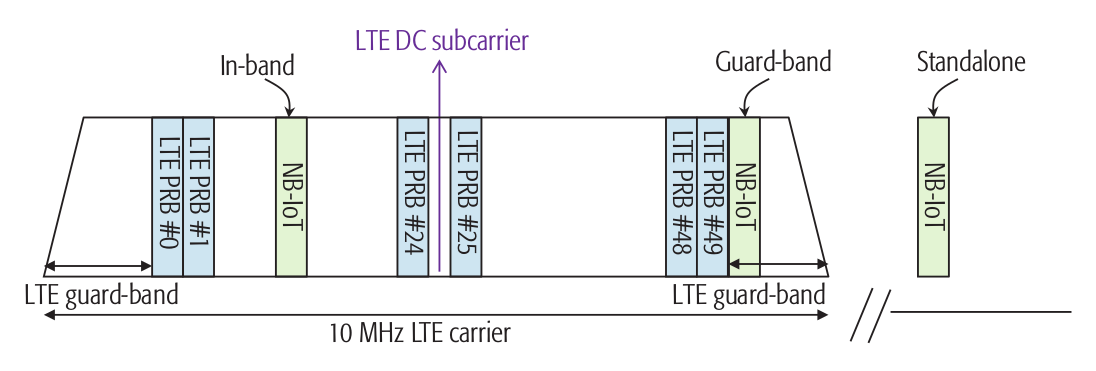
\includegraphics[width=\textwidth]{figures/deployment.png}
\caption{Deployment of the NB-IoT as in-band, guard-band or standalone \citep{primer}.}
\label{fig:NB deployment}
\end{figure}

To allow in-band operation, the physical layer of \gls{NB-IoT} needs to follow the overall structure of \gls{LTE}. To describe this, it is split into the \gls{DL} and \gls{UL} part. First the \gls{DL} part will be investigated as this accounts for most of the critical factors of the communication i.e. synchronization and system information. 

\subsubsection{Downlink}
As the primary users of legacy \gls{LTE} does not know of the \gls{NB-IoT} system, the primary concern is the interference it causes. Some structural guidelines is therefore needed when designing the \gls{NB-IoT} system, here under it needs to blend in with the \gls{OFDM} symbols of the \gls{LTE} system, meaning that timing alignment and subcarrier spacing is already determined \citep[ch. 7.2]{NB-IoT_Book}. 

Channel Raster\\
As \gls{NB-IoT} functions as an individual system, it needs it own overhead. To ensure the functionality of both systems, the \gls{PRB}s used for \gls{NB-IoT} is therefore placed outside the six center \gls{PRB}'s, as these are used for LTE synchronization. This implies that only the LTE cells with a bandwidth larger than 1.4 MHz can host NB-IoT \citep{whitepaper}. Furthermore to keep the receiver complexity and the battery consumption at a minimum, the device searches for the \gls{NB-IoT} cell on a raster of 100 kHz \citep[ch. 7.2]{NB-IoT_Book}. The center of the bandwidth host a DC-subcarrier and the \gls{PRB}'s is placed around this. This means that the center of a PRB will be offset from the raster, for instance PRB \#25 in \autoref{fig:NB deployment} has a center of 97.5 kHz, which is 2.5 kHz off from the raster. Because of this, an additional requirement is made that only those \gls{PRB}'s, where the offset is less than 7.5 kHz can be used to host a NB-IoT cell \citep{primer}. The PRB's that fulfill this criteria can be seen in \autoref{tab:available-PRBs}. 

\begin{table}[H]
\centering
\begin{tabular}{|c|p{1.8cm}|p{1.8cm}|p{1.8cm}|p{1.8cm}|p{1.8cm}|}\hline
\textbf{LTE cell bandwidth}	& 3 MHz				& 5 MHz	& 10 MHz	& 15 MHz	& 20 MHz \\\hline
Available PRB indexes		& 2, 12	& 2, 7, 17, 22	& 4, 9, 14, 19, 30, 35, 40, 45 & 2, 7, 12, 17, 22, 27, 32, 42, 47, 52, 57, 62, 67, 72 & 4, 9, 14, 19, 24, 29, 34, 39, 44, 55, 60, 65, 70, 75, 80, 85, 90, 95 \\\hline
\end{tabular}
\caption{Available PRBs depending on the bandwidth of the LTE cell \citep{whitepaper}.}
\label{tab:available-PRBs}
\end{table}


Frame Structure\\
To fit into a \gls{LTE} \gls{PRB}, the frame structure needs to be very similar to legacy \gls{LTE}. The structure is divided into: hyperframe, frame, subframe and slots. Where two slots make a subframe, ten subframes make a frame and 1024 frames make a hyperframe. A complete cycle takes 1024 hyperframes, which corresponds to 2 hours 54 minutes and 46 seconds. This structure is shown on \autoref{fig:downlink-structure}. \citep[ch. 7.2]{NB-IoT_Book}


\begin{figure}[H]
\centering
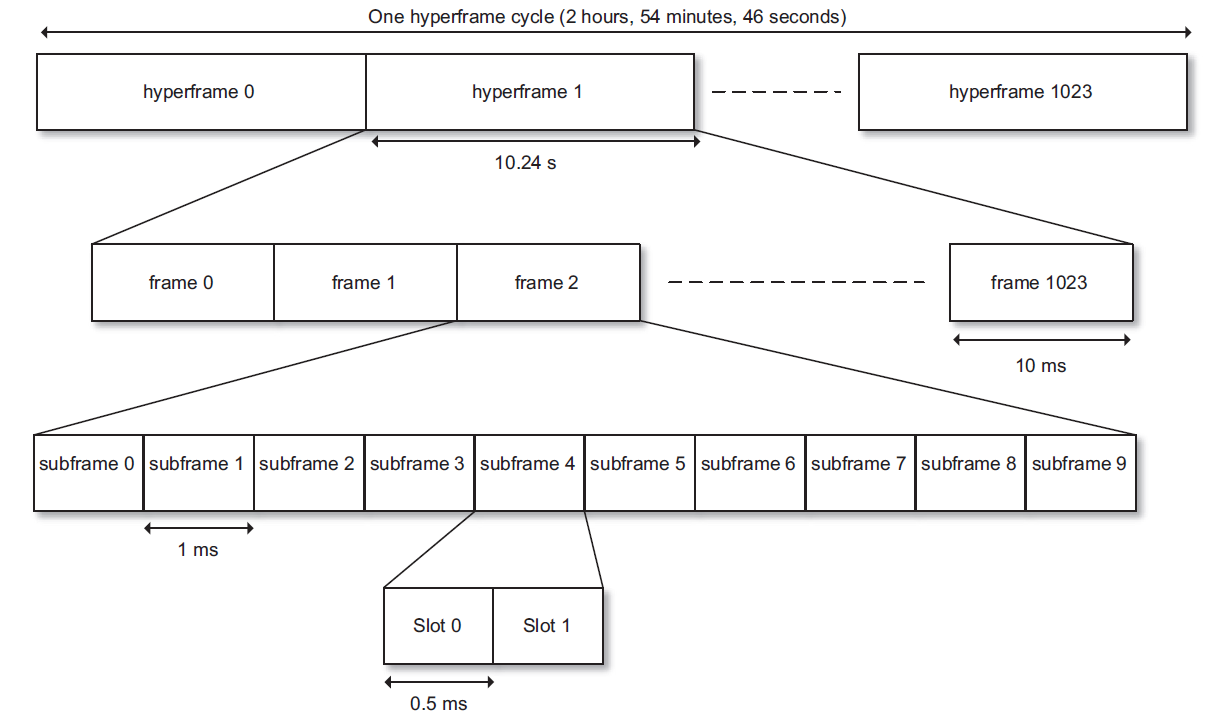
\includegraphics[width=\textwidth]{figures/downlink_structure_15kHz.png}
\caption{\gls{NB-IoT} downlink structure \citep[Fig. 7.7]{NB-IoT_Book}.}
\label{fig:downlink-structure}
\end{figure}


As the \gls{NB-IoT} system is placed outside the \gls{PRB}s used for LTE synchronization, most of the subframes are available to use, with the only exception being when a \gls{MBSFN} is present, which can occupy either of subframes (1,2,3,6,7,8) \citep{LTE-MBSFN}. Therefore the \gls{NPSS} and \gls{NSSS} is placed in subframe 5 and 9 respectively as seen on \autoref{fig:frame-structure}. By having the \gls{NSSS} being present only in even numbered frame, the \gls{LSB} of the frame numbers can be deduced directly. This increases the efficiency of the system by freeing subframe 9 in odd numbered frames and omitting that bit from the \gls{NB-IoT} overhead. The \gls{NPBCH} is located in the subframe 0 and contains the \gls{MIB-NB} \citep{REL-13}.  

\tikzsetnextfilename{frameStructure}
\begin{figure}[H]
\centering
\definecolor{NPSS}{HTML}{00D0FF}
\definecolor{NSSS}{HTML}{F97BFF}
\definecolor{NPBCH}{HTML}{92D050}
\usetikzlibrary{patterns,decorations.pathreplacing}

\resizebox{\textwidth}{!}{
\begin{tikzpicture}[scale = 0.4]

\draw [thick,decoration={brace,mirror,raise=0.1cm},decorate] (-20,-4) -- (-16,-4) node [pos=0.5,anchor=north,yshift=-0.1cm] {1 ms}; 
\draw [thick,decoration={brace,mirror,raise=0.2cm},decorate] (-20,-5) -- (20,-5) node [pos=0.5,anchor=north,yshift=-0.3cm] {10 ms};



\draw[fill = NPBCH]  (-20,2) rectangle (-16,0);
\draw  (-16,2) rectangle (-12,0);
\draw  (-12,2) rectangle (-8,0);
\draw  (-8,2) rectangle (-4,0);
\draw  (-4,2) rectangle (0,0);
\draw[fill = NPSS]  (0,2) rectangle (4,0);
\draw  (4,2) rectangle (8,0);
\draw  (8,2) rectangle (12,0);
\draw  (12,2) rectangle (16,0);
\draw[fill = NSSS]  (16,2) rectangle (20,0);

\draw[fill = NPBCH]  (-20,-2) rectangle (-16,-4);
\draw  (-16,-2) rectangle (-12,-4);
\draw  (-12,-2) rectangle (-8,-4);
\draw  (-8,-2) rectangle (-4,-4);
\draw  (-4,-2) rectangle (0,-4);
\draw[fill = NPSS]  (0,-2) rectangle (4,-4);
\draw  (4,-2) rectangle (8,-4);
\draw  (8,-2) rectangle (12,-4);
\draw  (12,-2) rectangle (16,-4);
\draw  (16,-2) rectangle (20,-4);

\node at (-18,3) {0};
\node at (-14,3) {1};
\node at (-10,3) {2};
\node at (-6,3) {3};
\node at (-2,3) {4};
\node at (2,3) {5};
\node at (6,3) {6};
\node at (10,3) {7};
\node at (14,3) {8};
\node at (18,3) {9};
\node at (-22,1) {even};
\node at (-22,-3) {odd};
\node [rotate = 90] at (-24,-1) {\textbf{Frame number}}; 

\node at (-18,1) {\acrshort{NPBCH}};
\node at (-18,-3) {\acrshort{NPBCH}};
\node at (2,1) {\acrshort{NPSS}};
\node at (2,-3) {\acrshort{NPSS}};
\node at (18,1) {\acrshort{NSSS}};
\node at (-14,1) {*};
\node at (-10,1) {*};
\node at (-6,1) {*};
\node at (-2,1) {*};
\node at (6,1) {*};
\node at (10,1) {*};
\node at (14,1) {*};
\node at (-14,-3) {*};
\node at (-10,-3) {*};
\node at (-6,-3) {*};
\node at (-2,-3) {*};
\node at (6,-3) {*};
\node at (10,-3) {*};
\node at (14,-3) {*};
\node at (18,-3) {*};
\node at (0,4.5) {\textbf{Subframe number}}; 

\node at (-15,-7) {* \acrshort{NPDCCH}/\acrshort{NPDSCH}};
\end{tikzpicture}
}

\caption{\gls{NB-IoT} frame structure \citep{REL-13}.}
\label{fig:frame-structure}
\end{figure}


By zooming in on a subframe, it is possible to see how the different \gls{OFDM} symbols is utilized. During a subframe, 14 \gls{OFDM} symbols are transmitted, each having 12 subcarriers, which results in 168 \gls{RE} per subframe. As can be seen on \autoref{fig:subframe-structure}, almost half of the \gls{RE} in a subframe might be reserved for different signals and \gls{LTE} control information \citep{REL-13}. An \gls{LTE} cell can allocate up to three symbols for \gls{PDCCH} and might use up to four carrier, which needs four \gls{RS}s \citep{whitepaper}. The \gls{NB-IoT} structure allows for up to two carriers and needs therefore two \gls{RS} namely \gls{NRS}1 and \gls{NRS}2 \citep{REL-13}. The placement of all these signals can be seen in \autoref{fig:subframe-structure}.  

\tikzsetnextfilename{subframe}
\begin{figure}[H]
\centering
\definecolor{LTERS}{HTML}{496d22}
\definecolor{LTECCH}{HTML}{92D050}
\definecolor{NPSS}{HTML}{00D0FF}
\definecolor{NSSS}{HTML}{F97BFF}


\resizebox{\textwidth}{!}{
\begin{tikzpicture}[scale=0.5]

\draw[pattern=north west lines, pattern color=LTECCH]  (-21,9) rectangle (-12,-9);
\draw [thick,decoration={brace,mirror},decorate] (-25.5,9) -- (-25.5,-9) node [pos=0.5,anchor=east, xshift=-0.1cm] {180 kHz};
\draw [thick,decoration={brace,mirror,raise=0.1cm},decorate] (-22.2,-7.5) -- (-22.2,-9) node [pos=0.5,anchor=east,xshift=-0.1cm] {15 kHz};
\draw [thick,decoration={brace,mirror,raise=0.1cm},decorate] (-21,-9.5) -- (-18,-9.5) node [pos=0.5,anchor=north,yshift=-0.2cm] {66.7 $\mu$ s};
\draw [thick,decoration={brace,mirror,raise=0.1cm},decorate] (-21,-11) -- (21,-11) node [pos=0.5,anchor=north,yshift=-0.2cm] {1 ms};


\node[text =red] at (-10.5,11) {Slot 0};
\node[text =red] at (10,11) {Slot 1};

%række 11
\draw  (-21,9) rectangle (-18,7.5);
\draw  (-18,9) rectangle (-15,7.5);
\draw  (-15,9) rectangle (-12,7.5);
\draw  (-12,9) rectangle (-9,7.5);
\draw  (-9,9) rectangle (-6,7.5);
\draw  (-6,9) rectangle (-3,7.5);
\draw  (-3,9) rectangle (0,7.5);
\draw  (-0,9) node (v1) {} rectangle (3,7.5);
\draw  (3,9) rectangle (6,7.5);
\draw  (6,9) rectangle (9,7.5);
\draw  (9,9) rectangle (12,7.5);
\draw  (12,9) rectangle (15,7.5);
\draw  (15,9) rectangle (18,7.5);
\draw  (18,9) rectangle (21,7.5);

%række 10
\draw  (-21,7.5) rectangle (-18,6);
\draw  (-18,7.5) rectangle (-15,6);
\draw  (-15,7.5) rectangle (-12,6);
\draw  (-12,7.5) rectangle (-9,6);
\draw  (-9,7.5) rectangle (-6,6);
\draw  (-6,7.5) rectangle (-3,6);
\draw  (-3,7.5) rectangle (0,6);
\draw  (-0,7.5) rectangle (3,6);
\draw  (3,7.5) rectangle (6,6);
\draw  (6,7.5) rectangle (9,6);
\draw  (9,7.5) rectangle (12,6);
\draw  (12,7.5) rectangle (15,6);
\draw  (15,7.5) rectangle (18,6);
\draw  (18,7.5) rectangle (21,6);

%række 9
\draw[pattern=north west lines, pattern color=LTERS] (-21,6) rectangle (-18,4.5);
\draw[pattern=north west lines, pattern color=LTERS] (-18,6) rectangle (-15,4.5);
\draw  (-15,6) rectangle (-12,4.5);
\draw  (-12,6) rectangle (-9,4.5);
\draw[pattern=north west lines, pattern color=LTERS]  (-9,6) rectangle (-6,4.5);
\draw[pattern=north west lines, pattern color=NSSS]  (-6,6) rectangle (-3,4.5);
\draw[pattern=north west lines, pattern color=NPSS]  (-3,6) rectangle (0,4.5);
\draw[pattern=north west lines, pattern color=LTERS]  (-0,6) rectangle (3,4.5);
\draw[pattern=north west lines, pattern color=LTERS]  (3,6) rectangle (6,4.5);
\draw  (6,6) rectangle (9,4.5);
\draw  (9,6) rectangle (12,4.5);
\draw[pattern=north west lines, pattern color=LTERS]  (12,6) rectangle (15,4.5);
\draw[pattern=north west lines, pattern color=NSSS] (15,6) rectangle (18,4.5);
\draw[pattern=north west lines, pattern color=NPSS]  (18,6) rectangle (21,4.5);

%række 8
\draw  (-21,4.5) rectangle (-18,3);
\draw  (-18,4.5) rectangle (-15,3);
\draw  (-15,4.5) rectangle (-12,3);
\draw  (-12,4.5) rectangle (-9,3);
\draw  (-9,4.5) rectangle (-6,3);
\draw  (-6,4.5) rectangle (-3,3);
\draw  (-3,4.5) rectangle (0,3);
\draw  (-0,4.5) rectangle (3,3);
\draw  (3,4.5) rectangle (6,3);
\draw  (6,4.5) rectangle (9,3);
\draw  (9,4.5) rectangle (12,3);
\draw  (12,4.5) rectangle (15,3);
\draw  (15,4.5) rectangle (18,3);
\draw  (18,4.5) rectangle (21,3);

%række 7
\draw  (-21,3) rectangle (-18,1.5);
\draw  (-18,3) rectangle (-15,1.5);
\draw  (-15,3) rectangle (-12,1.5);
\draw  (-12,3) rectangle (-9,1.5);
\draw  (-9,3) rectangle (-6,1.5);
\draw  (-6,3) rectangle (-3,1.5);
\draw  (-3,3) rectangle (0,1.5);
\draw  (-0,3) rectangle (3,1.5);
\draw  (3,3) rectangle (6,1.5);
\draw  (6,3) rectangle (9,1.5);
\draw  (9,3) rectangle (12,1.5);
\draw  (12,3) rectangle (15,1.5);
\draw  (15,3) rectangle (18,1.5);
\draw  (18,3) rectangle (21,1.5);

%række 6
\draw[pattern=north west lines, pattern color=LTERS] (-21,1.5) rectangle (-18,0);
\draw[pattern=north west lines, pattern color=LTERS] (-18,1.5) rectangle (-15,0);
\draw  (-15,1.5) rectangle (-12,0);
\draw  (-12,1.5) rectangle (-9,0);
\draw[pattern=north west lines, pattern color=LTERS]  (-9,1.5) rectangle (-6,0);
\draw[pattern=north west lines, pattern color=NPSS]  (-6,1.5) rectangle (-3,0);
\draw[pattern=north west lines, pattern color=NSSS]  (-3,1.5) rectangle (0,0);
\draw[pattern=north west lines, pattern color=LTERS]  (-0,1.5) rectangle (3,0);
\draw[pattern=north west lines, pattern color=LTERS]  (3,1.5) rectangle (6,0);
\draw  (6,1.5) rectangle (9,0);
\draw  (9,1.5) rectangle (12,0);
\draw[pattern=north west lines, pattern color=LTERS]  (12,1.5) rectangle (15,0);
\draw[pattern=north west lines, pattern color=NPSS]  (15,1.5) rectangle (18,0);
\draw[pattern=north west lines, pattern color=NSSS] (18,1.5) rectangle (21,0);

%række 5
\draw  (-21,-0) rectangle (-18,-1.5);
\draw  (-18,-0) rectangle (-15,-1.5);
\draw  (-15,-0) rectangle (-12,-1.5);
\draw  (-12,-0) rectangle (-9,-1.5);
\draw  (-9,-0) rectangle (-6,-1.5);
\draw  (-6,-0) rectangle (-3,-1.5);
\draw  (-3,-0) rectangle (0,-1.5);
\draw  (-0,-0) rectangle (3,-1.5);
\draw  (3,-0) rectangle (6,-1.5);
\draw  (6,-0) rectangle (9,-1.5);
\draw  (9,-0) rectangle (12,-1.5);
\draw  (12,-0) rectangle (15,-1.5);
\draw  (15,-0) rectangle (18,-1.5);
\draw  (18,-0) rectangle (21,-1.5);

%række 4
\draw  (-21,-1.5) rectangle (-18,-3);
\draw  (-18,-1.5) rectangle (-15,-3);
\draw  (-15,-1.5) rectangle (-12,-3);
\draw  (-12,-1.5) rectangle (-9,-3);
\draw  (-9,-1.5) rectangle (-6,-3);
\draw  (-6,-1.5) rectangle (-3,-3);
\draw  (-3,-1.5) rectangle (0,-3);
\draw  (-0,-1.5) rectangle (3,-3);
\draw  (3,-1.5) rectangle (6,-3);
\draw  (6,-1.5) rectangle (9,-3);
\draw  (9,-1.5) rectangle (12,-3);
\draw  (12,-1.5) rectangle (15,-3);
\draw  (15,-1.5) rectangle (18,-3);
\draw  (18,-1.5) rectangle (21,-3);

%række 3
\draw[pattern=north west lines, pattern color=LTERS] (-21,-3) rectangle (-18,-4.5);
\draw[pattern=north west lines, pattern color=LTERS] (-18,-3) rectangle (-15,-4.5);
\draw  (-15,-3) rectangle (-12,-4.5);
\draw  (-12,-3) rectangle (-9,-4.5);
\draw[pattern=north west lines, pattern color=LTERS]  (-9,-3) rectangle (-6,-4.5);
\draw[pattern=north west lines, pattern color=NSSS]  (-6,-3) rectangle (-3,-4.5);
\draw[pattern=north west lines, pattern color=NPSS]  (-3,-3) rectangle (0,-4.5);
\draw[pattern=north west lines, pattern color=LTERS]  (-0,-3) rectangle (3,-4.5);
\draw[pattern=north west lines, pattern color=LTERS]  (3,-3) rectangle (6,-4.5);
\draw  (6,-3) rectangle (9,-4.5);
\draw  (9,-3) rectangle (12,-4.5);
\draw[pattern=north west lines, pattern color=LTERS]  (12,-3) rectangle (15,-4.5);
\draw[pattern=north west lines, pattern color=NSSS]  (15,-3) rectangle (18,-4.5);
\draw[pattern=north west lines, pattern color=NPSS]  (18,-3) rectangle (21,-4.5);

%række 2
\draw  (-21,-4.5) rectangle (-18,-6);
\draw  (-18,-4.5) rectangle (-15,-6);
\draw  (-15,-4.5) rectangle (-12,-6);
\draw  (-12,-4.5) rectangle (-9,-6);
\draw  (-9,-4.5) rectangle (-6,-6);
\draw  (-6,-4.5) rectangle (-3,-6);
\draw  (-3,-4.5) rectangle (0,-6);
\draw  (-0,-4.5) rectangle (3,-6);
\draw  (3,-4.5) rectangle (6,-6);
\draw  (6,-4.5) rectangle (9,-6);
\draw  (9,-4.5) rectangle (12,-6);
\draw  (12,-4.5) rectangle (15,-6);
\draw  (15,-4.5) rectangle (18,-6);
\draw  (18,-4.5) rectangle (21,-6);

%række 1
\draw  (-21,-6) rectangle (-18,-7.5);
\draw  (-18,-6) rectangle (-15,-7.5);
\draw  (-15,-6) rectangle (-12,-7.5);
\draw  (-12,-6) rectangle (-9,-7.5);
\draw  (-9,-6) rectangle (-6,-7.5);
\draw  (-6,-6) rectangle (-3,-7.5);
\draw  (-3,-6) rectangle (0,-7.5);
\draw  (-0,-6) rectangle (3,-7.5);
\draw  (3,-6) rectangle (6,-7.5);
\draw  (6,-6) rectangle (9,-7.5);
\draw  (9,-6) rectangle (12,-7.5);
\draw  (12,-6) rectangle (15,-7.5);
\draw  (15,-6) rectangle (18,-7.5);
\draw  (18,-6) rectangle (21,-7.5);

%række 0
\draw[pattern=north west lines, pattern color=LTERS] (-21,-7.5) rectangle (-18,-9);
\draw[pattern=north west lines, pattern color=LTERS] (-18,-7.5) rectangle (-15,-9);
\draw  (-15,-7.5) rectangle (-12,-9); 
\draw  (-12,-7.5) rectangle (-9,-9);
\draw[pattern=north west lines, pattern color=LTERS]  (-9,-7.5) rectangle (-6,-9);
\draw[pattern=north west lines, pattern color=NPSS]  (-6,-7.5) rectangle (-3,-9);
\draw[pattern=north west lines, pattern color=NSSS]  (-3,-7.5) rectangle (0,-9) node (v2) {};
\draw[pattern=north west lines, pattern color=LTERS]  (-0,-7.5) rectangle (3,-9);
\draw[pattern=north west lines, pattern color=LTERS]  (3,-7.5) rectangle (6,-9);
\draw  (6,-7.5) rectangle (9,-9);
\draw  (9,-7.5) rectangle (12,-9);
\draw[pattern=north west lines, pattern color=LTERS]  (12,-7.5) rectangle (15,-9);
\draw[pattern=north west lines, pattern color=NPSS]  (15,-7.5) rectangle (18,-9);
\draw[pattern=north west lines, pattern color=NSSS]  (18,-7.5) rectangle (21,-9);


\node at (-22,-8.25) {0};
\node at (-22,-6.75) {1};
\node at (-22,-5.25) {2};
\node at (-22,-3.75) {3};
\node at (-22,-2.25) {4};
\node at (-22,-0.75) {5};
\node at (-22,0.75) {6};
\node at (-22,2.25) {7};
\node at (-22,3.75) {8};
\node at (-22,5.25) {9};
\node at (-22,6.75) {10};
\node at (-22,8.25) {11};

\node at (-19.5,10) {0};
\node at (-16.5,10) {1};
\node at (-13.5,10) {2};
\node at (-10.5,10) {3};
\node at (-7.5,10) {4};
\node at (-4.5,10) {5};
\node at (-1.5,10) {6};
\node at (1.5,10) {7};
\node at (4.5,10) {8};
\node at (7.5,10) {9};
\node at (10.5,10) {10};
\node at (13.5,10) {11};
\node at (16.5,10) {12};
\node at (19.5,10) {13};

\draw[draw=red,line width=2pt] (0,9) -- (0,-9);
\draw[pattern=north west lines, pattern color=LTERS]  (-21,-13) rectangle (-18,-14.5);
\draw[pattern=north west lines, pattern color=LTECCH]  (-13,-13) rectangle (-10,-14.5);
\draw[pattern=north west lines, pattern color=NPSS]  (-3.5,-13) rectangle (-0.5,-14.5) ;
\draw[pattern=north west lines, pattern color=NSSS]  (4,-13) rectangle (7,-14.5) ;
\draw (11.5,-13) rectangle (14.5,-14.5);

\node[anchor=west] at (-17.5,-13.75) {\acrshort{LTE} \acrshort{RS}};
\node[anchor=west] at (-9.5,-13.75) {\acrshort{LTE} \acrshort{PDCCH}};
\node[anchor=west] at (-0,-13.75) {\acrshort{NRS}1};
\node[anchor=west] at (7.5,-13.75) {\acrshort{NRS}2};
\node[anchor=west] at (15,-13.75) {Free symbol};

\end{tikzpicture}
}
\caption{The structure of a \gls{DL} subframe \citep{whitepaper,REL-13}.}
\label{fig:subframe-structure}
\end{figure}

It should be noted that the described allocation is a worst case scenario for the \gls{DL}. If the system is deployed either in guard-band or as stand-alone, only the \gls{NRS} is actually used, but before the device is synchronized, it does not know what is in use and needs to guard for this worst case scenario. When the device receives the \gls{MIB-NB} and \gls{NB-SIB}1 it will get information in regards to the number of carriers and the size of \gls{LTE} \gls{PDCCH} \citep{whitepaper}. 

Channels\\ 
As shown on \autoref{fig:frame-structure}, three channels exist in the physical \gls{DL} part of the protocol. These are respectively: \gls{NPBCH}, \gls{NPDCCH} and \gls{NPDSCH}. The structure of the \gls{NPBCH} is explained in the \autoref{sec:Network_access}.

The \gls{NPDCCH} carries three types of information: one is use to indicate \gls{DL} scheduling for the devices, one provides \gls{UL} grant information and the last indicates paging or system information update \citep{NB-IoT_Book}. It should be noted that  depending on the coverage level the \gls{NPDCCH} might be repeated up 2048 times \citep{NB-IoT_Book}.

The \gls{NPDSCH} is used to transmit data when an bearer is established. Depending on the coverage level the \gls{NPDSCH} might be repeated up 2048 times. A \gls{TBS} may be up to 680 bits depending on the \gls{TBS} index and the number of subframes used. \citep{NB-IoT_Book}

\subsubsection{Uplink}
\label{sec:ULphy}
As mentioned in \autoref{ch:Introduction}, most of the data in the system is \gls{UL} data. Therefore is the \gls{UL} spectrum tuned to accommodate the massive number of devices. The timing alignment of the \gls{UL} follows the \gls{DL} meaning when synchronized to the \gls{DL} band, the device is also synchronized to the \gls{UL}, except for the delay introduced by the travelling time of the signal. This delay is found at the beginning of the \gls{RAP}, which will be further explained in \autoref{sec:RAP}. 

Frame Structure\\
Compared to legacy \gls{LTE}, two differences should be noted. The channel \gls{PUCCH} has been removed and the \gls{UL} frame can take different formats. It is 180 kHz wide, as the \gls{DL} frame, however the sub carrier spacing can be both 3.75 kHz and 15 kHz, giving 48 and 12 subcarriers respectively. This is however only done on the \gls{NPUSCH}, in the \gls{NPRACH} the subcarrier spacing is always 3.75 kHz \citep{NB-IoT_Book}. For each symbol that is transmitted, a \gls{CP} is used. The structure of the channels can be seen on \autoref{fig:NPUSCH1_structure}, \autoref{fig:NPUSCH2_structure} and \autoref{fig:NPRACH_structure}.

\begin{minipage}{0.48\textwidth}
\begin{figure}[H]
\centering
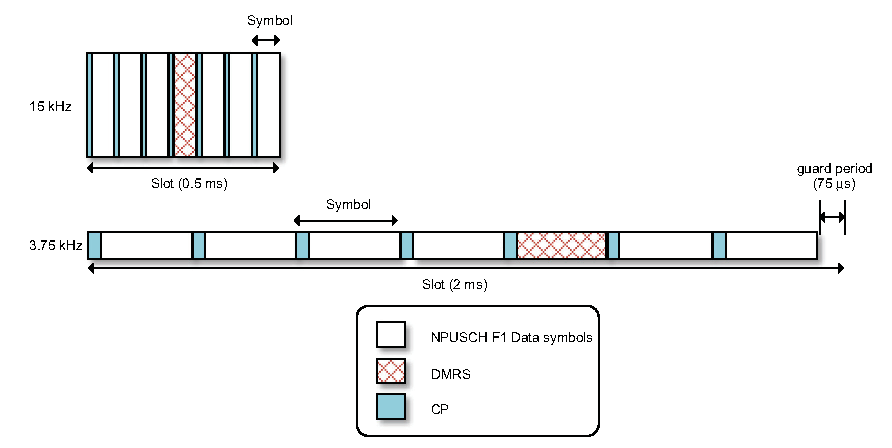
\includegraphics[width=\textwidth]{figures/NPUSCH1_structure.pdf}
\caption{The structure of NPUSCH format 1 \citep{NB-IoT_Book}}
\label{fig:NPUSCH1_structure}
\end{figure}
\end{minipage}%
\hfill
\begin{minipage}{0.48\textwidth}
\begin{figure}[H]
\centering
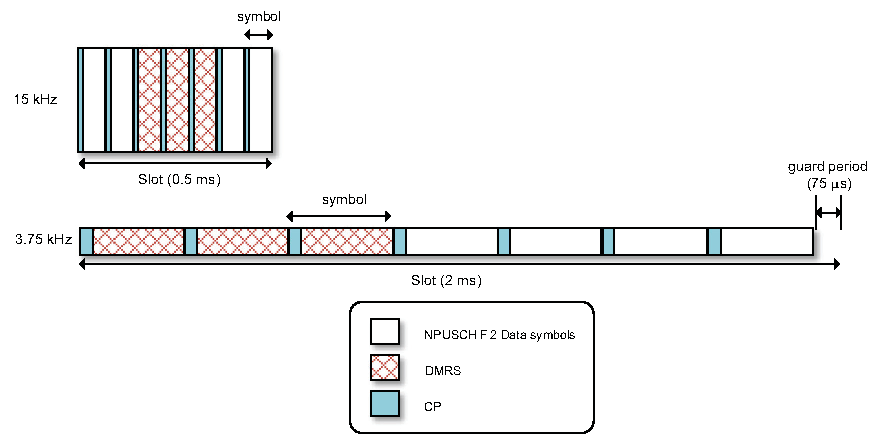
\includegraphics[width=\textwidth]{figures/NPUSCH2_structure.pdf}
\caption{The structure of NPUSCH format 2 \citep{NB-IoT_Book}}
\label{fig:NPUSCH2_structure}
\end{figure}
\end{minipage}


\begin{figure}[H]
\centering
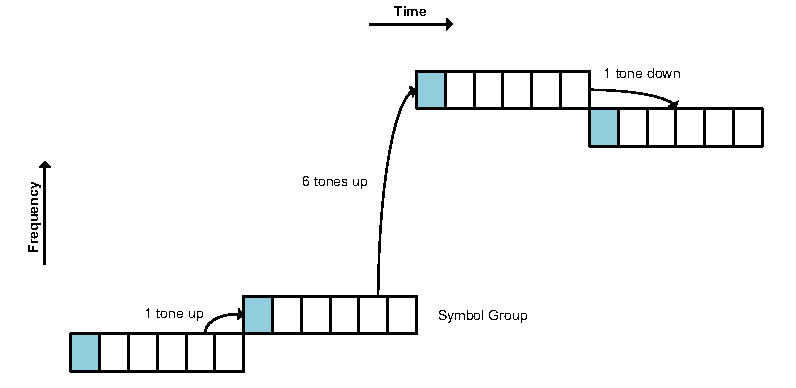
\includegraphics[width=0.5\textwidth]{figures/NPRACH_frequency_hopping.pdf}
\caption{The structure of a NPRACH symbol group \citep{NB-IoT_Book}}
\label{fig:NPRACH_structure}
\end{figure}

Channels\\
The \gls{UL} consists of two channels and one signal, namely the \gls{NPRACH}, \gls{NPUSCH} and \gls{DMRS}.

The \gls{NPRACH} consist of a repetition of four symbol groups, for each symbol group a \gls{CP} is attached followed by five symbols. The duration of the CP is dependent on the CP-format chosen this can be seen in \autoref{fig:NPRACH_structure}, and depending on the coverage level the \gls{NPRACH} might be repeated up to 128 times. The NPRACH only uses 12 subcarriers at any time, which are used for msg1 in the \gls{NRAP}, see \autoref{sec:RAP}. \citep{NB-IoT_Book}

The \gls{NPUSCH} carries the data transmitted form the device and \gls{HARQ} acknowledgement from the \gls{NPDSCH}, this is referred to as format 1 and 2 respectively. Format 1 can carry up 1000 bits per \gls{TB}. As seen on \autoref{fig:NPUSCH1_structure} and \autoref{fig:NPUSCH2_structure} the DMRS, which is used for channel estimation at the base station, is multiplexed with the NPUSCH. 






\section{Network Access}
\label{sec:Network_access}
This section describes the different procedures needed to navigate in the NB-IoT framework. This is the procedure to establish a connection as well as the procedures to navigate between different connection states. 

\subsection{Cell Search and Synchronization Procedure}
\label{sec:cellsync}
The first thing needed of a device is to locate a cell, this is done during the as part of the synchronization procedure. The synchronization procedure is very similar to that of a \gls{LTE} as can be seen in \autoref{fig:sync-NB}, as the device first needs to search for the cell and then acquire the system information. 


\tikzsetnextfilename{sync-NB}
\begin{figure}[H]
\centering
\definecolor{top}{HTML}{00FFFF}
\definecolor{center}{HTML}{0080FF}
\definecolor{bund}{HTML}{0000FF}
\usetikzlibrary{arrows}

%\resizebox{0.5\textwidth}{!}{
\begin{tikzpicture}[scale = 0.4]

\draw (-7.5,8) rectangle (-2.5,6);
\node at (-5,7) {Device};
\draw [dashed] (-5,6) -- (-5,-4);

\draw (2.5,8) rectangle (7.5,6);
\node at (5,7) {\acrshort{eNB}};
\draw [dashed] (5,6) -- (5,-4);

\draw[arrows={triangle 45-}] (-5,4) -- (5,4);
\node at (0,4.5) {\acrshort{NPSS}};

\draw[arrows={triangle 45-}] (-5,2) -- (5,2);
\node at (0,2.5) {\acrshort{NSSS}};

\draw[arrows={triangle 45-}] (-5,0) -- (5,0);
\node at (0,0.5) {\acrshort{MIB-NB}};

\draw[arrows={triangle 45-}] (-5,-2) -- (5,-2);
\node at (0,-1.5) {\acrshort{NB-SIB}s};

\end{tikzpicture}
%}

\caption{The process needed to synchronize to a cell.}
\label{fig:sync-NB}
\end{figure}

The device first looks for the \gls{NPSS}, the search spaces for the \gls{NPSS} is predetermined based on the LTE bands. \todo{make ref to LTE bands} This provides the initial \gls{CFO} as well as a 10 ms timing alignment. As mentioned the NPSS takes up the entire fifth subframe of each frame, a frequency domain Zadoff-Chu sequence is used for the 11 available \gls{OFDM} symbols, as the first 3 OFDM might be used for LTE PDCCH. For low complexity devices a single 10 ms segment might not suffice at a low \gls{SNR}, the structure of the \gls{NPSS} is therefore made so the signals can accumulate coherently over multiple 10 ms segments. \citep{NB-IoT_Book,primer}. The \gls{NSSS} is also based on a frequency domain Zadoff-Chu sequence, but is further scrambled based on the \gls{NB-PCID}. This means the device has to manually try each frequency and then manually test for each of the 504 NB-PCID. When this is done the device will be frequency and in a 80 ms window time synchronized with the eNB and know the NB-PCID also \citep{NB-IoT_Book,primer}. 

The next step is to decode the \gls{MIB-NB}, it consists of 34 bits and 16 \gls{CRC} bits, they are transmitted in eight self-decodeable blocks which is repeated eight times resulting in a total transmission time of 640 ms as can be seen on \autoref{fig:MIB-NB}. 
 
\tikzsetnextfilename{MIB-NB}
\begin{figure}[H]
\centering
\definecolor{top}{HTML}{00FFFF}
\definecolor{center}{HTML}{0080FF}
\definecolor{bund}{HTML}{0000FF}
\usetikzlibrary{arrows}

\resizebox{\textwidth}{!}{
\begin{tikzpicture}[scale = 0.4]

\draw [fill=top] (-20,8) rectangle (20,6);
\node at (0,7) {\acrshort{MIB-NB}};
\draw (-20,10) -- (-20,8);
\draw (20,10) -- (20,8);
\node (top) at (0,9) {640 ms};
\draw[arrows={-triangle 45}] (top) edge (-20,9);
\draw[arrows={-triangle 45}] (top) edge (20,9);

\draw (0,6) -- (0,4); 
\draw (-17.5,4) -- (17.5,4);

\draw[arrows={-triangle 45}] (-17.5,4) -- (-17.5,2);
\draw[arrows={-triangle 45}] (-12.5,4) -- (-12.5,2);
\draw[arrows={-triangle 45}] (-7.5,4) -- (-7.5,2);
\draw[arrows={-triangle 45}] (-2.5,4) -- (-2.5,2);
\draw[arrows={-triangle 45}] (2.5,4) -- (2.5,2);
\draw[arrows={-triangle 45}] (7.5,4) -- (7.5,2);
\draw[arrows={-triangle 45}] (12.5,4) -- (12.5,2);
\draw[arrows={-triangle 45}] (17.5,4) -- (17.5,2);

\draw [fill=center] (-20,2) rectangle (-15,0);
\draw [fill=center] (-15,2) rectangle (-10,0);
\draw [fill=center] (-10,2) rectangle (-5,0);
\draw [fill=center] (-5,2) rectangle (0,0);
\draw [fill=center] (0,2) rectangle (5,0);
\draw [fill=center] (5,2) rectangle (10,0);
\draw [fill=center] (10,2) rectangle (15,0);
\draw [fill=center] (15,2) rectangle (20,0);

\node at (-17.5,1) {BL1};
\node at (-12.5,1) {BL2};
\node at (-7.5,1) {BL3};
\node at (-2.5,1) {BL4};
\node at (2.5,1) {BL5};
\node at (7.5,1) {BL6};
\node at (12.5,1) {BL7};
\node at (17.5,1) {BL8};

\node(bl1) at (-17.5,-1) {80 ms};
\draw[arrows={-triangle 45}] (bl1) edge (-20,-1);
\draw[arrows={-triangle 45}] (bl1) edge (-15,-1);
\draw (-15,0) -- (-15,-2);
\draw (-20,0) -- (-20,-4);
\draw (-15,-2) -- (20,-4);

\draw [fill=bund] (-20,-4) rectangle (-19.5,-6);
\draw [fill=bund] (-15,-4) rectangle (-14.5,-6);
\draw [fill=bund] (-10,-4) rectangle (-9.5,-6);
\draw [fill=bund] (-5,-4) rectangle (-4.5,-6);
\draw [fill=bund] (0,-4) rectangle (0.5,-6);
\draw [fill=bund] (5,-4) rectangle (5.5,-6);
\draw [fill=bund] (10,-4) rectangle (10.5,-6);
\draw [fill=bund] (15,-4) rectangle (15.5,-6);

\draw (-19.5,-4) rectangle (-19,-6);
\draw (-19,-4) rectangle (-18.5,-6);
\draw (-18.5,-4) rectangle (-18,-6);
\draw (-18,-4) rectangle (-17.5,-6);
\draw (-17.5,-4) rectangle (-17,-6);
\draw (-17,-4) rectangle (-16.5,-6);
\draw (-16.5,-4) rectangle (-16,-6);
\draw (-16,-4) rectangle (-15.5,-6);
\draw (-15.5,-4) rectangle (-15,-6);

\draw (-14.5,-4) rectangle (-14,-6);
\draw (-14,-4) rectangle (-13.5,-6);
\draw (-13.5,-4) rectangle (-13,-6);
\draw (-13,-4) rectangle (-12.5,-6);
\draw (-12.5,-4) rectangle (-12,-6);
\draw (-12,-4) rectangle (-11.5,-6);
\draw (-11.5,-4) rectangle (-11,-6);
\draw (-11,-4) rectangle (-10.5,-6);
\draw (-10.5,-4) rectangle (-10,-6);

\draw (-9.5,-4) rectangle (-9,-6);
\draw (-9,-4) rectangle (-8.5,-6);
\draw (-8.5,-4) rectangle (-8,-6);
\draw (-8,-4) rectangle (-7.5,-6);
\draw (-7.5,-4) rectangle (-7,-6);
\draw (-7,-4) rectangle (-6.5,-6);
\draw (-6.5,-4) rectangle (-6,-6);
\draw (-6,-4) rectangle (-5.5,-6);
\draw (-5.5,-4) rectangle (-5,-6);

\draw (-4.5,-4) rectangle (-4,-6);
\draw (-4,-4) rectangle (-3.5,-6);
\draw (-3.5,-4) rectangle (-3,-6);
\draw (-3,-4) rectangle (-2.5,-6);
\draw (-2.5,-4) rectangle (-2,-6);
\draw (-2,-4) rectangle (-1.5,-6);
\draw (-1.5,-4) rectangle (-1,-6);
\draw (-1,-4) rectangle (-0.5,-6);
\draw (-0.5,-4) rectangle (-0,-6);

\draw (0.5,-4) rectangle (1,-6);
\draw (1,-4) rectangle (1.5,-6);
\draw (1.5,-4) rectangle (2,-6);
\draw (2,-4) rectangle (2.5,-6);
\draw (2.5,-4) rectangle (3,-6);
\draw (3,-4) rectangle (3.5,-6);
\draw (3.5,-4) rectangle (4,-6);
\draw (4,-4) rectangle (4.5,-6);
\draw (4.5,-4) rectangle (5,-6);

\draw (5.5,-4) rectangle (6,-6);
\draw (6,-4) rectangle (6.5,-6);
\draw (6.5,-4) rectangle (7,-6);
\draw (7,-4) rectangle (7.5,-6);
\draw (7.5,-4) rectangle (8,-6);
\draw (8,-4) rectangle (8.5,-6);
\draw (8.5,-4) rectangle (9,-6);
\draw (9,-4) rectangle (9.5,-6);
\draw (9.5,-4) rectangle (10,-6);

\draw (10.5,-4) rectangle (11,-6);
\draw (11,-4) rectangle (11.5,-6);
\draw (11.5,-4) rectangle (12,-6);
\draw (12,-4) rectangle (12.5,-6);
\draw (12.5,-4) rectangle (13,-6);
\draw (13,-4) rectangle (13.5,-6);
\draw (13.5,-4) rectangle (14,-6);
\draw (14,-4) rectangle (14.5,-6);
\draw (14.5,-4) rectangle (15,-6);

\draw (15.5,-4) rectangle (16,-6);
\draw (16,-4) rectangle (16.5,-6);
\draw (16.5,-4) rectangle (17,-6);
\draw (17,-4) rectangle (17.5,-6);
\draw (17.5,-4) rectangle (18,-6);
\draw (18,-4) rectangle (18.5,-6);
\draw (18.5,-4) rectangle (19,-6);
\draw (19,-4) rectangle (19.5,-6);
\draw (19.5,-4) rectangle (20,-6);

\end{tikzpicture}
}

\caption{MIB-NB}
\label{fig:MIB-NB}
\end{figure}

The information carried in the \gls{MIB-NB} are:

\begin{tabular}{ll}\\
2 bits & hyper frame number\\
4 bits & \gls{SFN}\\
4 bits & \gls{NB-SIB}1 scheduling\\
5 bits & value tag\\
1 bit & access barrer\\
7 bits & operation mode and values\\
11 bits & reserved for future use\\
\end{tabular}

From the \gls{MIB-NB} the schedule for \gls{NB-SIB}1 is found, this is always transmitted in subframe 4 however only the frames indicated by \gls{MIB-NB} carry \gls{NB-SIB}1. The final step in the synchronization is to decode all the \gls{NB-SIB}s.

When the device have read all \gls{NB-SIB}s it has fully synchronized with the \gls{eNB}. It is mandatory for the device to have a valid version of \gls{MIB-NB} as well as \gls{NB-SIB}1-5, \gls{NB-SIB}14 and 16 is only read when required. Furthermore once connected to the system the device is not expected to update its version of the \gls{NB-SIB}s unless instructed to \citep{whitepaper}. 

When the device is synchronized it can initiate the attach procedure which will now be described. 




\subsection{Narrowband Attach Procedure} \label{sec:RAP}
Before starting the narrowband attach procedure the device measures the reference signals and determine based and some \gls{RSRP} thresholds which coverage level should be applied. The coverage level determines the power level used as well as the number of repetition used \citep{NB-IoT_Book}. The narrowband attach procedure comes in three forms, a full attach where a connection is established and all the security modes and authentication happens, a connection resume where the previously established security is used and an establishment carrying data. Each form contains some smaller steps, but can generally be divided into: \gls{NRAP} and security establishment \citep{REL-13}. The security establishment follows the same pattern as LTE and will not be further explained. The \gls{NRAP} contain five messages:
\begin{tabular}{ll}
msg1 & is the NPRACH that can happen when a NPRACH occasion exists \\
msg2 & is the \gls{RAR} informing the device of timing offsets and providing a grant for msg3 \\
msg3 & is the connection request or connection resume request \\
msg4 & is contention resolution and acknowledgement of the request \\
msg5 & is the connection establishment complete message\\
\end{tabular}

This process can also be seen on \autoref{fig:RAP}


\tikzsetnextfilename{RAP}
\begin{figure}[H]
\centering
\usetikzlibrary{arrows}

\begin{tikzpicture}[scale = 0.4]

\draw (-13.5,8) rectangle (-8.5,6);
\node at (-11,7) {Device};
\draw [dashed] (-11,6) -- (-11,-4);

\draw (8.5,8) rectangle (13.5,6);
\node at (11,7) {eNB};
\draw [dashed] (11,6) -- (11,-4);

\draw[arrows={-triangle 45}] (-11,4) -- (11,4);
\node at (0,4.5) {NPRACH (msg1)};

\draw[arrows={triangle 45-}] (-11,2) -- (11,2);
\node at (0,2.5) {RAR (msg2)};

\draw[arrows={-triangle 45}] (-11,0) -- (11,0);
\node at (0,0.5) {RRC Connection Resume Request (msg3)};

\draw[arrows={triangle 45-}] (-11,-2) -- (11,-2);
\node at (0,-1.5) {RRC Connection Resume (msg4)};

\draw[arrows={-triangle 45}] (-11,-4) -- (11,-4);
\node at (0,-3.5) {RRC Connection Resume Complete (msg5)};
\end{tikzpicture}
\caption{Message visualisation of the \gls{RAP} for connection resume.}
\label{fig:RAP}
\end{figure}

The important parts to take from this is that the device gets a \gls{Ra-RNTI} based on the preamble it selects for msg1. This identifier is used to decode the rest of the messages. During the attach procedure the device is also given a \gls{P-RNTI} and a \gls{C-RNTI}, which is used for decoding radio and paging transmission later on \citep{whitepaper}. If a control plane data transmission is desired it is transmitted during the \gls{NRAP} \citep{primer}.


\subsection{Connection Control}
A connected device needs to be able to move around the different device states as seen in \autoref{fig:UE-states}. To do this different procedures is used. The primary concern here is moving in and out of idle modes, generally when connected, a device does not want to give up on its \gls{C-RNTI} as this makes the attach sequence significantly longer, that is where control plane optimization comes in. The control plane optimization enables the device to save its \gls{AS} when it goes in idle mode, this \gls{AS} is then used again when the device resumes the connection, this feature is utilized whenever possible. 

Another important aspect is the idle modes, this is where a device is expected to spend most of its time so the power consumption here needs to be minimal. The two primary idle modes are \gls{eDRX} and \gls{PSM}, however in both modes a period of time is spent in normal DRX mode. 


\subsubsection{DRX}
When the device wants to disconnect from the network it might be required to listen for mobile terminated data, this is done through the paging channel. The DRX cycle consist of a paging opportunity and a DRX opportunity, this can be seen in \autoref{fig:DRX_structure}. 

%\tikzsetnextfilename{DRX_structure}
\begin{figure}[H]
\centering
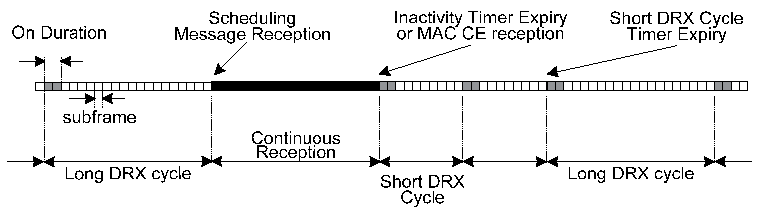
\includegraphics[width=\textwidth]{figures/DRX_structure.pdf}
\caption{The structure of \gls{DRX} idle mode \citep{book_LTE_for_UMTS2}}
\label{fig:DRX_structure}
\end{figure}

As seen on \autoref{fig:DRX_structure} several parameters define the DRX structure, the different parameters use and typical values can be found in \autoref{tab:DRX_parameters}

\begin{table}[H]
\centering
\begin{tabular}{|c|p{6cm}|p{4cm}|} \hline
\textbf{Parameter} & \textbf{Definition} & \textbf{Typical value} \\ \hline 
On duration &  the number of subframes that is monitored during the paging opportunity & 1-2 subframes\\ \hline
DRX inactivity timer & the period after a scheduling message where the device should be in continuous reception mode & 25-50 subframes \\ \hline
DRX short cycle timer & the duration of the short DRX cycle & 20-40 subframes \\ \hline
Retransmission timer & the period after a \gls{HARQ} round trip time in which the device needs to monitor the control channel & 20  subframes \\ \hline
Long DRX cycle & the duration of the short DRX cycle & 1024 subframes \\ \hline
\end{tabular}
\caption{The different parameters and their typical value when defining the DRX structure \citep{book_LTE_for_UMTS}.}
\label{tab:DRX_parameters}
\end{table}

It should be noted that these typical values are based on the DRX of LTE in NB-IoT it is uncertain if the short cycle would be used at all, and the long cycle might be as long as 10240 subframes. It is also important to note that contrary to LTE NB-IoT supports repetition of the NPDCCH channel which directly influences the paging messages. \citep{NB-IoT_Book}


\subsubsection{eDRX}
The eDRX idle mode is an extension of the DRX idle mode. It is designed to accommodate a medium length transmission interval. The build up consist of a long DRX opportunity followed by a normal DRX period often referred to as \gls{PTW}. During the long DRX opportunity only the necessary timers and PLL's to keep synchronize with the network is on, there is no need to listen to the NPDCCH for incoming data. In the \gls{PTW} the device returns to a normal DRX cycle structure and monitors the paging opportunities. This cycle can be seen on \autoref{fig:eDRX_structure}.

\tikzsetnextfilename{eDRX_structure}
\begin{figure}[H]
\centering
\resizebox{\textwidth}{!}{
\begin{tikzpicture}

\draw[dashed] (-10,1.5) -- (-1,1.5);
\draw[dashed] (1,1.5) -- (10,1.5);


\draw[dashed] (-10,0) -- (-1,0) node (v4) {};
\draw[dashed] (1,0) node (v5) {} -- (10,0) node (v8) {};
\draw (0,1.5) -- (-0.5,1) -- (0,0.5) -- (-0.5,0);
\draw (0.5,1.5) -- (0,1) -- (0.5,0.5) -- (0,0);
\node at (-10,1.5) {};
\node[anchor=east] at (-10,1.5) {RX:};
\node[anchor=east] (v1) at (-10,0) {Sleep:};
\draw (v1) -- (-9,0) -- (-9,1.5) -- (-8.5,1.5) -- (-8.5,0) node (v2) {};
\draw (v2) -- (-7.5,0) -- (-7.5,1.5) -- (-7,1.5) -- (-7,0) node (v3) {};
\draw (v3) -- (-6,0) -- (-6,1.5) -- (-5.5,1.5) -- (-5.5,0) -- (v4);
\draw (v5) -- (6,0) -- (6,1.5) -- (6.5,1.5) -- (6.5,0) node (v6) {};
\draw (v6) -- (7.5,0) -- (7.5,1.5) -- (8,1.5) -- (8,0) node (v7) {};
\draw (v7) -- (9,0) -- (9,1.5) -- (9.5,1.5) -- (9.5,0) -- (v8);

\draw[arrows={triangle 45- triangle 45}] (-9,-0.5) -- (-7.5,-0.5);
\draw[arrows={triangle 45- triangle 45}] (-9,-1.5) -- (-5.5,-1.5) ;
\draw[arrows={triangle 45- triangle 45}] (-9,-2.5) -- (6,-2.5);
\node at (-8.25,-1) {DRX cycle};
\node at (-7.25,-2) {PTW};
\node at (-1.5,-3) {eDRX cycle};
\end{tikzpicture}}
\caption{The structure of the \gls{eDRX} cycle}
\label{fig:eDRX_structure}
\end{figure}

A few parameters helps define this cycle, the first is the eDRX cycle the next is the duration of the \gls{PTW}. Supported values for these parameters can be seen in \autoref{tab:eDRX_parameters}.

\begin{table}[H]
\centering
\begin{tabular}{|c|p{8cm}|} \hline
\textbf{Parameter} & \textbf{Values in seconds} \\ \hline 
PTW & 2.56, 5.12, 7.68, 10.24, 12.8, 15.36, 17.92, 20.48, 23.04, 25.6, 28.16, 30.72, 33.28, 35.84, 38.40 and 40.96\\ \hline
eDRX cycle & 20.48, 40.96, 81.92, 163.84, 327.68, 655.36, 1310.72, 2621.44, 5242.88 and 10485.76 \\ \hline
\end{tabular}
\caption{The different parameters and their typical value when defining the DRX structure \citep{book_LTE_for_UMTS}.}
\label{tab:eDRX_parameters}
\end{table}

\subsubsection{PSM}
The PSM mode is designed to support long transmission intervals, a DRX period starts the PSM mode followed by the PSM state. While in the PSM state the device is only required to maintain its real time clock nothing else, this means that whenever the device wants to reconnect to the network it first needs to synchronize itself again. A timer is set when the device enters PSM mode, this timer defines when the device needs to wake up and perform a \gls{TAU}. This is to keep track of if a device has change location since it last connected to the network. After a TAU the device enters a DRX period again to enable mobile terminated data transmission. The structure of a PSM cycle can be seen in \autoref{fig:PSM_structure}.

\tikzsetnextfilename{PSM_structure}
\begin{figure}[H]
\centering
\resizebox{\textwidth}{!}{
\begin{tikzpicture}

\draw[dashed] (-10,3) -- (-1,3);
\draw[dashed] (1,3) -- (10,3);

\draw[dashed] (-10,1.5) -- (-1,1.5);
\draw[dashed] (1,1.5) -- (10,1.5);

\draw[dashed] (-10,0) -- (-1,0) node (v4) {};
\draw[dashed] (1,0) node (v5) {} -- (10,0) node (v8) {};

\draw (-0.0157,2.2353) -- (-0.5157,1.7353) -- (-0.0157,1.2353) -- (-0.5157,0.7353);
\draw (0.4843,2.2353) -- (-0.0157,1.7353) -- (0.4843,1.2353) -- (-0.0157,0.7353);

\node[anchor=east] at (-10,3) {TX:};
\node[anchor=east] at (-10,1.5) {RX:};
\node[anchor=east] (v1) at (-10,0) {Sleep:};

\draw (v1) -- (-9,0) -- (-9,3) -- (-7.5,3) -- (-7.5,0) node (v2) {};
\draw (v2) -- (-6.5,0) -- (-6.5,1.5) -- (-6,1.5) -- (-6,0) node (v3) {};
\draw (v3) -- (-5,0) -- (-5,1.5) -- (-4.5,1.5) -- (-4.5,0) -- (v4);
\draw (v5) -- (5,0) -- (5,3) -- (6.5,3) -- (6.5,0) node (v6) {};
\draw (v6) -- (7.5,0) -- (7.5,1.5) -- (8,1.5) -- (8,0) node (v7) {};
\draw (v7) -- (9,0) -- (9,1.5) -- (9.5,1.5) -- (9.5,0) -- (v8);

\draw[arrows={triangle 45- triangle 45}] (-9,-0.5) -- (-7.5,-0.5);
\draw[arrows={triangle 45- triangle 45}] (-7.5,-0.5) -- (-4.5,-0.5) ;
\draw[arrows={triangle 45- triangle 45}] (-4.5,-0.5) -- (5,-0.5);
\node at (-8.25,-1) {TAU};
\node at (-6,-1) {DRX};
\node at (0.25,-1) {PSM};
\end{tikzpicture}}
\caption{The structure of the \gls{PSM} cycle}
\label{fig:PSM_structure}
\end{figure}

The values for the DRX period and the PSM period is a bit more loosely defined with the possibility of a PSM cycle to take more than a year \citep{NB-IoT_Book}.





%
%
% %% PART 2 %%
%%\part{Implementation}

\chapter{Massive IoT system overview}
\label{ch:MassOver}
The focus of this chapter is to provide an overview over the concepts and design of the \gls{MDE}. From \autoref{ch:NB-IoT} it is known that \todo{Insert knowledge fact about massive.} and a known concept is known from the project \citep{thesis_report}.

%It has a high cost to test massiveness scenarios with a massive amount of hardware devices and will require a system to control them individually, especially if the desire is to test the impact of massiveness on the individual devices. A more optimal solution is instead of buying a massive amount of devices, to emulate them through software.

To test the scenario of massiveness can be done in two ways, with a massive amount of hardware devices that require a system to control them individually or to emulate multiple devices in software using a minimal amount of hardware. For this type of emulation the optimal solution is the latter, as the desired amount of devices numbers several thousands. 
\todo{I like this way of describing it better what do you think?}

The challenges with emulating a massive amount of devices, is that every single device is complex, as seen through \autoref{ch:NB-IoT}, and not easy to emulate, as all the aspects of the devices functionalities are also wanted in the emulator. So to emulate a massive amount of devices, takes a lot of CPU power and memory to process the data for each individual device and containing the devices them self \todo{containing the devices them self???? what do you mean?}. Another challenge is that the signals have to be combined for the different devices and send to the eNB and the signal from the eNB have to be split up to all the devices and this have to be handled quickly as the system operate in real time.

As seen from \todo{Insert tabel ref from ch 2} there is multiple version of emulators for a single NB-IoT device, but as the protocol still is in development, these emulators are also in the development stage and they only emulate a single device. But as a foundation for the project the SRS NB-IoT emulator will be used as a baseline, as designing the emulator from scratch is undesired \todo{Find a good formulation here, happy?}. The SRS emulator is chosen, as it was accessible to get with the source code, as there have to be some restructure in the code, and it is based on the LTE emulator from SRS, which was used in \todo{CM ref}, were the base concept in this project will be taken from. \todo{this sentence is a mess, PS charlie's og mathias's report is }
%citep{thesis_report}
The SRS NB-IoT emulator is a bigger c++ code project structured up into classes. As the code was never intended to emulate multiple devices, several changes is needed, to emulate multiple devices.


%The concept to produce this type of emulator, with the focus on having as high a number of devices active, while they still keep all functionalities for the individual device, will be to split up the code up into common parts, which can be used for all devices, and individual parts, which are only used for the individual device. To make this split between parts, the baseline code will be investigated.

The key idea for the emulator, is to split between active and inactive devices. This is done to achieve as high a number of devices as possible. Each device needs to keep all functionalities of a device, however some functionalities should be common for all devices. These functionalities refers to the radio layer functionalities, as only one radio is used for all devices it makes sense to only handle the radio functionalities once and share the data later to each device. To do this the code should be split up into common parts, which can be used for all devices, and individual parts, which are only used for the individual device. To make this split between parts, the baseline code will be investigated.

\todo{Insert overall structure}
\todo{you have only explained the massive part of your emulator what about the rest?}
\todo{the idea german explained was to keep it in concept form first but not single out the emulator like this}





%For the emulation of the eNB the Amarisoft LTE 100 code will be used as it can handle 1000 \gls{UE}s \citep{Amarisoft_solutions} and is tested to synchronize with the software based NB-IoT devices that will be used. As it is a commercial BSE, it is not open source and therefore harder to add new features and change all parameters, but as the focus is the devices, the software will still be used. A longer list of parameters for the Amarisoft LTE 100 code can be found in \appref{app:Amarisoft}.

%For the \gls{MDE} the code from SRS which have been tested to work with the software eNB from Amarisoft is chosen. This is chosen primarily because access to the source code is available through Keysight Technologies. As the code is designed for a single device some change have to be implemented, which requires knowledge of the original code. 

%The code will produce the infrastructure of the \gls{MDE} combining and transmitting the signals produced to the \gls{eNB}. The eNB will be emulated on secondary PC, as this frees up the PC running the \gls{MDE}. The NB-IoT spectrum overlaps with the LTE or GSM spectrum, meaning the spectrum is licensed, therefore a wire is used to connect \gls{MDE} and eNB. As the path loss in the wire is quite low, compared to transmission through the air, a 30 dB attenuator is added in between to increase the dynamic spectrum of the \gls{MDE} and eNB. To convert from digital signals to RF signals, a USRP B210 is connected to each the two emulators as these \gls{SDR}s are comparable with both softwares. The setup of the emulators can be seen on \autoref{fig:MassSetup}.

%\tikzsetnextfilename{MassSetup}
%\begin{figure}[H]
%\centering
%\resizebox{0.9\textwidth}{!}{
%\input{figures/Mass_setup.tex}}
%\caption{Overview of the emulator setup}
%\label{fig:MassSetup}
%\end{figure}



%The emulation of the massiveness scenarios uses the Massive IoT and eNB (Amarisoft) components. It is possible to connect and external NB-IoT device be combining its signal with the signals from the other two components. But as the focus for this part of the emulator is to stress test the protocol this feature will not be used. The Orchestrator is not used either in this part, as it has not been prioritized to set the two system together and have the same control unit. Both components is started up from a config file. While the Amarisoft software already fits to the purpose as an eNB, the SRS software code need to be change to emulate multiple UE. To understand this changes, there will be looked into the original code

%\section{eNB emulator}
%For the emulation of the eNB the Amarisoft LTE 100 code will be used as it can handle 1000 \gls{UE} \todo{Insert ref to Amarisoft side} and is tested to synchronize with the software based NB-IoT devices that will be used. As it is a commercial BSE, it is not open source and therefore harder to add new features and change all parameters, but as the focus is the devices, the software will still be used. A longer list of parameters for the Amarisoft LTE 100 code can be found \todo{Insert appendix for this}

%\section{Massive device emulator}
%For the emulation of the massive amount of NB-IoT devices the code provide by SRS which have been tested to work with the software eNB from Amarisoft. As the code is design for a single device some change have to be implemented, which requires knowledge of the original code.



\section{Baseline emulator}
As stated before, is the baseline emulator from SRS stil in development. The structure of the code have been copied from the LTE version, where it follows the communication layer structure known from \autoref{ch:NB-IoT}. The code process only goes up to msg2, as SRS have not developed the functionalities to transmit msg3 correctly. This blocks the possibilities to make a full attach and transmit data and all other functionalities after completing an attach. But as a prove of concept, to showcase the possibility of emulating a massive amount of device, as this aspect is one of the new aspects that have to be taken into account when using NB-IoT.

%The code provide by SRS is still in development and is based on the code SRS developed to LTE, which was used in \citep{thesis_report}. The structure of the code is very similar and with that, some of the structure change and solutions can be copied over from the mentioned project.

%Unfortunately as the code is still in development, the msg3 transmission does not work, as it seems that it gets transmitted in a wrong time slot. \todo{Check up on if this is what we want to say} This block the possibility to get a complete attach request, so the project will only work up to the reception of msg2. The plans for the changes and solution for the parts including the full attach procedure and data transmission, can be found in \autoref{ch:Future}.

\subsection{Structure}
\label{sub:MassStruct}
To estimate the parts of the code that should be common for all devices  and which shall be kept individual, there is a need to understand the structure of the code and how it performs different part of the NB-IoT protocol. As stated before is that code is split up into multiple classes and it is structure much similar to the LTE version of the code and it follows the communication layer structure. Their is two part of the code which is the srsLTE, where all lower layer functionalities and the API to communicated

%The code is written in C++, with a little C in some of the lower level files. The code is divided up into two sections srsLTE, which contains all the lower layer functions and the radio layer, and srsUE, which emulate a device with all the different communication layers that handles the protocol. The code contains an amount of classes for the different layers known from the OSI model, as seen in \autoref{fig:MassClass}, with the PHY layer being split up into even more classes. All these classes is underclasses for an overall class called ue, which therefore contains all the parts needed for running a device.The structure of the PHY layer can be seen in \autoref{fig:PhyClass}. As multiple tasks is needed to be handled at the same time in the different layers, threading is used in multiple classes (PHY, PHCH recv, PHCH workers, MAC, RRC, GW).

\tikzsetnextfilename{MassClass}
\begin{figure}[H]
\centering
\resizebox{0.5\textwidth}{!}{
\usetikzlibrary{arrows}
\begin{tikzpicture}

\draw  (-3,1) rectangle (2,0);
\draw  (-3,1.5) rectangle (2,2.5);
\draw  (-3,3) rectangle (2,4);
\draw  (-3,4.5) rectangle (2,5.5);
\node at (-0.5,0.5) {Radio};
\node at (-0.5,2) {PHY};
\node at (-0.5,3.5) {MAC};
\node at (-0.5,5) {RLC};
\draw  (-3,6) rectangle (2,7);
\draw  (-5,7.5) rectangle (-1,8.5);
\node at (-0.5,6.5) {PDCP};
\node at (-3,8) {RRC};
\draw  (0,7.5) rectangle (2,8.5);
\node at (1,8) {GW};
\draw  (-5,10.5) rectangle (-1,11.5);
\draw  (-3,10) rectangle (2,9);
\node at (-3,11) {USIM};
\node at (-0.5,9.5) {NAS};

\draw [-triangle 60](-1,1) -- (-1,1.5);
\draw [-triangle 60](0,1.5) -- (0,1);
\draw [-triangle 60](-1,2.5) -- (-1,3);
\draw [-triangle 60](0,3) -- (0,2.5);
\draw [-triangle 60](-1,4) -- (-1,4.5);
\draw [-triangle 60](0,4.5) -- (0,4);
\draw [-triangle 60](-1,5.5) -- (-1,6);
\draw [-triangle 60](0,6) -- (0,5.5);
\draw [-triangle 60](-2.5,7) -- (-2.5,7.5);
\draw [-triangle 60](-1.5,7.5) -- (-1.5,7);
\draw [-triangle 60](0.5,7) -- (0.5,7.5);
\draw [-triangle 60](1.5,7.5) -- (1.5,7);
\draw [-triangle 60](0.5,8.5) -- (0.5,9);
\draw [-triangle 60](1.5,9) -- (1.5,8.5);
\draw [-triangle 60](-3,0.25) -- (-4.5,0.25) -- (-4.5,7.5);
\draw (-3,1.75) -- (-4.5,1.75);
\draw (-3,3.25) -- (-4.5,3.25);
\draw (-3,4.75) -- (-4.5,4.75);
\draw [-triangle 60](-3.5,7.5) -- (-3.5,5.25)  -- (-3,5.25);
\draw [-triangle 60](-3.5,7.5) -- (-3.5,3.75)  -- (-3,3.75);
\draw [-triangle 60](-3.5,7.5) -- (-3.5,2.25)  -- (-3,2.25);
\draw [-triangle 60](-3.5,7.5) -- (-3.5,0.75) -- (-3,0.75);
\draw [-triangle 60](-4.5,8.5) -- (-4.5,10.5);
\draw [-triangle 60](-3.5,10.5) -- (-3.5,8.5);
\draw [-triangle 60](-2.5,8.5) -- (-2.5,9);
\draw [-triangle 60](-1.5,9) -- (-1.5,8.5);
\draw [-triangle 60](-2.5,10) -- (-2.5,10.5);
\draw [-triangle 60](-1.5,10.5) -- (-1.5,10);
\end{tikzpicture}}
\caption{Class overview of SRS emulation code}
\label{fig:MassClass}
\end{figure}

\begin{figure}[H]
\centering
\tikzsetnextfilename{PhyClass}
\resizebox{0.5\textwidth}{!}{
\usetikzlibrary{arrows}
\begin{tikzpicture}

\draw  (-2.5,-1) rectangle (1.5,-3);
\draw  (-3,0) rectangle (2,-3.5);
\draw  (-7.5,-1) rectangle (-3.5,-3);
\draw  (-7.5,2.5) rectangle (2,0.5);
\draw  (-2.5,5) rectangle (1.5,3);
\node at (-1.75,-0.30) {Thread pool};
\node at (-0.5,-2) {PHCH workers};
\node at (-5.5,-2) {PHCH common};
\node at (-3.25,1.5) {PHCH recv};
\node at (-0.5,4) {NPRACH};
\draw [-triangle 60](-2.5,-2) -- (-3.5,-2);
\draw [-triangle 60](-7.5,1) -- (-8.5,1) -- (-8.5,-4.5);
\draw (-7.5,-2.5) -- (-8.5,-2.5);
\node at (-8.5,-4.75) {Radio};
\draw [-triangle 60](-0.5,0.5) -- (-0.5,0);
\draw [-triangle 60](-7.5,-1.5) -- (-8,-1.5)  -- (-8,5.5);
\draw (-7.5,2) -- (-8,2);
\node at (-8,5.75) {MAC};
\draw (-0.5,-3) -- (-0.5,-4) -- (-8,-4) -- (-8,-0);
\draw [-triangle 60](-0.5,2.5) -- (-0.5,3);
\draw [-triangle 60](-5.5,0.5) -- (-5.5,-1);
\draw [-triangle 60](-5.5,2.5) -- (-5.5,5.5);
\node at (-5.5,5.75) {RRC};
\draw (-2.5,4) -- (-8.5,4) -- (-8.5,0);
\end{tikzpicture}}
\caption{Class overview of the PHY layer from the SRS emulation code}
\label{fig:PhyClass}
\end{figure}

Even if the class layout look like the OSI model but it does not follow it on point especially the lower layers (PHY and MAC). This comes from that many of the MAC layers task is moved to the PHY class and normally the PHY layer is made up of physical components and do the task, that the SDR performs. The RLC, PDCP, GW, NAS and USIM classes is not used much, as their functionality is for the process after the RAP or at least msg4 have been received. Therefore have they not been though much development in the SRS code. Here following is a description of the different classes and their functionality:

\begin{itemize}
\item [Radio] The radio controls and sets all the parameters for the transmission and receiving. It is the only class connected to the SDR API and sends the data to it for transmission and receives data from it too. 
\item [PHY] The PHY class handles the synchronization, the receiving and decoding of MIB and SIBs messages and decoding and encoding of transmission and received data. As it have a high number of task, it is split up into an amount of underclasses.
	\begin{itemize}
	\item [PHCH recv] Controls the whole PHY class system. Keeps track on which state the system is in and activates the different underclasses in the PHY class.
	\item [PHCH common] Contains most parameters for the PHY underclasses, here under the RNTI's and metrics for UL and DL, and communication up to the MAC class and sends transmission data to the radio class.
	\item [PHCH workers] Handles all processing of data after decoding of MIB and SIBs messages, both encoding and decoding dependably on the grants granted by the MAC class. Their can be multiple workers for one device, but in these cases, their will only be used one.
	\item [Thread pool] Contains and controls the array of PHCH workers.	
	\item [NPRACH] Used to send msg1 in the RAP and keep track of the parameters set for this transmission, like preamble id.
	\end{itemize}
\item [MAC] Keep track of TTI and give grants to PHY class to decode and encode of DL and UL. Control flow from the PHY class to the RLC class. Take over the RAP from the NPRACH class for msg2 and onward.
%\item [RLC] Control data package sizes down to the MAC layer though a buffer, but this 
%\item [PDCP]
\item [RRC] Is the overall control class for the whole device. Here it control how far through the process the device is and if it got all the needed parameters, which is the reason for it being connected to all lower classes, besides the radio class.
%\item [GW]
%\item [NAS]
%\item [USIM]
\end{itemize}

Between these classes are there some interfaces, that handles the movement of data, grants, parameters and other information. These interfaces is build as a class for it self for each interface, with an overall interface for functionalities used multiple places.

\subsection{Execution of the code}
The code is build up into multiple section which runs at different times, which is shown in \autoref{fig:MassStep}. After the initialization, the steps is matching the steps needed for a device to connect to an eNB. The different threads will go to different state, depending on which step in the process the code have made it to.

\begin{figure}[H]
\centering
\tikzsetnextfilename{MassStep}
\resizebox{0.5\textwidth}{!}{
\usetikzlibrary{arrows}
\begin{tikzpicture}

\draw  (-5,5) rectangle (-2,3);
\draw  (-5,2.5) rectangle (-2,0.5);
\draw  (-1,2.5) rectangle (2,0.5);
\draw  (-1,0) rectangle (2,-2);
\draw  (-5,0) rectangle (-2,-2);
\draw  (-5,-2.5) rectangle (-2,-4.5);
\draw  (-1,-2.5) rectangle (2,-4.5);
\node at (-3.5,4) {Initialization};
\node at (-3.5,1.5) {Synchronization};
\node at (0.5,1.5) {MIB};
\node at (-3.5,-1) {SIB2};
\node at (0.5,-1) {SIB1};
\node at (-3.5,-3.5) {NPRACH};
\node at (0.5,-3.5) {RAP};
\draw [-triangle 60](-3.5,3) -- (-3.5,2.5);
\draw [-triangle 60](-2,1.5) -- (-1,1.5);
\draw [-triangle 60](0.5,0.5) -- (0.5,0);
\draw [-triangle 60](-1,-1) -- (-2,-1);
\draw [-triangle 60](-3.5,-2) -- (-3.5,-2.5);
\draw [-triangle 60](-2,-3.5) -- (-1,-3.5);
\end{tikzpicture}}
\caption{A simplification of the steps in the code process}
\label{fig:MassStep}
\end{figure}

\textbf{Initialization} \\
The initialization step starts up all the different classes and sets pointers to the different interfaces between them and read the config file, which includes a longer list of parameters, which can be found in \appref{app:SRSconfig}. The PHY have a number of underclasses and which are initialized in the PHY thread, which close down afterwards. The main thread will wait on the PHY to finish initialize, before sending an attach request, through the NAS class. This process is shown in \autoref{fig:InitStep}.

\begin{figure}[H]
\centering
\tikzsetnextfilename{InitStep}
\resizebox{0.5\textwidth}{!}{
\usetikzlibrary{arrows}
\begin{tikzpicture}


\draw  (-4,3) rectangle (-1,1.5);
\draw  (-8,3) rectangle (-5,1.5);
\draw  (-8,1) rectangle (-5,-0.5);
\draw  (-8,-1) rectangle (-5,-2.5);
\draw  (-8,-3) rectangle (-5,-4.5);
\draw  (-3.5,-1) rectangle (-0.5,-2.5);
\draw  (-3.5,-3) rectangle (-0.5,-4.5);
\draw  (-8,-5) rectangle (-5,-6.5);
\draw  (-4,-0.5) rectangle (0,-5);

\draw [-triangle 90](-4,2.25) -- (-5,2.25);
\draw [-triangle 90](-6.5,1.5) -- (-6.5,1);
\draw [-triangle 90](-6.5,-0.5) -- (-6.5,-1);
\draw [-triangle 90](-6.5,-2.5) -- (-6.5,-3);
\draw [-triangle 90](-6.5,-4.5) -- (-6.5,-5);
\draw [dash pattern=on 2pt off 3pt on 4pt off 4pt][-triangle 90](-5,0.25) -- (-2,0.25) -- (-2,-1);
\draw [dash pattern=on 2pt off 3pt on 4pt off 4pt][-triangle 90](-2,-4.5) -- (-2,-5.75) -- (-5,-5.75);
\draw [-triangle 90](-2,-2.5) -- (-2,-3);

\node at (-2.5,2.25) {Start};
\node at (-6.5,2.25) {Read config file};
\node at (-6.5,0.25) {Start PHY init};
\node at (-6.5,-1.75) {Radio init};
\node at (-6.5,-3.75) {Upper layers init};
\node at (-6.5,-5.75) {Wait for PHY};
\node at (-2,-1.75) {Underclasses init};
\node at (-2,-3.75) {PHCH recv init};
\draw [-triangle 60](-6.5,-6.5) -- (-6.5,-7.5);
\node at (-6.5,-7.75) {Attach request};
\node at (-0.50,-0.25) {PHY};
\end{tikzpicture}}
\caption{The process for the initialization. The dashed line indicates a event trigger to another thread.}
\label{fig:InitStep}
\end{figure}


\textbf{Synchronization and MIB} \\
The synchronization is where the device tries to find the NPSS and NSSS in the right frequency. This is done in the PHCH recv class, which handles both the synchronization and MIB, which is also decode here. The PHCH recv main functionalities is triggered in the loop, which run in it threads. This functionalities is triggered dependably on which state the class is in, which is shown in \autoref{fig:RecvState}.

\begin{figure}[H]
\centering
\tikzsetnextfilename{RecvState}
\resizebox{0.5\textwidth}{!}{
\usetikzlibrary{arrows}
\begin{tikzpicture}

\draw  (-4.5,1.5) ellipse (2 and 1);
\draw  (-4.5,4.5) ellipse (2 and 1);
\draw  (-4.5,7.5) ellipse (2 and 1);
\draw  (-4.5,10.5) ellipse (2 and 1);
\draw  [ultra thick](-11,6) ellipse (2 and 1);
\draw [-triangle 90](-4.5,9.5) -- (-4.5,8.5);
\draw [-triangle 90](-4.5,6.5) -- (-4.5,5.5);
\draw [-triangle 90](-4.5,3.5) -- (-4.5,2.5);
\draw [-triangle 90](-11,7) -- (-11,12.5) -- (-4.5,12.5) -- (-4.5,11.5);
\draw [-triangle 90](-2.75,8) -- (0,8) -- (0,10.5) -- (-2.5,10.5);
\draw [-triangle 90](-6.5,10.5) -- (-7.5,10.5) -- (-7.5,6) node (v1) {} -- (-9,6);
\draw [-triangle 90](-2.75,7) -- (0,7) -- (0,1.5) -- (-2.5,1.5);
\draw (-6.5,7.5) -- (-7.5,7.5);
\draw (-6.5,1.5) -- (-7.5,1.5) -- (-7.5,8.5);
\node at (-11,6) {Ilde};
\node at (-4.5,10.5) {Cell search};
\node at (-4.5,7.5) {Cell select};
\node at (-4.5,4.5) {Cell measure};
\node at (-4.5,1.5) {Cell camp};
\draw (-6.5,4.5) -- (-7.5,4.5);
\node at (-12,8) {Start sync};
\draw  (v1) ellipse (0.5 and 5.5);
\node at (-7.5,0) {Error or};
\node at (-7.5,-0.5) {Reset};
\node at (-3,9.25) {NPSS and NSSS};
\node at (-3,8.75) {found};
\node at (1.5,9.5) {Can not find};
\node at (1.5,9) {MIB};
\node at (2,4.75) {RSRP measurement};
\node at (2,4.25) {already done};
\node at (-2.5,6) {RSRP measurement};
\node at (-2.5,3) {Measurement done};
\end{tikzpicture}}
\caption{State machine for PHCH recv. The whole process start in ilde.}
\label{fig:RecvState}
\end{figure}
\todo{Write triggers into diagram}

The PHCH recv is in idle, until it gets triggered by the attach request, which have gone from the NAS to the RRC to the PHY, which then call sync start, so the state becomes cell search.

In cell search, the PHCH recv starts up the radio class and begins to receive signals from it, where it looks for the NPSS and NSSS through all different frequencies, where it will chose the one with the highest peak, over a certain level. If it does not find a frequency, where there supposed to be a cell, it retries and are stuck in this loop. If it finds a cell, it will then try to locate the MIB from the information from NPSS and NSSS. If it is found, the change the state from cell search to cell select.

In cell select the MIB is received and decoded and send to the MAC. In the case that it is not received well and can not be decoded in the first try \todo{Insert part with soft combining}. If it gets decode it will jump to cell measure, if their is none rsrp measurements \todo{gls maybe} or directly jump to cell camp, where it will begin to look into the SIB messages.

In cell measure it will measure the rsrp to correct the receiving parameters and then change to the cell camp stage.

Cell camp is the PHCH recv stage, where all further process will be handle, which starts out with the locating the SIB messages.

From all stages can the process be triggered to go into idle state, if an error occurred or the system tries to reset. Here it will try to start up into cell search again unless if it is the close down trigger.

\textbf{SIB1 and SIB2} \\
When the PHCH recv is in cell camp state, is it ready to activate the PHCH workers.




















To have the code emulate multiple devices, some parts of the original device is needed to be duplicated. The goal of these changes will be to have a massive amount of individual devices emulated, without them effecting each other through their processing time and combining their signals and transmit it as one to the eNB.

\section{Changed code}

\textbf{Structure}\\
\textbf{Flow of the code}\\

\chapter{Testing of Massive IoT system} \label{ch:mass_test}
The focus of this chapter is to showcase the emulator describe in \autoref{ch:MassOver}. This is done in a series of test, where it is compared to the original code and to see if the changed made for fill the goal set in \autoref{ch:MassOver}:

\textit{The goal of these changes will be to have a massive amount of individual devices emulated, without them effecting each other through their processing time and combining their signals and transmit it as one to the eNB.}

This will be done by comparing the changed code to the baseline code as well as testing the performance of the code at higher number of devices emulated.
The performance criteria that will be look into is:

\begin{itemize}
\item CPU usage
\item Memory usage
\item Execution time
\item Error rate
\end{itemize}

CPU and memory usage is used to test where possible bottle necks can be compared to overloading the used computer. CPU usage will be measure with the CPU stat tool, which can measure the CPU usage on the individual kernels at a sample rate of 3 Hz. The memory usage is measured using the system monitor tool, as all bigger buffers is allocated in the initialization and the used memory therefore is nearly static. 

The execution time will be look into to see if any processes in code is taking longer, after the changes. This will be measured by inserting prints of time stamps into the code, when the code goes from one step to another. 

Lastly the error rate will showcase the stability of the code. This is done by running the code multiple times and to analyze the errors occurring. The errors can be analyzed from the log files, produce by the code, when executed.

The parameters used for the eNB and SRS code is the default settings shown in \todo{Insert app ref to the two apps}. The test will be split up into the different steps in the code process discussed in \autoref{sub:MassStruct}.

\section{Error rate}
The error rate is found by 20 trials at each number of devices, until the emulator hit 100\% in error rate. Beside testing the emulator with the changed code, the baseline code will also be tested, but as it can only emulate one devices, this will be what the code will be matched against. These result can be seen in \autoref{fig:MT_error}.

\begin{figure}[H]
\tikzsetnextfilename{MT_error}
\centering
\resizebox{0.5\textwidth}{!}{
% This file was created by matlab2tikz.
%
%The latest updates can be retrieved from
%  http://www.mathworks.com/matlabcentral/fileexchange/22022-matlab2tikz-matlab2tikz
%where you can also make suggestions and rate matlab2tikz.
%
\definecolor{mycolor1}{rgb}{0.00000,0.44700,0.74100}%
\definecolor{mycolor2}{rgb}{0.85000,0.32500,0.09800}%
%
\begin{tikzpicture}

\begin{axis}[%
width=4.521in,
height=3.566in,
at={(0.758in,0.481in)},
scale only axis,
xmin=1,
xmax=15,
xlabel={Number of UEs},
ymin=0,
ymax=100,
ylabel={Error rate (\%)},
axis background/.style={fill=white},
title style={font=\bfseries},
title={Error rate},
legend style={at={(0.03,0.97)},anchor=north west,legend cell align=left,align=left,draw=white!15!black}
]
\addplot [color=mycolor1,solid]
  table[row sep=crcr]{%
1	25\\
2	40\\
3	25\\
4	15\\
5	40\\
6	30\\
7	30\\
8	20\\
9	15\\
10	50\\
11	30\\
12	20\\
13	100\\
14	100\\
15	100\\
};
\addlegendentry{Change code};

\addplot [color=mycolor2,solid]
  table[row sep=crcr]
\caption{Error rate for different amount of devices.}
\label{fig:MT_error}
\end{figure}

As it can be seen in \autoref{fig:MT_error}, the error rate is higher for the changed code, than the baseline which still is not perfect. Another important aspect is that when the number of devices hit 13, the error rate goes to 100\%, which shows the limit of the emulator. To get a better understanding of these error, a diagram over the different error is shown in \autoref{fig:MT_error_dist}.

\begin{figure}[H]
\tikzsetnextfilename{MT_error_dist}
\centering
\resizebox{0.8\textwidth}{!}{
% This file was created by matlab2tikz.
%
%The latest updates can be retrieved from
%  http://www.mathworks.com/matlabcentral/fileexchange/22022-matlab2tikz-matlab2tikz
%where you can also make suggestions and rate matlab2tikz.
%
\definecolor{mycolor1}{rgb}{0.20810,0.16630,0.52920}%
\definecolor{mycolor2}{rgb}{0.01651,0.42660,0.87863}%
\definecolor{mycolor3}{rgb}{0.02650,0.61370,0.81350}%
\definecolor{mycolor4}{rgb}{0.21783,0.72504,0.61926}%
\definecolor{mycolor5}{rgb}{0.64730,0.74560,0.41880}%
\definecolor{mycolor6}{rgb}{0.99377,0.74546,0.24035}%
\definecolor{mycolor7}{rgb}{0.97630,0.98310,0.05380}%
%
\begin{tikzpicture}

\begin{axis}[%
width=.8\textwidth,
height=.533\textwidth,
at={(0.533in,0.481in)},
scale only axis,
bar width=0.5,
xmin=-0.5,
xmax=15.5,
xtick={0,1,2,3,4,5,6,7,8,9,10,11,12,13,14,15},
xticklabels={{Base},{1},{2},{3},{4},{5},{6},{7},{8},{9},{10},{11},{12},{13},{14},{15}},
xlabel={Number of devices},
ymin=0,
ymax=100,
ylabel={Trials},
axis background/.style={fill=white},
title style={font=\bfseries},
title={Error distrubution},
legend style={at={(1.03,1)},anchor=north west,legend cell align=left,align=left,draw=white!15!black}
]
\addplot[ybar stacked,draw=black,fill=mycolor1,area legend] plot table[row sep=crcr] {%
0	90\\
1	75\\
2	60\\
3	75\\
4	85\\
5	60\\
6	70\\
7	70\\
8	80\\
9	85\\
10	50\\
11	70\\
12	80\\
13	0\\
14	0\\
15	0\\
};
\addlegendentry{No errors};

\addplot[ybar stacked,draw=black,fill=mycolor2,area legend] plot table[row sep=crcr] {%
0	0\\
1	0\\
2	0\\
3	0\\
4	0\\
5	0\\
6	0\\
7	0\\
8	5\\
9	0\\
10	0\\
11	0\\
12	0\\
13	5\\
14	0\\
15	0\\
};
\addlegendentry{Cell sync error};

\addplot[ybar stacked,draw=black,fill=mycolor3,area legend] plot table[row sep=crcr] {%
0	10\\
1	10\\
2	10\\
3	10\\
4	0\\
5	15\\
6	15\\
7	5\\
8	10\\
9	5\\
10	15\\
11	15\\
12	10\\
13	0\\
14	15\\
15	5\\
};
\addlegendentry{Radio error};

\addplot[ybar stacked,draw=black,fill=mycolor4,area legend] plot table[row sep=crcr] {%
0	0\\
1	10\\
2	30\\
3	15\\
4	15\\
5	25\\
6	10\\
7	25\\
8	5\\
9	5\\
10	30\\
11	5\\
12	5\\
13	80\\
14	65\\
15	60\\
};
\addlegendentry{Idle after MIB-NB};

\addplot[ybar stacked,draw=black,fill=mycolor5,area legend] plot table[row sep=crcr] {%
0	0\\
1	0\\
2	0\\
3	0\\
4	0\\
5	0\\
6	0\\
7	0\\
8	0\\
9	5\\
10	5\\
11	10\\
12	5\\
13	5\\
14	10\\
15	20\\
};
\addlegendentry{Transmission after NB-SIB1};

\addplot[ybar stacked,draw=black,fill=mycolor6,area legend] plot table[row sep=crcr] {%
0	0\\
1	0\\
2	0\\
3	0\\
4	0\\
5	0\\
6	5\\
7	0\\
8	0\\
9	0\\
10	0\\
11	0\\
12	0\\
13	10\\
14	10\\
15	10\\
};
\addlegendentry{NPRACH error};

\addplot[ybar stacked,draw=black,fill=mycolor7,area legend] plot table[row sep=crcr] 
\caption{The distribution of different errors for different amount of devices.}
\label{fig:MT_error_dist}
\end{figure}

As seen in \autoref{fig:MT_error_dist} is there six different types of errors that have occurred in the testing.

Radio error is the only error type that the baseline also have. It comes from miscommunication between the radio class and the API for the USRP B210. It occur when the process begins the search after SIB messages, where some radio parameters is changed. As the radio error is the only error occurring for the baseline, this should be the only error which are not produced by the changed made to the baseline.

The ilde after MIB error occur in the same part of the process as the radio error, where the emulator gets stuck and runs without retrying or closing down. This error type is the most occurring type of the errors produced by the changes, which will be the most optimal place to improve the error rate, especially for higher amount of devices.

The msg2 not received error is when all devices have gone through the NPRACH step and waiting on the msg2, which is never received or not registered if received. This error is very rare and have no tendencies.

Cell sync error is when the emulator shuts down before a synchronization is finalized and it goes to the MIB step. This errors is very rare, but as the error occurs so early in the process, these test runs will not give any data for any other step, beside initialization.

Transmission after SIB1 is an error that occurs sometimes at the SIB1 step and the radio class transmit a signal, which course the emulator to shut down. This error type have a tendency to occur with higher amount of devices and can indicate a bottleneck in the process to get a higher amount of devices.

NPRACH error is an error that occurs when some devices completes the NPRACH step, but other do not, as the system shuts down before hand. This error type have the same tendency as the transmission after SIB1 error and indicates the same thing.





\section{Initialization}

\begin{figure}[H]
\tikzsetnextfilename{MT_Init_Time}
\centering
\resizebox{0.5\textwidth}{!}{
% This file was created by matlab2tikz.
%
%The latest updates can be retrieved from
%  http://www.mathworks.com/matlabcentral/fileexchange/22022-matlab2tikz-matlab2tikz
%where you can also make suggestions and rate matlab2tikz.
%
\definecolor{mycolor1}{rgb}{0.00000,0.44700,0.74100}%
\definecolor{mycolor2}{rgb}{0.85000,0.32500,0.09800}%
%
\begin{tikzpicture}

\begin{axis}[%
width=4.521in,
height=3.566in,
at={(0.758in,0.481in)},
scale only axis,
xmin=-0.5,
xmax=15.5,
xtick={0,1,2,3,4,5,6,7,8,9,10,11,12,13,14,15},
xticklabels={{Baseline},{1},{2},{3},{4},{5},{6},{7},{8},{9},{10},{11},{12},{13},{14},{15}},
xlabel={Number of UEs},
ymin=1.4,
ymax=3.2,
ylabel={Time (s)},
axis background/.style={fill=white},
title style={font=\bfseries},
title={Initialization time},
legend style={at={(0.03,0.97)},anchor=north west,legend cell align=left,align=left,draw=white!15!black}
]
\addplot [color=mycolor1,only marks,mark=*,mark options={solid}]
  table[row sep=crcr]{%
1	1.60657000541687\\
1	1.60206508636475\\
1	1.60402417182922\\
1	1.60998201370239\\
1	1.59828901290894\\
1	1.59890818595886\\
1	1.60678696632385\\
1	1.70481204986572\\
1	1.60345387458801\\
1	1.59799599647522\\
1	1.60137987136841\\
1	1.60408782958984\\
1	1.60380721092224\\
1	1.61764979362488\\
1	1.61315512657166\\
1	1.60408186912537\\
1	1.60214781761169\\
1	1.59820103645325\\
1	1.70323586463928\\
1	1.60239100456238\\
};
\addlegendentry{Change code};

\addplot [color=mycolor1,only marks,mark=*,mark options={solid}]
  table[row sep=crcr]{%
2	1.70376014709473\\
2	1.69752597808838\\
2	1.69991588592529\\
2	1.70224094390869\\
2	1.70335793495178\\
2	1.70019602775574\\
2	1.81223583221436\\
2	1.70259284973145\\
2	1.70058512687683\\
2	1.90431618690491\\
2	1.69746613502502\\
2	1.70056891441345\\
2	1.7057900428772\\
2	1.6926589012146\\
2	1.69660997390747\\
2	1.69284415245056\\
2	1.70735216140747\\
2	1.69585204124451\\
2	1.69405889511108\\
2	1.70744895935059\\
};
\addlegendentry{Baseline};

\addplot [color=mycolor1,only marks,mark=*,mark options={solid}]
  table[row sep=crcr]{%
3	1.79403805732727\\
3	1.80174088478088\\
3	1.80632400512695\\
3	1.79517197608948\\
3	1.7999119758606\\
3	1.80256199836731\\
3	1.79768395423889\\
3	1.79976677894592\\
3	1.79294800758362\\
3	1.80160784721375\\
3	1.81014108657837\\
3	1.8038489818573\\
3	1.79714298248291\\
3	1.78692388534546\\
3	1.80100011825562\\
3	1.79488515853882\\
3	1.81216788291931\\
3	1.79761385917664\\
3	1.80774402618408\\
3	1.79226994514465\\
};
\addlegendentry{Fitted line};

\addplot [color=mycolor1,only marks,mark=*,mark options={solid},forget plot]
  table[row sep=crcr]{%
4	1.98840284347534\\
4	1.98891401290894\\
4	1.90781497955322\\
4	1.90410208702087\\
4	1.89322519302368\\
4	1.89481401443481\\
4	1.89260292053223\\
4	1.89337205886841\\
4	1.89051008224487\\
4	1.99312591552734\\
4	1.89608120918274\\
4	1.98998594284058\\
4	1.9188380241394\\
4	1.88647603988647\\
4	1.89477205276489\\
4	1.89825892448425\\
4	1.90163683891296\\
4	1.89038610458374\\
4	1.91325998306274\\
4	1.88523697853088\\
};
\addplot [color=mycolor1,only marks,mark=*,mark options={solid},forget plot]
  table[row sep=crcr]{%
5	1.99140405654907\\
5	1.98323607444763\\
5	2.10928916931152\\
5	1.97859597206116\\
5	2.08593010902405\\
5	1.97863793373108\\
5	1.99062418937683\\
5	2.07845187187195\\
5	1.99165511131287\\
5	1.97789597511292\\
5	1.98802804946899\\
5	1.9954240322113\\
5	2.00401997566223\\
5	1.98706889152527\\
5	1.98496317863464\\
5	1.97689509391785\\
5	1.98235487937927\\
5	1.98183512687683\\
5	2.10645198822021\\
5	1.97618389129639\\
};
\addplot [color=mycolor1,only marks,mark=*,mark options={solid},forget plot]
  table[row sep=crcr]{%
6	2.07043600082397\\
6	2.08795213699341\\
6	2.08343291282654\\
6	2.09298491477966\\
6	2.07702803611755\\
6	2.07426118850708\\
6	2.1002459526062\\
6	2.09029412269592\\
6	2.08507609367371\\
6	2.07489895820618\\
6	2.08115887641907\\
6	2.09077501296997\\
6	2.08771395683289\\
6	2.07395005226135\\
6	2.07281303405762\\
6	2.1818699836731\\
6	2.08554911613464\\
6	2.0755889415741\\
6	2.09108996391296\\
6	2.08529710769653\\
};
\addplot [color=mycolor1,only marks,mark=*,mark options={solid},forget plot]
  table[row sep=crcr]{%
7	2.16757988929749\\
7	2.16262793540955\\
7	2.17564296722412\\
7	2.1759250164032\\
7	2.19155502319336\\
7	2.27151203155518\\
7	2.1676127910614\\
7	2.17567276954651\\
7	2.17186117172241\\
7	2.29317903518677\\
7	2.17238211631775\\
7	2.17540311813354\\
7	2.17659687995911\\
7	2.16815400123596\\
7	2.17439103126526\\
7	2.17733693122864\\
7	2.17026114463806\\
7	2.17389607429504\\
7	2.19961309432983\\
7	2.1946439743042\\
};
\addplot [color=mycolor1,only marks,mark=*,mark options={solid},forget plot]
  table[row sep=crcr]{%
8	2.27100706100464\\
8	2.26513481140137\\
8	2.26285195350647\\
8	2.2616548538208\\
8	2.27730703353882\\
8	2.27119493484497\\
8	2.26165103912354\\
8	2.25236415863037\\
8	2.26101899147034\\
8	2.36273288726807\\
8	2.25905799865723\\
8	2.27876305580139\\
8	2.29212021827698\\
8	2.26190590858459\\
8	2.27887606620789\\
8	2.25859999656677\\
8	2.26044893264771\\
8	2.26256895065308\\
8	2.26363897323608\\
8	2.26199913024902\\
};
\addplot [color=mycolor1,only marks,mark=*,mark options={solid},forget plot]
  table[row sep=crcr]{%
9	2.35985803604126\\
9	2.35758590698242\\
9	2.35490608215332\\
9	2.35805201530457\\
9	2.35813903808594\\
9	2.36619591712952\\
9	2.36291694641113\\
9	2.3615140914917\\
9	2.36494493484497\\
9	2.35645508766174\\
9	2.36352205276489\\
9	2.36592721939087\\
9	2.46607184410095\\
9	2.46248698234558\\
9	2.35874915122986\\
9	2.35979104042053\\
9	2.36403608322144\\
9	2.35437083244324\\
9	2.45976400375366\\
9	2.35649704933167\\
};
\addplot [color=mycolor1,only marks,mark=*,mark options={solid},forget plot]
  table[row sep=crcr]{%
10	2.4522500038147\\
10	2.45602107048035\\
10	2.45017790794373\\
10	2.46005892753601\\
10	2.4437301158905\\
10	2.45332884788513\\
10	2.45075607299805\\
10	2.44673299789429\\
10	2.44251298904419\\
10	2.45762705802917\\
10	2.45294904708862\\
10	2.48201680183411\\
10	2.45067620277405\\
10	2.57340097427368\\
10	2.44935178756714\\
10	2.45021200180054\\
10	2.55899405479431\\
10	2.55124402046204\\
10	2.45972394943237\\
10	2.4552149772644\\
};
\addplot [color=mycolor1,only marks,mark=*,mark options={solid},forget plot]
  table[row sep=crcr]{%
11	2.54409885406494\\
11	2.5580689907074\\
11	2.55131316184998\\
11	2.54538011550903\\
11	2.54991102218628\\
11	2.54586219787598\\
11	2.54519009590149\\
11	2.54685091972351\\
11	2.54958415031433\\
11	2.55115580558777\\
11	2.55340099334717\\
11	2.54899501800537\\
11	2.54859089851379\\
11	2.55042195320129\\
11	2.54939794540405\\
11	2.57132411003113\\
11	2.54307293891907\\
11	2.54036903381348\\
11	2.54952502250671\\
11	2.56598615646362\\
};
\addplot [color=mycolor1,only marks,mark=*,mark options={solid},forget plot]
  table[row sep=crcr]{%
12	2.63736891746521\\
12	2.6386501789093\\
12	2.63579487800598\\
12	2.76004385948181\\
12	2.64884686470032\\
12	2.63978505134583\\
12	2.65288496017456\\
12	2.6491858959198\\
12	2.64470791816711\\
12	2.65107917785645\\
12	2.83676886558533\\
12	2.63889098167419\\
12	2.65938687324524\\
12	2.6382257938385\\
12	2.63785290718079\\
12	2.65852999687195\\
12	2.74441695213318\\
12	2.64707398414612\\
12	2.63858604431152\\
12	2.65901207923889\\
};
\addplot [color=mycolor1,only marks,mark=*,mark options={solid},forget plot]
  table[row sep=crcr]{%
13	2.73925495147705\\
13	2.76844787597656\\
13	2.74468803405762\\
13	2.72794198989868\\
13	2.73288083076477\\
13	2.72759079933167\\
13	2.73981499671936\\
13	2.73808693885803\\
13	2.73037505149841\\
13	2.73060989379883\\
13	2.75299692153931\\
13	2.73150610923767\\
13	2.73392391204834\\
13	2.83988189697266\\
13	2.73668503761292\\
13	2.73319101333618\\
13	2.7269880771637\\
13	2.73366594314575\\
13	2.73546814918518\\
13	2.73145604133606\\
};
\addplot [color=mycolor1,only marks,mark=*,mark options={solid},forget plot]
  table[row sep=crcr]{%
14	2.93708896636963\\
14	2.8230938911438\\
14	2.82491183280945\\
14	2.81724190711975\\
14	2.83096098899841\\
14	2.82523608207703\\
14	2.92713284492493\\
14	2.83528399467468\\
14	2.81740093231201\\
14	2.94761514663696\\
14	2.84746098518372\\
14	2.92244791984558\\
14	2.82092189788818\\
14	2.82772517204285\\
14	2.82116103172302\\
14	2.8086531162262\\
14	2.82523202896118\\
14	2.82433700561523\\
14	2.85196495056152\\
14	2.82061409950256\\
};
\addplot [color=mycolor1,only marks,mark=*,mark options={solid},forget plot]
  table[row sep=crcr]{%
15	2.91355895996094\\
15	2.92956900596619\\
15	2.92799687385559\\
15	3.0291600227356\\
15	2.92018890380859\\
15	2.92904806137085\\
15	2.91579508781433\\
15	2.91569089889526\\
15	2.92359805107117\\
15	2.91793894767761\\
15	2.9355640411377\\
15	3.12653303146362\\
15	2.91362810134888\\
15	2.94397902488709\\
15	2.9135410785675\\
15	2.91744613647461\\
15	2.92062401771545\\
15	2.91158103942871\\
15	3.02637410163879\\
15	2.90584707260132\\
};
\addplot [color=mycolor2,only marks,mark=*,mark options={solid},forget plot]
  table[row sep=crcr]{%
0	1.51574110984802\\
0	1.60954785346985\\
0	1.61224007606506\\
0	1.51666712760925\\
0	1.51392078399658\\
0	1.51035499572754\\
0	1.50713300704956\\
0	1.51292109489441\\
0	1.51016092300415\\
0	1.5099790096283\\
0	1.51415991783142\\
0	1.51640319824219\\
0	1.51323890686035\\
0	1.51066589355469\\
0	1.5165901184082\\
0	1.50853300094604\\
0	1.50311899185181\\
0	1.60737919807434\\
0	1.51729917526245\\
0	1.50886988639832\\
};
\addplot [color=red,solid,forget plot]
  table[row sep=crcr]{%
0	1.52591009015129\\
0.015	1.52732309482467\\
0.03	1.52873609949805\\
0.045	1.53014910417142\\
0.06	1.5315621088448\\
0.075	1.53297511351818\\
0.09	1.53438811819156\\
0.105	1.53580112286494\\
0.12	1.53721412753832\\
0.135	1.5386271322117\\
0.15	1.54004013688508\\
0.165	1.54145314155845\\
0.18	1.54286614623183\\
0.195	1.54427915090521\\
0.21	1.54569215557859\\
0.225	1.54710516025197\\
0.24	1.54851816492535\\
0.255	1.54993116959873\\
0.27	1.55134417427211\\
0.285	1.55275717894549\\
0.3	1.55417018361886\\
0.315	1.55558318829224\\
0.33	1.55699619296562\\
0.345	1.558409197639\\
0.36	1.55982220231238\\
0.375	1.56123520698576\\
0.39	1.56264821165914\\
0.405	1.56406121633252\\
0.42	1.56547422100589\\
0.435	1.56688722567927\\
0.45	1.56830023035265\\
0.465	1.56971323502603\\
0.48	1.57112623969941\\
0.495	1.57253924437279\\
0.51	1.57395224904617\\
0.525	1.57536525371955\\
0.54	1.57677825839293\\
0.555	1.5781912630663\\
0.57	1.57960426773968\\
0.585	1.58101727241306\\
0.6	1.58243027708644\\
0.615	1.58384328175982\\
0.63	1.5852562864332\\
0.645	1.58666929110658\\
0.66	1.58808229577996\\
0.675	1.58949530045333\\
0.69	1.59090830512671\\
0.705	1.59232130980009\\
0.72	1.59373431447347\\
0.735	1.59514731914685\\
0.75	1.59656032382023\\
0.765	1.59797332849361\\
0.78	1.59938633316699\\
0.795	1.60079933784036\\
0.81	1.60221234251374\\
0.825	1.60362534718712\\
0.84	1.6050383518605\\
0.855	1.60645135653388\\
0.87	1.60786436120726\\
0.885	1.60927736588064\\
0.9	1.61069037055402\\
0.915	1.6121033752274\\
0.93	1.61351637990077\\
0.945	1.61492938457415\\
0.96	1.61634238924753\\
0.975	1.61775539392091\\
0.99	1.61916839859429\\
1.005	1.62058140326767\\
1.02	1.62199440794105\\
1.035	1.62340741261443\\
1.05	1.6248204172878\\
1.065	1.62623342196118\\
1.08	1.62764642663456\\
1.095	1.62905943130794\\
1.11	1.63047243598132\\
1.125	1.6318854406547\\
1.14	1.63329844532808\\
1.155	1.63471145000146\\
1.17	1.63612445467484\\
1.185	1.63753745934821\\
1.2	1.63895046402159\\
1.215	1.64036346869497\\
1.23	1.64177647336835\\
1.245	1.64318947804173\\
1.26	1.64460248271511\\
1.275	1.64601548738849\\
1.29	1.64742849206187\\
1.305	1.64884149673524\\
1.32	1.65025450140862\\
1.335	1.651667506082\\
1.35	1.65308051075538\\
1.365	1.65449351542876\\
1.38	1.65590652010214\\
1.395	1.65731952477552\\
1.41	1.6587325294489\\
1.425	1.66014553412227\\
1.44	1.66155853879565\\
1.455	1.66297154346903\\
1.47	1.66438454814241\\
1.485	1.66579755281579\\
1.5	1.66721055748917\\
1.515	1.66862356216255\\
1.53	1.67003656683593\\
1.545	1.67144957150931\\
1.56	1.67286257618268\\
1.575	1.67427558085606\\
1.59	1.67568858552944\\
1.605	1.67710159020282\\
1.62	1.6785145948762\\
1.635	1.67992759954958\\
1.65	1.68134060422296\\
1.665	1.68275360889634\\
1.68	1.68416661356971\\
1.695	1.68557961824309\\
1.71	1.68699262291647\\
1.725	1.68840562758985\\
1.74	1.68981863226323\\
1.755	1.69123163693661\\
1.77	1.69264464160999\\
1.785	1.69405764628337\\
1.8	1.69547065095674\\
1.815	1.69688365563012\\
1.83	1.6982966603035\\
1.845	1.69970966497688\\
1.86	1.70112266965026\\
1.875	1.70253567432364\\
1.89	1.70394867899702\\
1.905	1.7053616836704\\
1.92	1.70677468834378\\
1.935	1.70818769301715\\
1.95	1.70960069769053\\
1.965	1.71101370236391\\
1.98	1.71242670703729\\
1.995	1.71383971171067\\
2.01	1.71525271638405\\
2.025	1.71666572105743\\
2.04	1.71807872573081\\
2.055	1.71949173040418\\
2.07	1.72090473507756\\
2.085	1.72231773975094\\
2.1	1.72373074442432\\
2.115	1.7251437490977\\
2.13	1.72655675377108\\
2.145	1.72796975844446\\
2.16	1.72938276311784\\
2.175	1.73079576779121\\
2.19	1.73220877246459\\
2.205	1.73362177713797\\
2.22	1.73503478181135\\
2.235	1.73644778648473\\
2.25	1.73786079115811\\
2.265	1.73927379583149\\
2.28	1.74068680050487\\
2.295	1.74209980517825\\
2.31	1.74351280985162\\
2.325	1.744925814525\\
2.34	1.74633881919838\\
2.355	1.74775182387176\\
2.37	1.74916482854514\\
2.385	1.75057783321852\\
2.4	1.7519908378919\\
2.415	1.75340384256528\\
2.43	1.75481684723865\\
2.445	1.75622985191203\\
2.46	1.75764285658541\\
2.475	1.75905586125879\\
2.49	1.76046886593217\\
2.505	1.76188187060555\\
2.52	1.76329487527893\\
2.535	1.76470787995231\\
2.55	1.76612088462569\\
2.565	1.76753388929906\\
2.58	1.76894689397244\\
2.595	1.77035989864582\\
2.61	1.7717729033192\\
2.625	1.77318590799258\\
2.64	1.77459891266596\\
2.655	1.77601191733934\\
2.67	1.77742492201272\\
2.685	1.77883792668609\\
2.7	1.78025093135947\\
2.715	1.78166393603285\\
2.73	1.78307694070623\\
2.745	1.78448994537961\\
2.76	1.78590295005299\\
2.775	1.78731595472637\\
2.79	1.78872895939975\\
2.805	1.79014196407312\\
2.82	1.7915549687465\\
2.835	1.79296797341988\\
2.85	1.79438097809326\\
2.865	1.79579398276664\\
2.88	1.79720698744002\\
2.895	1.7986199921134\\
2.91	1.80003299678678\\
2.925	1.80144600146016\\
2.94	1.80285900613353\\
2.955	1.80427201080691\\
2.97	1.80568501548029\\
2.985	1.80709802015367\\
3	1.80851102482705\\
3.015	1.80992402950043\\
3.03	1.81133703417381\\
3.045	1.81275003884719\\
3.06	1.81416304352056\\
3.075	1.81557604819394\\
3.09	1.81698905286732\\
3.105	1.8184020575407\\
3.12	1.81981506221408\\
3.135	1.82122806688746\\
3.15	1.82264107156084\\
3.165	1.82405407623422\\
3.18	1.8254670809076\\
3.195	1.82688008558097\\
3.21	1.82829309025435\\
3.225	1.82970609492773\\
3.24	1.83111909960111\\
3.255	1.83253210427449\\
3.27	1.83394510894787\\
3.285	1.83535811362125\\
3.3	1.83677111829463\\
3.315	1.838184122968\\
3.33	1.83959712764138\\
3.345	1.84101013231476\\
3.36	1.84242313698814\\
3.375	1.84383614166152\\
3.39	1.8452491463349\\
3.405	1.84666215100828\\
3.42	1.84807515568166\\
3.435	1.84948816035503\\
3.45	1.85090116502841\\
3.465	1.85231416970179\\
3.48	1.85372717437517\\
3.495	1.85514017904855\\
3.51	1.85655318372193\\
3.525	1.85796618839531\\
3.54	1.85937919306869\\
3.555	1.86079219774207\\
3.57	1.86220520241544\\
3.585	1.86361820708882\\
3.6	1.8650312117622\\
3.615	1.86644421643558\\
3.63	1.86785722110896\\
3.645	1.86927022578234\\
3.66	1.87068323045572\\
3.675	1.8720962351291\\
3.69	1.87350923980247\\
3.705	1.87492224447585\\
3.72	1.87633524914923\\
3.735	1.87774825382261\\
3.75	1.87916125849599\\
3.765	1.88057426316937\\
3.78	1.88198726784275\\
3.795	1.88340027251613\\
3.81	1.88481327718951\\
3.825	1.88622628186288\\
3.84	1.88763928653626\\
3.855	1.88905229120964\\
3.87	1.89046529588302\\
3.885	1.8918783005564\\
3.9	1.89329130522978\\
3.915	1.89470430990316\\
3.93	1.89611731457654\\
3.945	1.89753031924991\\
3.96	1.89894332392329\\
3.975	1.90035632859667\\
3.99	1.90176933327005\\
4.005	1.90318233794343\\
4.02	1.90459534261681\\
4.035	1.90600834729019\\
4.05	1.90742135196357\\
4.065	1.90883435663694\\
4.08	1.91024736131032\\
4.095	1.9116603659837\\
4.11	1.91307337065708\\
4.125	1.91448637533046\\
4.14	1.91589938000384\\
4.155	1.91731238467722\\
4.17	1.9187253893506\\
4.185	1.92013839402397\\
4.2	1.92155139869735\\
4.215	1.92296440337073\\
4.23	1.92437740804411\\
4.245	1.92579041271749\\
4.26	1.92720341739087\\
4.275	1.92861642206425\\
4.29	1.93002942673763\\
4.305	1.93144243141101\\
4.32	1.93285543608438\\
4.335	1.93426844075776\\
4.35	1.93568144543114\\
4.365	1.93709445010452\\
4.38	1.9385074547779\\
4.395	1.93992045945128\\
4.41	1.94133346412466\\
4.425	1.94274646879804\\
4.44	1.94415947347141\\
4.455	1.94557247814479\\
4.47	1.94698548281817\\
4.485	1.94839848749155\\
4.5	1.94981149216493\\
4.515	1.95122449683831\\
4.53	1.95263750151169\\
4.545	1.95405050618507\\
4.56	1.95546351085845\\
4.575	1.95687651553182\\
4.59	1.9582895202052\\
4.605	1.95970252487858\\
4.62	1.96111552955196\\
4.635	1.96252853422534\\
4.65	1.96394153889872\\
4.665	1.9653545435721\\
4.68	1.96676754824548\\
4.695	1.96818055291885\\
4.71	1.96959355759223\\
4.725	1.97100656226561\\
4.74	1.97241956693899\\
4.755	1.97383257161237\\
4.77	1.97524557628575\\
4.785	1.97665858095913\\
4.8	1.97807158563251\\
4.815	1.97948459030588\\
4.83	1.98089759497926\\
4.845	1.98231059965264\\
4.86	1.98372360432602\\
4.875	1.9851366089994\\
4.89	1.98654961367278\\
4.905	1.98796261834616\\
4.92	1.98937562301954\\
4.935	1.99078862769292\\
4.95	1.99220163236629\\
4.965	1.99361463703967\\
4.98	1.99502764171305\\
4.995	1.99644064638643\\
5.01	1.99785365105981\\
5.025	1.99926665573319\\
5.04	2.00067966040657\\
5.055	2.00209266507995\\
5.07	2.00350566975332\\
5.085	2.0049186744267\\
5.1	2.00633167910008\\
5.115	2.00774468377346\\
5.13	2.00915768844684\\
5.145	2.01057069312022\\
5.16	2.0119836977936\\
5.175	2.01339670246698\\
5.19	2.01480970714035\\
5.205	2.01622271181373\\
5.22	2.01763571648711\\
5.235	2.01904872116049\\
5.25	2.02046172583387\\
5.265	2.02187473050725\\
5.28	2.02328773518063\\
5.295	2.02470073985401\\
5.31	2.02611374452739\\
5.325	2.02752674920076\\
5.34	2.02893975387414\\
5.355	2.03035275854752\\
5.37	2.0317657632209\\
5.385	2.03317876789428\\
5.4	2.03459177256766\\
5.415	2.03600477724104\\
5.43	2.03741778191442\\
5.445	2.03883078658779\\
5.46	2.04024379126117\\
5.475	2.04165679593455\\
5.49	2.04306980060793\\
5.505	2.04448280528131\\
5.52	2.04589580995469\\
5.535	2.04730881462807\\
5.55	2.04872181930145\\
5.565	2.05013482397483\\
5.58	2.0515478286482\\
5.595	2.05296083332158\\
5.61	2.05437383799496\\
5.625	2.05578684266834\\
5.64	2.05719984734172\\
5.655	2.0586128520151\\
5.67	2.06002585668848\\
5.685	2.06143886136186\\
5.7	2.06285186603523\\
5.715	2.06426487070861\\
5.73	2.06567787538199\\
5.745	2.06709088005537\\
5.76	2.06850388472875\\
5.775	2.06991688940213\\
5.79	2.07132989407551\\
5.805	2.07274289874889\\
5.82	2.07415590342226\\
5.835	2.07556890809564\\
5.85	2.07698191276902\\
5.865	2.0783949174424\\
5.88	2.07980792211578\\
5.895	2.08122092678916\\
5.91	2.08263393146254\\
5.925	2.08404693613592\\
5.94	2.0854599408093\\
5.955	2.08687294548267\\
5.97	2.08828595015605\\
5.985	2.08969895482943\\
6	2.09111195950281\\
6.015	2.09252496417619\\
6.03	2.09393796884957\\
6.045	2.09535097352295\\
6.06	2.09676397819633\\
6.075	2.0981769828697\\
6.09	2.09958998754308\\
6.105	2.10100299221646\\
6.12	2.10241599688984\\
6.135	2.10382900156322\\
6.15	2.1052420062366\\
6.165	2.10665501090998\\
6.18	2.10806801558336\\
6.195	2.10948102025674\\
6.21	2.11089402493011\\
6.225	2.11230702960349\\
6.24	2.11372003427687\\
6.255	2.11513303895025\\
6.27	2.11654604362363\\
6.285	2.11795904829701\\
6.3	2.11937205297039\\
6.315	2.12078505764377\\
6.33	2.12219806231714\\
6.345	2.12361106699052\\
6.36	2.1250240716639\\
6.375	2.12643707633728\\
6.39	2.12785008101066\\
6.405	2.12926308568404\\
6.42	2.13067609035742\\
6.435	2.1320890950308\\
6.45	2.13350209970417\\
6.465	2.13491510437755\\
6.48	2.13632810905093\\
6.495	2.13774111372431\\
6.51	2.13915411839769\\
6.525	2.14056712307107\\
6.54	2.14198012774445\\
6.555	2.14339313241783\\
6.57	2.14480613709121\\
6.585	2.14621914176458\\
6.6	2.14763214643796\\
6.615	2.14904515111134\\
6.63	2.15045815578472\\
6.645	2.1518711604581\\
6.66	2.15328416513148\\
6.675	2.15469716980486\\
6.69	2.15611017447824\\
6.705	2.15752317915161\\
6.72	2.15893618382499\\
6.735	2.16034918849837\\
6.75	2.16176219317175\\
6.765	2.16317519784513\\
6.78	2.16458820251851\\
6.795	2.16600120719189\\
6.81	2.16741421186527\\
6.825	2.16882721653865\\
6.84	2.17024022121202\\
6.855	2.1716532258854\\
6.87	2.17306623055878\\
6.885	2.17447923523216\\
6.9	2.17589223990554\\
6.915	2.17730524457892\\
6.93	2.1787182492523\\
6.945	2.18013125392568\\
6.96	2.18154425859905\\
6.975	2.18295726327243\\
6.99	2.18437026794581\\
7.005	2.18578327261919\\
7.02	2.18719627729257\\
7.035	2.18860928196595\\
7.05	2.19002228663933\\
7.065	2.19143529131271\\
7.08	2.19284829598608\\
7.095	2.19426130065946\\
7.11	2.19567430533284\\
7.125	2.19708731000622\\
7.14	2.1985003146796\\
7.155	2.19991331935298\\
7.17	2.20132632402636\\
7.185	2.20273932869974\\
7.2	2.20415233337312\\
7.215	2.20556533804649\\
7.23	2.20697834271987\\
7.245	2.20839134739325\\
7.26	2.20980435206663\\
7.275	2.21121735674001\\
7.29	2.21263036141339\\
7.305	2.21404336608677\\
7.32	2.21545637076015\\
7.335	2.21686937543352\\
7.35	2.2182823801069\\
7.365	2.21969538478028\\
7.38	2.22110838945366\\
7.395	2.22252139412704\\
7.41	2.22393439880042\\
7.425	2.2253474034738\\
7.44	2.22676040814718\\
7.455	2.22817341282055\\
7.47	2.22958641749393\\
7.485	2.23099942216731\\
7.5	2.23241242684069\\
7.515	2.23382543151407\\
7.53	2.23523843618745\\
7.545	2.23665144086083\\
7.56	2.23806444553421\\
7.575	2.23947745020759\\
7.59	2.24089045488096\\
7.605	2.24230345955434\\
7.62	2.24371646422772\\
7.635	2.2451294689011\\
7.65	2.24654247357448\\
7.665	2.24795547824786\\
7.68	2.24936848292124\\
7.695	2.25078148759462\\
7.71	2.25219449226799\\
7.725	2.25360749694137\\
7.74	2.25502050161475\\
7.755	2.25643350628813\\
7.77	2.25784651096151\\
7.785	2.25925951563489\\
7.8	2.26067252030827\\
7.815	2.26208552498165\\
7.83	2.26349852965503\\
7.845	2.2649115343284\\
7.86	2.26632453900178\\
7.875	2.26773754367516\\
7.89	2.26915054834854\\
7.905	2.27056355302192\\
7.92	2.2719765576953\\
7.935	2.27338956236868\\
7.95	2.27480256704206\\
7.965	2.27621557171543\\
7.98	2.27762857638881\\
7.995	2.27904158106219\\
8.01	2.28045458573557\\
8.025	2.28186759040895\\
8.04	2.28328059508233\\
8.055	2.28469359975571\\
8.07	2.28610660442909\\
8.085	2.28751960910246\\
8.1	2.28893261377584\\
8.115	2.29034561844922\\
8.13	2.2917586231226\\
8.145	2.29317162779598\\
8.16	2.29458463246936\\
8.175	2.29599763714274\\
8.19	2.29741064181612\\
8.205	2.2988236464895\\
8.22	2.30023665116287\\
8.235	2.30164965583625\\
8.25	2.30306266050963\\
8.265	2.30447566518301\\
8.28	2.30588866985639\\
8.295	2.30730167452977\\
8.31	2.30871467920315\\
8.325	2.31012768387653\\
8.34	2.3115406885499\\
8.355	2.31295369322328\\
8.37	2.31436669789666\\
8.385	2.31577970257004\\
8.4	2.31719270724342\\
8.415	2.3186057119168\\
8.43	2.32001871659018\\
8.445	2.32143172126356\\
8.46	2.32284472593693\\
8.475	2.32425773061031\\
8.49	2.32567073528369\\
8.505	2.32708373995707\\
8.52	2.32849674463045\\
8.535	2.32990974930383\\
8.55	2.33132275397721\\
8.565	2.33273575865059\\
8.58	2.33414876332397\\
8.595	2.33556176799734\\
8.61	2.33697477267072\\
8.625	2.3383877773441\\
8.64	2.33980078201748\\
8.655	2.34121378669086\\
8.67	2.34262679136424\\
8.685	2.34403979603762\\
8.7	2.345452800711\\
8.715	2.34686580538437\\
8.73	2.34827881005775\\
8.745	2.34969181473113\\
8.76	2.35110481940451\\
8.775	2.35251782407789\\
8.79	2.35393082875127\\
8.805	2.35534383342465\\
8.82	2.35675683809803\\
8.835	2.3581698427714\\
8.85	2.35958284744478\\
8.865	2.36099585211816\\
8.88	2.36240885679154\\
8.895	2.36382186146492\\
8.91	2.3652348661383\\
8.925	2.36664787081168\\
8.94	2.36806087548506\\
8.955	2.36947388015844\\
8.97	2.37088688483181\\
8.985	2.37229988950519\\
9	2.37371289417857\\
9.015	2.37512589885195\\
9.03	2.37653890352533\\
9.045	2.37795190819871\\
9.06	2.37936491287209\\
9.075	2.38077791754547\\
9.09	2.38219092221884\\
9.105	2.38360392689222\\
9.12	2.3850169315656\\
9.135	2.38642993623898\\
9.15	2.38784294091236\\
9.165	2.38925594558574\\
9.18	2.39066895025912\\
9.195	2.3920819549325\\
9.21	2.39349495960588\\
9.225	2.39490796427925\\
9.24	2.39632096895263\\
9.255	2.39773397362601\\
9.27	2.39914697829939\\
9.285	2.40055998297277\\
9.3	2.40197298764615\\
9.315	2.40338599231953\\
9.33	2.40479899699291\\
9.345	2.40621200166628\\
9.36	2.40762500633966\\
9.375	2.40903801101304\\
9.39	2.41045101568642\\
9.405	2.4118640203598\\
9.42	2.41327702503318\\
9.435	2.41469002970656\\
9.45	2.41610303437994\\
9.465	2.41751603905331\\
9.48	2.41892904372669\\
9.495	2.42034204840007\\
9.51	2.42175505307345\\
9.525	2.42316805774683\\
9.54	2.42458106242021\\
9.555	2.42599406709359\\
9.57	2.42740707176697\\
9.585	2.42882007644035\\
9.6	2.43023308111372\\
9.615	2.4316460857871\\
9.63	2.43305909046048\\
9.645	2.43447209513386\\
9.66	2.43588509980724\\
9.675	2.43729810448062\\
9.69	2.438711109154\\
9.705	2.44012411382738\\
9.72	2.44153711850075\\
9.735	2.44295012317413\\
9.75	2.44436312784751\\
9.765	2.44577613252089\\
9.78	2.44718913719427\\
9.795	2.44860214186765\\
9.81	2.45001514654103\\
9.825	2.45142815121441\\
9.84	2.45284115588779\\
9.855	2.45425416056116\\
9.87	2.45566716523454\\
9.885	2.45708016990792\\
9.9	2.4584931745813\\
9.915	2.45990617925468\\
9.93	2.46131918392806\\
9.945	2.46273218860144\\
9.96	2.46414519327482\\
9.975	2.46555819794819\\
9.99	2.46697120262157\\
10.005	2.46838420729495\\
10.02	2.46979721196833\\
10.035	2.47121021664171\\
10.05	2.47262322131509\\
10.065	2.47403622598847\\
10.08	2.47544923066185\\
10.095	2.47686223533522\\
10.11	2.4782752400086\\
10.125	2.47968824468198\\
10.14	2.48110124935536\\
10.155	2.48251425402874\\
10.17	2.48392725870212\\
10.185	2.4853402633755\\
10.2	2.48675326804888\\
10.215	2.48816627272226\\
10.23	2.48957927739563\\
10.245	2.49099228206901\\
10.26	2.49240528674239\\
10.275	2.49381829141577\\
10.29	2.49523129608915\\
10.305	2.49664430076253\\
10.32	2.49805730543591\\
10.335	2.49947031010929\\
10.35	2.50088331478266\\
10.365	2.50229631945604\\
10.38	2.50370932412942\\
10.395	2.5051223288028\\
10.41	2.50653533347618\\
10.425	2.50794833814956\\
10.44	2.50936134282294\\
10.455	2.51077434749632\\
10.47	2.51218735216969\\
10.485	2.51360035684307\\
10.5	2.51501336151645\\
10.515	2.51642636618983\\
10.53	2.51783937086321\\
10.545	2.51925237553659\\
10.56	2.52066538020997\\
10.575	2.52207838488335\\
10.59	2.52349138955673\\
10.605	2.5249043942301\\
10.62	2.52631739890348\\
10.635	2.52773040357686\\
10.65	2.52914340825024\\
10.665	2.53055641292362\\
10.68	2.531969417597\\
10.695	2.53338242227038\\
10.71	2.53479542694376\\
10.725	2.53620843161713\\
10.74	2.53762143629051\\
10.755	2.53903444096389\\
10.77	2.54044744563727\\
10.785	2.54186045031065\\
10.8	2.54327345498403\\
10.815	2.54468645965741\\
10.83	2.54609946433079\\
10.845	2.54751246900417\\
10.86	2.54892547367754\\
10.875	2.55033847835092\\
10.89	2.5517514830243\\
10.905	2.55316448769768\\
10.92	2.55457749237106\\
10.935	2.55599049704444\\
10.95	2.55740350171782\\
10.965	2.5588165063912\\
10.98	2.56022951106457\\
10.995	2.56164251573795\\
11.01	2.56305552041133\\
11.025	2.56446852508471\\
11.04	2.56588152975809\\
11.055	2.56729453443147\\
11.07	2.56870753910485\\
11.085	2.57012054377823\\
11.1	2.5715335484516\\
11.115	2.57294655312498\\
11.13	2.57435955779836\\
11.145	2.57577256247174\\
11.16	2.57718556714512\\
11.175	2.5785985718185\\
11.19	2.58001157649188\\
11.205	2.58142458116526\\
11.22	2.58283758583864\\
11.235	2.58425059051201\\
11.25	2.58566359518539\\
11.265	2.58707659985877\\
11.28	2.58848960453215\\
11.295	2.58990260920553\\
11.31	2.59131561387891\\
11.325	2.59272861855229\\
11.34	2.59414162322567\\
11.355	2.59555462789904\\
11.37	2.59696763257242\\
11.385	2.5983806372458\\
11.4	2.59979364191918\\
11.415	2.60120664659256\\
11.43	2.60261965126594\\
11.445	2.60403265593932\\
11.46	2.6054456606127\\
11.475	2.60685866528608\\
11.49	2.60827166995945\\
11.505	2.60968467463283\\
11.52	2.61109767930621\\
11.535	2.61251068397959\\
11.55	2.61392368865297\\
11.565	2.61533669332635\\
11.58	2.61674969799973\\
11.595	2.61816270267311\\
11.61	2.61957570734648\\
11.625	2.62098871201986\\
11.64	2.62240171669324\\
11.655	2.62381472136662\\
11.67	2.62522772604\\
11.685	2.62664073071338\\
11.7	2.62805373538676\\
11.715	2.62946674006014\\
11.73	2.63087974473351\\
11.745	2.63229274940689\\
11.76	2.63370575408027\\
11.775	2.63511875875365\\
11.79	2.63653176342703\\
11.805	2.63794476810041\\
11.82	2.63935777277379\\
11.835	2.64077077744717\\
11.85	2.64218378212054\\
11.865	2.64359678679392\\
11.88	2.6450097914673\\
11.895	2.64642279614068\\
11.91	2.64783580081406\\
11.925	2.64924880548744\\
11.94	2.65066181016082\\
11.955	2.6520748148342\\
11.97	2.65348781950758\\
11.985	2.65490082418095\\
12	2.65631382885433\\
12.015	2.65772683352771\\
12.03	2.65913983820109\\
12.045	2.66055284287447\\
12.06	2.66196584754785\\
12.075	2.66337885222123\\
12.09	2.66479185689461\\
12.105	2.66620486156798\\
12.12	2.66761786624136\\
12.135	2.66903087091474\\
12.15	2.67044387558812\\
12.165	2.6718568802615\\
12.18	2.67326988493488\\
12.195	2.67468288960826\\
12.21	2.67609589428164\\
12.225	2.67750889895502\\
12.24	2.67892190362839\\
12.255	2.68033490830177\\
12.27	2.68174791297515\\
12.285	2.68316091764853\\
12.3	2.68457392232191\\
12.315	2.68598692699529\\
12.33	2.68739993166867\\
12.345	2.68881293634205\\
12.36	2.69022594101542\\
12.375	2.6916389456888\\
12.39	2.69305195036218\\
12.405	2.69446495503556\\
12.42	2.69587795970894\\
12.435	2.69729096438232\\
12.45	2.6987039690557\\
12.465	2.70011697372908\\
12.48	2.70152997840245\\
12.495	2.70294298307583\\
12.51	2.70435598774921\\
12.525	2.70576899242259\\
12.54	2.70718199709597\\
12.555	2.70859500176935\\
12.57	2.71000800644273\\
12.585	2.71142101111611\\
12.6	2.71283401578949\\
12.615	2.71424702046286\\
12.63	2.71566002513624\\
12.645	2.71707302980962\\
12.66	2.718486034483\\
12.675	2.71989903915638\\
12.69	2.72131204382976\\
12.705	2.72272504850314\\
12.72	2.72413805317652\\
12.735	2.72555105784989\\
12.75	2.72696406252327\\
12.765	2.72837706719665\\
12.78	2.72979007187003\\
12.795	2.73120307654341\\
12.81	2.73261608121679\\
12.825	2.73402908589017\\
12.84	2.73544209056355\\
12.855	2.73685509523693\\
12.87	2.7382680999103\\
12.885	2.73968110458368\\
12.9	2.74109410925706\\
12.915	2.74250711393044\\
12.93	2.74392011860382\\
12.945	2.7453331232772\\
12.96	2.74674612795058\\
12.975	2.74815913262396\\
12.99	2.74957213729733\\
13.005	2.75098514197071\\
13.02	2.75239814664409\\
13.035	2.75381115131747\\
13.05	2.75522415599085\\
13.065	2.75663716066423\\
13.08	2.75805016533761\\
13.095	2.75946317001099\\
13.11	2.76087617468436\\
13.125	2.76228917935774\\
13.14	2.76370218403112\\
13.155	2.7651151887045\\
13.17	2.76652819337788\\
13.185	2.76794119805126\\
13.2	2.76935420272464\\
13.215	2.77076720739802\\
13.23	2.7721802120714\\
13.245	2.77359321674477\\
13.26	2.77500622141815\\
13.275	2.77641922609153\\
13.29	2.77783223076491\\
13.305	2.77924523543829\\
13.32	2.78065824011167\\
13.335	2.78207124478505\\
13.35	2.78348424945843\\
13.365	2.7848972541318\\
13.38	2.78631025880518\\
13.395	2.78772326347856\\
13.41	2.78913626815194\\
13.425	2.79054927282532\\
13.44	2.7919622774987\\
13.455	2.79337528217208\\
13.47	2.79478828684546\\
13.485	2.79620129151883\\
13.5	2.79761429619221\\
13.515	2.79902730086559\\
13.53	2.80044030553897\\
13.545	2.80185331021235\\
13.56	2.80326631488573\\
13.575	2.80467931955911\\
13.59	2.80609232423249\\
13.605	2.80750532890587\\
13.62	2.80891833357924\\
13.635	2.81033133825262\\
13.65	2.811744342926\\
13.665	2.81315734759938\\
13.68	2.81457035227276\\
13.695	2.81598335694614\\
13.71	2.81739636161952\\
13.725	2.8188093662929\\
13.74	2.82022237096627\\
13.755	2.82163537563965\\
13.77	2.82304838031303\\
13.785	2.82446138498641\\
13.8	2.82587438965979\\
13.815	2.82728739433317\\
13.83	2.82870039900655\\
13.845	2.83011340367993\\
13.86	2.83152640835331\\
13.875	2.83293941302668\\
13.89	2.83435241770006\\
13.905	2.83576542237344\\
13.92	2.83717842704682\\
13.935	2.8385914317202\\
13.95	2.84000443639358\\
13.965	2.84141744106696\\
13.98	2.84283044574034\\
13.995	2.84424345041371\\
14.01	2.84565645508709\\
14.025	2.84706945976047\\
14.04	2.84848246443385\\
14.055	2.84989546910723\\
14.07	2.85130847378061\\
14.085	2.85272147845399\\
14.1	2.85413448312737\\
14.115	2.85554748780075\\
14.13	2.85696049247412\\
14.145	2.8583734971475\\
14.16	2.85978650182088\\
14.175	2.86119950649426\\
14.19	2.86261251116764\\
14.205	2.86402551584102\\
14.22	2.8654385205144\\
14.235	2.86685152518778\\
14.25	2.86826452986115\\
14.265	2.86967753453453\\
14.28	2.87109053920791\\
14.295	2.87250354388129\\
14.31	2.87391654855467\\
14.325	2.87532955322805\\
14.34	2.87674255790143\\
14.355	2.87815556257481\\
14.37	2.87956856724818\\
14.385	2.88098157192156\\
14.4	2.88239457659494\\
14.415	2.88380758126832\\
14.43	2.8852205859417\\
14.445	2.88663359061508\\
14.46	2.88804659528846\\
14.475	2.88945959996184\\
14.49	2.89087260463522\\
14.505	2.89228560930859\\
14.52	2.89369861398197\\
14.535	2.89511161865535\\
14.55	2.89652462332873\\
14.565	2.89793762800211\\
14.58	2.89935063267549\\
14.595	2.90076363734887\\
14.61	2.90217664202225\\
14.625	2.90358964669562\\
14.64	2.905002651369\\
14.655	2.90641565604238\\
14.67	2.90782866071576\\
14.685	2.90924166538914\\
14.7	2.91065467006252\\
14.715	2.9120676747359\\
14.73	2.91348067940928\\
14.745	2.91489368408265\\
14.76	2.91630668875603\\
14.775	2.91771969342941\\
14.79	2.91913269810279\\
14.805	2.92054570277617\\
14.82	2.92195870744955\\
14.835	2.92337171212293\\
14.85	2.92478471679631\\
14.865	2.92619772146969\\
14.88	2.92761072614306\\
14.895	2.92902373081644\\
14.91	2.93043673548982\\
14.925	2.9318497401632\\
14.94	2.93326274483658\\
14.955	2.93467574950996\\
14.97	2.93608875418334\\
14.985	2.93750175885672\\
15	2.93891476353009\\
};
\end{axis}
\end{tikzpicture}%}
\caption{Execution time for the initialization for different amount of devices. The fitted line is a linear approximation.}
\label{fig:MT_Init_Time}
\end{figure}

\section{Synchronization}

\begin{figure}[H]
\tikzsetnextfilename{MT_Sync_Time}
\centering
\resizebox{0.5\textwidth}{!}{
% This file was created by matlab2tikz.
%
%The latest updates can be retrieved from
%  http://www.mathworks.com/matlabcentral/fileexchange/22022-matlab2tikz-matlab2tikz
%where you can also make suggestions and rate matlab2tikz.
%
\definecolor{mycolor1}{rgb}{0.00000,0.44700,0.74100}%
\definecolor{mycolor2}{rgb}{0.85000,0.32500,0.09800}%
%
\begin{tikzpicture}

\begin{axis}[%
width=\textwidth,
height=.66\textwidth,
at={(0.758in,0.481in)},
scale only axis,
xmin=-0.5,
xmax=15.5,
xtick={0,1,2,3,4,5,6,7,8,9,10,11,12,13,14,15},
xticklabels={{Base},{1},{2},{3},{4},{5},{6},{7},{8},{9},{10},{11},{12},{13},{14},{15}},
xlabel={Number of devices},
ymin=0,
ymax=1.8,
ylabel={Time [s]},
axis background/.style={fill=white},
title style={font=\bfseries},
title={Syncronation time},
legend style={at={(0.03,0.97)},anchor=north west,legend cell align=left,align=left,draw=white!15!black}
]
\addplot [color=mycolor1,only marks,mark=*,mark options={solid}]
  table[row sep=crcr]{%
1	0.650609970092773\\
1	0.653857946395874\\
1	0.640816926956177\\
1	0.642185926437378\\
1	0.645545959472656\\
1	1.06731581687927\\
1	0.649732112884521\\
1	0.653727054595947\\
1	1.06988906860352\\
1	0.648482799530029\\
1	0.650296926498413\\
1	0.653731107711792\\
1	0.650707960128784\\
1	0.656582117080688\\
1	0.651366949081421\\
1	0.653976202011108\\
1	0.653213024139404\\
1	0.650224924087524\\
1	0.648483037948608\\
1	0.654691934585571\\
};
\addlegendentry{Change code};

\addplot [color=mycolor1,only marks,mark=*,mark options={solid},forget plot]
  table[row sep=crcr]{%
2	0.646949052810669\\
2	0.649175882339478\\
2	0.650078058242798\\
2	0.658921957015991\\
2	0.644191026687622\\
2	1.06752800941467\\
2	0.652630090713501\\
2	0.649014949798584\\
2	0.650974988937378\\
2	0.660398006439209\\
2	0.641355037689209\\
2	0.652486085891724\\
2	0.646153926849365\\
2	0.645971059799194\\
2	0.647706985473633\\
2	0.652987003326416\\
2	0.651640892028809\\
2	0.64258599281311\\
2	0.644962072372437\\
2	0.649473905563354\\
};


\addplot [color=mycolor1,only marks,mark=*,mark options={solid},forget plot]
  table[row sep=crcr]{%
3	0.643748044967651\\
3	0.644491195678711\\
3	0.642645835876465\\
3	0.656013965606689\\
3	0.647945880889893\\
3	0.646684885025024\\
3	0.641174077987671\\
3	0.647907018661499\\
3	0.644546985626221\\
3	0.645722150802612\\
3	0.64906907081604\\
3	0.648266077041626\\
3	0.642682075500488\\
3	0.652300119400024\\
3	0.641947031021118\\
3	0.676903009414673\\
3	0.648000955581665\\
3	0.655172109603882\\
3	0.648041009902954\\
3	0.656927108764648\\
};
\addplot [color=mycolor1,only marks,mark=*,mark options={solid},forget plot]
  table[row sep=crcr]{%
4	0.648493051528931\\
4	0.64559006690979\\
4	0.654642105102539\\
4	0.6754150390625\\
4	0.646654844284058\\
4	0.642754077911377\\
4	0.639609098434448\\
4	0.653938055038452\\
4	0.650071144104004\\
4	0.656721115112305\\
4	0.643237829208374\\
4	0.651222229003906\\
4	0.652673006057739\\
4	0.65081000328064\\
4	0.672778844833374\\
4	0.651262998580933\\
4	0.649074077606201\\
4	0.647204875946045\\
4	0.646042108535767\\
4	0.64453911781311\\
};
\addplot [color=mycolor1,only marks,mark=*,mark options={solid},forget plot]
  table[row sep=crcr]{%
5	0.650202989578247\\
5	0.648781776428223\\
5	0.640866994857788\\
5	0.649247169494629\\
5	0.65114688873291\\
5	0.643033027648926\\
5	0.644155025482178\\
5	0.657757997512817\\
5	0.650070905685425\\
5	0.65401291847229\\
5	0.646816968917847\\
5	0.64539098739624\\
5	0.654246091842651\\
5	0.655587911605835\\
5	0.645053863525391\\
5	0.64438796043396\\
5	0.648882150650024\\
5	0.652736902236938\\
5	0.643465995788574\\
5	0.653812170028687\\
};
\addplot [color=mycolor1,only marks,mark=*,mark options={solid},forget plot]
  table[row sep=crcr]{%
6	0.646232128143311\\
6	0.648225069046021\\
6	1.40721011161804\\
6	0.651366949081421\\
6	0.652253866195679\\
6	0.650762796401978\\
6	0.648574829101563\\
6	0.640298843383789\\
6	0.653538942337036\\
6	0.645024061203003\\
6	0.661158084869385\\
6	0.647090911865234\\
6	0.642549991607666\\
6	0.642514944076538\\
6	0.643571853637695\\
6	0.65564489364624\\
6	1.07363796234131\\
6	0.647010087966919\\
6	0.646505117416382\\
6	0.6438148021698\\
};
\addplot [color=mycolor1,only marks,mark=*,mark options={solid},forget plot]
  table[row sep=crcr]{%
7	1.07072401046753\\
7	0.652054071426392\\
7	1.07058906555176\\
7	0.648339986801147\\
7	0.652436017990112\\
7	0.642619132995605\\
7	0.643392086029053\\
7	0.648621082305908\\
7	0.645454883575439\\
7	0.652534961700439\\
7	0.64702582359314\\
7	0.644365072250366\\
7	0.659003973007202\\
7	0.652891874313354\\
7	0.646991968154907\\
7	0.655962944030762\\
7	0.651911020278931\\
7	0.649963140487671\\
7	0.650946855545044\\
7	0.650607109069824\\
};
\addplot [color=mycolor1,only marks,mark=*,mark options={solid},forget plot]
  table[row sep=crcr]{%
8	0.649052143096924\\
8	0.655632972717285\\
8	0.653681039810181\\
8	0.651021003723145\\
8	0.645121097564697\\
8	0.651643991470337\\
8	0.644710063934326\\
8	0.643614053726196\\
8	0.641947984695435\\
8	0.648487091064453\\
8	0.652446985244751\\
8	0.648170948028564\\
8	0.646777153015137\\
8	0.644640922546387\\
8	0.652256011962891\\
8	0.646914958953857\\
8	0.647845983505249\\
8	0.647209167480469\\
8	0.65062403678894\\
8	0\\
};
\addplot [color=mycolor1,only marks,mark=*,mark options={solid},forget plot]
  table[row sep=crcr]{%
9	0.650902032852173\\
9	0.653230905532837\\
9	0.651026964187622\\
9	1.37894892692566\\
9	0.658339023590088\\
9	0.6616530418396\\
9	0.650697946548462\\
9	0.65686297416687\\
9	0.646430015563965\\
9	0.652285814285278\\
9	0.657356977462769\\
9	0.648330926895142\\
9	0.652124166488647\\
9	0.650056838989258\\
9	0.649123907089233\\
9	1.69176697731018\\
9	0.648163080215454\\
9	0.653515100479126\\
9	0.648416042327881\\
9	0.652014017105103\\
};
\addplot [color=mycolor1,only marks,mark=*,mark options={solid},forget plot]
  table[row sep=crcr]{%
10	0.652431964874268\\
10	0.653368949890137\\
10	0.653976917266846\\
10	0.647805213928223\\
10	0.651004791259766\\
10	0.657984972000122\\
10	0.652050971984863\\
10	0.653388023376465\\
10	0.645644187927246\\
10	0.653051853179932\\
10	0.655381917953491\\
10	0.653103113174438\\
10	0.649111986160278\\
10	0.650975942611694\\
10	0.646430015563965\\
10	0.657355070114136\\
10	0.655450105667114\\
10	0.647177934646606\\
10	0.656944990158081\\
10	0.651263952255249\\
};
\addplot [color=mycolor1,only marks,mark=*,mark options={solid},forget plot]
  table[row sep=crcr]{%
11	0.651514053344727\\
11	0.65205192565918\\
11	0.658270835876465\\
11	0.649635076522827\\
11	1.07549595832825\\
11	0.654492855072021\\
11	0.653318881988525\\
11	0.65693998336792\\
11	0.65533185005188\\
11	1.07469415664673\\
11	0.647542953491211\\
11	0.678914070129395\\
11	0.654986143112183\\
11	0.646422863006592\\
11	0.650253057479858\\
11	0.652107954025269\\
11	0.655264139175415\\
11	0.651924133300781\\
11	0.645050048828125\\
11	0.648700952529907\\
};
\addplot [color=mycolor1,only marks,mark=*,mark options={solid},forget plot]
  table[row sep=crcr]{%
12	0.65892505645752\\
12	0.650825977325439\\
12	0.649593114852905\\
12	0.650028944015503\\
12	0.647899150848389\\
12	0.658643007278442\\
12	0.649430990219116\\
12	0.666985988616943\\
12	0.659577131271362\\
12	0.653954982757568\\
12	0.65661096572876\\
12	0.647140026092529\\
12	1.07442212104797\\
12	0.653070211410522\\
12	0.676941156387329\\
12	0.655467987060547\\
12	0.646998167037964\\
12	0.653201103210449\\
12	0.649198055267334\\
12	0.652733087539673\\
};
\addplot [color=mycolor1,only marks,mark=*,mark options={solid},forget plot]
  table[row sep=crcr]{%
13	0.647382974624634\\
13	0.653558015823364\\
13	0.647633075714111\\
13	0.650227069854736\\
13	0.655040979385376\\
13	0.644393920898438\\
13	0.656842947006226\\
13	0.650371074676514\\
13	1.69415903091431\\
13	0.651180028915405\\
13	0.649358034133911\\
13	0.650844097137451\\
13	0.659465074539185\\
13	0.648830890655518\\
13	0.65994119644165\\
13	0.655570030212402\\
13	0.661641120910645\\
13	0.654593944549561\\
13	0.656475782394409\\
13	0\\
};
\addplot [color=mycolor1,only marks,mark=*,mark options={solid},forget plot]
  table[row sep=crcr]{%
14	0.643074035644531\\
14	0.657819986343384\\
14	0.644295215606689\\
14	0.660433053970337\\
14	0.653297185897827\\
14	0.658216953277588\\
14	0.653433084487915\\
14	0.649707078933716\\
14	0.653749942779541\\
14	0.649873971939087\\
14	0.647374868392944\\
14	0.680761098861694\\
14	0.653578996658325\\
14	0.646941900253296\\
14	0.657058954238892\\
14	0.654543876647949\\
14	0.644098997116089\\
14	0.649263143539429\\
14	0.653286933898926\\
14	1.39285397529602\\
};
\addplot [color=mycolor1,only marks,mark=*,mark options={solid},forget plot]
  table[row sep=crcr]{%
15	0.654828071594238\\
15	0.648122787475586\\
15	0.656240224838257\\
15	0.646528005599976\\
15	0.648042917251587\\
15	0.657634973526001\\
15	0.656691074371338\\
15	0.654543161392212\\
15	0.665755033493042\\
15	0.655173063278198\\
15	0.675770044326782\\
15	0.679379940032959\\
15	0.654716014862061\\
15	0.655852794647217\\
15	0.657128095626831\\
15	0.646656036376953\\
15	0.647743940353394\\
15	0.651691913604736\\
15	0.657409906387329\\
15	0.656056880950928\\
};
\addplot [color=mycolor2,only marks,mark=*,mark options={solid}]
  table[row sep=crcr]
\caption{Execution time for the synchronization for different amount of devices.}
\label{fig:MT_Sync_Time}
\end{figure}

\begin{figure}[H]
\tikzsetnextfilename{MT_Sync_His}
\centering
\resizebox{0.5\textwidth}{!}{
% This file was created by matlab2tikz.
%
%The latest updates can be retrieved from
%  http://www.mathworks.com/matlabcentral/fileexchange/22022-matlab2tikz-matlab2tikz
%where you can also make suggestions and rate matlab2tikz.
%
\definecolor{mycolor1}{rgb}{0.00000,0.44700,0.74100}%
%
\begin{tikzpicture}

\begin{axis}[%
width=4.521in,
height=3.566in,
at={(0.758in,0.481in)},
scale only axis,
xmin=0.6,
xmax=1.8,
xlabel={Number of UEs},
ymin=0,
ymax=160,
ylabel={Trials},
axis background/.style={fill=white},
title style={font=\bfseries},
title={Histogram for Sync}
]
\addplot[fill=mycolor1,fill opacity=0.6,draw=black,ybar interval,area legend] plot table[row sep=crcr] {%
x	y\\
0.63	2\\
0.6407	157\\
0.6514	115\\
0.6621	3\\
0.6728	7\\
0.6835	0\\
0.6942	0\\
0.7049	0\\
0.7156	0\\
0.7263	0\\
0.737	0\\
0.7477	0\\
0.7584	0\\
0.7691	0\\
0.7798	0\\
0.7905	0\\
0.8012	0\\
0.8119	0\\
0.8226	0\\
0.8333	0\\
0.844	0\\
0.8547	0\\
0.8654	0\\
0.8761	0\\
0.8868	0\\
0.8975	0\\
0.9082	0\\
0.9189	0\\
0.9296	0\\
0.9403	0\\
0.951	0\\
0.9617	0\\
0.9724	0\\
0.9831	0\\
0.9938	0\\
1.0045	0\\
1.0152	0\\
1.0259	0\\
1.0366	0\\
1.0473	0\\
1.058	2\\
1.0687	7\\
1.0794	0\\
1.0901	0\\
1.1008	0\\
1.1115	0\\
1.1222	0\\
1.1329	0\\
1.1436	0\\
1.1543	0\\
1.165	0\\
1.1757	0\\
1.1864	0\\
1.1971	0\\
1.2078	0\\
1.2185	0\\
1.2292	0\\
1.2399	0\\
1.2506	0\\
1.2613	0\\
1.272	0\\
1.2827	0\\
1.2934	0\\
1.3041	0\\
1.3148	0\\
1.3255	0\\
1.3362	0\\
1.3469	0\\
1.3576	0\\
1.3683	1\\
1.379	0\\
1.3897	1\\
1.4004	1\\
1.4111	0\\
1.4218	0\\
1.4325	0\\
1.4432	0\\
1.4539	0\\
1.4646	0\\
1.4753	0\\
1.486	0\\
1.4967	0\\
1.5074	0\\
1.5181	0\\
1.5288	0\\
1.5395	0\\
1.5502	0\\
1.5609	0\\
1.5716	0\\
1.5823	0\\
1.593	0\\
1.6037	0\\
1.6144	0\\
1.6251	0\\
1.6358	0\\
1.6465	0\\
1.6572	0\\
1.6679	0\\
1.6786	0\\
1.6893	2\\
1.7	2\\
};
\end{axis}
\end{tikzpicture}%}
\caption{The distribution for the execution time for synchronization for all different amount of devices}
\label{fig:MT_Sync_His}
\end{figure}

\section{MIB decoding}

\begin{figure}[H]
\tikzsetnextfilename{MT_MIB_Time}
\centering
\resizebox{0.5\textwidth}{!}{
% This file was created by matlab2tikz.
%
%The latest updates can be retrieved from
%  http://www.mathworks.com/matlabcentral/fileexchange/22022-matlab2tikz-matlab2tikz
%where you can also make suggestions and rate matlab2tikz.
%
\definecolor{mycolor1}{rgb}{0.00000,0.44700,0.74100}%
\definecolor{mycolor2}{rgb}{0.85000,0.32500,0.09800}%
%
\begin{tikzpicture}

\begin{axis}[%
width=\textwidth,
height=.66\textwidth,
at={(0.758in,0.481in)},
scale only axis,
xmin=-0.5,
xmax=15.5,
xtick={0,1,2,3,4,5,6,7,8,9,10,11,12,13,14,15},
xticklabels={{Baseline},{1},{2},{3},{4},{5},{6},{7},{8},{9},{10},{11},{12},{13},{14},{15}},
xlabel={Number of devices},
ymin=0,
ymax=2,
ylabel={Time (s)},
axis background/.style={fill=white},
title style={font=\bfseries},
title={MIB decoding time},
legend style={at={(0.03,0.97)},anchor=north west,legend cell align=left,align=left,draw=white!15!black}
]
\addplot [color=mycolor1,only marks,mark=*,mark options={solid}]
  table[row sep=crcr]{%
1	1.18452787399292\\
1	1.02464199066162\\
1	1.16689705848694\\
1	0.904258966445923\\
1	0.843533992767334\\
1	1.13420486450195\\
1	0.824519872665405\\
1	0.961822032928467\\
1	0.891458988189697\\
1	1.3114321231842\\
1	0.72556209564209\\
1	1.26286196708679\\
1	1.25451898574829\\
1	1.12048602104187\\
1	1.02167701721191\\
1	1.09917998313904\\
1	0.873126983642578\\
1	1.14201807975769\\
1	1.21537899971008\\
1	1.05097317695618\\
};
\addlegendentry{Change code};

\addplot [color=mycolor1,only marks,mark=*,mark options={solid},forget plot]
  table[row sep=crcr]{%
2	0.742633819580078\\
2	1.12349700927734\\
2	0.862571001052856\\
2	1.09928011894226\\
2	1.06075310707092\\
2	0.841415166854858\\
2	0.824921131134033\\
2	1.05261611938477\\
2	1.0511691570282\\
2	1.34838080406189\\
2	1.16666889190674\\
2	0.892491817474365\\
2	0.863969087600708\\
2	0.991780996322632\\
2	1.16264510154724\\
2	1.15249800682068\\
2	1.24425196647644\\
2	0.853885173797607\\
2	1.44308090209961\\
2	0.932136058807373\\
};


\addplot [color=mycolor1,only marks,mark=*,mark options={solid},forget plot]
  table[row sep=crcr]{%
3	1.35272288322449\\
3	0.896404027938843\\
3	1.19529414176941\\
3	0.721312999725342\\
3	1.00501799583435\\
3	0.974997997283936\\
3	1.27371096611023\\
3	1.09565401077271\\
3	1.19446611404419\\
3	0.736949920654297\\
3	0.784852981567383\\
3	0.874388933181763\\
3	0.932243824005127\\
3	0.821744918823242\\
3	1.09404897689819\\
3	1.14502000808716\\
3	0.893469095230103\\
3	1.19056606292725\\
3	1.06648683547974\\
3	1.04886889457703\\
};
\addplot [color=mycolor1,only marks,mark=*,mark options={solid},forget plot]
  table[row sep=crcr]{%
4	1.21173596382141\\
4	0.894090890884399\\
4	0.950580835342407\\
4	1.31642508506775\\
4	0.83543586730957\\
4	0.925927877426147\\
4	0.976491928100586\\
4	1.28235483169556\\
4	0.803546905517578\\
4	0.790771007537842\\
4	1.27620601654053\\
4	1.01348495483398\\
4	1.07200884819031\\
4	1.01012992858887\\
4	0.839915037155151\\
4	0.962180137634277\\
4	1.07453393936157\\
4	1.29357409477234\\
4	1.40396094322205\\
4	1.24524092674255\\
};
\addplot [color=mycolor1,only marks,mark=*,mark options={solid},forget plot]
  table[row sep=crcr]{%
5	1.29511213302612\\
5	1.01446914672852\\
5	1.20752096176147\\
5	1.20313382148743\\
5	0.805004119873047\\
5	1.30468487739563\\
5	0.815110921859741\\
5	0.758973121643066\\
5	1.11016798019409\\
5	0.761851072311401\\
5	0.955629825592041\\
5	1.00391411781311\\
5	1.32148098945618\\
5	1.17293000221252\\
5	0.923401832580566\\
5	0.895086050033569\\
5	1.20391082763672\\
5	0.76114296913147\\
5	0.784970045089722\\
5	1.32375192642212\\
};
\addplot [color=mycolor1,only marks,mark=*,mark options={solid},forget plot]
  table[row sep=crcr]{%
6	1.12626886367798\\
6	0.784417867660522\\
6	0.973766088485718\\
6	1.34400105476379\\
6	1.03182911872864\\
6	1.00979208946228\\
6	1.18366503715515\\
6	0.977426052093506\\
6	0.831204891204834\\
6	1.34424090385437\\
6	1.26865386962891\\
6	0.815386056900024\\
6	0.72773003578186\\
6	1.09482884407043\\
6	0.776089191436768\\
6	1.34079313278198\\
6	0.740194082260132\\
6	0.825405120849609\\
6	1.03018093109131\\
6	1.05475306510925\\
};
\addplot [color=mycolor1,only marks,mark=*,mark options={solid},forget plot]
  table[row sep=crcr]{%
7	1.14058113098145\\
7	0.969480037689209\\
7	1.2895450592041\\
7	1.25373196601868\\
7	0.869355916976929\\
7	0.836460828781128\\
7	0.883985042572021\\
7	1.33135199546814\\
7	1.10523915290833\\
7	1.06331515312195\\
7	0.834944009780884\\
7	0.796628952026367\\
7	1.09889316558838\\
7	1.26145696640015\\
7	1.31127190589905\\
7	0.929186105728149\\
7	1.09361791610718\\
7	0.924177885055542\\
7	1.28277397155762\\
7	1.24324703216553\\
};
\addplot [color=mycolor1,only marks,mark=*,mark options={solid},forget plot]
  table[row sep=crcr]{%
8	1.21215677261353\\
8	0.811891078948975\\
8	1.35208201408386\\
8	1.25351810455322\\
8	1.24444103240967\\
8	0.96881103515625\\
8	1.32427191734314\\
8	1.24557089805603\\
8	0.985246181488037\\
8	1.10344481468201\\
8	0.947085857391357\\
8	1.03846478462219\\
8	0.940639019012451\\
8	1.27187204360962\\
8	0.932521820068359\\
8	1.20112204551697\\
8	0.952279090881348\\
8	0.981828927993774\\
8	1.12882900238037\\
8	0\\
};
\addplot [color=mycolor1,only marks,mark=*,mark options={solid},forget plot]
  table[row sep=crcr]{%
9	1.07991504669189\\
9	1.19017219543457\\
9	1.26013112068176\\
9	1.21215891838074\\
9	0.786477088928223\\
9	1.14683389663696\\
9	0.953114032745361\\
9	0.919471025466919\\
9	1.3333580493927\\
9	1.07340693473816\\
9	0.95987606048584\\
9	0.84372091293335\\
9	0.995597839355469\\
9	1.08392119407654\\
9	0.971073150634766\\
9	1.1183009147644\\
9	1.08447599411011\\
9	0.850917100906372\\
9	0.973115921020508\\
9	1.12152695655823\\
};
\addplot [color=mycolor1,only marks,mark=*,mark options={solid},forget plot]
  table[row sep=crcr]{%
10	1.25671696662903\\
10	1.05311989784241\\
10	0.929455041885376\\
10	1.19342279434204\\
10	1.05944609642029\\
10	1.01689720153809\\
10	0.967733860015869\\
10	1.21085119247437\\
10	1.22501087188721\\
10	1.08909916877747\\
10	0.941591024398804\\
10	1.1600980758667\\
10	1.24331402778625\\
10	0.889430046081543\\
10	1.32221412658691\\
10	1.01067590713501\\
10	0.999495983123779\\
10	1.3286120891571\\
10	1.03497505187988\\
10	0.809139966964722\\
};
\addplot [color=mycolor1,only marks,mark=*,mark options={solid},forget plot]
  table[row sep=crcr]{%
11	0.941027879714966\\
11	1.35822701454163\\
11	0.977467060089111\\
11	1.29018783569336\\
11	1.10762286186218\\
11	1.12313294410706\\
11	1.08049416542053\\
11	1.08900213241577\\
11	1.15175604820251\\
11	1.06713485717773\\
11	1.1618390083313\\
11	1.21526479721069\\
11	1.33760190010071\\
11	0.884803056716919\\
11	1.23175096511841\\
11	0.910167932510376\\
11	1.27922487258911\\
11	1.03915095329285\\
11	1.28432893753052\\
11	1.26249885559082\\
};
\addplot [color=mycolor1,only marks,mark=*,mark options={solid},forget plot]
  table[row sep=crcr]{%
12	0.858820915222168\\
12	1.21957588195801\\
12	0.880445003509521\\
12	1.05029010772705\\
12	1.23261284828186\\
12	1.30926299095154\\
12	0.879901170730591\\
12	1.27121210098267\\
12	1.13944888114929\\
12	0.958610057830811\\
12	1.08663201332092\\
12	1.01077389717102\\
12	1.08854699134827\\
12	1.2690908908844\\
12	1.22531986236572\\
12	1.09908199310303\\
12	1.27269697189331\\
12	1.25594997406006\\
12	1.10074591636658\\
12	0.738483905792236\\
};
\addplot [color=mycolor1,only marks,mark=*,mark options={solid},forget plot]
  table[row sep=crcr]{%
13	0.83938193321228\\
13	0.998347997665405\\
13	1.32503414154053\\
13	0.880541086196899\\
13	1.16189002990723\\
13	0.742758989334106\\
13	0.765993118286133\\
13	1.25955986976624\\
13	1.0792031288147\\
13	0.740605115890503\\
13	1.33235692977905\\
13	1.11989402770996\\
13	1.13771796226501\\
13	1.11200213432312\\
13	1.1292519569397\\
13	0.961405992507935\\
13	1.27758502960205\\
13	1.24095487594604\\
13	1.33164381980896\\
13	0\\
};
\addplot [color=mycolor1,only marks,mark=*,mark options={solid},forget plot]
  table[row sep=crcr]{%
14	0.835340976715088\\
14	1.21743702888489\\
14	1.1116509437561\\
14	0.764328956604004\\
14	1.3510730266571\\
14	1.34011006355286\\
14	0.861910104751587\\
14	1.09282898902893\\
14	1.14283895492554\\
14	1.34170484542847\\
14	0.792457103729248\\
14	0.864109992980957\\
14	0.750169038772583\\
14	1.22165703773499\\
14	0.819968938827515\\
14	0.823435068130493\\
14	0.993892908096313\\
14	0.913672924041748\\
14	0.91166090965271\\
14	0.859905958175659\\
};
\addplot [color=mycolor1,only marks,mark=*,mark options={solid},forget plot]
  table[row sep=crcr]{%
15	0.958617925643921\\
15	1.01214718818665\\
15	1.23916387557983\\
15	0.954987049102783\\
15	1.02038717269897\\
15	0.949368000030518\\
15	1.08639097213745\\
15	1.20632886886597\\
15	1.28288388252258\\
15	1.04977297782898\\
15	0.788140058517456\\
15	0.933758020401001\\
15	1.16064596176147\\
15	0.740518093109131\\
15	1.11970591545105\\
15	1.19137382507324\\
15	0.931004047393799\\
15	0.758590936660767\\
15	1.19861912727356\\
15	1.03083515167236\\
};
\addplot [color=mycolor2,only marks,mark=*,mark options={solid}]
  table[row sep=crcr]
\caption{Execution time for the decoding the MIB for different amount of devices.}
\label{fig:MT_MIB_Time}
\end{figure}

\begin{figure}[H]
\tikzsetnextfilename{MT_MIB_His}
\centering
\resizebox{0.5\textwidth}{!}{
% This file was created by matlab2tikz.
%
%The latest updates can be retrieved from
%  http://www.mathworks.com/matlabcentral/fileexchange/22022-matlab2tikz-matlab2tikz
%where you can also make suggestions and rate matlab2tikz.
%
\definecolor{mycolor1}{rgb}{0.00000,0.44700,0.74100}%
%
\begin{tikzpicture}

\begin{axis}[%
width=4.521in,
height=3.566in,
at={(0.758in,0.481in)},
scale only axis,
xmin=0.7,
xmax=1.5,
xlabel={Number of UEs},
ymin=0,
ymax=25,
ylabel={Trials},
axis background/.style={fill=white},
title style={font=\bfseries},
title={Histogram for Mib}
]
\addplot[fill=mycolor1,fill opacity=0.6,draw=black,ybar interval,area legend] plot table[row sep=crcr] 
\caption{The distribution for the execution time for decoding the MIB for all different amount of devices.}
\label{fig:MT_MIB_His}
\end{figure}


\begin{figure}[H]
\tikzsetnextfilename{MT_MIB_Tries}
\centering
\resizebox{0.5\textwidth}{!}{
% This file was created by matlab2tikz.
%
%The latest updates can be retrieved from
%  http://www.mathworks.com/matlabcentral/fileexchange/22022-matlab2tikz-matlab2tikz
%where you can also make suggestions and rate matlab2tikz.
%
\definecolor{mycolor1}{rgb}{0.20810,0.16630,0.52920}%
\definecolor{mycolor2}{rgb}{0.02650,0.61370,0.81350}%
\definecolor{mycolor3}{rgb}{0.64730,0.74560,0.41880}%
\definecolor{mycolor4}{rgb}{0.97630,0.98310,0.05380}%
%
\begin{tikzpicture}

\begin{axis}[%
width=0.5\textwidth,
height=.33\textwidth,
at={(0.607in,0.481in)},
scale only axis,
bar width=0.5,
xmin=-0.5,
xmax=15.5,
xtick={0,1,2,3,4,5,6,7,8,9,10,11,12,13,14,15},
xticklabels={{Base},{1},{2},{3},{4},{5},{6},{7},{8},{9},{10},{11},{12},{13},{14},{15}},
xlabel={Number of devices},
ymin=0,
ymax=1,
ylabel={Trials},
axis background/.style={fill=white},
title style={font=\bfseries},
title={Number of tries for decoding MIB},
legend style={at={(1.03,1)},anchor=north west,legend cell align=left,align=left,draw=white!15!black}
]
\addplot[ybar stacked,draw=black,fill=mycolor1,area legend] plot table[row sep=crcr] {%
0	0.65\\
1	0.8\\
2	0.85\\
3	0.75\\
4	0.9\\
5	0.65\\
6	0.85\\
7	0.85\\
8	0.736842105263158\\
9	0.9\\
10	0.95\\
11	0.95\\
12	1\\
13	0.842105263157895\\
14	0.95\\
15	0.95\\
};
\addlegendentry{1 Attempts};

\addplot[ybar stacked,draw=black,fill=mycolor2,area legend] plot table[row sep=crcr] {%
0	0.25\\
1	0.15\\
2	0.05\\
3	0.2\\
4	0.1\\
5	0.25\\
6	0\\
7	0.15\\
8	0.263157894736842\\
9	0.1\\
10	0.05\\
11	0.05\\
12	0\\
13	0.157894736842105\\
14	0.05\\
15	0.05\\
};
\addlegendentry{2 Attempts};

\addplot[ybar stacked,draw=black,fill=mycolor3,area legend] plot table[row sep=crcr] {%
0	0.1\\
1	0.05\\
2	0.05\\
3	0.05\\
4	0\\
5	0.05\\
6	0.15\\
7	0\\
8	0\\
9	0\\
10	0\\
11	0\\
12	0\\
13	0\\
14	0\\
15	0\\
};
\addlegendentry{3 Attempts};

\addplot[ybar stacked,draw=black,fill=mycolor4,area legend] plot table[row sep=crcr] 
\caption{The distribution for number of tries for decoding the MIB for different amount of devices.}
\label{fig:MT_MIB_Tries}
\end{figure}
%\chapter{Performance Evaluation Emulator}
\chapter{Battery Lifetime of a NB-IoT Device}
%Here should be an introduction of what we will test (the emulator and/or the protocol). 

The focus of this chapter is to provide an overview and an estimate of the power efficiency of the NB-IoT protocol. From \autoref{ch:NB-IoT} it is known that the desired performance of any IoT protocol is to achieve a battery life time of 10 years with a battery capacity of 5 Wh even in extreme situations. 

In \appref{app:bat_model} the model which will be used to estimate the battery lifetime is described, but to use it effectively several elements needs to be measured on an actual device, these are:

\begin{tabular}{ll}
$E_{sync}$ & the energy used for the modem to boot and synchronise to a cell. \\
$E_{attach}$ & the energy needed to attach the device to the cell. \\
$P_{tx}$ & the power consumption during the data transmission. \\
$E_{release}$ & the energy spent when disconnecting from the cell. \\
$P_{eDRX}$ & the power consumption during \gls{eDRX} idle mode. \\
$P_{PSM}$ & the power consumption during \gls{PSM} idle mode. \\
\end{tabular}

Multiple devices would of cause increase the accuracy of the model, but here only evaluation board for the Quectel BC95 modem is tested \citep{BC95}. Even with that a \gls{NB-IoT} system has a multitude of parameters which influence can the throughput and energy consumption during a transmission and thereby influence several of the states and transitions the device experience. To account for all of this is to huge a task for this project, therefore a couple of parameters is chosen to simplify this task. The downside of this is the reliability of the results as these can only be assume valid in cases where the other parameters are chosen to the same values as used in this project. The values chosen are CP format, operation mode, frequency and $P_{TX}$. The CP format and operation mode is chosen as these are some often mentioned parameters which also only has a few values, repetition could also be considered here however as four different channels can be repeated with each having its own specifying parameter it is chosen to set all repetition to 1 and leave this parameter up to future analysis. The frequency typically has a high influence on the hardware used it is therefore considered as well as the transmit power, $P_{TX}$, which also will have a significant influence on the power consumption when the device is active. For the four parameters the values chosen can be seen in \autoref{tab:par_val}, note that these ranges are only valid for the measurements containing to the specific parameter, in all other cases a fixed value is chosen instead.

\begin{table}[H]
\centering
\begin{tabular}{|c|p{8cm}|} \hline
\textbf{Parameter} & \textbf{Values} \\ \hline
CP-format & Normal and extended \\ \hline
Operation mode & In-band, guard-band and standalone \\ \hline
$P_{TX}$ & From -30 dBm to 23 dBm with 1 dB interval \\ \hline
Frequency & From 791 MHz to 820.8 MHz with 0.2 MHz interval corresponding to EARFCN 6150 to 6448 with steps of 2 \\ \hline
\end{tabular}
\caption{Parameters and the corresponding values}
\label{tab:par_val}
\end{table}

Some of the main parameters that are not tested besides repetition is \gls{MCS}, \gls{TBS}, NPRACH start power, NPRACH step size, number of tones, sub-carrier spacing, number of antenna ports and LTE parameters in inband deployment. The influence of some of these parameters is tested by a NDS group at Aalborg University \todo{ref til NDS rapport}. However it will not be further considered here.

From a measurement perspective some of the elements can and should be measured together, these are $E_{sync}$ and $E_{attach}$. This is because these steps are depending on each other and can only be separated during the  post processing. Likewise the $E_{release}$ could be tested simultaneously as it requires the DUT to be connected and depends on most of the same parameters.  



\section{Test Setup}
%Here should be a description of the general setup (including figure) used in all test and a list of baseline values for all parameters. Including physical setup, BSE, UEE.
All the parameters can be tested with the same setup which can be seen in \autoref{fig:IPE_test_setup}.

\begin{figure}[H]
\centering
%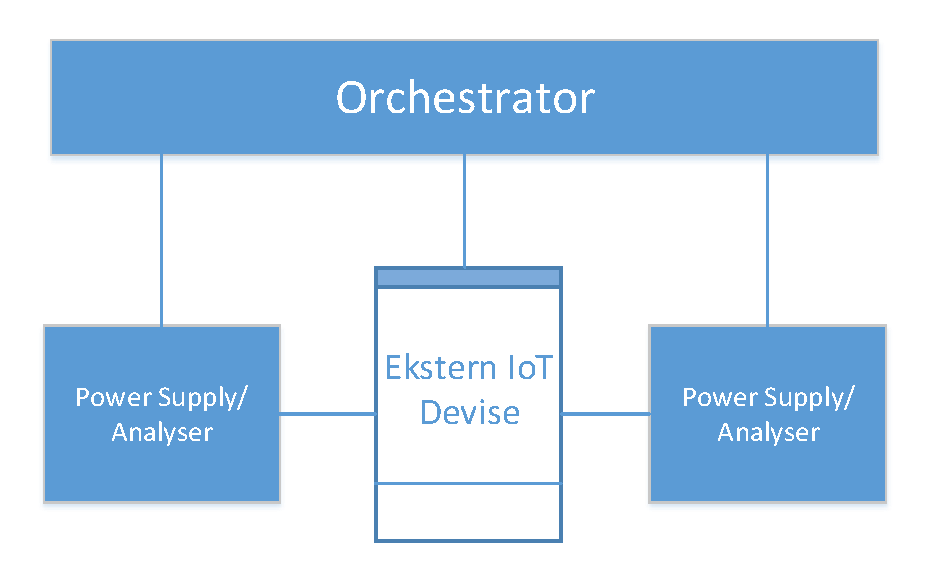
\includegraphics[width=0.5\textwidth]{figures/IPE_test_setup.pdf}
\begin{tikzpicture}
\draw  (-3.5,3) rectangle (6.5,2);
\draw  (-3.5,1) rectangle (-0.5,-1);
\draw  (0,1) rectangle (3,-1);
\draw  (3.5,1) rectangle (6.5,-1);
\node at (-2,0.25) {Power Supply Unit };
\node at (-2,-0.25) {and Analyser};
\node at (1.5,0) {DUT};
\node at (5,0) {UXM};
\node at (1.5,2.5) {Orchestrator};
\draw (-2,2) -- (-2,1);
\draw (1.5,2) -- (1.5,1);
\draw (5,2) -- (5,1);
\draw (-0.5,0) -- (0,0);
\draw(3,0) -- (3.5,0);
\end{tikzpicture}
\caption{Setup used to test for the power efficiency of the \gls{DUT}'s}
\label{fig:IPE_test_setup}
\end{figure}


As seen in \autoref{fig:IPE_test_setup}, an orchestrator, in this case \gls{TAP}, maintains the system. The orchestrator has a \gls{LAN} connection with the \gls{PSU} and the UXM and in this case a serial connection with the DUT. The \gls{PSU}s connection with the DUT is wires used to power on and analyse the power consumption of the device. It should be noted that the \gls{DUT} in question have two power inputs, one for the device power and one for the RF modem power, here only the modem is connected to the power analyser. The DUT is connected to the UXM using RF SMA cables.

\gls{TAP} is a software developed by Keysight Technologies which enables quick and easy access to the computers external connection. It also allows for C\# features to be used in the test design, meaning test steps can and has been designed to enable functionalities of the instruments. This includes for instance cell activation of the UXM and data collection from the PSU among other key functionalities, this couple with the ability to use loops, parallel test steps, serial com ports and batch scripts make this a very strong tool in designing, controlling and performing measurements. \citep{TAP} 

The \gls{PSU} is a N6705C DC Power Analyzer with the internal module TBD it has a range of TBD. When getting data from the PSU it can be done in a couple different ways, but here it is stored in the internal RAM of the PSU before download. This though has a limitation of 512.000 data points per capture. \citep{PSU}

The base station is a E7515A UXM Wireless Test Set from Keysight Technologies which is able to emulate, both LTE and NB-IoT conditions. It features most of the functionalities in the NB-IoT protocol until release 13. It has a multitude of changeable parameters with easy access through a SCPI interface. \citep{UXM}

The initial settings of each component in the system can be seen in \autoref{tab:setup_parameters}.

\begin{table}[H]
\captionsetup{belowskip=0em}
\noindent
\centering
%\resizebox{!}{0.5\textheight}{
\begin{minipage}[t]{0.48\textwidth}
\begin{tabular}{|p{4cm}|p{2cm}|}
\hline
\multicolumn{2}{|c|}{\textbf{Power Supply/Analyser}}                         \\ \hline
Enable             & Off            \\ \hline
Volt               & 3.6 V          \\ \hline
Ampere             & 2.5 A          \\ \hline
Sample interval	   & 100 $\mu$s		\\ \hline
\multicolumn{2}{c}{}\\ \hline
\multicolumn{2}{|c|}{\textbf{Ekstern IoT device}}                            \\ \hline
Enable             & Off            \\ \hline
DL\_EARFCN         & 6240           \\ \hline
\end{tabular}
%\caption{Initial values of the parameters in the emulator.}
\end{minipage}% 
\hfill
\begin{minipage}[t]{0.48\textwidth}
\begin{tabular}{|p{4cm}|p{2cm}|} \hline
\multicolumn{2}{|c|}{\textbf{UXM \gls{BSE}}} \\ \hline
Cell type			 & NB-IoT         \\ \hline
Number of cells		 & 1              \\ \hline
Operation mode		 & Standalone     \\ \hline
Host cell DL\_EARFCN & 6240           \\ \hline
PRB offset			 & 0	          \\ \hline
Cell ID				 & 0              \\ \hline
Tx power			 & -80 dB/per 15 kHz \\ \hline
Repetition NPDSCH	 & 1	          \\ \hline
Max Repetition NPDCCH & 4	          \\ \hline
Repetition NPUSCH	 & 1	          \\ \hline
Repetition NPRACH	 & 1	          \\ \hline
CP format			 & Normal         \\ \hline
$P_{TX}$				 & 23 dBm         \\ \hline
MAC padding DL		 & off       	  \\ \hline
MAC padding UL		 & off       	  \\ \hline
\end{tabular}
%\caption{Initial values of the parameters in the emulator.}
%\label{tab:setup_parameters}
\end{minipage}
\caption{Initial values of the parameters in the emulator.}
\label{tab:setup_parameters}
\end{table}

The procedures to measure the different elements can be in \appref{app:test_procedures}. When the data is procured the energy, power and time is needed for different parts of the measurement and is calculated respectively as:

\begin{align}
E &= \int_{A_{start}}^{A_{end}} f(x) dx \label{eq:energy}\\
P &= \mathbf{E}(f(x)) \quad for \, A_{start} \leq x \leq A_{end} \label{eq:power} \\
T &=  A_{end} - A_{start} \label{eq:time}\\
\end{align}
\begin{where}
\va{$E$}{is the energy of area A}{J}
\va{$P$}{is the average power consumption of area A}{W} 
\va{$T$}{is the duration of area A}{s}
\va{$\mathbf{E}$(•)}{is the mean function}{1}
\va{f(x)}{is the data point at time x}{W}
\va{$A_{start}$}{is the start time of area A}{s}
\va{$A_{end}$}{is the end time of area A}{s}
\end{where}

Four different kinds of idle mode exist for a NB-IoT device: \gls{cDRX}, \gls{DRX}, \gls{eDRX} and \gls{PSM}. It is chosen not to look into \gls{cDRX} due to an assumption of the device transmitting its data quickly and then going into deep sleep. 

When the device is in idle mode most parameters lose their influence entirely. Because of this a whole new set of parameters should be considered. For the \gls{DRX} case the cycle period is important, while for \gls{eDRX} however a few parameter more should be considered such as the repetition of the DRX cycle and the eDRX cycle period. For \gls{PSM} its is also the DRX cycle period as well as the repetition of the DRX cycle as well as the PSM cycle time. This can be summed up to two different types of parameters: period lengths and repetition numbers. It is assumed that both of these parameters have a proportional relation to the energy consumption of the idle modes, this means that only a single instance of the power consumption is needed for these different idle modes to extrapolate from.

Because of this an extra set of parameters need to be defined for the UXM, as can be seen in \autoref{tab:UXM_idle_values}.

\begin{table}[H]
\centering
\begin{tabular}{|c|c|} \hline
\multicolumn{2}{|c|}{\textbf{DRX}}  	 \\ \hline
Long DRX cycle     	& 1024 subframes 	 \\ \hline
onDuration Timer   	& 4 NPDCCH subframes \\ \hline
Retransmission Timer & 2 NPDCCH subframes \\ \hline
Inactivity Timer   	& 8 NPDCCH subframes \\ \hline
DRX Start Offset   	& 0              	 \\ \hline
drx-ULRetransmissionTimer & 0       	 \\ \hline
\multicolumn{2}{|c|}{\textbf{eDRX}} 	 \\ \hline
Idle eDRX State		& Off				 \\ \hline
\gls{PTW}			& 5120 subframes 	 \\ \hline
Idle eDRX Cycle     & 20480 subframes	 \\ \hline
\multicolumn{2}{|c|}{\textbf{PSM}}  	 \\ \hline
Power Saving Mode	& Off				 \\ \hline
T3324 (DRX period)	& 10 s    			 \\ \hline
T3412 (PSM period)	& 10 s		  		 \\ \hline
\end{tabular}
\caption{Specific parameter used to measure device idle power}
\label{tab:UXM_idle_values}
\end{table}




%\subsubsection{Device Power Consumption}
%
%To measure the device power, the power input to the device is used in the setup. The test is performed using the following procedure:
%
%\textbf{Test Procedure}
%\vspace{-1.5em}
%\begin{enumerate}
%\item Setup the \gls{DUT} as shown on \autoref{fig:IPE_test_setup}
%\item Put in settings as described in \autoref{tab:setup_parameters} and \autoref{tab:UXM_initial_values} 
%\item Turn on power supply 
%\item Measure power output over 2 min
%\item Save measurements as "<device>\_Power\_consumption"
%\item Turn off power supply
%\item Change to next \gls{DUT}
%\item Repeat step 1-7 for all \gls{DUT}s.
%\end{enumerate}
%
%\textbf{Results}\\
%\begin{table}[H]
%\centering
%\begin{tabular}{|c|c|c|c|}\hline
%\textbf{Device}	& Quectel	& Telit & Ublox \\ \hline
%$\mathbf{P_{device}}$	& & & \\ \hline
%\end{tabular}
%\caption{Average power consumption of the \gls{DUT}s}
%\label{tab:device_power_results}
%\end{table}

\section{Energy to Connect and Disconnect the DUT to the Cell} \label{sec:performance_attach}

First step is to get an overview of the measurements, to do this an example of the raw data from a measurement is presented in \autoref{fig:Attach_raw}.

\tikzsetnextfilename{Attach_raw}
\begin{figure}[H]
\centering
\begin{minipage}[tbp]{0.58\textwidth}
\resizebox{\textwidth}{!}{
% This file was created by matlab2tikz.
%
%The latest updates can be retrieved from
%  http://www.mathworks.com/matlabcentral/fileexchange/22022-matlab2tikz-matlab2tikz
%where you can also make suggestions and rate matlab2tikz.
%
\definecolor{mycolor1}{rgb}{0.00000,0.44700,0.74100}%
%
\begin{tikzpicture}
\begin{axis}[%
width=\textwidth,
height=0.66\textwidth,
at={(0.758in,0.481in)},
scale only axis,
xmin=0,
xmax=16,
xlabel={Time [s]},
ymin=-0.1,
ymax=0.8,
ylabel={Power Consumption [W]},
axis background/.style={fill=white}
]
\addplot [color=mycolor1,only marks,mark=*,mark options={solid},forget plot]
  table[row sep=crcr]{%
0	-0.00027465822\\
0.007168	-0.000137329092\\
0.014336	0\\
0.021504	-0.000137329092\\
0.028672	-0.000320435136\\
0.03584	-0.000160217568\\
0.043008	-0.000137329092\\
0.050176	-0.000137329092\\
0.057344	-4.5776088e-05\\
0.064512	-9.1553004e-05\\
0.07168	0.000205992828\\
0.078848	-0.00036621108\\
0.086016	-0.00027465822\\
0.093184	-0.000183106044\\
0.100352	-0.000251770572\\
0.10752	-0.00041198724\\
0.114688	-0.00057220488\\
0.121856	-0.000228882132\\
0.129024	-0.00041198724\\
0.136192	-4.5776088e-05\\
0.14336	4.5776088e-05\\
0.150528	-0.00059509332\\
0.157696	-0.00054931644\\
0.164864	-0.0006637572\\
0.172032	-0.000228882132\\
0.1792	-0.000114440652\\
0.186368	0.00034332192\\
0.193536	-0.000320435136\\
0.200704	-0.00018310518\\
0.207872	-4.5776916e-05\\
0.21504	-0.000183106044\\
0.222208	-0.00057220488\\
0.229376	0.000251769744\\
0.236544	-0.00048065184\\
0.243712	6.8664564e-05\\
0.25088	-0.00052642872\\
0.258048	-0.000228882132\\
0.265216	-2.28884616e-05\\
0.272384	-0.00043487568\\
0.279552	-0.000160217568\\
0.28672	-0.0004577634\\
0.293888	0.00018310518\\
0.301056	-0.000160217568\\
0.308224	-0.00054931644\\
0.315392	-0.000160217568\\
0.32256	-0.000205993656\\
0.329728	-4.5776088e-05\\
0.336896	-0.000228882132\\
0.344064	-0.000114440652\\
0.351232	-0.000160217568\\
0.3584	-0.000160217568\\
0.365568	-0.00045776412\\
0.372736	-0.00036621108\\
0.379904	-0.00061798104\\
0.387072	-0.00070953408\\
0.39424	-0.00043487568\\
0.401408	-9.1553004e-05\\
0.408576	-0.00027465822\\
0.415744	0\\
0.422912	-0.000160217568\\
0.43008	-0.000251769744\\
0.437248	-0.00057220488\\
0.444416	-0.00041198724\\
0.451584	-0.000160217568\\
0.458752	-0.000183106044\\
0.46592	-6.8664564e-05\\
0.473088	4.5776088e-05\\
0.480256	-0.000251769744\\
0.487424	0.0003890988\\
0.494592	-0.00018310518\\
0.50176	-0.000320434308\\
0.508928	2.28876264e-05\\
0.516096	-0.00043487568\\
0.523264	-0.00041198724\\
0.530432	-9.1553004e-05\\
0.5376	0.00016021674\\
0.544768	-0.00018310518\\
0.551936	-0.00029754666\\
0.559104	-0.0006637572\\
0.566272	0\\
0.57344	0.000114440652\\
0.580608	-0.000160217568\\
0.587776	-0.000160217568\\
0.594944	-0.0006637572\\
0.602112	-0.000183106044\\
0.60928	-0.00057220488\\
0.616448	-0.000137329092\\
0.623616	-0.000526428\\
0.630784	0.00018310518\\
0.637952	-6.8664564e-05\\
0.64512	9.1552176e-05\\
0.652288	0\\
0.659456	2.28876264e-05\\
0.666624	-0.000251770572\\
0.673792	-0.000343322748\\
0.68096	-0.0006637572\\
0.688128	-0.000160217568\\
0.695296	-0.000228882132\\
0.702464	0\\
0.709632	-0.0004577634\\
0.7168	-0.00029754666\\
0.723968	0.000114440652\\
0.731136	-0.0004577634\\
0.738304	-0.000343322748\\
0.745472	-0.000137329092\\
0.75264	4.5776088e-05\\
0.759808	0.000205993656\\
0.766976	-0.000343322748\\
0.774144	-0.000343322748\\
0.781312	4.5776088e-05\\
0.78848	-0.00029754666\\
0.795648	-0.00027465822\\
0.802816	4.5776088e-05\\
0.809984	-0.00041198724\\
0.817152	-9.1553004e-05\\
0.82432	2.28876264e-05\\
0.831488	-0.000228882132\\
0.838656	-0.0003890988\\
0.845824	-2.28884616e-05\\
0.852992	-0.000228882132\\
0.86016	-4.5776916e-05\\
0.867328	-0.000160217568\\
0.874496	-0.0004577634\\
0.881664	-0.000137329092\\
0.888832	-0.00029754666\\
0.896	0.00016021674\\
0.903168	-0.000343322748\\
0.910336	-0.0005950926\\
0.917504	-0.00027465822\\
0.924672	-0.00057220488\\
0.93184	-0.000114440652\\
0.939008	-4.5776916e-05\\
0.946176	9.1552176e-05\\
0.953344	0\\
0.960512	6.8664564e-05\\
0.96768	6.86637e-05\\
0.974848	-0.000160217568\\
0.982016	-4.5776088e-05\\
0.989184	-0.00054931644\\
0.996352	-0.00011444148\\
1.00352	-0.00050354028\\
1.010688	-0.000526428\\
1.017856	0.000137329092\\
1.025024	-0.000205993656\\
1.032192	0\\
1.03936	-0.00029754666\\
1.046528	-0.0005950926\\
1.053696	-0.00061798104\\
1.060864	-0.000205993656\\
1.068032	-0.000160217568\\
1.0752	-0.00011444148\\
1.082368	-0.000297545832\\
1.089536	-0.000343322748\\
1.096704	-0.0003890988\\
1.103872	-0.0003890988\\
1.11104	-0.00068664564\\
1.118208	0.00018310518\\
1.125376	0\\
1.132544	6.8664564e-05\\
1.139712	6.86637e-05\\
1.14688	-0.00036621108\\
1.154048	-0.00054931644\\
1.161216	-0.000343322748\\
1.168384	-0.000137329092\\
1.175552	-0.000228882132\\
1.18272	-0.00054931644\\
1.189888	-0.00068664564\\
1.197056	-0.00011444148\\
1.204224	-6.8664564e-05\\
1.211392	-0.00036621108\\
1.21856	-0.000343322748\\
1.225728	-0.00011444148\\
1.232896	-0.00018310518\\
1.240064	-0.000320435136\\
1.247232	-0.00027465822\\
1.2544	-0.000320434308\\
1.261568	0\\
1.268736	-0.000251770572\\
1.275904	-0.00027465822\\
1.283072	-0.00061798104\\
1.29024	0.0138244608\\
1.297408	0.0141448968\\
1.304576	0.0188598636\\
1.311744	0.0189056376\\
1.318912	0.023666382\\
1.32608	0.01966095\\
1.333248	0.0197753904\\
1.340416	0.104026788\\
1.347584	0.102653496\\
1.354752	0.102745044\\
1.36192	0.103019724\\
1.369088	0.102127068\\
1.376256	0.101989728\\
1.383424	0.103042584\\
1.390592	0.101966868\\
1.39776	0.101989728\\
1.404928	0.102287304\\
1.412096	0.104209884\\
1.419264	0.103248576\\
1.426432	0.103820796\\
1.4336	0.103729248\\
1.440768	0.104026788\\
1.447936	0.1036377\\
1.455104	0.103294368\\
1.462272	0.104301468\\
1.46944	0.105857856\\
1.476608	0.108352656\\
1.483776	0.105789168\\
1.490944	0.106361388\\
1.498112	0.105880752\\
1.50528	0.10583496\\
1.512448	0.106155396\\
1.519616	0.106979364\\
1.526784	0.10949706\\
1.533952	0.111213684\\
1.54112	0.108489996\\
1.548288	0.109909044\\
1.555456	0.110389716\\
1.562624	0.112197888\\
1.569792	0.11592864\\
1.57696	0.112907412\\
1.584128	0.11357118\\
1.591296	0.1131363\\
1.598464	0.11286162\\
1.605632	0.112472532\\
1.6128	0.115219116\\
1.619968	0.115173324\\
1.627136	0.114784236\\
1.634304	0.116249076\\
1.641472	0.116134632\\
1.64864	0.116455068\\
1.655808	0.11606598\\
1.662976	0.116546616\\
1.670144	0.118583676\\
1.677312	0.119773872\\
1.68448	0.119178756\\
1.691648	0.120826728\\
1.698816	0.12119292\\
1.705984	0.123046884\\
1.713152	0.123847956\\
1.72032	0.123870852\\
1.727488	0.124900812\\
1.734656	0.126319896\\
1.741824	0.12718962\\
1.748992	0.128585808\\
1.75616	0.128036484\\
1.763328	0.127967832\\
1.770496	0.128585808\\
1.777664	0.145133964\\
1.784832	0.1537857\\
1.792	0.153579708\\
1.799168	0.153396612\\
1.806336	0.1537857\\
1.813504	0.153099072\\
1.820672	0.15319062\\
1.82784	0.153396612\\
1.835008	0.151496892\\
1.842176	0.153327924\\
1.849344	0.0260238636\\
1.856512	0.0298919664\\
1.86368	0.0287704476\\
1.870848	0.0258865344\\
1.878016	0.028930662\\
1.885184	0.036781308\\
1.892352	0.0302352876\\
1.89952	0.037033092\\
1.906688	0.036186228\\
1.913856	0.0296630856\\
1.921024	0.0331649784\\
1.928192	0.042068484\\
1.93536	0.047904984\\
1.942528	0.0323638884\\
1.949696	0.037078848\\
1.956864	0.076766976\\
1.964032	0.0332336412\\
1.9712	0.039550788\\
1.978368	0.043601976\\
1.985536	0.03609468\\
1.992704	0.03588867\\
1.999872	0.0334854108\\
2.00704	0.0326614356\\
2.014208	0.03872682\\
2.021376	0.0359573364\\
2.028544	0.03362274\\
2.035712	0.044036856\\
2.04288	0.0303955056\\
2.050048	0.0336456288\\
2.057216	0.0338745096\\
2.064384	0.0335540772\\
2.071552	0.043395984\\
2.07872	0.038795472\\
2.085888	0.03362274\\
2.093056	0.036483768\\
2.100224	0.030830382\\
2.107392	0.0330047604\\
2.11456	0.0351333612\\
2.121728	0.0334396368\\
2.128896	0.0325927728\\
2.136064	0.034103394\\
2.143232	0.0331420896\\
2.1504	0.03552246\\
2.157568	0.0335998512\\
2.164736	0.0337371804\\
2.171904	0.0333938592\\
2.179072	0.03325653\\
2.18624	0.0359802252\\
2.193408	0.033782958\\
2.200576	0.0332336412\\
2.207744	0.0330505344\\
2.214912	0.033576966\\
2.22208	0.03588867\\
2.229248	0.0330505344\\
2.236416	0.033576966\\
2.243584	0.0338745096\\
2.250752	0.041152968\\
2.25792	0.0339660648\\
2.265088	0.051269544\\
2.272256	0.044403084\\
2.279424	0.031402584\\
2.286592	0.038314836\\
2.29376	0.0336456288\\
2.300928	0.038658132\\
2.308096	0.03918456\\
2.315264	0.0352706904\\
2.322432	0.0335082996\\
2.3296	0.0336685176\\
2.336768	0.042137136\\
2.343936	0.0346755996\\
2.351104	0.042503364\\
2.358272	0.038818368\\
2.36544	0.0344238264\\
2.372608	0.0319290156\\
2.379776	0.037147536\\
2.386944	0.0300292956\\
2.394112	0.0344924892\\
2.40128	0.0334396368\\
2.408448	0.0336456288\\
2.415616	0.0326614356\\
2.422784	0.0337142952\\
2.429952	0.0308761596\\
2.43712	0.03289032\\
2.444288	0.039367656\\
2.451456	0.03325653\\
2.458624	0.0337142952\\
2.465792	0.03362274\\
2.47296	0.048568716\\
2.480128	0.0314712504\\
2.487296	0.044471736\\
2.494464	0.0350189208\\
2.501632	0.036506664\\
2.5088	0.0321578964\\
2.515968	0.0257949828\\
2.523136	0.0204162588\\
2.530304	0.0205306992\\
2.537472	0.020553588\\
2.54464	0.0205078104\\
2.551808	0.0208053576\\
2.558976	0.0205306992\\
2.566144	0.0203704812\\
2.573312	0.0203247072\\
2.58048	0.02039337\\
2.587648	0.0206222508\\
2.594816	0.020553588\\
2.601984	0.020874024\\
2.609152	0.0201187116\\
2.61632	0.020553588\\
2.623488	0.0205078104\\
2.630656	0.0204162588\\
2.637824	0.0205306992\\
2.644992	0.0205764768\\
2.65216	0.0207366948\\
2.659328	0.0204162588\\
2.666496	0.0201644892\\
2.673664	0.0207366948\\
2.680832	0.0208511352\\
2.688	0.0205764768\\
2.695168	0.0206909172\\
2.702336	0.02039337\\
2.709504	0.020874024\\
2.716672	0.0205306992\\
2.72384	0.0202789296\\
2.731008	0.0207824688\\
2.738176	0.0205306992\\
2.745344	0.0209426868\\
2.752512	0.0203704812\\
2.75968	0.0204620364\\
2.766848	0.020347596\\
2.774016	0.020874024\\
2.781184	0.0204620364\\
2.788352	0.0246505752\\
2.79552	0.02039337\\
2.802688	0.0204620364\\
2.809856	0.0210113532\\
2.817024	0.020187378\\
2.824192	0.0206680284\\
2.83136	0.0205993656\\
2.838528	0.020553588\\
2.845696	0.0203018184\\
2.852864	0.0205993656\\
2.860032	0.0206222544\\
2.8672	0.020713806\\
2.874368	0.0203475924\\
2.881536	0.0208053576\\
2.888704	0.0203247072\\
2.895872	0.0201644892\\
2.90304	0.0205764768\\
2.910208	0.0208282464\\
2.917376	0.0208053576\\
2.924544	0.0207595836\\
2.931712	0.0205078104\\
2.93888	0.0204162588\\
2.946048	0.020553588\\
2.953216	0.0204620364\\
2.960384	0.0206222508\\
2.967552	0.0205306992\\
2.97472	0.0205993656\\
2.981888	0.0204620364\\
2.989056	0.0207366948\\
2.996224	0.020347596\\
3.003392	0.0204849252\\
3.01056	0.0204162588\\
3.017728	0.0203475924\\
3.024896	0.0203018184\\
3.032064	0.0202560408\\
3.039232	0.0204620364\\
3.0464	0.020713806\\
3.053568	0.0204162588\\
3.060736	0.0203018184\\
3.067904	0.0208969128\\
3.075072	0.020553588\\
3.08224	0.0205306992\\
3.089408	0.0204849252\\
3.096576	0.02039337\\
3.103744	0.0204162588\\
3.110912	0.0201416004\\
3.11808	0.0206909172\\
3.125248	0.0205764768\\
3.132416	0.0203247072\\
3.139584	0.020347596\\
3.146752	0.0207595836\\
3.15392	0.0200500488\\
3.161088	0.020713806\\
3.168256	0.0200042712\\
3.175424	0.0203247072\\
3.182592	0.0205764768\\
3.18976	0.0202560408\\
3.196928	0.020713806\\
3.204096	0.0208053576\\
3.211264	0.020187378\\
3.218432	0.0204391476\\
3.2256	0.0205306992\\
3.232768	0.02039337\\
3.239936	0.0203247072\\
3.247104	0.0207366948\\
3.254272	0.020713806\\
3.26144	0.020553588\\
3.268608	0.0203475924\\
3.275776	0.0203247072\\
3.282944	0.020072934\\
3.290112	0.0204849216\\
3.29728	0.0205993656\\
3.304448	0.0206451396\\
3.311616	0.0208053576\\
3.318784	0.024513246\\
3.325952	0.0209655756\\
3.33312	0.0205764768\\
3.340288	0.0202102632\\
3.347456	0.0200729376\\
3.354624	0.0202102668\\
3.361792	0.0203247072\\
3.36896	0.0202102668\\
3.376128	0.0206451396\\
3.383296	0.02002716\\
3.390464	0.0204620364\\
3.397632	0.0208282464\\
3.4048	0.0204391476\\
3.411968	0.020713806\\
3.419136	0.020233152\\
3.426304	0.0207595836\\
3.433472	0.0203704812\\
3.44064	0.0203704812\\
3.447808	0.0206909172\\
3.454976	0.0207824688\\
3.462144	0.020347596\\
3.469312	0.0204849252\\
3.47648	0.0205993656\\
3.483648	0.020553588\\
3.490816	0.0208053576\\
3.497984	0.0204162588\\
3.505152	0.0206680284\\
3.51232	0.0204162588\\
3.519488	0.0199584936\\
3.526656	0.0200729376\\
3.533824	0.0206222544\\
3.540992	0.02039337\\
3.54816	0.0205078104\\
3.555328	0.0204391476\\
3.562496	0.0204849216\\
3.569664	0.0209655756\\
3.576832	0.0204391476\\
3.584	0.0202789296\\
3.591168	0.020233152\\
3.598336	0.0204620364\\
3.605504	0.020874024\\
3.612672	0.020713806\\
3.61984	0.020713806\\
3.627008	0.0206909172\\
3.634176	0.0202789296\\
3.641344	0.0205306992\\
3.648512	0.0203018184\\
3.65568	0.0205306992\\
3.662848	0.0204391476\\
3.670016	0.0208511352\\
3.677184	0.0204620364\\
3.684352	0.0202789296\\
3.69152	0.0205993656\\
3.698688	0.0203475924\\
3.705856	0.0201187116\\
3.713024	0.0200729376\\
3.720192	0.0206680284\\
3.72736	0.0205764768\\
3.734528	0.0207824688\\
3.741696	0.020874024\\
3.748864	0.0204849216\\
3.756032	0.0201644892\\
3.7632	0.0202102668\\
3.770368	0.0208969128\\
3.777536	0.0204391476\\
3.784704	0.0200958228\\
3.791872	0.0199356084\\
3.79904	0.0204849252\\
3.806208	0.0232086168\\
3.813376	0.024513246\\
3.820544	0.0223388676\\
3.827712	0.020233152\\
3.83488	0.020553588\\
3.842048	0.0206222544\\
3.849216	0.0205306992\\
3.856384	0.02002716\\
3.863552	0.0206222544\\
3.87072	0.0202560408\\
3.877888	0.0202789296\\
3.885056	0.0205078104\\
3.892224	0.020187378\\
3.899392	0.0203018184\\
3.90656	0.0206451396\\
3.913728	0.02039337\\
3.920896	0.0202560408\\
3.928064	0.020919798\\
3.935232	0.0206222544\\
3.9424	0.0206909172\\
3.949568	0.0204620364\\
3.956736	0.0204162588\\
3.963904	0.020233152\\
3.971072	0.020553588\\
3.97824	0.0202560408\\
3.985408	0.0204391476\\
3.992576	0.0203247072\\
3.999744	0.0204391476\\
4.006912	0.020553588\\
4.01408	0.0207366948\\
4.021248	0.0205306992\\
4.028416	0.0204391476\\
4.035584	0.0203704812\\
4.042752	0.0203018184\\
4.04992	0.0201416004\\
4.057088	0.020713806\\
4.064256	0.020187378\\
4.071424	0.0204849216\\
4.078592	0.020187378\\
4.08576	0.0202102668\\
4.092928	0.0205764768\\
4.100096	0.0205993656\\
4.107264	0.0205764768\\
4.114432	0.0208053576\\
4.1216	0.0201416004\\
4.128768	0.0203247072\\
4.135936	0.0208282464\\
4.143104	0.0205993656\\
4.150272	0.0210571272\\
4.15744	0.0202102668\\
4.164608	0.0205306992\\
4.171776	0.0206909172\\
4.178944	0.0211715676\\
4.186112	0.020553588\\
4.19328	0.0206680284\\
4.200448	0.020553588\\
4.207616	0.0206680284\\
4.214784	0.020187378\\
4.221952	0.0204620364\\
4.22912	0.0197753904\\
4.236288	0.0206222544\\
4.243456	0.0205993656\\
4.250624	0.02039337\\
4.257792	0.0205764768\\
4.26496	0.0208511352\\
4.272128	0.0206222544\\
4.279296	0.02002716\\
4.286464	0.0207595836\\
4.293632	0.0204162588\\
4.3008	0.0206451396\\
4.307968	0.0205993656\\
4.315136	0.028244016\\
4.322304	0.200042712\\
4.329472	0.22570038\\
4.33664	0.243667584\\
4.343808	0.21283722\\
4.350976	0.254035944\\
4.358144	0.233001684\\
4.365312	0.245521512\\
4.37248	0.22190094\\
4.379648	0.253761264\\
4.386816	0.24895476\\
4.393984	0.246894804\\
4.401152	0.0249481188\\
4.40832	0.020553588\\
4.415488	0.149894712\\
4.422656	0.19953918\\
4.429824	0.232017516\\
4.436992	0.152389512\\
4.44416	0.14955138\\
4.451328	0.201919536\\
4.458496	0.155158992\\
4.465664	0.155754072\\
4.472832	0.200958264\\
4.48	0.19983672\\
4.487168	0.0242843616\\
4.494336	0.153282168\\
4.501504	0.201553344\\
4.508672	0.152458164\\
4.51584	0.159553512\\
4.523008	0.201095568\\
4.530176	0.197937\\
4.537344	0.151908876\\
4.544512	0.160995492\\
4.55168	0.201416004\\
4.558848	0.150627132\\
4.566016	0.0281753532\\
4.573184	0.153671256\\
4.580352	0.201782232\\
4.58752	0.155342088\\
4.594688	0.15319062\\
4.601856	0.200386044\\
4.609024	0.201347352\\
4.616192	0.15541074\\
4.62336	0.156967164\\
4.630528	0.201507552\\
4.637696	0.151062012\\
4.644864	0.0321807852\\
4.652032	0.0286331184\\
4.6592	0.0251998884\\
4.666368	0.0207366948\\
4.673536	0.0247421268\\
4.680704	0.020233152\\
4.687872	0.02039337\\
4.69504	0.024513246\\
4.702208	0.0201416004\\
4.709376	0.219451896\\
4.716544	0.024765012\\
4.723712	0.0205764768\\
4.73088	0.202812192\\
4.738048	0.0247879044\\
4.745216	0.0208969128\\
4.752384	0.0208053576\\
4.759552	0.0202789296\\
4.76672	0.0206680284\\
4.773888	0.02039337\\
4.781056	0.0206222544\\
4.788224	0.0207366948\\
4.795392	0.0206222508\\
4.80256	0.149734476\\
4.809728	0.149322492\\
4.816896	0.14984892\\
4.824064	0.153831456\\
4.831232	0.2372589\\
4.8384	0.028083798\\
4.845568	0.0246963492\\
4.852736	0.02419281\\
4.859904	0.0205306992\\
4.867072	0.0204849252\\
4.87424	0.0248336784\\
4.881408	0.0208511352\\
4.888576	0.020713806\\
4.895744	0.0246963492\\
4.902912	0.0204620364\\
4.91008	0.208671552\\
4.917248	0.0247421268\\
4.924416	0.020233152\\
4.931584	0.0205993656\\
4.938752	0.0211715676\\
4.94592	0.0205764768\\
4.953088	0.0205306992\\
4.960256	0.0203018184\\
4.967424	0.150489792\\
4.974592	0.15232086\\
4.98176	0.150260904\\
4.988928	0.150398244\\
4.996096	0.150306696\\
5.003264	0.150100704\\
5.010432	0.1502838\\
5.0176	0.150329592\\
5.024768	0.221717844\\
5.031936	0.150970464\\
5.039104	0.150489792\\
5.046272	0.151268004\\
5.05344	0.150352488\\
5.060608	0.151359552\\
5.067776	0.14998626\\
5.074944	0.151657092\\
5.082112	0.149528484\\
5.08928	0.151794432\\
5.096448	0.149734476\\
5.103616	0.15188598\\
5.110784	0.0278091432\\
5.117952	0.0489807\\
5.12512	0.153259272\\
5.132288	0.249572736\\
5.139456	0.0277862544\\
5.146624	0.0290222172\\
5.153792	0.0274429296\\
5.16096	0.0280609128\\
5.168128	0.024513246\\
5.175296	0.0252914436\\
5.182464	0.0249481188\\
5.189632	0.0333709704\\
5.1968	0.0303268428\\
5.203968	0.0296630856\\
5.211136	0.274566636\\
5.218304	0.246734604\\
5.225472	0.155136096\\
5.23264	0.221008284\\
5.239808	0.024879456\\
5.246976	0.0249023412\\
5.254144	0.207778932\\
5.261312	0.050148\\
5.26848	0.214508052\\
5.275648	0.213203448\\
5.282816	0.0295257564\\
5.289984	0.44702892\\
5.297152	0.4543992\\
5.30432	0.44274888\\
5.311488	0.4561614\\
5.318656	0.44068896\\
5.325824	0.151176456\\
5.332992	0.201942432\\
5.34016	0.250602696\\
5.347328	0.0230255136\\
5.354496	0.0205306992\\
5.361664	0.0205764768\\
5.368832	0.0204391476\\
5.376	0.131629932\\
5.383168	0.224876376\\
5.390336	0.0251312256\\
5.397504	0.219383244\\
5.404672	0.0239181516\\
5.41184	0.030670164\\
5.419008	0.71953596\\
5.426176	0.72981252\\
5.433344	0.254631024\\
5.440512	0.15158844\\
5.44768	0.218284596\\
5.454848	0.21416472\\
5.462016	0.216911304\\
5.469184	0.198188784\\
5.476352	0.0205078104\\
5.48352	0.0205306992\\
5.490688	0.0206222508\\
5.497856	0.020553588\\
5.505024	0.020553588\\
5.512192	0.203590404\\
5.51936	0.0284271228\\
5.526528	0.71548452\\
5.533696	0.73143756\\
5.540864	0.7099686\\
5.548032	0.72892008\\
5.5552	0.70976268\\
5.562368	0.73123164\\
5.569536	0.71083836\\
5.576704	0.72988128\\
5.583872	0.71276076\\
5.59104	0.0250167816\\
5.598208	0.254241936\\
5.605376	0.0242843616\\
5.612544	0.0203704812\\
5.619712	0.0208969128\\
5.62688	0.0204391476\\
5.634048	0.209701548\\
5.641216	0.215057376\\
5.648384	0.0272827152\\
5.655552	0.72972108\\
5.66272	0.7143174\\
5.669888	0.72569268\\
5.677056	0.709236\\
5.684224	0.72921744\\
5.691392	0.71058636\\
5.69856	0.72985824\\
5.705728	0.70925904\\
5.712896	0.72990432\\
5.720064	0.204917904\\
5.727232	0.0245819088\\
5.7344	0.0204391476\\
5.741568	0.0202789296\\
5.748736	0.020553588\\
5.755904	0.0202789296\\
5.763072	0.020347596\\
5.77024	0.0204849252\\
5.777408	0.205810524\\
5.784576	0.197364816\\
5.791744	0.208534248\\
5.798912	0.213386544\\
5.80608	0.0312652548\\
5.813248	0.72809604\\
5.820416	0.72649368\\
5.827584	0.0285873408\\
5.834752	0.218719476\\
5.84192	0.153579708\\
5.849088	0.16181946\\
5.856256	0.213203448\\
5.863424	0.249435396\\
5.870592	0.157241808\\
5.87776	0.039253248\\
5.884928	0.0331192008\\
5.892096	0.216224676\\
5.899264	0.258567804\\
5.906432	0.230712876\\
5.9136	0.265663152\\
5.920768	0.172828692\\
5.927936	0.21196746\\
5.935104	0.268157952\\
5.942272	0.224601732\\
5.94944	0.168914808\\
5.956608	0.21986388\\
5.963776	0.238609296\\
5.970944	0.17191314\\
5.978112	0.209976192\\
5.98528	0.0334854108\\
5.992448	0.041770944\\
5.999616	0.043533324\\
6.006784	0.043373124\\
6.013952	0.0349731432\\
6.02112	0.20670318\\
6.028288	0.235450728\\
6.035456	0.161132796\\
6.042624	0.237464892\\
6.049792	0.223205544\\
6.05696	0.235656756\\
6.064128	0.208557108\\
6.071296	0.231445296\\
6.078464	0.227508552\\
6.085632	0.150581376\\
6.0928	0.20100402\\
6.099968	0.225082404\\
6.107136	0.197410572\\
6.114304	0.0249481188\\
6.121472	0.02039337\\
6.12864	0.0207595836\\
6.135808	0.0204391476\\
6.142976	0.0201644892\\
6.150144	0.151130664\\
6.157312	0.244239804\\
6.16448	0.149574276\\
6.171648	0.210227976\\
6.178816	0.215835552\\
6.185984	0.185485824\\
6.193152	0.253417968\\
6.20032	0.207206712\\
6.207488	0.22279356\\
6.214656	0.249435396\\
6.221824	0.224853516\\
6.228992	0.202995288\\
6.23616	0.202926636\\
6.243328	0.024513246\\
6.250496	0.0206222544\\
6.257664	0.0208511352\\
6.264832	0.0202560408\\
6.272	0.131446836\\
6.279168	0.22583772\\
6.286336	0.202239972\\
6.293504	0.221946696\\
6.300672	0.150260904\\
6.30784	0.21956634\\
6.315008	0.204849252\\
6.322176	0.22000122\\
6.329344	0.20803068\\
6.336512	0.214210512\\
6.34368	0.211257936\\
6.350848	0.1501236\\
6.358016	0.213912972\\
6.365184	0.0280151352\\
6.372352	0.0207366948\\
6.37952	0.0204162588\\
6.386688	0.0204162588\\
6.393856	0.0203018184\\
6.401024	0.0207366948\\
6.408192	0.0245361312\\
6.41536	0.223457328\\
6.422528	0.200798028\\
6.429696	0.147811896\\
6.436864	0.20070648\\
6.444032	0.225791928\\
6.4512	0.195350652\\
6.458368	0.248085036\\
6.465536	0.150833124\\
6.472704	0.223022448\\
6.479872	0.202857948\\
6.48704	0.15042114\\
6.494208	0.206085204\\
6.501376	0.217620828\\
6.508544	0.207344052\\
6.515712	0.21372984\\
6.52288	0.0246505752\\
6.530048	0.149574276\\
6.537216	0.216247536\\
6.544384	0.249755868\\
6.551552	0.217918404\\
6.55872	0.206886276\\
6.565888	0.151542648\\
6.573056	0.205169688\\
6.580224	0.225494388\\
6.587392	0.2039337\\
6.59456	0.22586058\\
6.601728	0.201782232\\
6.608896	0.254104596\\
6.616064	0.192695616\\
6.623232	0.0247879044\\
6.6304	0.0204162588\\
6.637568	0.0204391476\\
6.644736	0.0203247072\\
6.651904	0.0206222544\\
6.659072	0.201187116\\
6.66624	0.219406104\\
6.673408	0.245841984\\
6.680576	0.148338324\\
6.687744	0.207115164\\
6.694912	0.215515116\\
6.70208	0.205078104\\
6.709248	0.229248036\\
6.716416	0.21503448\\
6.723584	0.229980456\\
6.730752	0.151496892\\
6.73792	0.207778932\\
6.745088	0.151542648\\
6.752256	0.02455902\\
6.759424	0.0204162588\\
6.766592	0.02039337\\
6.77376	0.0207366948\\
6.780928	0.0209884644\\
6.788096	0.201210012\\
6.795264	0.215309124\\
6.802432	0.2419281\\
6.8096	0.151863084\\
6.816768	0.225173952\\
6.823936	0.201667788\\
6.831104	0.196723944\\
6.838272	0.207412704\\
6.84544	0.149963364\\
6.852608	0.204574572\\
6.859776	0.217323288\\
6.866944	0.206932068\\
6.874112	0.195991524\\
6.88128	0.0306472752\\
6.888448	0.282531708\\
6.895616	0.0248107896\\
6.902784	0.0204162588\\
6.909952	0.02039337\\
6.91712	0.19397736\\
6.924288	0.0274200444\\
6.931456	0.20553588\\
6.938624	0.212745672\\
6.945792	0.0310134888\\
6.95296	0.46089936\\
6.960128	0.4420854\\
6.967296	0.4585878\\
6.974464	0.43782804\\
6.981632	0.027717588\\
6.9888	0.200775132\\
6.995968	0.177406308\\
7.003136	0.256919832\\
7.010304	0.0212860116\\
7.017472	0.0211486824\\
7.02464	0.0204849252\\
7.031808	0.0206451396\\
7.038976	0.0203704812\\
7.046144	0.0206451396\\
7.053312	0.221054076\\
7.06048	0.149322492\\
7.067648	0.0280151352\\
7.074816	0.72404496\\
7.081984	0.72248832\\
7.089152	0.72246564\\
7.09632	0.71784216\\
7.103488	0.72447984\\
7.110656	0.71514144\\
7.117824	0.72576144\\
7.124992	0.71040348\\
7.13216	0.72846216\\
7.139328	0.206382744\\
7.146496	0.226203912\\
7.153664	0.201644892\\
7.160832	0.0249710076\\
7.168	0.132179256\\
7.175168	0.226203912\\
7.182336	0.0253601064\\
7.189504	0.1476288\\
7.196672	0.212470992\\
7.20384	0.0308990484\\
7.211008	0.72843948\\
7.218176	0.73599228\\
7.225344	0.0274429296\\
7.232512	0.242546076\\
7.23968	0.213455196\\
7.246848	0.218124396\\
7.254016	0.216407772\\
7.261184	0.199310292\\
7.268352	0.0247879044\\
7.27552	0.0277404768\\
7.282688	0.0309677112\\
7.289856	0.029617308\\
7.297024	0.230781564\\
7.304192	0.215538012\\
7.31136	0.22952268\\
7.318528	0.239524848\\
7.325696	0.150695784\\
7.332864	0.201782232\\
7.340032	0.226181016\\
7.3472	0.202766436\\
7.354368	0.225425736\\
7.361536	0.200958264\\
7.368704	0.223869312\\
7.375872	0.214416504\\
7.38304	0.22235868\\
7.390208	0.065071116\\
7.397376	0.0250625628\\
7.404544	0.0207824688\\
7.411712	0.0207824688\\
7.41888	0.0207595836\\
7.426048	0.13286592\\
7.433216	0.213340752\\
7.440384	0.190452564\\
7.447552	0.215423568\\
7.45472	0.208328256\\
7.461888	0.218559276\\
7.469056	0.2062683\\
7.476224	0.221992488\\
7.483392	0.20436858\\
7.49056	0.151039116\\
7.497728	0.202880844\\
7.504896	0.21503448\\
7.512064	0.201965328\\
7.519232	0.200180052\\
7.5264	0.0208053576\\
7.533568	0.0211029048\\
7.540736	0.0208053576\\
7.547904	0.0206909172\\
7.555072	0.200683584\\
7.56224	0.237762432\\
7.569408	0.16197966\\
7.576576	0.218719476\\
7.583744	0.205879212\\
7.590912	0.149803164\\
7.59808	0.254013048\\
7.605248	0.149894712\\
7.612416	0.212860116\\
7.619584	0.230575572\\
7.626752	0.215583804\\
7.63392	0.208785996\\
7.641088	0.195510852\\
7.648256	0.0242614728\\
7.655424	0.0206909172\\
7.662592	0.0206222544\\
7.66976	0.0206222544\\
7.676928	0.0208282464\\
7.684096	0.0203704812\\
7.691264	0.0206909172\\
7.698432	0.24179076\\
7.7056	0.149528484\\
7.712768	0.22586058\\
7.719936	0.200546244\\
7.727104	0.199928268\\
7.734272	0.206886276\\
7.74144	0.22263336\\
7.748608	0.203155524\\
7.755776	0.147880548\\
7.762944	0.151336656\\
7.770112	0.149917608\\
7.77728	0.2170944\\
7.784448	0.149528484\\
7.791616	0.211326588\\
7.798784	0.0280838016\\
7.805952	0.0205993656\\
7.81312	0.194457996\\
7.820288	0.219612096\\
7.827456	0.207344052\\
7.834624	0.221214276\\
7.841792	0.205284132\\
7.84896	0.223297128\\
7.856128	0.191390976\\
7.863296	0.229591368\\
7.870464	0.149871816\\
7.877632	0.247032144\\
7.8848	0.149894712\\
7.891968	0.226272564\\
7.899136	0.194503788\\
7.906304	0.0242843616\\
7.913472	0.0205078104\\
7.92064	0.0208282464\\
7.927808	0.0203018184\\
7.934976	0.0203018184\\
7.942144	0.20086668\\
7.949312	0.218353284\\
7.95648	0.207984924\\
7.963648	0.233184816\\
7.970816	0.15174864\\
7.977984	0.21256254\\
7.985152	0.15204618\\
7.99232	0.211280832\\
7.999488	0.21839904\\
8.006656	0.207458496\\
8.013824	0.220573404\\
8.020992	0.186195384\\
8.02816	0.25069428\\
8.035328	0.0242843616\\
8.042496	0.020874024\\
8.049664	0.0206451396\\
8.056832	0.0206451396\\
8.064	0.0204620364\\
8.071168	0.200546244\\
8.078336	0.200431836\\
8.085504	0.150306696\\
8.092672	0.205787664\\
8.09984	0.254470824\\
8.107008	0.202514652\\
8.114176	0.235267632\\
8.121344	0.206291196\\
8.128512	0.238151556\\
8.13568	0.148704516\\
8.142848	0.214988724\\
8.150016	0.151863084\\
8.157184	0.215263368\\
8.164352	0.0243759168\\
8.17152	0.0206222544\\
8.178688	0.0205764768\\
8.185856	0.0203018184\\
8.193024	0.22263336\\
8.200192	0.207481392\\
8.20736	0.224166852\\
8.214528	0.2395935\\
8.221696	0.224807724\\
8.228864	0.207092268\\
8.236032	0.193290696\\
8.2432	0.203018184\\
8.250368	0.150810228\\
8.257536	0.201095568\\
8.264704	0.147399912\\
8.271872	0.201164256\\
8.27904	0.224327088\\
8.286208	0.0246734604\\
8.293376	0.020553588\\
8.300544	0.0205078104\\
8.307712	0.0198898308\\
8.31488	0.0201416004\\
8.322048	0.030464172\\
8.329216	0.27321624\\
8.336384	0.0249710076\\
8.343552	0.232154856\\
8.35072	0.149711616\\
8.357888	0.216911304\\
8.365056	0.149894712\\
8.372224	0.22162626\\
8.379392	0.250900272\\
8.38656	0.223571772\\
8.393728	0.203521716\\
8.400896	0.214485156\\
8.408064	0.149734476\\
8.415232	0.230758632\\
8.4224	0.201805128\\
8.429568	0.188644392\\
8.436736	0.195259104\\
8.443904	0.0249252336\\
8.451072	0.1932678\\
8.45824	0.235908504\\
8.465408	0.154975896\\
8.472576	0.21986388\\
8.479744	0.0273742668\\
8.486912	0.205261236\\
8.49408	0.44709768\\
8.501248	0.45444492\\
8.508416	0.44561016\\
8.515584	0.45256788\\
8.522752	0.216842652\\
8.52992	0.149963364\\
8.537088	0.206062308\\
8.544256	0.0251083368\\
8.551424	0.0208511352\\
8.558592	0.0203247072\\
8.56576	0.0206909172\\
8.572928	0.0205306992\\
8.580096	0.203659056\\
8.587264	0.244514448\\
8.594432	0.0300979584\\
8.6016	0.7146378\\
8.608768	0.73457352\\
8.615936	0.70882416\\
8.623104	0.72889704\\
8.630272	0.70953372\\
8.63744	0.73075104\\
8.644608	0.70985412\\
8.651776	0.72990432\\
8.658944	0.7124634\\
8.666112	0.19324494\\
8.67328	0.024513246\\
8.680448	0.0209426868\\
8.687616	0.0202102668\\
8.694784	0.0207366948\\
8.701952	0.0208511352\\
8.70912	0.194915772\\
8.716288	0.2170944\\
8.723456	0.215698248\\
8.730624	0.150970464\\
8.737792	0.0276260364\\
8.74496	0.187293996\\
8.752128	0.7160112\\
8.759296	0.73287972\\
8.766464	0.209747304\\
8.773632	0.225379944\\
8.7808	0.149528484\\
8.787968	0.226615896\\
8.795136	0.193954464\\
8.802304	0.0248107896\\
8.809472	0.0201187116\\
8.81664	0.0205078104\\
8.823808	0.0202789296\\
8.830976	0.020187378\\
8.838144	0.198623664\\
8.845312	0.149757372\\
8.85248	0.205490124\\
8.859648	0.235427832\\
8.866816	0.20800782\\
8.873984	0.214096068\\
8.881152	0.203567508\\
8.88832	0.244926468\\
8.895488	0.149642928\\
8.902656	0.20919798\\
8.909824	0.151245108\\
8.916992	0.206909172\\
8.92416	0.198783864\\
8.931328	0.0209884644\\
8.938496	0.0201187116\\
8.945664	0.0206680284\\
8.952832	0.0202560408\\
8.96	0.0208053576\\
8.967168	0.0250625628\\
8.974336	0.204551712\\
8.981504	0.225105264\\
8.988672	0.200729376\\
8.99584	0.213935832\\
9.003008	0.201553344\\
9.010176	0.150398244\\
9.017344	0.203956596\\
9.024512	0.147743208\\
9.03168	0.205558776\\
9.038848	0.217712412\\
9.046016	0.151702884\\
9.053184	0.196632396\\
9.060352	0.212814324\\
9.06752	0.211578372\\
9.074688	0.214942932\\
9.081856	0.0248565672\\
9.089024	0.221397408\\
9.096192	0.194686884\\
9.10336	0.222175584\\
9.110528	0.150100704\\
9.117696	0.225952128\\
9.124864	0.150077808\\
9.132032	0.225631728\\
9.1392	0.20407104\\
9.146368	0.227371212\\
9.153536	0.20084382\\
9.160704	0.150146496\\
9.167872	0.200935368\\
9.17504	0.225196812\\
9.182208	0.0309448224\\
9.189376	0.0205078104\\
9.196544	0.0205078104\\
9.203712	0.0204849252\\
9.21088	0.02039337\\
9.218048	0.216522216\\
9.225216	0.151176456\\
9.232384	0.214714044\\
9.239552	0.252433764\\
9.24672	0.21166992\\
9.253888	0.214416504\\
9.261056	0.253761264\\
9.268224	0.219657888\\
9.275392	0.181800828\\
9.28256	0.221214276\\
9.289728	0.146575908\\
9.296896	0.22350312\\
9.304064	0.203384412\\
9.311232	0.0249023412\\
9.3184	0.020919798\\
9.325568	0.0205764768\\
9.332736	0.0205764768\\
9.339904	0.020347596\\
9.347072	0.204391476\\
9.35424	0.233001684\\
9.361408	0.20173644\\
9.368576	0.229270932\\
9.375744	0.150398244\\
9.382912	0.221534712\\
9.39008	0.150901776\\
9.397248	0.240509016\\
9.404416	0.160606368\\
9.411584	0.214828488\\
9.418752	0.210456864\\
9.42592	0.149780268\\
9.433088	0.206176752\\
9.440256	0.0272140488\\
9.447424	0.0205993656\\
9.454592	0.0206222544\\
9.46176	0.0204849252\\
9.468928	0.0205306992\\
9.476096	0.193748472\\
9.483264	0.209381112\\
9.490432	0.150535584\\
9.4976	0.20187378\\
9.504768	0.213890076\\
9.511936	0.20130156\\
9.519104	0.249778728\\
9.526272	0.2026062\\
9.53344	0.225036612\\
9.540608	0.152229312\\
9.547776	0.223411572\\
9.554944	0.202835088\\
9.562112	0.198326088\\
9.56928	0.020233152\\
9.576448	0.0208053576\\
9.583616	0.0206909172\\
9.590784	0.0205764768\\
9.597952	0.0208969128\\
9.60512	0.0294570936\\
9.612288	0.0208511352\\
9.619456	0.20874024\\
9.626624	0.21752928\\
9.633792	0.207344052\\
9.64096	0.16692354\\
9.648128	0.219245904\\
9.655296	0.227050776\\
9.662464	0.20363616\\
9.669632	0.206314092\\
9.6768	0.202331556\\
9.683968	0.151336656\\
9.691136	0.149963364\\
9.698304	0.244583136\\
9.705472	0.150444036\\
9.71264	0.225425736\\
9.719808	0.0246276828\\
9.726976	0.020874024\\
9.734144	0.197296128\\
9.741312	0.221855148\\
9.74848	0.204048144\\
9.755648	0.148635864\\
9.762816	0.250648488\\
9.769984	0.153831456\\
9.777152	0.207389808\\
9.78432	0.245269764\\
9.791488	0.214233408\\
9.798656	0.221122728\\
9.805824	0.152503956\\
9.812992	0.208419804\\
9.82016	0.251129124\\
9.827328	0.0271682712\\
9.834496	0.0233917236\\
9.841664	0.0232086168\\
9.848832	0.27804564\\
9.856	0.0251769996\\
9.863168	0.225173952\\
9.870336	0.149711616\\
9.877504	0.22613526\\
9.884672	0.152572644\\
9.89184	0.225425736\\
9.899008	0.0283126824\\
9.906176	0.4684068\\
9.913344	0.44332128\\
9.920512	0.45909108\\
9.92768	0.44048304\\
9.934848	0.45790092\\
9.942016	0.20990754\\
9.949184	0.198348984\\
9.956352	0.020233152\\
9.96352	0.0204849252\\
9.970688	0.0205078104\\
9.977856	0.0204162588\\
9.985024	0.0203247072\\
9.992192	0.2109375\\
9.99936	0.0274429296\\
10.006528	0.7204284\\
10.013696	0.7308198\\
10.020864	0.7136766\\
10.028032	0.72617328\\
10.0352	0.71067816\\
10.042368	0.72937764\\
10.049536	0.70960248\\
10.056704	0.73043064\\
10.063872	0.70912152\\
10.07104	0.025085448\\
10.078208	0.254035944\\
10.085376	0.0250396704\\
10.092544	0.0204620364\\
10.099712	0.0204162588\\
10.10688	0.0204391476\\
10.114048	0.219062808\\
10.121216	0.203361516\\
10.128384	0.243736236\\
10.135552	0.148269636\\
10.14272	0.0309677112\\
10.149888	0.72344988\\
10.157056	0.72251136\\
10.164224	0.72152712\\
10.171392	0.212882976\\
10.17856	0.218421936\\
10.185728	0.149871816\\
10.192896	0.253532412\\
10.200064	0.205009452\\
10.207232	0.0252227772\\
10.2144	0.020874024\\
10.221568	0.020874024\\
10.228736	0.0204849252\\
10.235904	0.0205078104\\
10.243072	0.0211029048\\
10.25024	0.0206222544\\
10.257408	0.200637828\\
10.264576	0.197868348\\
10.271744	0.205490124\\
10.278912	0.212516784\\
10.28608	0.0310821516\\
10.293248	0.73697652\\
10.300416	0.72063432\\
10.307584	0.0283126824\\
10.314752	0.211463928\\
10.32192	0.154289232\\
10.329088	0.1596222\\
10.336256	0.216155988\\
10.343424	0.248840316\\
10.350592	0.153877248\\
10.35776	0.0261154152\\
10.364928	0.0247421232\\
10.372096	0.209724408\\
10.379264	0.243873576\\
10.386432	0.22439574\\
10.3936	0.254013048\\
10.400768	0.150489792\\
10.407936	0.202102668\\
10.415104	0.251403804\\
10.422272	0.211143492\\
10.42944	0.152412408\\
10.436608	0.20173644\\
10.443776	0.224304192\\
10.450944	0.151817328\\
10.458112	0.19866942\\
10.46528	0.024398802\\
10.472448	0.0205993656\\
10.479616	0.0206680284\\
10.486784	0.02039337\\
10.493952	0.0204849252\\
10.50112	0.192581172\\
10.508288	0.212745672\\
10.515456	0.149230944\\
10.522624	0.214279164\\
10.529792	0.214508052\\
10.53696	0.21752928\\
10.544128	0.194778432\\
10.551296	0.22263336\\
10.558464	0.239227308\\
10.565632	0.151130664\\
10.5728	0.203727708\\
10.579968	0.225334152\\
10.587136	0.193153392\\
10.594304	0.024398802\\
10.601472	0.0205078104\\
10.60864	0.02039337\\
10.615808	0.020347596\\
10.622976	0.0205306992\\
10.630144	0.150215148\\
10.637312	0.244445796\\
10.64448	0.149093604\\
10.651648	0.220092768\\
10.658816	0.204917904\\
10.665984	0.182235708\\
10.673152	0.252410904\\
10.68032	0.216590868\\
10.687488	0.2110977\\
10.694656	0.250534044\\
10.701824	0.2144394\\
10.708992	0.21020508\\
10.71616	0.205101\\
10.723328	0.0248565672\\
10.730496	0.0206680284\\
10.737664	0.020553588\\
10.744832	0.0206222544\\
10.752	0.131332392\\
10.759168	0.224853516\\
10.766336	0.202926636\\
10.773504	0.226066572\\
10.780672	0.149002092\\
10.78784	0.226478556\\
10.795008	0.201095568\\
10.802176	0.226478556\\
10.809344	0.201072672\\
10.816512	0.2229309\\
10.82368	0.202812192\\
10.830848	0.149803164\\
10.838016	0.205032348\\
10.845184	0.028198242\\
10.852352	0.020233152\\
10.85952	0.0202789296\\
10.866688	0.0209884644\\
10.873856	0.020553588\\
10.881024	0.0205078104\\
10.888192	0.024719238\\
10.89536	0.21723174\\
10.902528	0.206520084\\
10.909696	0.148544316\\
10.916864	0.205444332\\
10.924032	0.222152688\\
10.9312	0.194457996\\
10.938368	0.247604364\\
10.945536	0.14925384\\
10.952704	0.226364112\\
10.959872	0.201599136\\
10.96704	0.150810228\\
10.974208	0.202629096\\
10.981376	0.225906372\\
10.988544	0.201370248\\
10.995712	0.213706944\\
11.00288	0.0246734604\\
11.010048	0.150077808\\
11.017216	0.205467228\\
11.024384	0.248931864\\
11.031552	0.20684052\\
11.03872	0.216430668\\
11.045888	0.151840188\\
11.053056	0.213615432\\
11.060224	0.214942932\\
11.067392	0.211830156\\
11.07456	0.216247536\\
11.081728	0.20800782\\
11.088896	0.253303524\\
11.096064	0.192787164\\
11.103232	0.024879456\\
11.1104	0.0207595836\\
11.117568	0.0205306992\\
11.124736	0.020713806\\
11.131904	0.0205306992\\
11.139072	0.200889576\\
11.14624	0.229476924\\
11.153408	0.249046308\\
11.160576	0.148338324\\
11.167744	0.201393144\\
11.174912	0.224075304\\
11.18208	0.20157624\\
11.189248	0.23519898\\
11.196416	0.205078104\\
11.203584	0.230163588\\
11.210752	0.152069076\\
11.21792	0.216384876\\
11.225088	0.152252172\\
11.232256	0.0249023412\\
11.239424	0.0206680284\\
11.246592	0.0201416004\\
11.25376	0.0207366948\\
11.260928	0.020553588\\
11.268096	0.205352784\\
11.275264	0.226547244\\
11.282432	0.242546076\\
11.2896	0.153442368\\
11.296768	0.224647524\\
11.303936	0.202651956\\
11.311104	0.199905372\\
11.318272	0.208053576\\
11.32544	0.151382448\\
11.332608	0.201347352\\
11.339776	0.22439574\\
11.346944	0.20130156\\
11.354112	0.199996956\\
11.36128	0.030303954\\
11.368448	0.281616192\\
11.375616	0.0249481188\\
11.382784	0.020713806\\
11.389952	0.0211944564\\
11.39712	0.195945732\\
11.404288	0.0276031512\\
11.411456	0.213546744\\
11.418624	0.212356548\\
11.425792	0.0308074932\\
11.43296	0.45433044\\
11.440128	0.44945532\\
11.447296	0.45309456\\
11.454464	0.44414532\\
11.461632	0.0273971556\\
11.4688	0.20434572\\
11.475968	0.170562744\\
11.483136	0.257057172\\
11.490304	0.0215835552\\
11.497472	0.0207595836\\
11.50464	0.0205306992\\
11.511808	0.0204391476\\
11.518976	0.020347596\\
11.526144	0.02039337\\
11.533312	0.229934664\\
11.54048	0.148841856\\
11.547648	0.0283355712\\
11.554816	0.71603388\\
11.561984	0.73118592\\
11.569152	0.71312724\\
11.57632	0.72665388\\
11.583488	0.7154388\\
11.590656	0.7244568\\
11.597824	0.71839152\\
11.604992	0.7189866\\
11.61216	0.72081756\\
11.619328	0.213317856\\
11.626496	0.219886776\\
11.633664	0.206085204\\
11.640832	0.02455902\\
11.648	0.131904612\\
11.655168	0.223113996\\
11.662336	0.0251083368\\
11.669504	0.148933404\\
11.676672	0.21283722\\
11.68384	0.0325241064\\
11.691008	0.72496044\\
11.698176	0.73020168\\
11.705344	0.024513246\\
11.712512	0.236984256\\
11.71968	0.201782232\\
11.726848	0.22263336\\
11.734016	0.202995288\\
11.741184	0.198280332\\
11.748352	0.0206451396\\
11.75552	0.0207366948\\
11.762688	0.020553588\\
11.769856	0.0208282464\\
11.777024	0.214393608\\
11.784192	0.21416472\\
11.79136	0.216476424\\
11.798528	0.239021316\\
11.805696	0.151359552\\
11.812864	0.20670318\\
11.820032	0.220573404\\
11.8272	0.20713806\\
11.834368	0.22396086\\
11.841536	0.203430168\\
11.848704	0.225288396\\
11.855872	0.214347852\\
11.86304	0.22586058\\
11.870208	0.030464172\\
11.877376	0.0202102668\\
11.884544	0.020874024\\
11.891712	0.0204620364\\
11.89888	0.0207595836\\
11.906048	0.131607036\\
11.913216	0.203659056\\
11.920384	0.210159288\\
11.927552	0.204528816\\
11.93472	0.218353284\\
11.941888	0.20700072\\
11.949056	0.21546936\\
11.956224	0.209060676\\
11.963392	0.212722776\\
11.97056	0.151359552\\
11.977728	0.209976192\\
11.984896	0.215057376\\
11.992064	0.207664488\\
11.999232	0.200683584\\
12.0064	0.0208282464\\
12.013568	0.0202102668\\
12.020736	0.0206680284\\
12.027904	0.0206680284\\
12.035072	0.201324456\\
12.04224	0.231216408\\
12.049408	0.168640128\\
12.056576	0.225883476\\
12.063744	0.200592036\\
12.070912	0.15042114\\
12.07808	0.252365112\\
12.085248	0.150398244\\
12.092416	0.203315724\\
12.099584	0.23023224\\
12.106752	0.204826356\\
12.11392	0.217918404\\
12.121088	0.194778432\\
12.128256	0.024032592\\
12.135424	0.0202789296\\
12.142592	0.0207366948\\
12.14976	0.0248336784\\
12.156928	0.02039337\\
12.164096	0.025405884\\
12.171264	0.0205078104\\
12.178432	0.242912268\\
12.1856	0.148933404\\
12.192768	0.222679152\\
12.199936	0.203956596\\
12.207104	0.204711912\\
12.214272	0.209266668\\
12.22144	0.226341252\\
12.228608	0.201484656\\
12.235776	0.14868162\\
12.242944	0.150192252\\
12.250112	0.150787368\\
12.25728	0.213340752\\
12.264448	0.1514511\\
12.271616	0.20274354\\
12.278784	0.028564452\\
12.285952	0.0207824688\\
12.29312	0.196632396\\
12.300288	0.209106432\\
12.307456	0.215423568\\
12.314624	0.209884644\\
12.321792	0.213111864\\
12.32896	0.212745672\\
12.336128	0.191528316\\
12.343296	0.223136892\\
12.350464	0.149620068\\
12.357632	0.243804924\\
12.3648	0.154541016\\
12.371968	0.222747804\\
12.379136	0.19367982\\
12.386304	0.024719238\\
12.393472	0.0204849252\\
12.40064	0.0204391476\\
12.407808	0.025245666\\
12.414976	0.0244674684\\
12.422144	0.197525016\\
12.429312	0.23155974\\
12.43648	0.209243772\\
12.443648	0.241882308\\
12.450816	0.15071868\\
12.457984	0.222610464\\
12.465152	0.150833124\\
12.47232	0.220916736\\
12.479488	0.206588736\\
12.486656	0.215812692\\
12.493824	0.209312424\\
12.500992	0.183952332\\
12.50816	0.252639756\\
12.515328	0.0246047976\\
12.522496	0.0202102668\\
12.529664	0.020187378\\
12.536832	0.0205306992\\
12.544	0.0203704812\\
12.551168	0.203361516\\
12.558336	0.202651956\\
12.565504	0.151336656\\
12.572672	0.208785996\\
12.57984	0.253807056\\
12.587008	0.201690648\\
12.594176	0.245338452\\
12.601344	0.201347352\\
12.608512	0.236297592\\
12.61568	0.14765166\\
12.622848	0.224990856\\
12.630016	0.150741576\\
12.637184	0.225036612\\
12.644352	0.0248336784\\
12.65152	0.020187378\\
12.658688	0.0205993656\\
12.665856	0.0206222544\\
12.673024	0.211944564\\
12.680192	0.216728208\\
12.68736	0.213363648\\
12.694528	0.239044176\\
12.701696	0.216155988\\
12.708864	0.208557108\\
12.716032	0.19354248\\
12.7232	0.208534248\\
12.730368	0.15172578\\
12.737536	0.204528816\\
12.744704	0.14852142\\
12.751872	0.20246886\\
12.75904	0.226272564\\
12.766208	0.02455902\\
12.773376	0.020713806\\
12.780544	0.0202102668\\
12.787712	0.0203704812\\
12.79488	0.0207595836\\
12.802048	0.0206222508\\
12.809216	0.0246505752\\
12.816384	0.22119138\\
12.823552	0.236412036\\
12.83072	0.150146496\\
12.837888	0.205719012\\
12.845056	0.150169356\\
12.852224	0.209976192\\
12.859392	0.249755868\\
12.86656	0.212928768\\
12.873728	0.211738572\\
12.880896	0.214485156\\
12.888064	0.149620068\\
12.895232	0.220756536\\
12.9024	0.207092268\\
12.909568	0.191047644\\
12.916736	0.172851552\\
12.923904	0.22835538\\
12.931072	0.192581172\\
12.93824	0.0310821516\\
12.945408	0.71392824\\
12.952576	0.73493964\\
12.959744	0.70852644\\
12.966912	0.225929268\\
12.97408	0.201232908\\
12.981248	0.22483062\\
12.988416	0.20203398\\
12.995584	0.148338324\\
13.002752	0.202583304\\
13.00992	0.150077808\\
13.017088	0.203704812\\
13.024256	0.0243759168\\
13.031424	0.0207366948\\
13.038592	0.0210571272\\
13.04576	0.02039337\\
13.052928	0.0204391476\\
13.060096	0.20553588\\
13.067264	0.24339294\\
13.074432	0.218421936\\
13.0816	0.206520084\\
13.088768	0.221397408\\
13.095936	0.149665824\\
13.103104	0.205306992\\
13.110272	0.150054912\\
13.11744	0.225769032\\
13.124608	0.152664192\\
13.131776	0.226478556\\
13.138944	0.201553344\\
13.146112	0.19400022\\
13.15328	0.0247421268\\
13.160448	0.02039337\\
13.167616	0.019866942\\
13.174784	0.0204849252\\
13.181952	0.0206680284\\
13.18912	0.196746804\\
13.196288	0.206291196\\
13.203456	0.216728208\\
13.210624	0.151817328\\
13.217792	0.214782732\\
13.22496	0.15158844\\
13.232128	0.195190416\\
13.239296	0.219932532\\
13.246464	0.209060676\\
13.253632	0.218765268\\
13.2608	0.150169356\\
13.267968	0.221717844\\
13.275136	0.193794228\\
13.282304	0.0250167852\\
13.289472	0.0204391476\\
13.29664	0.0205764768\\
13.303808	0.0205993656\\
13.310976	0.0205078104\\
13.318144	0.192718512\\
13.325312	0.15071868\\
13.33248	0.200935368\\
13.339648	0.24279786\\
13.346816	0.201370248\\
13.353984	0.223709112\\
13.361152	0.197662356\\
13.36832	0.245819088\\
13.375488	0.149368284\\
13.382656	0.217918404\\
13.389824	0.151817328\\
13.396992	0.215446464\\
13.40416	0.198577872\\
13.411328	0.0206451396\\
13.418496	0.0207824688\\
13.425664	0.020553588\\
13.432832	0.020874024\\
13.44	0.020713806\\
13.447168	0.0246276828\\
13.454336	0.208694448\\
13.461504	0.22805784\\
13.468672	0.203018184\\
13.47584	0.21533202\\
13.483008	0.202102668\\
13.490176	0.150650028\\
13.497344	0.201965328\\
13.504512	0.148132332\\
13.51168	0.201370248\\
13.518848	0.224922168\\
13.526016	0.150924672\\
13.533184	0.199150092\\
13.540352	0.203727708\\
13.54752	0.2204361\\
13.554688	0.204895008\\
13.561856	0.0278091432\\
13.569024	0.272941596\\
13.576192	0.0243759168\\
13.58336	0.211212144\\
13.590528	0.14982606\\
13.597696	0.216842652\\
13.604864	0.14968872\\
13.612032	0.216590868\\
13.6192	0.210708612\\
13.626368	0.22206114\\
13.633536	0.205101\\
13.640704	0.15071868\\
13.647872	0.20391084\\
13.65504	0.22423554\\
13.662208	0.027877806\\
13.669376	0.0207366948\\
13.676544	0.0205764768\\
13.683712	0.0204162588\\
13.69088	0.0208282464\\
13.698048	0.22469328\\
13.705216	0.149917608\\
13.712384	0.242912268\\
13.719552	0.201164256\\
13.72672	0.0281295756\\
13.733888	0.44906616\\
13.741056	0.45787824\\
13.748224	0.44785296\\
13.755392	0.4589766\\
13.76256	0.4453812\\
13.769728	0.0282211308\\
13.776896	0.0245361312\\
13.784064	0.0243759168\\
13.791232	0.0246734604\\
13.7984	0.020713806\\
13.805568	0.0211257936\\
13.812736	0.0206451396\\
13.819904	0.0203018184\\
13.827072	0.0205306992\\
13.83424	0.0207366948\\
13.841408	0.178024284\\
13.848576	0.150833124\\
13.855744	0.149757372\\
13.862912	0.15087888\\
13.87008	0.19324494\\
13.877248	0.0170059176\\
13.884416	0.0178527816\\
13.891584	0.017074584\\
13.898752	0.0136642464\\
13.90592	0.0136184688\\
13.913088	-0.000251770572\\
13.920256	-0.000160217568\\
13.927424	-0.00061798104\\
13.934592	-4.5776088e-05\\
13.94176	-0.00075530988\\
13.948928	-0.00018310518\\
13.956096	-0.000114440652\\
13.963264	-0.00054931644\\
13.970432	0.00036621036\\
13.9776	-0.00041198724\\
13.984768	9.1552176e-05\\
13.991936	-6.8664564e-05\\
13.999104	-0.000320435136\\
14.006272	-0.000137329092\\
14.01344	-0.000137329092\\
14.020608	2.28876264e-05\\
14.027776	-2.28884616e-05\\
14.034944	-0.000137329092\\
14.042112	-0.000137329092\\
14.04928	0.000205992828\\
14.056448	-0.00041198724\\
14.063616	6.8664564e-05\\
14.070784	2.28876264e-05\\
14.077952	-0.00029754666\\
14.08512	-0.00029754666\\
14.092288	-9.1553004e-05\\
14.099456	-2.28884616e-05\\
14.106624	-0.000343322748\\
14.113792	-0.000137329092\\
14.12096	-6.8664564e-05\\
14.128128	-0.00027465822\\
14.135296	6.8664564e-05\\
14.142464	-0.00029754666\\
14.149632	-0.000251769744\\
14.1568	-0.000137329092\\
14.163968	-0.00036621108\\
14.171136	-0.000343322748\\
14.178304	-8.3819016e-10\\
14.185472	-0.0003890988\\
14.19264	-2.28884616e-05\\
14.199808	-0.0006637572\\
14.206976	-0.00070953408\\
14.214144	-0.00011444148\\
14.221312	-0.000251770572\\
14.22848	-0.000320434308\\
14.235648	-9.1553004e-05\\
14.242816	-9.1553004e-05\\
14.249984	-2.28884616e-05\\
14.257152	-0.00077819868\\
14.26432	-0.00057220488\\
14.271488	-0.000160217568\\
14.278656	-0.000205993656\\
14.285824	0.000114440652\\
14.292992	-0.000205993656\\
14.30016	-0.00043487496\\
14.307328	-0.00011444148\\
14.314496	0.000320434308\\
14.321664	-0.00041198724\\
14.328832	0.00036621036\\
14.336	2.28876264e-05\\
14.343168	6.86637e-05\\
14.350336	-0.00054931644\\
14.357504	-9.1553004e-05\\
14.364672	-0.000320435136\\
14.37184	-0.00050354028\\
14.379008	-0.000526428\\
14.386176	-6.8664564e-05\\
14.393344	-0.000228882132\\
14.400512	6.86637e-05\\
14.40768	-0.000137329092\\
14.414848	-0.000205993656\\
14.422016	-0.00043487568\\
14.429184	-0.0003890988\\
14.436352	0.000114440652\\
14.44352	-0.000320434308\\
14.450688	-0.0003890988\\
14.457856	-0.00050353956\\
14.465024	-0.00048065184\\
14.472192	-2.28884616e-05\\
14.47936	-0.000251769744\\
14.486528	-0.00080108604\\
14.493696	-0.00038909952\\
14.500864	-0.000228882132\\
14.508032	-0.00070953408\\
14.5152	-0.000137329092\\
14.522368	-6.8664564e-05\\
14.529536	-0.000137329092\\
14.536704	-0.000205993656\\
14.543872	-0.000228882132\\
14.55104	-0.000160217568\\
14.558208	-0.00073242144\\
14.565376	0.000320434308\\
14.572544	-4.5776916e-05\\
14.579712	0.00016021674\\
14.58688	-6.8664564e-05\\
14.594048	0\\
14.601216	-0.00048065184\\
14.608384	-9.1553004e-05\\
14.615552	-0.000228882132\\
14.62272	-0.00018310518\\
14.629888	-0.000137329092\\
14.637056	6.86637e-05\\
14.644224	9.1552176e-05\\
14.651392	-6.8665392e-05\\
14.65856	-6.8664564e-05\\
14.665728	-0.000160217568\\
14.672896	-0.00107574444\\
14.680064	-0.00043487568\\
14.687232	-0.000343322748\\
14.6944	-0.00029754666\\
14.701568	-4.5776916e-05\\
14.708736	-4.5776916e-05\\
14.715904	-6.8664564e-05\\
14.723072	-0.00029754666\\
14.73024	-0.0004577634\\
14.737408	-0.00018310518\\
14.744576	-2.28884616e-05\\
14.751744	-0.000343322748\\
14.758912	-0.000251769744\\
14.76608	-9.1553004e-05\\
14.773248	0.000114440652\\
14.780416	-0.00029754666\\
14.787584	-0.000228882132\\
14.794752	-0.000343322748\\
14.80192	-0.00054931644\\
14.809088	0\\
14.816256	-0.00068664564\\
14.823424	-0.000160217568\\
14.830592	-0.00036621036\\
14.83776	-0.000343322748\\
14.844928	-0.000343322748\\
14.852096	-0.00054931644\\
14.859264	-0.000160217568\\
14.866432	-0.000114440652\\
14.8736	-2.28884616e-05\\
14.880768	0\\
14.887936	-0.00064086948\\
14.895104	9.1552176e-05\\
14.902272	-0.00029754666\\
14.90944	-0.000160217568\\
14.916608	6.86637e-05\\
14.923776	-0.00018310518\\
14.930944	-0.000320434308\\
14.938112	-4.5776088e-05\\
14.94528	2.28876264e-05\\
14.952448	-0.00043487568\\
14.959616	0.000114439788\\
14.966784	-0.000251770572\\
14.973952	-0.00011444148\\
14.98112	9.1552176e-05\\
14.988288	-0.00027465822\\
14.995456	0.00048065112\\
14.995456	0.00048065112\\
15.149056	-0.000228882132\\
15.302656	-0.000251769744\\
15.456256	-0.00027465822\\
15.609856	2.28876264e-05\\
15.763456	-0.000205993656\\
15.917056	4.5776088e-05\\
16.070656	0.000274657356\\
16.224256	0.000114440652\\
16.377856	0.000114440652\\
16.531456	-0.00036621108\\
16.685056	-0.000320434308\\
16.838656	-0.00082397448\\
16.992256	-0.000160217568\\
17.145856	-0.00041198724\\
17.299456	-0.00036621108\\
17.453056	-0.000114440652\\
17.606656	6.86637e-05\\
17.760256	-0.0004577634\\
17.913856	0.000320434308\\
18.067456	-0.000320434308\\
18.221056	-0.00061798104\\
18.374656	-0.000160217568\\
18.528256	-0.000251770572\\
18.681856	-0.00041198724\\
18.835456	0.000114440652\\
18.989056	-0.00011444148\\
19.142656	-0.0005950926\\
19.296256	-0.00036621108\\
19.449856	-0.00027465822\\
19.603456	-0.000343322748\\
19.757056	0\\
19.910656	-0.0004577634\\
20.064256	0.00016021674\\
20.217856	-0.000183106044\\
20.371456	2.28876264e-05\\
20.525056	-0.000251769744\\
20.678656	-9.1553004e-05\\
20.832256	0.00016021674\\
20.985856	-9.1553004e-05\\
21.139456	-0.000297545832\\
21.293056	0.00016021674\\
21.446656	-0.000205993656\\
21.600256	-0.000137329092\\
21.753856	-9.1553004e-05\\
21.907456	-0.00029754666\\
22.061056	-0.000160217568\\
22.214656	-0.00041198724\\
22.368256	-0.00029754666\\
22.521856	9.1552176e-05\\
22.675456	-0.00029754666\\
22.829056	-0.00050354028\\
22.982656	-0.000228882132\\
23.136256	-9.1553004e-05\\
23.289856	-4.5776916e-05\\
23.443456	-0.000343322748\\
23.597056	-0.000320434308\\
23.750656	-4.5776916e-05\\
23.904256	-0.00057220488\\
24.057856	-0.0005950926\\
24.211456	-0.000228882132\\
24.365056	-0.00050354028\\
24.518656	-0.00048065184\\
24.672256	-0.0004577634\\
24.825856	-0.000160217568\\
24.979456	-0.000228882132\\
25.133056	-0.00057220488\\
25.286656	-6.8664564e-05\\
25.440256	-0.0004577634\\
25.593856	-0.00029754666\\
25.747456	-0.000228882132\\
25.901056	-0.000228882132\\
26.054656	-0.00048065184\\
26.208256	4.5776088e-05\\
26.361856	-0.00018310518\\
26.515456	0.00027465822\\
26.669056	-9.1553004e-05\\
26.822656	0.000114440652\\
26.976256	-0.000205993656\\
27.129856	-0.00043487568\\
27.283456	-0.000137329092\\
27.437056	-0.00061798104\\
27.590656	-0.000137329092\\
27.744256	-0.00061798104\\
27.897856	2.28876264e-05\\
28.051456	-0.000343322748\\
28.205056	-0.000205993656\\
28.358656	-6.8664564e-05\\
28.512256	-9.1553004e-05\\
28.665856	0.000251769744\\
28.819456	9.1552176e-05\\
28.973056	-0.000228882132\\
29.126656	-0.000137329092\\
29.280256	-0.00027465822\\
29.433856	-9.1553004e-05\\
29.587456	-0.000228882132\\
29.741056	2.28876264e-05\\
29.894656	-0.00043487568\\
30.048256	-0.00029754666\\
30.201856	-0.000183106044\\
30.355456	-0.00018310518\\
30.509056	0\\
30.662656	-0.00036621108\\
30.816256	-9.1553004e-05\\
30.969856	-0.000183106044\\
31.123456	-0.000137329092\\
31.277056	-6.8664564e-05\\
31.430656	-0.00041198724\\
31.584256	0.000114440652\\
31.737856	-6.8664564e-05\\
31.891456	-0.000137329092\\
32.045056	-0.0005950926\\
32.198656	-0.000205993656\\
32.352256	-0.000205993656\\
32.505856	-6.8664564e-05\\
32.659456	-0.00011444148\\
32.813056	0.00016021674\\
32.966656	-0.00057220488\\
33.120256	2.28884616e-05\\
33.273856	-0.00054931644\\
33.427456	-0.00011444148\\
33.581056	-9.1553004e-05\\
33.734656	-0.00057220488\\
33.888256	-0.000343322748\\
34.041856	9.1552176e-05\\
34.195456	-0.00029754666\\
34.349056	-0.00061798104\\
34.502656	-0.00064086948\\
34.656256	-0.000160217568\\
34.809856	-0.00057220488\\
34.963456	-0.00029754666\\
35.117056	-0.000343322748\\
35.270656	9.1552176e-05\\
35.424256	-0.000251769744\\
35.577856	-0.00029754666\\
35.731456	-0.00011444148\\
35.885056	9.1552176e-05\\
36.038656	-0.00043487568\\
36.192256	-0.000320435136\\
36.345856	-0.0003890988\\
36.499456	-9.1553004e-05\\
36.653056	-0.00043487568\\
36.806656	-0.000251769744\\
36.960256	-0.0003890988\\
37.113856	-0.00100707984\\
37.267456	-0.00029754666\\
37.421056	0.00043487496\\
37.574656	-9.1553004e-05\\
37.728256	-0.00064086948\\
37.881856	-0.00011444148\\
38.035456	-0.00018310518\\
38.189056	-0.00068664564\\
38.342656	-0.00041198724\\
38.496256	-0.000526428\\
38.649856	-0.000137329092\\
38.803456	4.5776088e-05\\
38.957056	-0.00029754666\\
39.110656	-0.00029754666\\
39.264256	-0.000205993656\\
39.417856	-0.000205993656\\
39.571456	-9.1553004e-05\\
39.725056	-6.8664564e-05\\
39.878656	-0.000205993656\\
40.032256	2.28876264e-05\\
40.185856	-0.000205993656\\
40.339456	0.000228881268\\
40.493056	-0.0005950926\\
40.646656	-0.00070953408\\
40.800256	-0.00054931644\\
40.953856	-0.00054931644\\
41.107456	2.28876264e-05\\
41.261056	-0.000320434308\\
41.414656	-0.0004577634\\
41.568256	0.000297545832\\
41.721856	-0.000251769744\\
41.875456	-0.000251769744\\
42.029056	-0.0003890988\\
42.182656	-0.00041198724\\
42.336256	-0.0005950926\\
42.489856	-0.0003890988\\
42.643456	-4.5776916e-05\\
42.797056	-0.0004577634\\
42.950656	0.000251769744\\
43.104256	0\\
43.257856	-0.00043487568\\
43.411456	-0.000251770572\\
43.565056	-0.00011444148\\
43.718656	-0.00027465822\\
43.872256	-0.00043487568\\
44.025856	-0.000137329092\\
44.179456	2.28876264e-05\\
44.333056	9.1552176e-05\\
44.486656	0.000297545832\\
44.640256	-0.00057220488\\
44.793856	0\\
44.947456	2.28876264e-05\\
45.101056	-0.00061798104\\
45.254656	-0.0003890988\\
45.408256	-0.000160217568\\
45.561856	-0.00029754666\\
45.715456	-0.00018310518\\
45.869056	-0.00073242252\\
46.022656	-0.0005950926\\
46.176256	-4.5776916e-05\\
46.329856	-0.0003890988\\
46.483456	-0.00029754666\\
46.637056	-0.00011444148\\
46.790656	-0.00029754666\\
46.944256	0.00018310518\\
47.097856	-0.000183106044\\
47.251456	-0.00043487568\\
47.405056	-6.8664564e-05\\
47.558656	-0.000343322748\\
47.712256	-0.000320434308\\
47.865856	9.1552176e-05\\
48.019456	-0.000160217568\\
48.173056	-0.00018310518\\
48.326656	-0.00036621108\\
48.480256	-0.00041198724\\
48.633856	0\\
48.787456	0.000251768916\\
48.941056	-0.000251769744\\
49.094656	-0.00018310518\\
49.248256	-0.00048065184\\
49.401856	0.00016021674\\
49.555456	-0.00018310518\\
49.709056	-0.0005950926\\
49.862656	-0.000526428\\
50.016256	-0.00011444148\\
50.169856	-9.1553004e-05\\
50.323456	-0.000137329092\\
50.477056	-0.000205993656\\
50.630656	-0.000228882132\\
50.784256	-0.000114440652\\
50.937856	-0.000526428\\
51.091456	-0.00036621108\\
};
\addplot [color=black,dashed,forget plot]
  table[row sep=crcr]{%
5.718	-0.1\\
5.718	0.8\\
};
\addplot [color=black,dashed,forget plot]
  table[row sep=crcr]{%
7.138	-0.1\\
7.138	0.8\\
};
\addplot [color=black,dashed,forget plot]
  table[row sep=crcr]{%
7.14	-0.1\\
7.14	0.8\\
};
\addplot [color=black,dashed,forget plot]
  table[row sep=crcr]{%
8.662	-0.1\\
8.662	0.8\\
};
\addplot [color=black,dashed,forget plot]
  table[row sep=crcr]{%
10.105	-0.1\\
10.105	0.8\\
};
\addplot [color=black,dashed,forget plot]
  table[row sep=crcr]{%
11.619	-0.1\\
11.619	0.8\\
};

\addplot[area legend,solid,draw=black,fill=black,fill opacity=0.1,forget plot]
table[row sep=crcr] {%
x	y\\
0		-0.1\\
0		0.8\\
5.319	0.8\\
5.319	-0.1\\
}--cycle;

\addplot[area legend,solid,draw=black,fill=black,fill opacity=0.1,forget plot]
table[row sep=crcr] {%
x	y\\
11.619	-0.1\\
11.619	0.8\\
13.906	0.8\\
13.906	-0.1\\
}--cycle;

\end{axis}
%2.795
\node at (5.24,7.55) {1};
\node at (6.095,7.88) {2};
\node at (6.095,7.55) {3};
\node at (6.952,7.55) {4};
\node at (7.81,7.55) {5};
\node at (8.69,7.55) {6};

%\node[rotate=90] at (2.75,6.5) {Boot up and cell sync};
%\node at (4.615,6.5) {Attach};
%\node at (12,6.5) {Release and idle};
\draw [thick,decoration={brace,raise=-0.6cm},decorate]
   (1.93,8.7) -- (5.0,8.7) node [pos=0.5,anchor=north] {A};
\draw [thick,decoration={brace,raise=-0.6cm},decorate]
   (5.02,8.7) -- (8.66,8.7) node [pos=0.5,anchor=north] {B};
\draw [thick,decoration={brace,raise=-0.6cm},decorate]
   (8.68,8.7) -- (9.98,8.7) node [pos=0.5,anchor=north] {C};
\draw [thick,decoration={brace,raise=-0.6cm},decorate]
   (10.0,8.7) -- (11.2,8.7) node [pos=0.5,anchor=north] {D};
\end{tikzpicture}%}
\end{minipage}%
\begin{minipage}[tbp]{0.39\textwidth}
\resizebox{\textwidth}{!}{
\begin{tabular}{|c|p{6.5cm}|} \hline
\multicolumn{2}{|c|}{\textbf{Log messages}} \\ \hline
\textbf{Line number} & \textbf{Message} \\ \hline
1 & Security Protected NAS Message (Attach Request) \\ \hline
2 & Security Protected NAS Message (Authentication Response) \\ \hline
3 & Security Protected NAS Message (Security Mode Command) \\ \hline
4 & Security Protected NAS Message (Security Mode Complete) \\ \hline
5 & Security Protected NAS Message (Attach Accept) \\ \hline
6 & Security Protected NAS Message (Attach Complete) \\ \hline
\end{tabular}}
\end{minipage}
\caption{Example of raw data from measurement. Area A is boot up and cell synchronization, area B is attach procedure and Area C is Cell release and idle period. Dashed line indicates log messages.}
\label{fig:Attach_raw}
\end{figure}

In \appref{app:bat_model} it was found that three elements is needed from this measurement. First the energy used in the synchronization phase is found based on \autoref{eq:energy}. This is done for area A which is defined as the start of the measurement to the start of the NPRACH. The start of the NPRACH is located based on the associated log. A small amount of idle time is included in this area but it is assessed that it is negligible. The result of this is presented in \autoref{fig:Sync_Points}. 



\begin{figure}[H]
\centering
\begin{minipage}{0.48\textwidth}
\tikzsetnextfilename{Sync_Points}
\resizebox{\textwidth}{!}{
% This file was created by matlab2tikz.
%
%The latest updates can be retrieved from
%  http://www.mathworks.com/matlabcentral/fileexchange/22022-matlab2tikz-matlab2tikz
%where you can also make suggestions and rate matlab2tikz.
%
\definecolor{mycolor1}{rgb}{0.00000,0.44700,0.74100}%
\definecolor{mycolor2}{rgb}{0.85000,0.32500,0.09800}%
\definecolor{mycolor3}{rgb}{0.92900,0.69400,0.12500}%
\definecolor{mycolor4}{rgb}{0.49400,0.18400,0.55600}%
%
\begin{tikzpicture}

\begin{axis}[%
width=\textwidth,
height=0.66\textwidth,
at={(2.08in,0.858in)},
scale only axis,
xmin=0,
xmax=150,
xlabel={Data Points},
ymin=0,
ymax=2.5e-05,
ylabel={Energy [J]},
axis background/.style={fill=white},
%title style={font=\bfseries},
%title={Synchronization},
legend style={at={(0.03,0.97)},anchor=north west,legend cell align=left,align=right,draw=white!15!black}
]
\addplot [color=mycolor1,only marks,mark=*,mark options={solid}]
  table[row sep=crcr]{%
1	1.34067425208712e-06\\
2	1.12242602877281e-06\\
};
\addlegendentry{CP format};

\addplot [color=mycolor2,only marks,mark=*,mark options={solid}]
  table[row sep=crcr]{%
1	1.0756823088186e-06\\
2	9.97196253118895e-07\\
3	1.07530106959878e-06\\
4	1.10324330048733e-06\\
5	1.04014870921076e-06\\
6	1.08995478703403e-06\\
7	1.1088101599878e-06\\
8	1.0574919265968e-06\\
9	1.01933949858063e-06\\
10	1.0491033254808e-06\\
11	1.06707578286328e-06\\
12	1.63460769812375e-06\\
13	1.76965847945324e-06\\
14	1.6738210613843e-06\\
15	1.60690932864828e-06\\
16	1.72305997763063e-06\\
17	1.6508115391229e-06\\
18	1.56544019032926e-06\\
19	1.38199369240671e-06\\
20	1.09175487242403e-06\\
21	1.08166052595419e-06\\
22	1.71707936829757e-06\\
23	1.2924199967427e-06\\
24	1.47677538448511e-06\\
25	1.05464451047743e-06\\
26	1.26633908447658e-05\\
27	1.10713299878423e-06\\
28	1.05110069743594e-06\\
29	1.04509796344584e-06\\
30	7.85685380289262e-06\\
31	1.03941008462375e-06\\
32	1.04673374011435e-06\\
33	1.08389679662242e-06\\
34	1.08989320264378e-06\\
35	1.2232857822079e-05\\
36	1.71367546181616e-06\\
37	1.75188602710752e-06\\
38	1.05099817414129e-05\\
39	1.03102716006802e-05\\
40	1.00874506887433e-06\\
41	1.10039982398377e-06\\
42	1.72631780144864e-06\\
43	1.58841923592161e-06\\
44	1.67590984722733e-06\\
45	1.65918676629418e-06\\
46	1.12585857014324e-06\\
47	1.21532498016198e-05\\
48	1.0639670648209e-06\\
49	7.90220087917637e-06\\
50	1.10689124879218e-06\\
51	1.0676077696025e-06\\
52	1.02055968155225e-06\\
53	1.03395358962369e-06\\
54	1.02284176756657e-06\\
55	1.00698099365716e-06\\
56	1.01379266752505e-06\\
57	1.03784467029782e-06\\
58	1.04450143716487e-06\\
59	1.03554181243738e-06\\
60	1.06368443105705e-06\\
61	1.82842144943951e-06\\
62	1.62838648123534e-06\\
63	1.59678592550239e-06\\
64	1.62725781321621e-06\\
65	1.65902004362397e-06\\
66	1.67276848918022e-06\\
67	1.68009520248227e-06\\
68	1.65913762147219e-06\\
69	1.66958674466518e-06\\
70	1.03778659447381e-05\\
71	9.84603352986803e-07\\
72	9.56331062781806e-07\\
73	1.12956665075211e-06\\
74	1.05250931326862e-06\\
75	9.84810532273154e-07\\
76	1.03202459334288e-06\\
77	1.12447645031274e-06\\
78	1.1195701483476e-06\\
79	1.05549610825046e-06\\
80	1.03780730834437e-06\\
81	1.01451348392339e-06\\
82	9.7639080900736e-07\\
83	1.10388877159849e-06\\
84	1.46699178243079e-06\\
85	1.05528627769586e-06\\
86	1.06458895815028e-06\\
87	1.04739165217311e-06\\
88	1.06948595729843e-06\\
89	1.03704030611977e-06\\
90	1.06632948749806e-06\\
91	1.03752014683528e-06\\
92	1.78180333669874e-06\\
93	1.07831439734552e-06\\
94	1.15076575264746e-06\\
95	1.08720724352209e-06\\
96	9.88482488761432e-07\\
97	1.6120315796871e-06\\
98	1.6108189148589e-06\\
99	1.71780986353568e-06\\
100	1.14097621006086e-05\\
101	1.12966905992261e-06\\
102	1.07873402619562e-06\\
103	1.57303628227537e-06\\
104	1.25109337911685e-05\\
105	1.06306033639251e-06\\
106	1.01303664525916e-06\\
107	1.75385325235212e-06\\
108	1.60377716479687e-06\\
109	1.10900335278275e-06\\
110	1.08714248594812e-06\\
111	1.06173094639215e-06\\
112	1.06015971416799e-06\\
113	1.09544315069156e-06\\
114	1.02519762185331e-06\\
115	1.01783592260399e-06\\
116	1.0317569162224e-06\\
117	1.04889689721377e-06\\
118	1.06989439617546e-06\\
119	1.02707285658087e-06\\
120	1.81571982604701e-06\\
121	1.74532069170229e-06\\
122	1.64413315255404e-06\\
123	1.74222146043301e-06\\
124	1.60430704818907e-06\\
125	1.59930515569438e-06\\
126	1.02043187892461e-06\\
127	1.59417255244855e-06\\
128	1.04117727640757e-05\\
129	1.63276247008971e-06\\
130	1.76376031377767e-06\\
131	1.68926103201192e-06\\
132	1.02136090696712e-05\\
133	1.55646972188926e-06\\
134	1.62787210816775e-06\\
135	1.60662818064574e-06\\
136	1.66435120525633e-06\\
137	1.06309302326035e-06\\
138	1.09014975930545e-06\\
139	1.02966227181924e-06\\
140	1.0298157208698e-06\\
141	1.03261820054816e-06\\
142	1.01021929908402e-06\\
143	1.01759878321502e-06\\
144	1.03589330412151e-06\\
145	1.02904015412003e-06\\
146	1.0388339664431e-06\\
147	1.02325681731463e-06\\
148	1.06454234831571e-06\\
149	1.08137970610969e-06\\
150	1.2792154864867e-06\\
};
\addlegendentry{Frequency};

\addplot [color=mycolor3,only marks,mark=*,mark options={solid}]
  table[row sep=crcr]{%
1	1.71863070186303e-06\\
2	1.01456363868033e-06\\
3	1.33120240444451e-06\\
};
\addlegendentry{Operation mode};

\addplot [color=mycolor4,only marks,mark=*,mark options={solid}]
  table[row sep=crcr]{%
1	1.0671797625832e-06\\
2	1.0588456898191e-06\\
3	1.05795589484699e-06\\
4	1.08055848780402e-06\\
5	1.04762808644952e-06\\
6	1.1013140820616e-06\\
7	1.07759871557913e-06\\
8	1.08160697361213e-06\\
9	1.04025231904184e-06\\
10	1.09816496570356e-06\\
11	1.08714269056602e-06\\
12	1.08761153797267e-06\\
13	1.07365285652857e-06\\
14	1.10125425405216e-06\\
15	1.07156572489788e-06\\
16	1.0759174643657e-06\\
17	1.03783488430604e-06\\
18	1.12183899012571e-06\\
19	1.0201216620912e-06\\
20	1.03660357243892e-06\\
21	1.01556518712642e-06\\
22	1.09429710451097e-06\\
23	1.0796650157043e-06\\
24	1.07937842520173e-06\\
25	1.08979312304457e-06\\
26	1.09333904615246e-06\\
27	1.07734439096524e-06\\
28	1.07069784829799e-06\\
29	1.06280968742978e-06\\
30	1.08881266457677e-06\\
31	1.05410891640532e-06\\
32	1.09146145961626e-06\\
33	1.07078720758496e-06\\
34	1.08727910212997e-06\\
35	1.09437331228688e-06\\
36	1.10180616008859e-06\\
37	1.05744390923426e-06\\
38	1.08339901023109e-06\\
39	1.08311458846742e-06\\
40	1.07909301411026e-06\\
41	1.12340040319467e-06\\
42	1.05293692062927e-06\\
43	1.06402922366403e-06\\
44	1.05680910463732e-06\\
45	1.06535147640935e-06\\
46	1.10944323021434e-06\\
47	1.51935088635014e-06\\
48	1.12051665665269e-06\\
49	1.09551654623524e-06\\
50	1.05557387096436e-06\\
51	1.06804892364889e-06\\
52	1.09046565872179e-06\\
53	1.06742440177378e-06\\
54	1.0907300220633e-06\\
};
\addlegendentry{Pmax};

\end{axis}
\end{tikzpicture}%}
\end{minipage}
\hfill
\begin{minipage}{0.48\textwidth}
\tikzsetnextfilename{Sync_Stat}
\resizebox{\textwidth}{!}{
% This file was created by matlab2tikz.
%
%The latest updates can be retrieved from
%  http://www.mathworks.com/matlabcentral/fileexchange/22022-matlab2tikz-matlab2tikz
%where you can also make suggestions and rate matlab2tikz.
%
%Point distribution 
%mean = -1.324114754962850 
%var = 0.377191701414210
%
\definecolor{mycolor1}{rgb}{0.00000,0.44700,0.74100}%
\definecolor{mycolor2}{rgb}{0.85000,0.32500,0.09800}%
%
\begin{tikzpicture}

\begin{axis}[%
width=0.951\textwidth,
height=0.66\textwidth,
at={(0\textwidth,0\textwidth)},
scale only axis,
xmin=0,
xmax=4.5,
xlabel={Energy [J]},
ymin=0,
ymax=1,
ylabel={Probability},
axis background/.style={fill=white},
title style={font=\bfseries},
title={Statistical Overview},
legend style={legend cell align=left,align=left,draw=white!15!black},
y tick label style={/pgf/number format/fixed}
]
\addplot[fill=mycolor1,fill opacity=0.6,draw=black,ybar interval,area legend] plot table[row sep=crcr] {%
x	y\\
0.16	0.0478468899521531\\
0.202	0.84688995215311\\
0.244	0.0478468899521531\\
0.286	0\\
0.328	0\\
0.37	0\\
0.412	0\\
0.454	0\\
0.496	0\\
0.538	0\\
0.58	0\\
0.622	0\\
0.664	0\\
0.706	0\\
0.748	0\\
0.79	0\\
0.832	0\\
0.874	0\\
0.916	0\\
0.958	0\\
1	0\\
1.042	0\\
1.084	0\\
1.126	0\\
1.168	0\\
1.21	0\\
1.252	0\\
1.294	0\\
1.336	0\\
1.378	0\\
1.42	0\\
1.462	0\\
1.504	0\\
1.546	0\\
1.588	0\\
1.63	0\\
1.672	0\\
1.714	0\\
1.756	0\\
1.798	0\\
1.84	0\\
1.882	0\\
1.924	0\\
1.966	0\\
2.008	0\\
2.05	0\\
2.092	0\\
2.134	0\\
2.176	0\\
2.218	0\\
2.26	0\\
2.302	0\\
2.344	0\\
2.386	0\\
2.428	0\\
2.47	0\\
2.512	0\\
2.554	0\\
2.596	0.0287081339712919\\
2.638	0.00478468899521531\\
2.68	0\\
2.722	0\\
2.764	0\\
2.806	0\\
2.848	0\\
2.89	0\\
2.932	0\\
2.974	0\\
3.016	0\\
3.058	0\\
3.1	0\\
3.142	0\\
3.184	0\\
3.226	0\\
3.268	0.00478468899521531\\
3.31	0\\
3.352	0\\
3.394	0\\
3.436	0\\
3.478	0\\
3.52	0\\
3.562	0\\
3.604	0\\
3.646	0\\
3.688	0\\
3.73	0\\
3.772	0\\
3.814	0\\
3.856	0\\
3.898	0\\
3.94	0.00478468899521531\\
3.982	0\\
4.024	0.00478468899521531\\
4.066	0\\
4.108	0\\
4.15	0\\
4.192	0\\
4.234	0\\
4.276	0.00478468899521531\\
4.318	0.00478468899521531\\
4.36	0.00478468899521531\\
};
\addlegendentry{Data points};

\addplot[ycomb,color=mycolor2,solid,mark=o,mark options={solid}] plot table[row sep=crcr] 
\end{minipage}
\caption{Energy consumed during boot up and cell synchronization.}
\label{fig:Sync_Points}
\end{figure}

As it can be seen in \autoref{fig:Sync_Points} all of the considered parameters is without characteristic influence. It can be seen though that a few points is a little higher than the rest, but looking at it statistically they can be neglected, this is also expected as seen in \appref{app:bat_model}. A point distribution is used to describe this as two spikes are seen. The reason behind the two spikes is unknown as it is assumed small discrepancies around them is due to the small difference in synchronization time, that might arise depending on where in the \gls{SIB} messages the device gets active. 

The next element to look at is the energy used to attach to the network. This is found based on the log where a messages is telling where the NPRACH starts and where the attach is complete. This can be seen as area B in \autoref{fig:Attach_raw}. It is determined to split the energy into the average power and the time it takes based on the measurements. First the power is found based on \autoref{eq:power} for area B. 
This is done for all measurements and the results are presented in \autoref{fig:Attach_Power_Points}.

\begin{figure}[H]
\centering
\begin{minipage}{0.48\textwidth}
\tikzsetnextfilename{Attach_Power_Points}
\resizebox{\textwidth}{!}{
% This file was created by matlab2tikz.
%
%The latest updates can be retrieved from
%  http://www.mathworks.com/matlabcentral/fileexchange/22022-matlab2tikz-matlab2tikz
%where you can also make suggestions and rate matlab2tikz.
%
\definecolor{mycolor1}{rgb}{0.00000,0.44700,0.74100}%
\definecolor{mycolor2}{rgb}{0.85000,0.32500,0.09800}%
\definecolor{mycolor3}{rgb}{0.92900,0.69400,0.12500}%
%
\begin{tikzpicture}

\begin{axis}[%
width=0.951\textwidth,
height=0.66\textwidth,
at={(0\textwidth,0\textwidth)},
scale only axis,
xmin=1,
xmax=155,
xlabel={Data Points},
ymin=0.25,
ymax=0.34,
ylabel={Avg. power consumption [W]},
axis background/.style={fill=white},
title style={font=\bfseries},
title={Measurement Overview},
legend style={at={(0.03,0.97)},anchor=north west,legend cell align=left,align=left,draw=white!15!black},
y tick label style={/pgf/number format/fixed}
]
\addplot [color=mycolor1,only marks,mark=*,mark options={solid}]
  table[row sep=crcr]{%
1	0.255801781387079\\
2	0.251421193899255\\
};
\addlegendentry{CP format};

\addplot [color=mycolor2,only marks,mark=*,mark options={solid}]
  table[row sep=crcr]{%
3	0.265445452572333\\
4	0.266954209300766\\
5	0.264797928614294\\
6	0.272704083459804\\
7	0.267746363195588\\
8	0.273178340361388\\
9	0.266368901171886\\
10	0.268619684665784\\
11	0.26708039540221\\
12	0.26655998303708\\
13	0.266845320410119\\
14	0.26698328534778\\
15	0.274736472721134\\
16	0.26539051637896\\
17	0.26820485827082\\
18	0.269552843355458\\
19	0.270038646899647\\
20	0.267200278116755\\
21	0.267458859897132\\
22	0.266468679143444\\
23	0.26471865694658\\
24	0.271832738092186\\
25	0.265124819513339\\
26	0.271922464341057\\
27	0.26576713342322\\
28	0.297821655391698\\
29	0.266692748192563\\
30	0.27185355957331\\
31	0.27109167349431\\
32	0.274880327160046\\
33	0.272695441318171\\
34	0.269091895735741\\
35	0.272947558238\\
36	0.264727815075479\\
37	0.269121646325412\\
38	0.273982228971079\\
39	0.268740328073609\\
40	0.271002884242907\\
41	0.270969670950985\\
42	0.276056888833248\\
43	0.273177349384088\\
44	0.26891830134814\\
45	0.275789507233496\\
46	0.276163342958147\\
47	0.267687699991572\\
48	0.27275713803948\\
49	0.276798360841021\\
50	0.274031090363989\\
51	0.273568020346507\\
52	0.266483755723602\\
53	0.275306897683914\\
54	0.266156483990352\\
55	0.275860617369944\\
56	0.272732960453597\\
57	0.275832360931848\\
58	0.265790729613348\\
59	0.264866706743245\\
60	0.27268646654511\\
61	0.264753886733427\\
62	0.272355979523188\\
63	0.264634276307107\\
64	0.263899661419284\\
65	0.262340020610494\\
66	0.262979411732452\\
67	0.261931117679891\\
68	0.26357937047217\\
69	0.26556369307208\\
70	0.270640483343679\\
71	0.263361875135284\\
72	0.266352652929479\\
73	0.270079331364635\\
74	0.270463024741068\\
75	0.264301440365561\\
76	0.262465009871972\\
77	0.269909229745724\\
78	0.263830255992203\\
79	0.26312089127998\\
80	0.265610113533262\\
81	0.264752943169823\\
82	0.271741014345849\\
83	0.266602782621202\\
84	0.270223435545716\\
85	0.270346941149791\\
86	0.267448254432004\\
87	0.27000486018762\\
88	0.272588367329993\\
89	0.263662673885227\\
90	0.267540780880364\\
91	0.264446563400098\\
92	0.272814771249928\\
93	0.273135136900738\\
94	0.267048611657137\\
95	0.269776935214174\\
96	0.273145441050165\\
97	0.268382709252621\\
98	0.27325746904602\\
99	0.264877676225099\\
100	0.273111618218773\\
101	0.268504508185846\\
102	0.26981930830676\\
103	0.26635946567318\\
104	0.26475272191475\\
105	0.266291505024782\\
106	0.298721808531873\\
107	0.265683446153979\\
108	0.272693837948645\\
109	0.273133025449803\\
110	0.27343760359363\\
111	0.269099368354071\\
112	0.266543572066331\\
113	0.274539036010476\\
114	0.265681406612183\\
115	0.264117585450568\\
116	0.2638563551989\\
117	0.265457769724398\\
118	0.264650225933215\\
119	0.272462026303984\\
120	0.272541196122011\\
121	0.264688911717546\\
122	0.27185822484575\\
123	0.266344679318229\\
124	0.265120973142423\\
125	0.264044325882864\\
126	0.274519937915519\\
127	0.267497846746046\\
128	0.26532517894989\\
129	0.266108968347231\\
130	0.271165338108506\\
131	0.26541109379603\\
132	0.265506580313867\\
133	0.268428618015063\\
134	0.268303887513969\\
135	0.267725430056234\\
136	0.265800497472174\\
137	0.269969688927248\\
138	0.267988154047674\\
139	0.267691948327441\\
140	0.268813192576425\\
141	0.278376814778973\\
142	0.271446959287438\\
143	0.271177312223487\\
144	0.276294566737266\\
145	0.279817661513477\\
146	0.271924769209123\\
147	0.27728984238318\\
148	0.278348619230541\\
149	0.26977093324355\\
150	0.270057690768147\\
151	0.272815459477205\\
152	0.27838604219041\\
};
\addlegendentry{Frequency};

\addplot [color=mycolor3,only marks,mark=*,mark options={solid}]
  table[row sep=crcr]
\end{minipage}
\hfill
\begin{minipage}{0.48\textwidth}
\tikzsetnextfilename{Attach_Power_Stat}
\resizebox{\textwidth}{!}{
% This file was created by matlab2tikz.
%
%The latest updates can be retrieved from
%  http://www.mathworks.com/matlabcentral/fileexchange/22022-matlab2tikz-matlab2tikz
%where you can also make suggestions and rate matlab2tikz.
%
\definecolor{mycolor1}{rgb}{0.00000,0.44700,0.74100}%
\definecolor{mycolor2}{rgb}{0.85000,0.32500,0.09800}%
%
\begin{tikzpicture}

\begin{axis}[%
width=12.4in,
height=6.357in,
at={(2.08in,0.858in)},
scale only axis,
xmin=0.25,
xmax=0.3,
xlabel={Avg. power consumption [W]},
ymin=0,
ymax=120,
ylabel={PDF},
axis background/.style={fill=white},
title style={font=\bfseries},
title={Attach procedure},
legend style={legend cell align=left,align=left,draw=white!15!black}
]
\addplot[fill=mycolor1,fill opacity=0.6,draw=black,ybar interval,area legend] plot table[row sep=crcr] {%
x	y\\
0.251	12.9032258064516\\
0.252	0\\
0.253	0\\
0.254	0\\
0.255	6.4516129032258\\
0.256	0\\
0.257	0\\
0.258	0\\
0.259	6.4516129032258\\
0.26	0\\
0.261	6.4516129032258\\
0.262	25.8064516129032\\
0.263	45.1612903225806\\
0.264	96.774193548387\\
0.265	96.774193548387\\
0.266	103.225806451613\\
0.267	77.4193548387096\\
0.268	58.0645161290322\\
0.269	58.0645161290322\\
0.27	58.0645161290322\\
0.271	70.9677419354838\\
0.272	83.8709677419354\\
0.273	64.516129032258\\
0.274	32.258064516129\\
0.275	25.8064516129032\\
0.276	25.8064516129032\\
0.277	6.4516129032258\\
0.278	19.3548387096774\\
0.279	6.4516129032258\\
0.28	0\\
0.281	0\\
0.282	0\\
0.283	0\\
0.284	0\\
0.285	0\\
0.286	0\\
0.287	0\\
0.288	0\\
0.289	0\\
0.29	0\\
0.291	0\\
0.292	0\\
0.293	0\\
0.294	0\\
0.295	0\\
0.296	0\\
0.297	6.4516129032258\\
0.298	6.4516129032258\\
0.299	6.4516129032258\\
};
\addlegendentry{Data points};

\addplot [color=mycolor2,solid]
  table[row sep=crcr]{%
0.25	0.00250657473119294\\
0.25025	0.0032976865354245\\
0.2505	0.00432284099601417\\
0.25075	0.00564625292597716\\
0.251	0.0073482271433148\\
0.25125	0.00952875132032203\\
0.2515	0.0123117727336095\\
0.25175	0.0158502590302116\\
0.252	0.0203321504445364\\
0.25225	0.0259873168600061\\
0.2525	0.0330956370892701\\
0.25275	0.0419963190295325\\
0.253	0.0530985771213465\\
0.25325	0.0668937768999349\\
0.2535	0.0839691444080249\\
0.25375	0.105023119821819\\
0.254	0.130882408798454\\
0.25425	0.162520750783369\\
0.2545	0.201079379901437\\
0.25475	0.247889100319376\\
0.255	0.304493833547149\\
0.25525	0.372675419768861\\
0.2555	0.454479369062153\\
0.25575	0.552241161835877\\
0.256	0.668612592091787\\
0.25625	0.806587533909809\\
0.2565	0.969526393269745\\
0.25675	1.16117838707287\\
0.257	1.38570067289165\\
0.25725	1.647673241155\\
0.2575	1.95210838147723\\
0.25775	2.30445345255048\\
0.258	2.71058562681963\\
0.25825	3.17679725367845\\
0.2585	3.70977049487734\\
0.25875	4.31653993966137\\
0.259	5.00444201079945\\
0.25925	5.78105013110826\\
0.2595	6.65409483708686\\
0.25975	7.63136830392007\\
0.26	8.72061308450107\\
0.26025	9.9293952619723\\
0.2605	11.2649626657786\\
0.26075	12.7340892976578\\
0.261	14.3429076458791\\
0.26125	16.0967311199051\\
0.2615	17.9998693974747\\
0.26175	20.0554400233162\\
0.262	22.2651801129792\\
0.26225	24.6292624748067\\
0.2625	27.1461208456691\\
0.26275	29.8122892196452\\
0.263	32.6222604127393\\
0.26325	35.5683690323456\\
0.2635	38.6407038924218\\
0.26375	41.8270546230625\\
0.264	45.1128967606433\\
0.26425	48.481418971733\\
0.2645	51.9135952670472\\
0.26475	55.3883041136952\\
0.265	58.8824952747747\\
0.26525	62.3714040209691\\
0.2655	65.8288111014464\\
0.26575	69.2273455678449\\
0.266	72.5388262564806\\
0.26625	75.734636493136\\
0.2665	78.7861254360654\\
0.26675	81.6650284590181\\
0.267	84.3438981375949\\
0.26725	86.7965367746851\\
0.2675	88.9984210138402\\
0.26775	90.9271089650223\\
0.268	92.5626204185446\\
0.26825	93.8877811535896\\
0.2685	94.8885230510621\\
0.26875	95.5541326799721\\
0.269	95.877442215908\\
0.26925	95.8549579343015\\
0.2695	95.4869230575807\\
0.26975	94.777313375367\\
0.27	93.7337657479967\\
0.27025	92.3674412912183\\
0.2705	90.6928266694099\\
0.27075	88.7274784439277\\
0.271	86.491716784298\\
0.27125	84.0082760112857\\
0.2715	81.3019203683351\\
0.27175	78.3990340865621\\
0.272	75.327195202932\\
0.27225	72.114742706425\\
0.2725	68.7903464275379\\
0.27275	65.3825886669198\\
0.273	61.9195659021577\\
0.27325	58.4285180483469\\
0.2735	54.9354917143696\\
0.27375	51.4650427336713\\
0.274	48.0399819988332\\
0.27425	44.6811673375642\\
0.2745	41.4073428766698\\
0.27475	38.2350260906836\\
0.275	35.1784415594125\\
0.27525	32.2494993951381\\
0.2755	29.4578153708413\\
0.27575	26.810769004589\\
0.276	24.3135952441767\\
0.27625	21.9695049558088\\
0.2765	19.7798291501919\\
0.27675	17.7441817722427\\
0.277	15.8606359251921\\
0.27725	14.1259085803524\\
0.2775	12.5355491215027\\
0.27775	11.0841274666452\\
0.278	9.76541797782621\\
0.27825	8.57257588943834\\
0.2785	7.49830353542448\\
0.27875	6.53500421581358\\
0.279	5.67492209491789\\
0.27925	4.91026705147031\\
0.2795	4.23332389200655\\
0.27975	3.63654578267462\\
0.28	3.11263214414857\\
0.28025	2.65459158488421\\
0.2805	2.25579071768812\\
0.28075	1.90998991380775\\
0.281	1.61136719984676\\
0.28125	1.35453159966702\\
0.2815	1.13452727122929\\
0.28175	0.946829793034706\\
0.282	0.787335922986492\\
0.28225	0.652348090785433\\
0.2825	0.538554800038131\\
0.28275	0.443008014396615\\
0.283	0.363098489099697\\
0.28325	0.296529890454474\\
0.2835	0.241292425601816\\
0.28375	0.195636587119796\\
0.284	0.158047504665887\\
0.28425	0.12722029124399\\
0.2845	0.102036676441757\\
0.28475	0.0815431341396076\\
0.285	0.0649306382424204\\
0.28525	0.0515161169740215\\
0.2855	0.0407256238902799\\
0.28575	0.0320792014125493\\
0.286	0.0251773795621062\\
0.28625	0.0196892277545122\\
0.2865	0.0153418599846826\\
0.28675	0.0119112824685886\\
0.287	0.0092144667947042\\
0.28725	0.00710252991502466\\
0.2875	0.00545490398251483\\
0.28775	0.00417438331725745\\
0.288	0.00318294195221813\\
0.28825	0.00241822266525369\\
0.2885	0.00183060663869301\\
0.28875	0.00138078148624045\\
0.289	0.00103773401971343\\
0.28925	0.000777102542695656\\
0.2895	0.000579831469477415\\
0.28975	0.0004310785480119\\
0.29	0.000319331835339855\\
0.29025	0.000235699792107263\\
0.2905	0.000173343419104506\\
0.29075	0.000127024266066903\\
0.291	9.27464310637832e-05\\
0.29125	6.74743789362491e-05\\
0.2915	4.89115878215108e-05\\
0.29175	3.53277358178498e-05\\
0.292	2.54244181806689e-05\\
0.29225	1.82312908266504e-05\\
0.2925	1.30261175051744e-05\\
0.29275	9.27350137483121e-06\\
0.293	6.57814839701643e-06\\
0.29325	4.64937706644976e-06\\
0.2935	3.27428929553815e-06\\
0.29375	2.29757927022029e-06\\
0.294	1.60640533114901e-06\\
0.29425	1.11910528317453e-06\\
0.2945	7.76815588277944e-07\\
0.29475	5.37274334058155e-07\\
0.295	3.70258837989432e-07\\
0.29525	2.5424121175473e-07\\
0.2955	1.73947280128578e-07\\
0.29575	1.18582475340827e-07\\
0.296	8.05479622306248e-08\\
0.29625	5.45154724808003e-08\\
0.2965	3.67634431919681e-08\\
0.29675	2.47026619855903e-08\\
0.297	1.6538743377329e-08\\
0.29725	1.10329700166221e-08\\
0.2975	7.33353795457553e-09\\
0.29775	4.85697453808339e-09\\
0.298	3.20515684150475e-09\\
0.29825	2.10748223435791e-09\\
0.2985	1.38073309640352e-09\\
0.29875	9.01336014757792e-10\\
0.299	5.86266246125221e-10\\
0.29925	3.79956810619947e-10\\
0.2995	2.45360559342778e-10\\
0.29975	1.57872486509382e-10\\
0.3	1.01213704827537e-10\\
};
\addlegendentry{Approx.};

\end{axis}
\end{tikzpicture}%}
\end{minipage}
\caption{Average power consumption during attach procedure.}
\label{fig:Attach_Power_Points}
\end{figure}

As seen from \autoref{fig:Attach_Power_Points} the $P_{TX}$ is not included, the reason for this is it has a significant effect on the average power consumption and is investigated separately. It looks like almost all frequency measurements is a layer above the others, however as one of the middle points of the frequency is used as a standard value this should not be the case. Likewise, for all frequencies CP-format and operation mode is used which means three of the points in this plot should be identical, which they are not. It might also look like CP-format and operation mode has an influence on the average power consumption, but comparing to the spread of the frequency it is neglectable. Looking at it statistically it seems to be a little weird in its distribution, it was expected to be unimodal and not bimodal. It might be due to a lack of measurements or some other factors. The reasoning for choosing a lognormal distribution is that the fluctuation should be normal distributed for the current consumption but since the power is the current squared and always positive it would then have a lognormal behaviour. With this said future works should probably investigate the reason behind this bimodal tendency. 

As mentioned the parameter $P_{TX}$ influences the mean value of the power consumption during the attach procedure, this can be seen in \autoref{fig:Attach_Pmax}. 

\begin{figure}[H]
\centering
\tikzsetnextfilename{Attach_Pmax}
\resizebox{0.7\textwidth}{!}{
% This file was created by matlab2tikz.
%
%The latest updates can be retrieved from
%  http://www.mathworks.com/matlabcentral/fileexchange/22022-matlab2tikz-matlab2tikz
%where you can also make suggestions and rate matlab2tikz.
%
\definecolor{mycolor1}{rgb}{0.00000,0.44700,0.74100}%
\definecolor{mycolor2}{rgb}{0.85000,0.32500,0.09800}%
\definecolor{mycolor3}{rgb}{0.92900,0.69400,0.12500}%
%
\begin{tikzpicture}

\begin{axis}[%
width=0.951\textwidth,
height=0.66\textwidth,
at={(0\textwidth,0\textwidth)},
scale only axis,
xmin=-30,
xmax=30,
xlabel={$P_{TX}$ [dBm]},
ymin=0.12,
ymax=0.32,
ylabel={Avg. Power Consumption [W]},
axis background/.style={fill=white},
legend style={at={(0.03,0.97)},anchor=north west,legend cell align=left,align=left,draw=white!15!black},
y tick label style={/pgf/number format/fixed}
]
\addplot [color=mycolor1,only marks,mark=*,mark options={solid}]
  table[row sep=crcr]{%
10	0.151047313371487\\
11	0.154761231210888\\
12	0.156907209211033\\
13	0.160684296068248\\
14	0.162507067874023\\
15	0.168046628044659\\
16	0.167349824554413\\
17	0.171283150343803\\
18	0.180161933269978\\
19	0.189439361249306\\
20	0.190898508743685\\
21	0.201872122219901\\
22	0.219567639872928\\
23	0.272516970950456\\
9	0.150974118861972\\
-1	0.130660121937841\\
-10	0.130575324810667\\
-11	0.132150467709027\\
-12	0.130605932962615\\
-13	0.129078875349553\\
-14	0.130599994705029\\
-15	0.129996957966701\\
-16	0.131599561535464\\
-17	0.130325487903084\\
-18	0.129413615846293\\
-19	0.13048045065209\\
-2	0.133708928603574\\
-20	0.127151660592556\\
-21	0.129485852333684\\
-22	0.13064634706093\\
-23	0.129580782637227\\
-24	0.129435597322756\\
-25	0.129270377248005\\
-26	0.125087904466061\\
-27	0.125727964840569\\
-28	0.125627487672513\\
-29	0.12924531898976\\
-3	0.131838548678704\\
-30	0.12863679811696\\
-4	0.132531210544604\\
-5	0.133192324600549\\
-6	0.131820841838912\\
-7	0.132364387132469\\
-8	0.130477571591827\\
-9	0.13151969584952\\
0	0.135203216563572\\
1	0.136439430941167\\
2	0.136422353003321\\
3	0.135367589970859\\
4	0.136472125157741\\
5	0.138547714791761\\
6	0.140637304886408\\
7	0.14273115545425\\
8	0.142493961491374\\
};
\addlegendentry{Data Points};

\addplot [color=mycolor2,solid]
  table[row sep=crcr]{%
-30	0.127404890355152\\
-29	0.127581064519652\\
-28	0.127757585925784\\
-27	0.127934481801407\\
-26	0.128111786279127\\
-25	0.128289542168819\\
-24	0.128467803185214\\
-23	0.128646636747371\\
-22	0.128826127496846\\
-21	0.129006381719082\\
-20	0.129187532899891\\
-19	0.12936974870845\\
-18	0.129553239773022\\
-17	0.129738270709663\\
-16	0.129925173982303\\
-15	0.130114367321117\\
-14	0.130306375612679\\
-13	0.130501858409943\\
-12	0.130701644504829\\
-11	0.130906775376563\\
-10	0.131118559794461\\
-9	0.13133864243879\\
-8	0.131569090138571\\
-7	0.131812500249081\\
-6	0.132072136852947\\
-5	0.13235210192795\\
-4	0.132657550458482\\
-3	0.132994960772249\\
-2	0.13337247428011\\
-1	0.133800322436827\\
0	0.134291363314813\\
1	0.134861755931651\\
2	0.135531807696734\\
3	0.136327039421605\\
4	0.137279523748831\\
5	0.13842956719373\\
6	0.139827824014172\\
7	0.141537952771039\\
8	0.143639954903506\\
};
\addlegendentry{y = 0.1328*exp(0.0014*x) + 1.51E-03*exp(0.229*x) RMSE = 0.00136};

\addplot [color=mycolor3,solid]
  table[row sep=crcr]
\caption{Average power consumption as a function of $P_{TX}$ during the attach procedure.}
\label{fig:Attach_Pmax}
\end{figure}

From \autoref{fig:Attach_Pmax} it can be seen that the power consumption can be approximated using two functions based on the value of Pmax. The need for two function to approximate the characteristic can be contributed to the usage of a power amplifier. This parameter determines the mean value of the average power consumption. 

Now the time to attach is investigated the time is found based on \autoref{eq:time} and the results can be seen in \autoref{fig:Attach_Time_Points}.


\begin{figure}[H]
\centering
\begin{minipage}{0.48\textwidth}
\tikzsetnextfilename{Attach_Time_Points}
\resizebox{\textwidth}{!}{
% This file was created by matlab2tikz.
%
%The latest updates can be retrieved from
%  http://www.mathworks.com/matlabcentral/fileexchange/22022-matlab2tikz-matlab2tikz
%where you can also make suggestions and rate matlab2tikz.
%
\definecolor{mycolor1}{rgb}{0.00000,0.44700,0.74100}%
\definecolor{mycolor2}{rgb}{0.85000,0.32500,0.09800}%
\definecolor{mycolor3}{rgb}{0.92900,0.69400,0.12500}%
\definecolor{mycolor4}{rgb}{0.49400,0.18400,0.55600}%
%
\begin{tikzpicture}

\begin{axis}[%
width=12.4in,
height=6.357in,
at={(2.08in,0.858in)},
scale only axis,
xmin=0,
xmax=150,
xlabel={Data Points},
ymin=2.2,
ymax=2.8,
ylabel={Time [s]},
axis background/.style={fill=white},
title style={font=\bfseries},
title={Attach procedure},
legend style={legend cell align=left,align=left,draw=white!15!black}
]
\addplot [color=mycolor1,only marks,mark=*,mark options={solid}]
  table[row sep=crcr]{%
1	2.47\\
2	2.611\\
};
\addlegendentry{CP format};

\addplot [color=mycolor2,only marks,mark=*,mark options={solid}]
  table[row sep=crcr]{%
1	2.345\\
2	2.345\\
3	2.348\\
4	2.307\\
5	2.345\\
6	2.214\\
7	2.346\\
8	2.344\\
9	2.313\\
10	2.336\\
11	2.334\\
12	2.345\\
13	2.214\\
14	2.345\\
15	2.345\\
16	2.344\\
17	2.344\\
18	2.347\\
19	2.344\\
20	2.344\\
21	2.404\\
22	2.214\\
23	2.307\\
24	2.216\\
25	2.31\\
26	2.30299999999999\\
27	2.345\\
28	2.219\\
29	2.215\\
30	2.31099999999999\\
31	2.215\\
32	2.273\\
33	2.214\\
34	2.344\\
35	2.32199999999999\\
36	2.215\\
37	2.345\\
38	2.328\\
39	2.33\\
40	2.215\\
41	2.219\\
42	2.344\\
43	2.214\\
44	2.216\\
45	2.347\\
46	2.214\\
47	2.25699999999999\\
48	2.214\\
49	2.32199999999999\\
50	2.345\\
51	2.217\\
52	2.348\\
53	2.215\\
54	2.22\\
55	2.215\\
56	2.345\\
57	2.344\\
58	2.214\\
59	2.344\\
60	2.214\\
61	2.344\\
62	2.344\\
63	2.344\\
64	2.347\\
65	2.344\\
66	2.344\\
67	2.345\\
68	2.215\\
69	2.35\\
70	2.256\\
71	2.214\\
72	2.218\\
73	2.345\\
74	2.344\\
75	2.214\\
76	2.345\\
77	2.345\\
78	2.345\\
79	2.344\\
80	2.214\\
81	2.344\\
82	2.214\\
83	2.214\\
84	2.261\\
85	2.243\\
86	2.219\\
87	2.345\\
88	2.345\\
89	2.344\\
90	2.217\\
91	2.214\\
92	2.246\\
93	2.308\\
94	2.214\\
95	2.344\\
96	2.215\\
97	2.344\\
98	2.214\\
99	2.345\\
100	2.34\\
101	2.344\\
102	2.347\\
103	2.34\\
104	2.31399999999999\\
105	2.346\\
106	2.218\\
107	2.214\\
108	2.218\\
109	2.345\\
110	2.344\\
111	2.214\\
112	2.345\\
113	2.345\\
114	2.345\\
115	2.345\\
116	2.344\\
117	2.214\\
118	2.214\\
119	2.344\\
120	2.214\\
121	2.344\\
122	2.344\\
123	2.345\\
124	2.215\\
125	2.345\\
126	2.344\\
127	2.344\\
128	2.28\\
129	2.345\\
130	2.346\\
131	2.345\\
132	2.309\\
133	2.345\\
134	2.345\\
135	2.344\\
136	2.345\\
137	2.346\\
138	2.349\\
139	2.214\\
140	2.348\\
141	2.344\\
142	2.218\\
143	2.215\\
144	2.349\\
145	2.215\\
146	2.217\\
147	2.346\\
148	2.343\\
149	2.345\\
150	2.214\\
};
\addlegendentry{Frequency};

\addplot [color=mycolor3,only marks,mark=*,mark options={solid}]
  table[row sep=crcr]{%
1	2.61\\
2	2.346\\
3	2.344\\
};
\addlegendentry{Operation mode};

\addplot [color=mycolor4,only marks,mark=*,mark options={solid}]
  table[row sep=crcr]{%
1	2.469\\
2	2.469\\
3	2.726\\
4	2.613\\
5	2.61\\
6	2.47\\
7	2.47\\
8	2.726\\
9	2.611\\
10	2.611\\
11	2.469\\
12	2.47\\
13	2.61\\
14	2.47\\
15	2.611\\
16	2.611\\
17	2.611\\
18	2.471\\
19	2.611\\
20	2.611\\
21	2.469\\
22	2.61\\
23	2.611\\
24	2.61\\
25	2.47\\
26	2.619\\
27	2.61\\
28	2.471\\
29	2.611\\
30	2.469\\
31	2.612\\
32	2.726\\
33	2.47\\
34	2.611\\
35	2.61\\
36	2.726\\
37	2.471\\
38	2.469\\
39	2.611\\
40	2.61\\
41	2.614\\
42	2.469\\
43	2.473\\
44	2.726\\
45	2.612\\
46	2.469\\
47	2.216\\
48	2.61\\
49	2.614\\
50	2.61\\
51	2.611\\
52	2.726\\
53	2.474\\
54	2.61\\
};
\addlegendentry{Pmax};

\end{axis}
\end{tikzpicture}%}
\end{minipage}
\hfill
\begin{minipage}{0.48\textwidth}
\tikzsetnextfilename{Attach_Time_Stat}
\resizebox{\textwidth}{!}{
% This file was created by matlab2tikz.
%
%The latest updates can be retrieved from
%  http://www.mathworks.com/matlabcentral/fileexchange/22022-matlab2tikz-matlab2tikz
%where you can also make suggestions and rate matlab2tikz.
%
%Point distribution 
%mean = 2.371081339712919 
%var = 0.019530805852043
%
\definecolor{mycolor1}{rgb}{0.00000,0.44700,0.74100}%
\definecolor{mycolor2}{rgb}{0.85000,0.32500,0.09800}%
%
\begin{tikzpicture}

\begin{axis}[%
width=0.951\textwidth,
height=0.66\textwidth,
at={(0\textwidth,0\textwidth)},
scale only axis,
xmin=2.2,
xmax=2.8,
xlabel={Time [s]},
ymin=0,
ymax=0.45,
ylabel={Probability},
axis background/.style={fill=white},
title style={font=\bfseries},
title={Attach procedure},
legend style={legend cell align=left,align=left,draw=white!15!black},
y tick label style={/pgf/number format/fixed}
]
\addplot[fill=mycolor1,fill opacity=0.6,draw=black,ybar interval,area legend] plot table[row sep=crcr] {%
x	y\\
2.21	0.229665071770335\\
2.22	0.00478468899521531\\
2.23	0\\
2.24	0.00956937799043062\\
2.25	0.00956937799043062\\
2.26	0.00478468899521531\\
2.27	0.00478468899521531\\
2.28	0.00478468899521531\\
2.29	0\\
2.3	0.0239234449760766\\
2.31	0.0191387559808612\\
2.32	0.0143540669856459\\
2.33	0.0143540669856459\\
2.34	0.38755980861244\\
2.35	0\\
2.36	0\\
2.37	0\\
2.38	0\\
2.39	0\\
2.4	0.00478468899521531\\
2.41	0\\
2.42	0\\
2.43	0\\
2.44	0\\
2.45	0\\
2.46	0.0430622009569378\\
2.47	0.0526315789473684\\
2.48	0\\
2.49	0\\
2.5	0\\
2.51	0\\
2.52	0\\
2.53	0\\
2.54	0\\
2.55	0\\
2.56	0\\
2.57	0\\
2.58	0\\
2.59	0\\
2.6	0.00478468899521531\\
2.61	0.138755980861244\\
2.62	0\\
2.63	0\\
2.64	0\\
2.65	0\\
2.66	0\\
2.67	0\\
2.68	0\\
2.69	0\\
2.7	0\\
2.71	0\\
2.72	0.0287081339712919\\
2.73	0.0287081339712919\\
};
\addlegendentry{Data points};

\addplot[ycomb,color=mycolor2,solid,mark=o,mark options={solid}] plot table[row sep=crcr] 
\end{minipage}
\caption{Time spent during attach procedure}
\label{fig:Attach_Time_Points}
\end{figure}

As can be seen in \autoref{fig:Attach_Time_Points} the time to attach seems to centered around certain values. This could very potentially be based on the occurrences of NPRACH occasions. Beside this none of the parameters seems to influence the time it takes. Because of this a point distribution is applied as it fits this scenario. 

The final element is the energy needed to release the the device. This is found based on area C which is remainder of the time after the attach is completed. Here quite a bit of the time is also spent in idle mode, but the energy consumption of this is assumed to be negligible. Because of this \autoref{eq:energy} is used on area C to find the energy of the release process. The result of which can be seen in \autoref{fig:Release_Points}.

\begin{figure}[H]
\centering
\begin{minipage}{0.48\textwidth}
\tikzsetnextfilename{Release_Points}
\resizebox{\textwidth}{!}{
% This file was created by matlab2tikz.
%
%The latest updates can be retrieved from
%  http://www.mathworks.com/matlabcentral/fileexchange/22022-matlab2tikz-matlab2tikz
%where you can also make suggestions and rate matlab2tikz.
%
\definecolor{mycolor1}{rgb}{0.00000,0.44700,0.74100}%
\definecolor{mycolor2}{rgb}{0.85000,0.32500,0.09800}%
\definecolor{mycolor3}{rgb}{0.92900,0.69400,0.12500}%
\definecolor{mycolor4}{rgb}{0.49400,0.18400,0.55600}%
%
\begin{tikzpicture}

\begin{axis}[%
width=0.951\textwidth,
height=0.66\textwidth,
at={(0\textwidth,0\textwidth)},
scale only axis,
xmin=1,
xmax=209,
xlabel={Data Points},
ymin=0,
ymax=0.16,
ylabel={Energy [J]},
axis background/.style={fill=white},
title style={font=\bfseries},
title={Measurement Overview},
legend style={legend cell align=left,align=left,draw=white!15!black},
y tick label style={/pgf/number format/fixed}
]
\addplot [color=mycolor1,only marks,mark=*,mark options={solid}]
  table[row sep=crcr]{%
1	0.00994643674206147\\
2	0.0105962969702692\\
};
\addlegendentry{CP format};

\addplot [color=mycolor2,only marks,mark=*,mark options={solid}]
  table[row sep=crcr]{%
3	0.0301573014724813\\
4	0.0476739666827834\\
5	0.0369806975842273\\
6	0.0302127860754506\\
7	0.031429934947553\\
8	0.0312430958394074\\
9	0.0388080608645223\\
10	0.0415286524453647\\
11	0.0346616187367609\\
12	0.032985371215972\\
13	0.03677990655978\\
14	0.0240184511951105\\
15	0.0214482887235071\\
16	0.0235789089457138\\
17	0.0252496566335599\\
18	0.0219902408076722\\
19	0.0236230842634184\\
20	0.0248031155978056\\
21	0.0246638611896653\\
22	0.0303144746126213\\
23	0.0300979722987182\\
24	0.0217394466170055\\
25	0.0252719020886292\\
26	0.0273962993708698\\
27	0.0349042517026061\\
28	0.0289077768\\
29	0.0418298721412264\\
30	0.0432300065855512\\
31	0.0427895542272352\\
32	0.0308532708\\
33	0.0424758968846703\\
34	0.0323016383440109\\
35	0.0327525684718638\\
36	0.028421662313484\\
37	0.150638995305388\\
38	0.0242683208317086\\
39	0.0212560336821989\\
40	0.0484779682866675\\
41	0.0494706372756239\\
42	0.047641411982072\\
43	0.0442140421604536\\
44	0.022142816465737\\
45	0.023377053388956\\
46	0.0227670077238219\\
47	0.0236926187808507\\
48	0.0311431444109122\\
49	0.0312194808\\
50	0.0416885795543528\\
51	0.031196592\\
52	0.0351579249229107\\
53	0.0421188185525581\\
54	0.0445006186374646\\
55	0.0429764023419857\\
56	0.0454428675747027\\
57	0.0338490992021966\\
58	0.0463084374569551\\
59	0.0396001252641951\\
60	0.0410025597991693\\
61	0.0428515606684853\\
62	0.0386916371975134\\
63	0.0198587760001\\
64	0.0216802435924764\\
65	0.0192769592038102\\
66	0.0234723867125537\\
67	0.0228497276689089\\
68	0.0234490009380129\\
69	0.0214983237698915\\
70	0.0233115223792541\\
71	0.0203821370115099\\
72	0.0583271098224916\\
73	0.0481864636753437\\
74	0.0392019014041474\\
75	0.0290774416333613\\
76	0.0316347354775427\\
77	0.0373109621216969\\
78	0.0430630880362546\\
79	0.0368025918263015\\
80	0.0371096797138465\\
81	0.0417347395292866\\
82	0.0443138313368579\\
83	0.0343677611598686\\
84	0.0369234107098707\\
85	0.0294826405176199\\
86	0.0228095771877725\\
87	0.0328371941103613\\
88	0.0418733793188408\\
89	0.0410804711541898\\
90	0.044163628231653\\
91	0.0428773604302311\\
92	0.0402453283530561\\
93	0.0447655421533779\\
94	0.0184683616801084\\
95	0.0331746907181822\\
96	0.0306443902772821\\
97	0.0282307480775131\\
98	0.0401920149160178\\
99	0.0246769054318894\\
100	0.0255149496468721\\
101	0.0239499000627468\\
102	0.105556945981192\\
103	0.0311732215781298\\
104	0.0312567668089809\\
105	0.0215987728127363\\
106	0.029045106\\
107	0.0404921019581184\\
108	0.0453014004167779\\
109	0.0205118098572748\\
110	0.0256244534710191\\
111	0.029976276972839\\
112	0.029997539329442\\
113	0.0335589510331619\\
114	0.0313474007638388\\
115	0.041854556170765\\
116	0.0414178967337897\\
117	0.0440620543391526\\
118	0.042806526701038\\
119	0.0467704200363513\\
120	0.0453159316376013\\
121	0.0412425279202057\\
122	0.0215703960956637\\
123	0.0205876372817572\\
124	0.0227212802089646\\
125	0.0208266313686899\\
126	0.0230468412963926\\
127	0.0243681175138924\\
128	0.031154041555864\\
129	0.0244065361710705\\
130	0.0583874971071656\\
131	0.0239662234771132\\
132	0.0195808625445741\\
133	0.0246720697418699\\
134	0.0555509063989803\\
135	0.0244960451423602\\
136	0.0237984181473131\\
137	0.0212839139938878\\
138	0.0215885086916623\\
139	0.0426531530573094\\
140	0.0396117766387705\\
141	0.0441558894297013\\
142	0.0429818337947965\\
143	0.0430406371074319\\
144	0.0477479102012606\\
145	0.0455132734561443\\
146	0.0396237726778813\\
147	0.044236155259222\\
148	0.041301456369265\\
149	0.0458625592441825\\
150	0.0325020552800921\\
151	0.0314654176895867\\
152	0.0322851415923038\\
};
\addlegendentry{Frequency};

\addplot [color=mycolor3,only marks,mark=*,mark options={solid}]
  table[row sep=crcr]{%
153	0.010212791649414\\
154	0.0115551225453926\\
155	0.00998554706395161\\
};
\addlegendentry{Operation mode};

\addplot [color=mycolor4,only marks,mark=*,mark options={solid}]
  table[row sep=crcr]{%
156	0.0219160191967968\\
157	0.0249456366845058\\
158	0.0254198523644307\\
159	0.0230796595439017\\
160	0.0256430307198872\\
161	0.0187815478039183\\
162	0.0225169286113658\\
163	0.023193142251799\\
164	0.0251978942233934\\
165	0.0179904299221518\\
166	0.0201096900007778\\
167	0.0211275199228428\\
168	0.0210609035215946\\
169	0.0249984972626615\\
170	0.0227834355078076\\
171	0.0237427448261522\\
172	0.0254040092175111\\
173	0.0219673072278129\\
174	0.0298528913106717\\
175	0.0224095684638939\\
176	0.0235149851026889\\
177	0.0207478717299931\\
178	0.0236309313514829\\
179	0.0234580329655271\\
180	0.021049627228871\\
181	0.0184816188723577\\
182	0.0236662303722607\\
183	0.0222337455022364\\
184	0.0256993907568842\\
185	0.0203310464168308\\
186	0.0258835203189179\\
187	0.020016720373758\\
188	0.0240306728153272\\
189	0.0229568522829869\\
190	0.0233453999223019\\
191	0.0276938479429201\\
192	0.0277825191036915\\
193	0.0230184581161349\\
194	0.0263889867159425\\
195	0.0253005212954955\\
196	0.0260988682322384\\
197	0.0300702231680592\\
198	0.0254723909256918\\
199	0.0260432154077976\\
200	0.0261230307748304\\
201	0.0264162549129624\\
202	0.0193381061081033\\
203	0.0229394622677526\\
204	0.0189131845166264\\
205	0.0262889021166067\\
206	0.0264485596375074\\
207	0.0203052875904694\\
208	0.026770069919362\\
209	0.0251456601870061\\
};
\addlegendentry{Pmax};

\end{axis}
\end{tikzpicture}%}
\end{minipage}
\hfill
\begin{minipage}{0.48\textwidth}
\tikzsetnextfilename{Release_Stat}
\resizebox{\textwidth}{!}{
% This file was created by matlab2tikz.
%
%The latest updates can be retrieved from
%  http://www.mathworks.com/matlabcentral/fileexchange/22022-matlab2tikz-matlab2tikz
%where you can also make suggestions and rate matlab2tikz.
%
%Lognormal distribution 
%mean = -3.528672962022168 
%var = 0.127657983878659
%
\definecolor{mycolor1}{rgb}{0.00000,0.44700,0.74100}%
\definecolor{mycolor2}{rgb}{0.85000,0.32500,0.09800}%
%
\begin{tikzpicture}

\begin{axis}[%
width=0.951\textwidth,
height=0.66\textwidth,
at={(0\textwidth,0\textwidth)},
scale only axis,
xmin=0,
xmax=0.16,
xlabel={Energy [J]},
ymin=0,
ymax=80,
ylabel={PDF},
axis background/.style={fill=white},
title style={font=\bfseries},
title={Statistical Overview},
legend style={legend cell align=left,align=left,draw=white!15!black},
y tick label style={/pgf/number format/fixed}
]
\addplot[fill=mycolor1,fill opacity=0.6,draw=black,ybar interval,area legend] plot table[row sep=crcr] {%
x	y\\
0.009	10.1084978772155\\
0.01042	6.7389985848103\\
0.01184	0\\
0.01326	0\\
0.01468	0\\
0.0161	0\\
0.01752	16.8474964620258\\
0.01894	26.9559943392412\\
0.02036	57.2814879708875\\
0.02178	60.6509872632928\\
0.0232	74.1289844329132\\
0.02462	64.0204865556978\\
0.02604	30.3254936316464\\
0.02746	13.4779971696206\\
0.02888	37.0644922164567\\
0.0303	47.172990093672\\
0.03172	20.2169957544308\\
0.03314	13.4779971696207\\
0.03456	10.1084978772154\\
0.03598	20.2169957544309\\
0.0374	6.73899858481031\\
0.03882	16.8474964620257\\
0.04024	26.9559943392412\\
0.04166	53.9119886784822\\
0.04308	23.5864950468361\\
0.0445	23.5864950468361\\
0.04592	6.73899858481031\\
0.04734	16.8474964620257\\
0.04876	3.36949929240515\\
0.05018	0\\
0.0516	0\\
0.05302	0\\
0.05444	3.36949929240515\\
0.05586	0\\
0.05728	6.73899858481031\\
0.0587	0\\
0.06012	0\\
0.06154	0\\
0.06296	0\\
0.06438	0\\
0.0658	0\\
0.06722	0\\
0.06864	0\\
0.07006	0\\
0.07148	0\\
0.0729	0\\
0.07432	0\\
0.07574	0\\
0.07716	0\\
0.07858	0\\
0.08	0\\
0.08142	0\\
0.08284	0\\
0.08426	0\\
0.08568	0\\
0.0871	0\\
0.08852	0\\
0.08994	0\\
0.09136	0\\
0.09278	0\\
0.0942	0\\
0.09562	0\\
0.09704	0\\
0.09846	0\\
0.09988	0\\
0.1013	0\\
0.10272	0\\
0.10414	3.36949929240514\\
0.10556	0\\
0.10698	0\\
0.1084	0\\
0.10982	0\\
0.11124	0\\
0.11266	0\\
0.11408	0\\
0.1155	0\\
0.11692	0\\
0.11834	0\\
0.11976	0\\
0.12118	0\\
0.1226	0\\
0.12402	0\\
0.12544	0\\
0.12686	0\\
0.12828	0\\
0.1297	0\\
0.13112	0\\
0.13254	0\\
0.13396	0\\
0.13538	0\\
0.1368	0\\
0.13822	0\\
0.13964	0\\
0.14106	0\\
0.14248	0\\
0.1439	0\\
0.14532	0\\
0.14674	0\\
0.14816	0\\
0.14958	3.36949929240514\\
0.151	3.36949929240514\\
};
\addlegendentry{Data points};

\addplot [color=mycolor2,solid]
  table[row sep=crcr]{%
0.0001	1.37108217944147e-51\\
0.00035	1.37472822791907e-30\\
0.0006	3.39727921670846e-23\\
0.00085	6.06496048131467e-19\\
0.0011	4.61587269206167e-16\\
0.00135	6.19185336810283e-14\\
0.0016	2.80918534740367e-12\\
0.00185	6.11649355562522e-11\\
0.0021	7.86955320774355e-10\\
0.00235	6.83423698345826e-09\\
0.0026	4.38237696110035e-08\\
0.00285	2.21032804310277e-07\\
0.0031	9.18162622704505e-07\\
0.00335	3.25135684325233e-06\\
0.0036	1.00776806224247e-05\\
0.00385	2.7910697249072e-05\\
0.0041	7.02133001625104e-05\\
0.00435	0.00016257486147984\\
0.0046	0.000350241956438618\\
0.00485	0.000708343957052096\\
0.0051	0.0013549432364362\\
0.00535	0.00246676760987226\\
0.0056	0.00429718408330676\\
0.00585	0.00719568614779679\\
0.0061	0.011627927124476\\
0.00635	0.0181951667958628\\
0.0066	0.0276519241410247\\
0.00685	0.0409206501023571\\
0.0071	0.0591023450209066\\
0.00735	0.0834822314524254\\
0.0076	0.115529834856582\\
0.00785	0.156893099958749\\
0.0081	0.209386457289973\\
0.00835	0.27497303244344\\
0.0086	0.355741443287687\\
0.00885	0.453877845242556\\
0.0091	0.571634053602845\\
0.00935	0.71129269077632\\
0.0096	0.875130374817354\\
0.00985	1.06537998638675\\
0.0101	1.2841930290886\\
0.01035	1.5336030393702\\
0.0106	1.81549091400655\\
0.01085	2.13155291308402\\
0.0111	2.48327197162275\\
0.01135	2.87189282027564\\
0.0116	3.29840128089377\\
0.01185	3.76350797122724\\
0.0121	4.26763652874284\\
0.01235	4.81091634963183\\
0.0126	5.39317973778175\\
0.01285	6.01396327119781\\
0.0131	6.6725131207567\\
0.01335	7.36779399831973\\
0.0136	8.09850136768769\\
0.01385	8.86307652182681\\
0.0141	9.65972411212754\\
0.01435	10.4864317088827\\
0.0146	11.3409909752875\\
0.01485	12.2210200486157\\
0.0151	13.1239867403889\\
0.01535	14.0472321909336\\
0.0156	14.9879946414284\\
0.01585	15.9434330171833\\
0.0161	16.9106500483982\\
0.01635	17.8867146880856\\
0.0166	18.8686836203932\\
0.01685	19.853621685559\\
0.0171	20.8386210796086\\
0.01735	21.8208192172205\\
0.0176	22.7974151746057\\
0.01785	23.7656846555218\\
0.0181	24.7229934475171\\
0.01835	25.6668093570726\\
0.0186	26.5947126314675\\
0.01885	27.5044048919438\\
0.0191	28.3937166171642\\
0.01935	29.260613228124\\
0.0196	30.1031998357385\\
0.01985	30.9197247203927\\
0.0201	31.70858161899\\
0.02035	32.4683108996065\\
0.0206	33.1975997069295\\
0.02085	33.8952811633813\\
0.0211	34.560332711366\\
0.02135	35.1918736815829\\
0.0216	35.7891621709673\\
0.02185	36.3515913116822\\
0.0221	36.8786850098325\\
0.02235	37.3700932293039\\
0.0226	37.8255868924721\\
0.02285	38.245052465557\\
0.0231	38.6284862922226\\
0.02335	38.9759887346972\\
0.0236	39.2877581773012\\
0.02385	39.5640849428634\\
0.0241	39.8053451681374\\
0.02435	40.0119946800415\\
0.0246	40.1845629103707\\
0.02485	40.3236468825951\\
0.0251	40.4299053004965\\
0.02535	40.50405276471\\
0.0256	40.5468541397544\\
0.02585	40.5591190908559\\
0.0261	40.5416968068011\\
0.02635	40.4954709222038\\
0.0266	40.4213546499294\\
0.02685	40.3202861319906\\
0.0271	40.1932240150086\\
0.02735	40.0411432543111\\
0.0276	39.8650311489102\\
0.02785	39.6658836079636\\
0.0281	39.4447016478533\\
0.02835	39.2024881177217\\
0.0286	38.9402446501606\\
0.02885	38.6589688327592\\
0.0291	38.3596515953568\\
0.02935	38.0432748071253\\
0.0296	37.7108090769892\\
0.02985	37.3632117503969\\
0.0301	37.0014250950508\\
0.03035	36.6263746678945\\
0.0306	36.2389678554274\\
0.03085	35.840092579259\\
0.0311	35.4306161587304\\
0.03135	35.0113843223972\\
0.0316	34.5832203601937\\
0.03185	34.1469244081661\\
0.0321	33.7032728577712\\
0.03235	33.2530178818823\\
0.0326	32.796887069817\\
0.03285	32.3355831639014\\
0.0331	31.8697838903038\\
0.03335	31.4001418771106\\
0.0336	30.9272846528665\\
0.03385	30.451814719062\\
0.0341	29.9743096903228\\
0.03435	29.4953224963279\\
0.0346	29.0153816397615\\
0.03485	28.5349915048822\\
0.0351	28.0546327115702\\
0.03535	27.5747625099887\\
0.0356	27.0958152112661\\
0.03585	26.6182026498743\\
0.0361	26.142314673636\\
0.03635	25.6685196575517\\
0.0366	25.197165037881\\
0.03685	24.7285778631528\\
0.0371	24.2630653590098\\
0.03735	23.8009155040147\\
0.0376	23.3423976137581\\
0.03785	22.8877629308126\\
0.0381	22.4372452182718\\
0.03835	21.9910613548004\\
0.0386	21.5494119292961\\
0.03885	21.112481833433\\
0.0391	20.6804408505147\\
0.03935	20.2534442392155\\
0.0396	19.8316333109288\\
0.03985	19.4151359995753\\
0.0401	19.0040674228499\\
0.04035	18.5985304340013\\
0.0406	18.1986161633493\\
0.04085	17.8044045488469\\
0.0411	17.4159648550904\\
0.04135	17.0333561802674\\
0.0416	16.6566279506177\\
0.04185	16.2858204020553\\
0.0421	15.9209650486731\\
0.04235	15.5620851379141\\
0.0426	15.2091960922538\\
0.04285	14.8623059372931\\
0.0431	14.521415716211\\
0.04335	14.1865198905703\\
0.0436	13.8576067275133\\
0.04385	13.5346586734205\\
0.0441	13.2176527141387\\
0.04435	12.9065607219147\\
0.0446	12.6013497892015\\
0.04485	12.3019825495215\\
0.0451	12.0084174855985\\
0.04535	11.7206092249855\\
0.0456	11.4385088234317\\
0.04585	11.1620640362477\\
0.0461	10.8912195779367\\
0.04635	10.6259173703739\\
0.0466	10.3660967798185\\
0.04685	10.1116948430548\\
0.0471	9.86264648296051\\
0.04735	9.61888471380462\\
0.0476	9.38034083658001\\
0.04785	9.14694462467723\\
0.0481	8.9186245002052\\
0.04835	8.69530770126479\\
0.0486	8.4769204404791\\
0.04885	8.26338805508171\\
0.0491	8.05463514886186\\
0.04935	7.85058572626103\\
0.0496	7.65116331891161\\
0.04985	7.45629110490373\\
0.0501	7.26589202106127\\
0.05035	7.07988886850205\\
0.0506	6.89820441175257\\
0.05085	6.7207614716805\\
0.0511	6.54748301250275\\
0.05135	6.37829222312034\\
0.0516	6.21311259302428\\
0.05185	6.05186798301107\\
0.0521	5.89448269093861\\
0.05235	5.74088151274734\\
0.0526	5.59098979896443\\
0.05285	5.44473350690175\\
0.0531	5.30203924875232\\
0.05335	5.16283433578238\\
0.0536	5.02704681881025\\
0.05385	4.89460552515616\\
0.0541	4.76544009224092\\
0.05435	4.63948099800482\\
0.0546	4.51665958831184\\
0.05485	4.3969081014981\\
0.0551	4.28015969021738\\
0.05535	4.1663484407306\\
0.0556	4.05540938978041\\
0.05585	3.94727853918616\\
0.0561	3.84189286828933\\
0.05635	3.73919034437373\\
0.0566	3.63910993117989\\
0.05685	3.54159159562758\\
0.0571	3.44657631285599\\
0.05735	3.35400606968562\\
0.0576	3.26382386660189\\
0.05785	3.17597371835564\\
0.0581	3.09040065327141\\
0.05835	3.00705071135016\\
0.0586	2.92587094124913\\
0.05885	2.84680939621739\\
0.0591	2.76981512906209\\
0.05935	2.69483818621666\\
0.0596	2.62182960097851\\
0.05985	2.55074138598086\\
0.0601	2.48152652495949\\
0.06035	2.41413896387255\\
0.0606	2.34853360142839\\
0.06085	2.28466627907329\\
0.0611	2.22249377048857\\
0.06135	2.16197377064362\\
0.0616	2.10306488444897\\
0.06185	2.04572661505097\\
0.0621	1.98991935180754\\
0.06235	1.93560435798192\\
0.0626	1.88274375818944\\
0.06285	1.83130052563018\\
0.0631	1.78123846913851\\
0.06335	1.73252222007851\\
0.0636	1.6851172191127\\
0.06385	1.63898970286959\\
0.0641	1.59410669053406\\
0.06435	1.5504359703831\\
0.0646	1.50794608628786\\
0.06485	1.46660632420158\\
0.0651	1.42638669865168\\
0.06535	1.38725793925306\\
0.0656	1.34919147725842\\
0.06585	1.3121594321602\\
0.0661	1.27613459835779\\
0.06635	1.24109043190262\\
0.0666	1.20700103733257\\
0.06685	1.17384115460662\\
0.0671	1.14158614614925\\
0.06735	1.11021198401384\\
0.0676	1.07969523717308\\
0.06785	1.05001305894398\\
0.0681	1.02114317455411\\
0.06835	0.993063868855351\\
0.0686	0.965753974190449\\
0.06885	0.939192858417471\\
0.0691	0.913360413096351\\
0.06935	0.888237041841482\\
0.0696	0.863803648843616\\
0.06985	0.840041627564043\\
0.0701	0.816932849603437\\
0.07035	0.794459653747493\\
0.0706	0.772604835190984\\
0.07085	0.751351634941621\\
0.0711	0.730683729404649\\
0.07135	0.710585220148953\\
0.0716	0.691040623854999\\
0.07185	0.672034862444805\\
0.0721	0.653553253393787\\
0.07235	0.635581500224182\\
0.0726	0.618105683179419\\
0.07285	0.60111225007877\\
0.0731	0.584588007351266\\
0.07335	0.568520111247799\\
0.0736	0.552896059230146\\
0.07385	0.537703681535494\\
0.0741	0.522931132914929\\
0.07435	0.508566884544245\\
0.0746	0.494599716105258\\
0.07485	0.481018708035831\\
0.0751	0.467813233946568\\
0.07535	0.454972953202212\\
0.0756	0.442487803665588\\
0.07585	0.430347994601941\\
0.0761	0.418543999741438\\
0.07635	0.407066550497552\\
0.0766	0.395906629338987\\
0.07685	0.385055463312834\\
0.0771	0.374504517716504\\
0.07735	0.364245489916084\\
0.0776	0.354270303308632\\
0.07785	0.344571101425996\\
0.0781	0.335140242177673\\
0.07835	0.325970292230248\\
0.0786	0.317054021520934\\
0.07885	0.308384397902752\\
0.0791	0.299954581918867\\
0.07935	0.291757921703637\\
0.0796	0.283787948007901\\
0.07985	0.276038369346082\\
0.0801	0.268503067262676\\
0.08035	0.261176091715708\\
0.0806	0.254051656574779\\
0.08085	0.247124135231323\\
0.0811	0.240388056318735\\
0.08135	0.233838099540034\\
0.0816	0.227469091600784\\
0.08185	0.221276002244971\\
0.0821	0.215253940391623\\
0.08235	0.209398150369937\\
0.0826	0.203704008250734\\
0.08285	0.198167018272082\\
0.0831	0.192782809356978\\
0.08335	0.187547131720967\\
0.0836	0.182455853567673\\
0.08385	0.177504957870182\\
0.0841	0.172690539236301\\
0.08435	0.168008800855735\\
0.0846	0.163456051527226\\
0.08485	0.1590287027638\\
0.0851	0.154723265974224\\
0.08535	0.150536349718875\\
0.0856	0.146464657038206\\
0.08585	0.14250498285206\\
0.0861	0.138654211428116\\
0.08635	0.134909313917751\\
0.0866	0.131267345957683\\
0.08685	0.127725445335754\\
0.0871	0.124280829719269\\
0.08735	0.12093079444433\\
0.0876	0.117672710364632\\
0.08785	0.114504021758237\\
0.0881	0.111422244290846\\
0.08835	0.10842496303416\\
0.0886	0.105509830537904\\
0.08885	0.10267456495416\\
0.0891	0.0999169482126714\\
0.08935	0.0972348242457939\\
0.0896	0.0946260972618255\\
0.08985	0.092088730065457\\
0.0901	0.0896207424241262\\
0.09035	0.0872202094790763\\
0.0906	0.0848852601999511\\
0.09085	0.082614075881793\\
0.0911	0.080404888683323\\
0.09135	0.078255980205423\\
0.0916	0.0761656801087561\\
0.09185	0.0741323647694889\\
0.0921	0.0721544559721096\\
0.09235	0.0702304196383515\\
0.0926	0.0683587645912603\\
0.09285	0.0665380413534721\\
0.0931	0.0647668409787812\\
0.09335	0.0630437939161057\\
0.0936	0.061367568904983\\
0.09385	0.0597368719017473\\
0.0941	0.0581504450355547\\
0.09435	0.0566070655934595\\
0.0946	0.0551055450337461\\
0.09485	0.0536447280267563\\
0.0951	0.0522234915224625\\
0.09535	0.05084074384406\\
0.0956	0.0494954238068682\\
0.09585	0.0481864998618511\\
0.0961	0.046912969263086\\
0.09635	0.0456738572585191\\
0.0966	0.0444682163033759\\
0.09685	0.0432951252956003\\
0.0971	0.0421536888327204\\
0.09735	0.0410430364895469\\
0.0976	0.0399623221161339\\
0.09785	0.0389107231554419\\
0.0981	0.037887439980157\\
0.09835	0.0368916952481396\\
0.0986	0.0359227332759833\\
0.09885	0.0349798194301868\\
0.0991	0.0340622395354435\\
0.09935	0.0331692992995808\\
0.0996	0.0323003237546804\\
0.09985	0.0314546567139327\\
0.1001	0.030631660243785\\
0.10035	0.029830714150959\\
0.1006	0.0290512154839217\\
0.10085	0.0282925780484063\\
0.1011	0.0275542319365897\\
0.10135	0.0268356230695469\\
0.1016	0.0261362127526076\\
0.10185	0.0254554772432569\\
0.1021	0.0247929073312253\\
0.10235	0.0241480079304287\\
0.1026	0.0235202976824251\\
0.10285	0.0229093085710625\\
0.1031	0.0223145855480078\\
0.10335	0.0217356861688463\\
0.1036	0.0211721802394577\\
0.10385	0.020623649472377\\
0.1041	0.0200896871528616\\
0.10435	0.019569897814388\\
0.1046	0.0190638969233151\\
0.10485	0.0185713105724546\\
0.1051	0.0180917751832963\\
0.10535	0.0176249372166451\\
0.1056	0.0171704528914324\\
0.10585	0.0167279879114691\\
0.1061	0.0162972171999188\\
0.10635	0.01587782464127\\
0.1066	0.015469502830597\\
0.10685	0.0150719528299026\\
0.1071	0.0146848839313431\\
0.10735	0.0143080134271396\\
0.1076	0.0139410663859865\\
0.10785	0.0135837754357749\\
0.1081	0.0132358805524496\\
0.10835	0.0128971288548271\\
0.1086	0.0125672744052065\\
0.10885	0.0122460780156074\\
0.1091	0.0119333070594766\\
0.10935	0.0116287352887078\\
0.1096	0.0113321426558246\\
0.10985	0.0110433151411786\\
0.1101	0.0107620445850225\\
0.11035	0.0104881285243185\\
0.1106	0.0102213700341482\\
0.11085	0.00996157757359258\\
0.1111	0.00970856483595715\\
0.11135	0.00946215060321664\\
0.1116	0.0092221586045614\\
0.11185	0.00898841737892766\\
0.1121	0.0087607601413998\\
0.11235	0.00853902465337387\\
0.1126	0.00832305309637593\\
0.11285	0.00811269194943162\\
0.1131	0.00790779186988593\\
0.11335	0.0077082075775754\\
0.1136	0.00751379774225754\\
0.11385	0.00732442487420513\\
0.1141	0.00713995521787533\\
0.11435	0.00696025864856701\\
0.1146	0.00678520857198044\\
0.11485	0.00661468182659817\\
0.1151	0.00644855858880613\\
0.11535	0.00628672228067793\\
0.1156	0.00612905948034619\\
0.11585	0.00597545983488819\\
0.1161	0.0058258159756539\\
0.11635	0.00568002343596763\\
0.1166	0.00553798057113578\\
0.11685	0.00539958848069543\\
0.1171	0.00526475093284012\\
0.11735	0.0051333742909614\\
0.1176	0.00500536744224573\\
0.11785	0.00488064172826927\\
0.1181	0.00475911087753306\\
0.11835	0.0046406909398844\\
0.1186	0.00452530022277073\\
0.11885	0.0044128592292741\\
0.1191	0.00430329059787586\\
0.11935	0.00419651904390284\\
0.1196	0.00409247130260713\\
0.11985	0.00399107607383352\\
0.1201	0.00389226396822958\\
0.12035	0.00379596745495484\\
0.1206	0.00370212081084661\\
0.12085	0.00361066007100154\\
0.1211	0.00352152298073254\\
0.12135	0.00343464894886271\\
0.1216	0.00334997900231796\\
0.12185	0.00326745574198228\\
0.1221	0.00318702329977964\\
0.12235	0.00310862729694793\\
0.1226	0.00303221480347165\\
0.12285	0.00295773429864026\\
0.1231	0.00288513563270079\\
0.12335	0.00281436998957386\\
0.1236	0.00274538985060287\\
0.12385	0.00267814895930765\\
0.1241	0.00261260228711419\\
0.12435	0.00254870600003268\\
0.1246	0.00248641742625779\\
0.12485	0.00242569502466466\\
0.1251	0.00236649835417584\\
0.12535	0.00230878804397449\\
0.1256	0.0022525257645402\\
0.12585	0.00219767419948418\\
0.1261	0.00214419701816167\\
0.12635	0.00209205884903941\\
0.1266	0.00204122525379723\\
0.12685	0.00199166270214319\\
0.1271	0.00194333854732204\\
0.12735	0.00189622100229798\\
0.1276	0.00185027911659239\\
0.12785	0.00180548275375855\\
0.1281	0.00176180256947528\\
0.12835	0.00171920999024245\\
0.1286	0.00167767719266119\\
0.12885	0.00163717708328289\\
0.1291	0.00159768327901066\\
0.12935	0.00155917008803814\\
0.1296	0.00152161249131053\\
0.12985	0.00148498612449335\\
0.1301	0.0014492672604346\\
0.13035	0.00141443279210682\\
0.1306	0.00138046021601542\\
0.13085	0.00134732761606056\\
0.1311	0.00131501364783964\\
0.13135	0.00128349752337853\\
0.1316	0.00125275899627913\\
0.13185	0.00122277834727221\\
0.1321	0.00119353637016388\\
0.13235	0.00116501435816486\\
0.1326	0.00113719409059207\\
0.13285	0.00111005781993195\\
0.1331	0.00108358825925577\\
0.13335	0.00105776856997682\\
0.1336	0.00103258234994043\\
0.13385	0.00100801362183718\\
0.1341	0.000984046821930637\\
0.13435	0.000960666789090836\\
0.1346	0.00093785875412498\\
0.13485	0.000915608329397264\\
0.1351	0.00089390149872969\\
0.13535	0.00087272460757626\\
0.1356	0.000852064353462912\\
0.13585	0.000831907776685858\\
0.1361	0.000812242251261251\\
0.13635	0.000793055476119227\\
0.1366	0.000774335466535584\\
0.13685	0.000756070545794541\\
0.1371	0.000738249337076278\\
0.13735	0.000720860755562995\\
0.1376	0.000703894000757513\\
0.13785	0.000687338549008618\\
0.1381	0.000671184146237401\\
0.13835	0.000655420800859095\\
0.1386	0.000640038776895103\\
0.13885	0.000625028587269907\\
0.1391	0.000610380987287858\\
0.13935	0.000596086968284894\\
0.1396	0.000582137751450406\\
0.13985	0.000568524781814576\\
0.1401	0.000555239722396686\\
0.14035	0.000542274448509983\\
0.1406	0.000529621042218813\\
0.14085	0.000517271786943893\\
0.1411	0.000505219162211645\\
0.14135	0.000493455838543697\\
0.1416	0.000481974672482693\\
0.14185	0.000470768701750711\\
0.1421	0.000459831140536701\\
0.14235	0.000449155374909401\\
0.1426	0.000438734958352308\\
0.14285	0.000428563607417435\\
0.1431	0.000418635197494564\\
0.14335	0.000408943758692913\\
0.1436	0.000399483471832116\\
0.14385	0.000390248664539596\\
0.1441	0.000381233807451404\\
0.14435	0.000372433510513757\\
0.1446	0.000363842519382506\\
0.14485	0.00035545571191794\\
0.1451	0.000347268094772277\\
0.14535	0.000339274800067396\\
0.1456	0.000331471082160335\\
0.14585	0.000323852314494204\\
0.1461	0.000316413986532181\\
0.14635	0.000309151700772385\\
0.1466	0.000302061169841425\\
0.14685	0.00029513821366449\\
0.1471	0.000288378756709956\\
0.14735	0.000281778825306464\\
0.1476	0.00027533454503055\\
0.14785	0.000269042138162916\\
0.1481	0.00026289792121149\\
0.14835	0.000256898302499503\\
0.1486	0.000251039779816812\\
0.14885	0.000245318938132795\\
0.1491	0.00023973244736915\\
0.14935	0.000234277060231005\\
0.1496	0.000228949610094769\\
0.14985	0.000223747008951208\\
0.1501	0.000218666245402272\\
0.15035	0.000213704382710228\\
0.1506	0.000208858556897714\\
0.15085	0.00020412597489734\\
0.1511	0.000199503912749522\\
0.15135	0.000194989713847265\\
0.1516	0.000190580787226631\\
0.15185	0.000186274605901697\\
0.1521	0.000182068705242785\\
0.15235	0.000177960681396856\\
0.1526	0.0001739481897489\\
0.15285	0.000170028943423273\\
0.1531	0.000166200711823896\\
0.15335	0.000162461319212284\\
0.1536	0.000158808643322421\\
0.15385	0.000155240614011484\\
0.1541	0.000151755211945469\\
0.15435	0.000148350467318811\\
0.1546	0.000145024458607071\\
0.15485	0.000141775311351846\\
0.1551	0.00013860119697702\\
0.15535	0.000135500331635554\\
0.1556	0.000132470975085992\\
0.15585	0.000129511429597904\\
0.1561	0.000126620038885505\\
0.15635	0.0001237951870687\\
0.1566	0.000121035297660851\\
0.15685	0.000118338832582532\\
0.1571	0.000115704291200618\\
0.15735	0.000113130209392027\\
0.1576	0.000110615158631468\\
0.15785	0.000108157745102567\\
0.1581	0.000105756608831759\\
0.15835	0.000103410422844344\\
0.1586	0.000101117892342131\\
0.15885	9.88777539021037e-05\\
0.1591	9.66887746955478e-05\\
0.15935	9.45497517271256e-05\\
0.1596	9.24595110933533e-05\\
0.15985	9.04169072599892e-05\\
};
\addlegendentry{Approx.};

\end{axis}
\end{tikzpicture}%}
\end{minipage}
\caption{Energy spent during release sequence.}
\label{fig:Release_Points}
\end{figure}

In the same sense as with the power two peaks can be seen here, but again a unimodal distribution is used as no explanation is known to do otherwise. A little surprisingly it does not seem that the $P_{TX}$ has any significant influence on the energy consumption. It is chosen to use a lognormal distribution for the same reasoning as with the average power consumption for the attach procedure.   


From this it can concluded that the elements are uninfluenced by CP format, frequency, operation mode and $P_{TX}$ except in the case of $P_{attach}$ where $P_{TX}$ influences the mean value. The parameters can therefore be described as follows:

\begin{align}
E_{sync} &\sim\begin{cases} 1.05\cdot 10^{-6} \quad p = 0.758\\
1.76\cdot 10^{-6} \quad p = 0.242
\end{cases}\\
P_{attach} &\sim\text{Lognormal}(\mu_{attach},4.4274\cdot 10^{-4}) \\
\mu_{attach} &= \begin{cases} log\left(0.1328\cdot\exp(1.4\cdot 10^{-3}\cdot x) + 1.51\cdot 10^{-3}\exp(0.229\cdot x)\right) \quad for x \leq 8 dBm \\
log\left(0.1225\cdot\exp(21.0\cdot 10^{-3}\cdot x) + 11.7\cdot 10^{-12}\cdot \exp(0.981\cdot x)\right) \quad for x > 8 dBm \end{cases} \\
T_{attach} &\sim\begin{cases} 2.215 \quad p = 0.2584\\
2.345 \quad p = 0.4382\\
2.470 \quad p = 0.1124\\
2.615 \quad p = 0.1573\\
2.725 \quad p = 0.0337
\end{cases}\\
E_{release} &\sim \text{Lognormal}(-3.5287,0.1277)
\end{align}




\section{Transmit Power Consumption}

To measure the transmit power consumption the UXM needs to enable the MAC padding this is done in both UL and DL to ensure the maximum utilization of the device. An example of the raw data can be seen in \autoref{fig:Transmit_raw}.

\begin{figure}[H]
\centering
\tikzsetnextfilename{Transmit_raw}
\resizebox{0.6\textwidth}{!}{
% This file was created by matlab2tikz.
%
%The latest updates can be retrieved from
%  http://www.mathworks.com/matlabcentral/fileexchange/22022-matlab2tikz-matlab2tikz
%where you can also make suggestions and rate matlab2tikz.
%
\definecolor{mycolor1}{rgb}{0.00000,0.44700,0.74100}%
%
\begin{tikzpicture}

\begin{axis}[%
width=\textwidth,
height=0.66\textwidth,
at={(0.758in,0.481in)},
scale only axis,
xmin=0,
xmax=36,
ymin=0,
ymax=0.8,
xlabel={Time [s]},
ylabel={Power Consumption [W]},
axis background/.style={fill=white}
]
\addplot [color=mycolor1,only marks,mark=*,mark options={solid},forget plot]
  table[row sep=crcr]{%
0	0.719055\\
0.03072	0.70951068\\
0.06144	0.70463556\\
0.09216	0.0247879044\\
0.12288	0.0235748268\\
0.1536	0.0277404768\\
0.18432	0.7072218\\
0.21504	0.703926\\
0.24576	0.0277633656\\
0.27648	0.048843396\\
0.3072	0.72319788\\
0.33792	0.7089156\\
0.36864	0.023300172\\
0.39936	0.0246963492\\
0.43008	0.72358704\\
0.4608	0.72303768\\
0.49152	0.023345946\\
0.52224	0.70211772\\
0.55296	0.70761096\\
0.58368	0.72496044\\
0.6144	0.0274887072\\
0.64512	0.7139052\\
0.67584	0.70339968\\
0.70656	0.70806888\\
0.73728	0.256484988\\
0.768	0.72571572\\
0.79872	0.7208406\\
0.82944	0.7034454\\
0.86016	0.0271911636\\
0.89088	0.0232543944\\
0.9216	0.73672488\\
0.95232	0.71871192\\
0.98304	0.70399476\\
1.01376	0.0230483988\\
1.04448	0.02835846\\
1.0752	0.72752364\\
1.10592	0.7196274\\
1.13664	0.0232086168\\
1.16736	0.024765012\\
1.19808	0.7135848\\
1.2288	0.72756972\\
1.25952	0.22613526\\
1.29024	0.70930476\\
1.32096	0.70044696\\
1.35168	0.7126236\\
1.3824	0.0271911636\\
1.41312	0.72452556\\
1.44384	0.71186832\\
1.47456	0.70182036\\
1.50528	0.0243759168\\
1.536	0.72241956\\
1.56672	0.72956088\\
1.59744	0.71424864\\
1.62816	0.024765012\\
1.65888	0.0228652956\\
1.6896	0.0276260364\\
1.72032	0.72624204\\
1.75104	0.71610264\\
1.78176	0.0317001348\\
1.81248	0.073722852\\
1.8432	0.72035964\\
1.87392	0.72489168\\
1.90464	0.0232315056\\
1.93536	0.024879456\\
1.96608	0.7016832\\
1.9968	0.71997084\\
2.02752	0.0234146124\\
2.05824	0.7214814\\
2.08896	0.70598592\\
2.11968	0.70236972\\
2.1504	0.030670164\\
2.18112	0.72752364\\
2.21184	0.72230544\\
2.24256	0.70877844\\
2.27328	0.254150388\\
2.304	0.70992288\\
2.33472	0.73228464\\
2.36544	0.72468576\\
2.39616	0.0248565672\\
2.42688	0.0234603864\\
2.4576	0.71939844\\
2.48832	0.72473148\\
2.51904	0.72486864\\
2.54976	0.0230712876\\
2.58048	0.075759876\\
2.6112	0.70783992\\
2.64192	0.72049716\\
2.67264	0.0236206044\\
2.70336	0.024398802\\
2.73408	0.70298784\\
2.7648	0.7059402\\
2.79552	0.152114868\\
2.82624	0.72740952\\
2.85696	0.7179336\\
2.88768	0.70479576\\
2.9184	0.0279006948\\
2.94912	0.71951292\\
2.97984	0.727272\\
3.01056	0.72008532\\
3.04128	0.2121048\\
3.072	0.70040124\\
3.10272	0.72111528\\
3.13344	0.72745524\\
3.16416	0.0246963492\\
3.19488	0.150764472\\
3.2256	0.71168508\\
3.25632	0.7126236\\
3.28704	0.7249374\\
3.31776	0.0310363776\\
3.34848	0.202720644\\
3.3792	0.70133976\\
3.40992	0.7067412\\
3.44064	0.0234603864\\
3.47136	0.0250625628\\
3.50208	0.71395092\\
3.5328	0.70193484\\
3.56352	0.0231628392\\
3.59424	0.72280872\\
3.62496	0.72534924\\
3.65568	0.71582796\\
3.6864	0.0272140488\\
3.71712	0.70555104\\
3.74784	0.72054288\\
3.77856	0.72699732\\
3.80928	0.253898604\\
3.84	0.704727\\
3.87072	0.70909884\\
3.90144	0.71880336\\
3.93216	0.0241699212\\
3.96288	0.0236206044\\
3.9936	0.027671814\\
4.02432	0.70298784\\
4.05504	0.71768196\\
4.08576	0.0230941764\\
4.11648	0.0668106\\
4.1472	0.70822908\\
4.17792	0.70033248\\
4.20864	0.0234603864\\
4.23936	0.02455902\\
4.27008	0.72427356\\
4.3008	0.71099856\\
4.33152	0.200546244\\
4.36224	0.71024328\\
4.39296	0.72207648\\
4.42368	0.72463968\\
4.4544	0.0275344848\\
4.48512	0.70285032\\
4.51584	0.70820604\\
4.54656	0.72452556\\
4.57728	0.253372176\\
4.608	0.71699508\\
4.63872	0.70783992\\
4.66944	0.70564284\\
4.70016	0.0271224972\\
4.73088	0.023506164\\
4.7616	0.7263792\\
4.79232	0.70461288\\
4.82304	0.70202628\\
4.85376	0.0274200444\\
4.88448	0.0286560036\\
4.9152	0.72120672\\
4.94592	0.70662672\\
4.97664	0.023185728\\
5.00736	0.0247879044\\
5.03808	0.72702036\\
5.0688	0.72207648\\
5.09952	0.0231170652\\
5.13024	0.702072\\
5.16096	0.70925904\\
5.19168	0.72706608\\
5.2224	0.0276260364\\
5.25312	0.71257788\\
5.28384	0.70170588\\
5.31456	0.7122114\\
5.34528	0.0246734604\\
5.376	0.726219\\
5.40672	0.7179336\\
5.43744	0.702072\\
5.46816	0.0249481188\\
5.49888	0.0233230572\\
5.5296	0.0271224972\\
5.56032	0.71582796\\
5.59104	0.70214076\\
5.62176	0.023506164\\
5.65248	0.07308198\\
5.6832	0.72779832\\
5.71392	0.71804808\\
5.74464	0.0237579336\\
5.77536	0.0247879044\\
5.80608	0.7186662\\
5.8368	0.72674568\\
5.86752	0.2229309\\
5.89824	0.70664976\\
5.92896	0.7003098\\
5.95968	0.71710956\\
5.9904	0.0311050404\\
6.02112	0.72328932\\
6.05184	0.70854948\\
6.08256	0.70220952\\
6.11328	0.251975988\\
6.144	0.72560124\\
6.17472	0.72800424\\
6.20544	0.71056368\\
6.23616	0.0246963492\\
6.26688	0.0236434932\\
6.2976	0.73320012\\
6.32832	0.72553248\\
6.35904	0.71314992\\
6.38976	0.0273971556\\
6.42048	0.075187692\\
6.4512	0.72351828\\
6.48192	0.72468576\\
6.51264	0.0230712876\\
6.54336	0.0249481188\\
6.57408	0.7056198\\
6.6048	0.7210008\\
6.63552	0.0232315056\\
6.66624	0.71813952\\
6.69696	0.70378884\\
6.72768	0.70493328\\
6.7584	0.0275802588\\
6.78912	0.72770688\\
6.81984	0.71990208\\
6.85056	0.70644384\\
6.88128	0.207183816\\
6.912	0.714798\\
6.94272	0.73191816\\
6.97344	0.72251136\\
7.00416	0.025451658\\
7.03488	0.307983384\\
7.0656	0.72173304\\
7.09632	0.72720324\\
7.12704	0.7244568\\
7.15776	0.0230483988\\
7.18848	0.201484656\\
7.2192	0.71070084\\
7.24992	0.72095472\\
7.28064	0.0236434932\\
7.31136	0.0249481188\\
7.34208	0.70218648\\
7.3728	0.70774848\\
7.40352	0.21913146\\
7.43424	0.7269516\\
7.46496	0.71580492\\
7.49568	0.70319376\\
7.5264	0.0270996084\\
7.55712	0.72118368\\
7.58784	0.72528084\\
7.61856	0.71754444\\
7.64928	0.216545112\\
7.68	0.70259868\\
7.71072	0.72450252\\
7.74144	0.7275924\\
7.77216	0.0246734604\\
7.80288	0.0234603864\\
7.8336	0.027717588\\
7.86432	0.71630856\\
7.89504	0.7314606\\
7.92576	0.0276031512\\
7.95648	0.074478132\\
7.9872	0.70220952\\
8.01792	0.70941924\\
8.04864	0.0232086168\\
8.07936	0.0245819088\\
8.11008	0.7115706\\
8.1408	0.70161444\\
8.17152	0.0234603864\\
8.20224	0.72576144\\
8.23296	0.72567\\
8.26368	0.712944\\
8.2944	0.0274200444\\
8.32512	0.70758828\\
8.35584	0.72157284\\
8.38656	0.72656244\\
8.41728	0.24632262\\
8.448	0.70314768\\
8.47872	0.71143344\\
8.50944	0.72191628\\
8.54016	0.0274200444\\
8.57088	0.0236206044\\
8.6016	0.71049492\\
8.63232	0.70447536\\
8.66304	0.71864316\\
8.69376	0.0231628428\\
8.72448	0.0282211308\\
8.7552	0.70616916\\
8.78592	0.6998976\\
8.81664	0.023185728\\
8.84736	0.0244903536\\
8.87808	0.7222824\\
8.9088	0.70834356\\
8.93952	0.200180052\\
8.97024	0.71456904\\
9.00096	0.72502884\\
9.03168	0.7232436\\
9.0624	0.0272827152\\
9.09312	0.7017516\\
9.12384	0.70802316\\
9.15456	0.72544104\\
9.18528	0.024765012\\
9.216	0.71379072\\
9.24672	0.70687872\\
9.27744	0.70898436\\
9.30816	0.0249481188\\
9.33888	0.0230026248\\
9.3696	0.0277404768\\
9.40032	0.70289604\\
9.43104	0.70630632\\
9.46176	0.0312881472\\
9.49248	0.073333728\\
9.5232	0.71832276\\
9.55392	0.7036056\\
9.58464	0.0230941764\\
9.61536	0.0246047976\\
9.64608	0.72738648\\
9.6768	0.71953596\\
9.70752	0.0233230572\\
9.73824	0.70301052\\
9.76896	0.71477496\\
9.79968	0.72770688\\
9.8304	0.0311050404\\
9.86112	0.70864092\\
9.89184	0.70099632\\
9.92256	0.71392824\\
9.95328	0.242042544\\
9.984	0.72436536\\
10.01472	0.71523288\\
10.04544	0.702072\\
10.07616	0.0245819088\\
10.10688	0.0238037112\\
10.1376	0.73001844\\
10.16832	0.71285256\\
10.19904	0.70209504\\
10.22976	0.0232086168\\
10.26048	0.07278444\\
10.2912	0.72667692\\
10.32192	0.71589672\\
10.35264	0.0230483988\\
10.38336	0.0249023412\\
10.41408	0.72159588\\
10.4448	0.7255782\\
10.47552	0.156806928\\
10.50624	0.70388028\\
10.53696	0.70339968\\
10.56768	0.72077184\\
10.5984	0.0272598264\\
10.62912	0.721161\\
10.65984	0.70603164\\
10.69056	0.70319376\\
10.72128	0.219314592\\
10.752	0.72809604\\
10.78272	0.72596736\\
10.81344	0.70841232\\
10.84416	0.0245361312\\
10.87488	0.320503212\\
10.9056	0.7319412\\
10.93632	0.7239762\\
10.96704	0.7107696\\
10.99776	0.0309677112\\
11.02848	0.200592036\\
11.0592	0.72521208\\
11.08992	0.72447984\\
11.12064	0.0235519416\\
11.15136	0.0249938964\\
11.18208	0.70841232\\
11.2128	0.72093204\\
11.24352	0.0230255136\\
11.27424	0.71589672\\
11.30496	0.7029648\\
11.33568	0.70724484\\
11.3664	0.0276260364\\
11.39712	0.72798156\\
11.42784	0.71795664\\
11.45856	0.70442964\\
11.48928	0.209381112\\
11.52	0.71992476\\
11.55072	0.73125468\\
11.58144	0.71948988\\
11.61216	0.0243301392\\
11.64288	0.0233917236\\
11.6736	0.027717588\\
11.70432	0.72814176\\
11.73504	0.72708876\\
11.76576	0.0234603864\\
11.79648	0.073448172\\
11.8272	0.71468352\\
11.85792	0.72393048\\
11.88864	0.0231628428\\
11.91936	0.0242843616\\
11.95008	0.70147692\\
11.9808	0.70832052\\
12.01152	0.223319988\\
12.04224	0.7257384\\
12.07296	0.71376804\\
12.10368	0.70234668\\
12.1344	0.0272369376\\
12.16512	0.72351828\\
12.19584	0.72473148\\
12.22656	0.71443188\\
12.25728	0.252433764\\
12.288	0.70738236\\
12.31872	0.72669996\\
12.34944	0.72718056\\
12.38016	0.0279006948\\
12.41088	0.0235519416\\
12.4416	0.71026596\\
12.47232	0.72081756\\
12.50304	0.72665388\\
12.53376	0.027465822\\
12.56448	0.028564452\\
12.5952	0.70285032\\
12.62592	0.71443188\\
12.65664	0.0231170652\\
12.68736	0.0246047976\\
12.71808	0.70854948\\
12.7488	0.70044696\\
12.77952	0.0230712876\\
12.81024	0.72704304\\
12.84096	0.72374724\\
12.87168	0.71038044\\
12.9024	0.0279464724\\
12.93312	0.7109298\\
12.96384	0.72280872\\
12.99456	0.72452556\\
13.02528	0.0241012584\\
13.056	0.7026444\\
13.08672	0.71353908\\
13.11744	0.72530352\\
13.14816	0.025085448\\
13.17888	0.0230712876\\
13.2096	0.02755737\\
13.24032	0.706833\\
13.27104	0.72086328\\
13.30176	0.022819518\\
13.33248	0.067222584\\
13.3632	0.70397172\\
13.39392	0.7022322\\
13.42464	0.0234375012\\
13.45536	0.0250167852\\
13.48608	0.7208406\\
13.5168	0.70557408\\
13.54752	0.201965328\\
13.57824	0.71710956\\
13.60896	0.72674568\\
13.63968	0.7213896\\
13.6704	0.030670164\\
13.70112	0.70198056\\
13.73184	0.71017452\\
13.76256	0.72738648\\
13.79328	0.257766732\\
13.824	0.71179956\\
13.85472	0.70664976\\
13.88544	0.71216568\\
13.91616	0.0249252336\\
13.94688	0.0229339584\\
13.9776	0.71710956\\
14.00832	0.70225524\\
14.03904	0.708435\\
14.06976	0.0276489252\\
14.10048	0.07411194\\
14.1312	0.7152786\\
14.16192	0.70177464\\
14.19264	0.0230255136\\
14.22336	0.02455902\\
14.25408	0.72754668\\
14.2848	0.71747604\\
14.31552	0.0233230572\\
14.34624	0.70461288\\
14.37696	0.7202682\\
14.40768	0.72681444\\
14.4384	0.0277862544\\
14.46912	0.70623792\\
14.49984	0.70042428\\
14.53056	0.7172928\\
14.56128	0.235404972\\
14.592	0.72315216\\
14.62272	0.71280684\\
14.65344	0.70209504\\
14.68416	0.0242385876\\
14.71488	0.60896304\\
14.7456	0.72782136\\
14.77632	0.70946496\\
14.80704	0.70069896\\
14.83776	0.0234603864\\
14.86848	0.200431836\\
14.8992	0.72496044\\
14.92992	0.71255484\\
14.96064	0.0232086168\\
14.99136	0.0249481188\\
15.02208	0.72425088\\
15.0528	0.72431928\\
15.08352	0.215835552\\
15.11424	0.70250688\\
15.14496	0.70687872\\
15.17568	0.72168732\\
15.2064	0.0279235836\\
15.23712	0.7179336\\
15.26784	0.70362864\\
15.29856	0.70573428\\
15.32928	0.215560908\\
15.36	0.72809604\\
15.39072	0.7234038\\
15.42144	0.70523064\\
15.45216	0.0245361312\\
15.48288	0.0233917236\\
15.5136	0.0273284928\\
15.54432	0.72068004\\
15.57504	0.70777116\\
15.60576	0.0272827152\\
15.63648	0.057403548\\
15.6672	0.72738648\\
15.69792	0.72354132\\
15.72864	0.0232543944\\
15.75936	0.0247879044\\
15.79008	0.71168508\\
15.8208	0.72198468\\
15.85152	0.0232772832\\
15.88224	0.71179956\\
15.91296	0.70225524\\
15.94368	0.70829784\\
15.9744	0.0272369376\\
16.00512	0.72651672\\
16.03584	0.71472924\\
16.06656	0.70282728\\
16.09728	0.255477888\\
16.128	0.72184752\\
16.15872	0.73036188\\
16.18944	0.71690364\\
16.22016	0.028038024\\
16.25088	0.0234603864\\
16.2816	0.72821052\\
16.31232	0.72754668\\
16.34304	0.71990208\\
16.37376	0.0232315056\\
16.40448	0.0280838016\\
16.4352	0.71781912\\
16.46592	0.72720324\\
16.49664	0.0235519416\\
16.52736	0.0249252336\\
16.55808	0.70250688\\
16.5888	0.71065512\\
16.61952	0.225654588\\
16.65024	0.7239762\\
16.68096	0.71056368\\
16.71168	0.701271\\
16.7424	0.0273971556\\
16.77312	0.72594432\\
16.80384	0.72500616\\
16.83456	0.71191404\\
16.86528	0.0213775596\\
16.896	0.7090758\\
16.92672	0.7263792\\
16.95744	0.72596736\\
16.98816	0.0248107896\\
17.01888	0.0229568472\\
17.0496	0.0274429296\\
17.08032	0.72301464\\
17.11104	0.72720324\\
17.14176	0.0310821516\\
17.17248	0.069786072\\
17.2032	0.70486452\\
17.23392	0.71990208\\
17.26464	0.0229110696\\
17.29536	0.0249938964\\
17.32608	0.70600896\\
17.3568	0.70033248\\
17.38752	0.0232772832\\
17.41824	0.72830196\\
17.44896	0.7218018\\
17.47968	0.70724484\\
17.5104	0.0313796988\\
17.54112	0.71445456\\
17.57184	0.72505188\\
17.60256	0.72219096\\
17.63328	0.257926932\\
17.664	0.70198056\\
17.69472	0.71385948\\
17.72544	0.7258986\\
17.75616	0.0246505752\\
17.78688	0.0230941764\\
17.8176	0.70724484\\
17.84832	0.70944228\\
17.87904	0.72443376\\
17.90976	0.0230483988\\
17.94048	0.074226384\\
17.9712	0.70211772\\
18.00192	0.7066728\\
18.03264	0.0232086168\\
18.06336	0.0251541144\\
18.09408	0.71756748\\
18.1248	0.70291908\\
18.15552	0.155273436\\
18.18624	0.72051984\\
18.21696	0.7279128\\
18.24768	0.7183458\\
18.2784	0.0273742668\\
18.30912	0.70372008\\
18.33984	0.71530164\\
18.37056	0.72656244\\
18.40128	0.234489456\\
18.432	0.70783992\\
18.46272	0.70536816\\
18.49344	0.71530164\\
18.52416	0.0250625628\\
18.55488	0.7644654\\
18.5856	0.71498124\\
18.61632	0.70172892\\
18.64704	0.71234892\\
18.67776	0.0309677112\\
18.70848	0.072990432\\
18.7392	0.71218872\\
18.76992	0.7018434\\
18.80064	0.0236206044\\
18.83136	0.0246963492\\
18.86208	0.72603612\\
18.8928	0.7142256\\
18.92352	0.0232543944\\
18.95424	0.70662672\\
18.98496	0.72177876\\
19.01568	0.72626508\\
19.0464	0.0273056004\\
19.07712	0.7042464\\
19.10784	0.70369704\\
19.13856	0.72168732\\
19.16928	0.216819756\\
19.2	0.71981064\\
19.23072	0.70909884\\
19.26144	0.70337664\\
19.29216	0.0249252336\\
19.32288	0.0237350448\\
19.3536	0.0271682712\\
19.38432	0.7067412\\
19.41504	0.70655832\\
19.44576	0.0232772832\\
19.47648	0.07337952\\
19.5072	0.72354132\\
19.53792	0.70983108\\
19.56864	0.0230026248\\
19.59936	0.024879456\\
19.63008	0.72610488\\
19.6608	0.72431928\\
19.69152	0.212081904\\
19.72224	0.7019118\\
19.75296	0.7095564\\
19.78368	0.72152712\\
19.8144	0.0273971556\\
19.84512	0.71456904\\
19.87584	0.70202628\\
19.90656	0.70770276\\
19.93728	0.255157488\\
19.968	0.7275924\\
19.99872	0.72177876\\
20.02944	0.703125\\
20.06016	0.0276489252\\
20.09088	0.0232543944\\
20.1216	0.73118592\\
20.15232	0.71852868\\
20.18304	0.7051392\\
20.21376	0.0277404768\\
20.24448	0.0286331184\\
20.2752	0.72770688\\
20.30592	0.72150408\\
20.33664	0.023506164\\
20.36736	0.024719238\\
20.39808	0.71587368\\
20.4288	0.72594432\\
20.45952	0.0228881844\\
20.49024	0.70935048\\
20.52096	0.70163712\\
20.55168	0.70930476\\
20.5824	0.0277633656\\
20.61312	0.72518904\\
20.64384	0.71253216\\
20.67456	0.70273584\\
20.70528	0.0204391476\\
20.736	0.72454824\\
20.76672	0.72983556\\
20.79744	0.71385948\\
20.82816	0.0246734604\\
20.85888	0.0230712876\\
20.8896	0.179122932\\
20.92032	0.7269516\\
20.95104	0.71674344\\
20.98176	0.023300172\\
21.01248	0.0352249128\\
21.0432	0.72072612\\
21.07392	0.72740952\\
21.10464	0.0232086168\\
21.13536	0.024719238\\
21.16608	0.7040862\\
21.1968	0.7160112\\
21.22752	0.228652956\\
21.25824	0.72113796\\
21.28896	0.7073136\\
21.31968	0.70090488\\
21.3504	0.0308990484\\
21.38112	0.72724896\\
21.41184	0.72377028\\
21.44256	0.70925904\\
21.47328	0.256073004\\
21.504	0.71207424\\
21.53472	0.7275924\\
21.56544	0.72443376\\
21.59616	0.024765012\\
21.62688	0.0236892708\\
21.6576	0.71466048\\
21.68832	0.72518904\\
21.71904	0.72576144\\
21.74976	0.0273284928\\
21.78048	0.07278444\\
21.8112	0.70758828\\
21.84192	0.72191628\\
21.87264	0.0241241436\\
21.90336	0.0246963492\\
21.93408	0.70436088\\
21.9648	0.70337664\\
21.99552	0.023345946\\
22.02624	0.7275924\\
22.05696	0.7192152\\
22.08768	0.70458984\\
22.1184	0.0277862544\\
22.14912	0.7185744\\
22.17984	0.72718056\\
22.21056	0.72049716\\
22.24128	0.215492256\\
22.272	0.70243848\\
22.30272	0.71594244\\
22.33344	0.72718056\\
22.36416	0.0247421268\\
22.39488	0.74338524\\
22.4256	0.7066728\\
22.45632	0.71344764\\
22.48704	0.72592164\\
22.51776	0.022979736\\
22.54848	0.022819518\\
22.5792	0.70188912\\
22.60992	0.70930476\\
22.64064	0.0233230572\\
22.67136	0.024513246\\
22.70208	0.7136766\\
22.7328	0.70149996\\
22.76352	0.205558776\\
22.79424	0.72290052\\
22.82496	0.727272\\
22.85568	0.71658324\\
22.8864	0.026779176\\
22.91712	0.70502472\\
22.94784	0.72008532\\
22.97856	0.7267914\\
23.00928	0.21649932\\
23.04	0.70568856\\
23.07072	0.70475004\\
23.10144	0.71912376\\
23.13216	0.0247879044\\
23.16288	0.0227966292\\
23.1936	0.0276031512\\
23.22432	0.70282728\\
23.25504	0.71569044\\
23.28576	0.0274200444\\
23.31648	0.072486864\\
23.3472	0.70971696\\
23.37792	0.7014312\\
23.40864	0.023185728\\
23.43936	0.024513246\\
23.47008	0.72454824\\
23.5008	0.71170812\\
23.53152	0.023300172\\
23.56224	0.70978536\\
23.59296	0.72482292\\
23.62368	0.72466272\\
23.6544	0.0274429296\\
23.68512	0.70225524\\
23.71584	0.70717608\\
23.74656	0.72198468\\
23.77728	0.254173248\\
23.808	0.71733852\\
23.83872	0.70774848\\
23.86944	0.70607772\\
23.90016	0.0281524644\\
23.93088	0.0235519416\\
23.9616	0.72209916\\
23.99232	0.70509348\\
24.02304	0.70349112\\
24.05376	0.023139954\\
24.08448	0.028038024\\
24.1152	0.72040572\\
24.14592	0.70726788\\
24.17664	0.0236434932\\
24.20736	0.0248107896\\
24.23808	0.72734076\\
24.2688	0.72331236\\
24.29952	0.208374012\\
24.33024	0.70186608\\
24.36096	0.71335584\\
24.39168	0.72239688\\
24.4224	0.0276260364\\
24.45312	0.711891\\
24.48384	0.70227828\\
24.51456	0.7098084\\
24.54528	0.020347596\\
24.576	0.72628776\\
24.60672	0.71884908\\
24.63744	0.7023924\\
24.66816	0.024353028\\
24.69888	0.0232086168\\
24.7296	0.226570104\\
24.76032	0.71589672\\
24.79104	0.70353684\\
24.82176	0.0306930528\\
24.85248	0.0293884272\\
24.8832	0.72722628\\
24.91392	0.71955864\\
24.94464	0.0230483988\\
24.97536	0.0249938964\\
25.00608	0.7191468\\
25.0368	0.72738648\\
25.06752	0.0232543944\\
25.09824	0.70648956\\
25.12896	0.7026444\\
25.15968	0.71115876\\
25.1904	0.0306930528\\
25.22112	0.7226028\\
25.25184	0.70960248\\
25.28256	0.70163712\\
25.31328	0.251564004\\
25.344	0.72681444\\
25.37472	0.72926316\\
25.40544	0.7122114\\
25.43616	0.0249023412\\
25.46688	0.0234603864\\
25.4976	0.72683712\\
25.52832	0.72473148\\
25.55904	0.71381376\\
25.58976	0.023300172\\
25.62048	0.062828064\\
25.6512	0.72351828\\
25.68192	0.72665388\\
25.71264	0.0229110696\\
25.74336	0.0246505752\\
25.77408	0.70559676\\
25.8048	0.72072612\\
25.83552	0.157081608\\
25.86624	0.71818524\\
25.89696	0.70438392\\
25.92768	0.70065324\\
25.9584	0.0276947028\\
25.98912	0.7277526\\
26.01984	0.721161\\
26.05056	0.70644384\\
26.08128	0.209426868\\
26.112	0.71580492\\
26.14272	0.7314606\\
26.17344	0.72200772\\
26.20416	0.0250396704\\
26.23488	0.72715752\\
26.2656	0.7146378\\
26.29632	0.7266312\\
26.32704	0.72475416\\
26.35776	0.0307388304\\
26.38848	0.0198211644\\
26.4192	0.71113572\\
26.44992	0.72496044\\
26.48064	0.0231628428\\
26.51136	0.0246734604\\
26.54208	0.70225524\\
26.5728	0.70804584\\
26.60352	0.023139954\\
26.63424	0.72683712\\
26.66496	0.71651448\\
26.69568	0.7019118\\
26.7264	0.0272369376\\
26.75712	0.72070308\\
26.78784	0.72683712\\
26.81856	0.71752176\\
26.84928	0.215126028\\
26.88	0.70399476\\
26.91072	0.72045144\\
26.94144	0.72772992\\
26.97216	0.0249938964\\
27.00288	0.0231628428\\
27.0336	0.027511596\\
27.06432	0.71596512\\
27.09504	0.72967536\\
27.12576	0.023666382\\
27.15648	0.072280872\\
27.1872	0.70259868\\
27.21792	0.71289828\\
27.24864	0.0227966292\\
27.27936	0.0249023412\\
27.31008	0.71095284\\
27.3408	0.70156872\\
27.37152	0.207618696\\
27.40224	0.72564696\\
27.43296	0.72560124\\
27.46368	0.71337888\\
27.4944	0.0271682712\\
27.52512	0.70800012\\
27.55584	0.72235116\\
27.58656	0.72512064\\
27.61728	0.25522614\\
27.648	0.70326216\\
27.67872	0.70912152\\
27.70944	0.72216792\\
27.74016	0.0281524644\\
27.77088	0.0230712876\\
27.8016	0.70896132\\
27.83232	0.70390332\\
27.86304	0.71836848\\
27.89376	0.027465822\\
27.92448	0.0283813452\\
27.9552	0.70639812\\
27.98592	0.7025526\\
28.01664	0.0230941764\\
28.04736	0.0244445796\\
28.07808	0.72225936\\
28.1088	0.70832052\\
28.13952	0.0235519416\\
28.17024	0.71452332\\
28.20096	0.72642528\\
28.23168	0.723564\\
28.2624	0.0279006948\\
28.29312	0.70129404\\
28.32384	0.71003736\\
28.35456	0.72203076\\
28.38528	0.0208282464\\
28.416	0.71376804\\
28.44672	0.70582572\\
28.47744	0.7085952\\
28.50816	0.0251541144\\
28.53888	0.0232086168\\
28.5696	0.321739164\\
28.60032	0.70285032\\
28.63104	0.70534512\\
28.66176	0.0232772832\\
28.69248	0.0294113124\\
28.7232	0.71813952\\
28.75392	0.70493328\\
28.78464	0.0232086168\\
28.81536	0.0247421268\\
28.84608	0.72809604\\
28.8768	0.72081756\\
28.90752	0.205764768\\
28.93824	0.70275888\\
28.96896	0.71644608\\
28.99968	0.7250976\\
29.0304	0.0313339212\\
29.06112	0.7090758\\
29.09184	0.70202628\\
29.12256	0.7107696\\
29.15328	0.251953128\\
29.184	0.72452556\\
29.21472	0.71610264\\
29.24544	0.70241544\\
29.27616	0.0246047976\\
29.30688	0.0233917236\\
29.3376	0.72956088\\
29.36832	0.71301276\\
29.39904	0.7023924\\
29.42976	0.027511596\\
29.46048	0.073562616\\
29.4912	0.72612756\\
29.52192	0.7159194\\
29.55264	0.0231628428\\
29.58336	0.0246963492\\
29.61408	0.72166428\\
29.6448	0.7266312\\
29.67552	0.0232543944\\
29.70624	0.70426944\\
29.73696	0.70454412\\
29.76768	0.71571348\\
29.7984	0.027832032\\
29.82912	0.72061164\\
29.85984	0.70664976\\
29.89056	0.70099632\\
29.92128	0.217002852\\
29.952	0.7281648\\
29.98272	0.72789012\\
30.01344	0.7085952\\
30.04416	0.024879456\\
30.07488	0.73123164\\
30.1056	0.72841644\\
30.13632	0.72351828\\
30.16704	0.7104492\\
30.19776	0.0234374976\\
30.22848	0.0211029048\\
30.2592	0.72617328\\
30.28992	0.72523512\\
30.32064	0.0232772832\\
30.35136	0.0246963492\\
30.38208	0.70866396\\
30.4128	0.72198468\\
30.44352	0.23023224\\
30.47424	0.71598816\\
30.50496	0.7032852\\
30.53568	0.70394904\\
30.5664	0.0275802588\\
30.59712	0.72763812\\
30.62784	0.71916948\\
30.65856	0.70404048\\
30.68928	0.215194716\\
30.72	0.71953596\\
30.75072	0.73148328\\
30.78144	0.72019944\\
30.81216	0.0246047976\\
30.84288	0.0235748268\\
30.8736	0.027717588\\
30.90432	0.72779832\\
30.93504	0.72187056\\
30.96576	0.027465822\\
30.99648	0.0728073\\
31.0272	0.71486676\\
31.05792	0.72601308\\
31.08864	0.023345946\\
31.11936	0.0246047976\\
31.15008	0.70218648\\
31.1808	0.71022024\\
31.21152	0.0235748268\\
31.24224	0.72610488\\
31.27296	0.71335584\\
31.30368	0.70104204\\
31.3344	0.027717588\\
31.36512	0.723816\\
31.39584	0.72702036\\
31.42656	0.71523288\\
31.45728	0.254539476\\
31.488	0.70598592\\
31.51872	0.7263108\\
31.54944	0.72658548\\
31.58016	0.0282211308\\
31.61088	0.0235748268\\
31.6416	0.70591752\\
31.67232	0.72013104\\
31.70304	0.72763812\\
31.73376	0.0235290528\\
31.76448	0.0281753532\\
31.7952	0.70339968\\
31.82592	0.7160112\\
31.85664	0.0237350448\\
31.88736	0.0250167852\\
31.91808	0.70802316\\
31.9488	0.701271\\
31.97952	0.210662856\\
32.01024	0.72736344\\
32.04096	0.724617\\
32.07168	0.71120448\\
32.1024	0.0271911636\\
32.13312	0.71099856\\
32.16384	0.72528084\\
32.19456	0.72436536\\
32.22528	0.0202560408\\
32.256	0.70236972\\
32.28672	0.7135848\\
32.31744	0.7237242\\
32.34816	0.0249023412\\
32.37888	0.023185728\\
32.4096	0.343482948\\
32.44032	0.70603164\\
32.47104	0.72152712\\
32.50176	0.0312423696\\
32.53248	0.0292739832\\
32.5632	0.7046586\\
32.59392	0.70463556\\
32.62464	0.0233230572\\
32.65536	0.0243759168\\
32.68608	0.72051984\\
32.7168	0.7063524\\
32.74752	0.0236434932\\
32.77824	0.71651448\\
32.80896	0.72798156\\
32.83968	0.72221364\\
32.8704	0.0274429296\\
32.90112	0.7021638\\
32.93184	0.71417988\\
32.96256	0.72331236\\
32.99328	0.252571104\\
33.024	0.71056368\\
33.05472	0.7062606\\
33.08544	0.71063244\\
33.11616	0.025085448\\
33.14688	0.0232315056\\
33.1776	0.7186662\\
33.20832	0.70259868\\
33.23904	0.70866396\\
33.26976	0.0233230572\\
33.30048	0.0309219336\\
33.3312	0.7151184\\
33.36192	0.7025526\\
33.39264	0.0234146124\\
33.42336	0.0251541144\\
33.45408	0.72724896\\
33.4848	0.71818524\\
33.51552	0.198692316\\
33.54624	0.70410924\\
33.57696	0.71951292\\
33.60768	0.727272\\
33.6384	0.0274887072\\
33.66912	0.70580304\\
33.69984	0.70321644\\
33.73056	0.711891\\
33.76128	0.232658388\\
33.792	0.72301464\\
33.82272	0.71335584\\
33.85344	0.70163712\\
33.88416	0.0246734604\\
33.91488	0.73720548\\
33.9456	0.72898848\\
33.97632	0.71081532\\
34.00704	0.70172892\\
34.03776	0.0306930528\\
34.06848	0.0235519416\\
34.0992	0.72521208\\
34.12992	0.71248608\\
34.16064	0.023506164\\
34.19136	0.0244445796\\
34.22208	0.72491436\\
34.2528	0.72624204\\
34.28352	0.0230255136\\
34.31424	0.70298784\\
34.34496	0.70630632\\
34.37568	0.72145836\\
34.4064	0.0276947028\\
34.43712	0.71781912\\
34.46784	0.70390332\\
34.49856	0.70101936\\
34.52928	0.197799696\\
34.56	0.72800424\\
34.59072	0.72521208\\
34.62144	0.70591752\\
34.65216	0.0244903536\\
34.68288	0.0231170652\\
34.7136	0.0268478388\\
34.74432	0.72065736\\
34.77504	0.70767972\\
34.80576	0.0232315056\\
34.83648	0.069099408\\
34.8672	0.72722628\\
34.89792	0.7231752\\
34.92864	0.0233230572\\
34.95936	0.0241470324\\
34.99008	0.7115022\\
35.0208	0.72546372\\
35.05152	0.229385376\\
35.08224	0.71241768\\
35.11296	0.7023924\\
35.14368	0.70880112\\
35.1744	0.027030942\\
35.20512	0.72898848\\
35.23584	0.7161714\\
35.26656	0.70161444\\
35.29728	0.253257732\\
35.328	0.72251136\\
35.35872	0.73175796\\
35.38944	0.7172928\\
35.42016	0.0286102296\\
35.45088	0.0235977156\\
35.4816	0.72141264\\
35.51232	0.72763812\\
35.54304	0.71955864\\
35.57376	0.0275344848\\
35.60448	0.0282897936\\
35.6352	0.71685792\\
35.66592	0.72720324\\
35.69664	0.023139954\\
35.72736	0.048912048\\
35.75808	0.70186608\\
35.7888	0.71440884\\
35.81952	0.0230255136\\
};
\end{axis}
\end{tikzpicture}%}
\caption{Example of raw measurements of the transmit case.}
\label{fig:Transmit_raw}
\end{figure}

As seen in \autoref{fig:Transmit_raw} the device is in a transmit state for the entirety of the measurement. The average power consumption is therefore calculated based on \autoref{eq:power} with the whole measurement being the area of interest. This is done for all parameters and the result can be seen in \autoref{fig:Transmit_Points}.

\begin{figure}[H]
\centering
\begin{minipage}{0.48\textwidth}
\tikzsetnextfilename{Transmit_Points}
\resizebox{\textwidth}{!}{
% This file was created by matlab2tikz.
%
%The latest updates can be retrieved from
%  http://www.mathworks.com/matlabcentral/fileexchange/22022-matlab2tikz-matlab2tikz
%where you can also make suggestions and rate matlab2tikz.
%
\definecolor{mycolor1}{rgb}{0.00000,0.44700,0.74100}%
\definecolor{mycolor2}{rgb}{0.85000,0.32500,0.09800}%
\definecolor{mycolor3}{rgb}{0.92900,0.69400,0.12500}%
\definecolor{mycolor4}{rgb}{0.49400,0.18400,0.55600}%
%
\begin{tikzpicture}

\begin{axis}[%
width=0.951\textwidth,
height=0.66\textwidth,
at={(0\textwidth,0\textwidth)},
scale only axis,
xmin=1,
xmax=159,
xlabel={Data Points},
ymin=0.04,
ymax=0.18,
ylabel={Avg. Power consumption [W]},
axis background/.style={fill=white},
title style={font=\bfseries},
title={Measurement Overview},
legend style={at={(0.03,0.03)},anchor=south west,legend cell align=left,align=left,draw=white!15!black},
y tick label style={/pgf/number format/fixed}
]
\addplot [color=mycolor1,only marks,mark=*,mark options={solid}]
  table[row sep=crcr]{%
1	0.131034879691784\\
2	0.135206269300117\\
};
\addlegendentry{CP format};

\addplot [color=mycolor2,only marks,mark=*,mark options={solid}]
  table[row sep=crcr]{%
3	0.135829821049459\\
4	0.135795684929074\\
5	0.135548569987852\\
6	0.135577564808571\\
7	0.135534178338524\\
8	0.135727405853401\\
9	0.135572171857743\\
10	0.13576021115347\\
11	0.135577925402099\\
12	0.136152962699817\\
13	0.135964314501334\\
14	0.135971211199521\\
15	0.136002139090922\\
16	0.136176454410933\\
17	0.1359879811862\\
18	0.136168580140498\\
19	0.136183723981932\\
20	0.136181740560122\\
21	0.13616678569156\\
22	0.136161475038809\\
23	0.136174058866293\\
24	0.135906947053042\\
25	0.13615405677175\\
26	0.136150442623051\\
27	0.135925289935805\\
28	0.135927153368611\\
29	0.13591955162778\\
30	0.135902203870294\\
31	0.136102630855924\\
32	0.136092075747546\\
33	0.136087729696951\\
34	0.13560293284348\\
35	0.135818827502946\\
36	0.135751801086845\\
37	0.1357953285655\\
38	0.135791248474108\\
39	0.135961356928112\\
40	0.135776763525742\\
41	0.135922330158771\\
42	0.13590407367665\\
43	0.135574757414205\\
44	0.135673077262854\\
45	0.135512156332663\\
46	0.135818839069838\\
47	0.135781754964222\\
48	0.135575646789595\\
49	0.135402692797852\\
50	0.13568474838069\\
51	0.135392093380107\\
52	0.135671437428649\\
53	0.135294028343203\\
54	0.135600166083035\\
55	0.135599444034098\\
56	0.135299883105007\\
57	0.135286355166246\\
58	0.135261102066647\\
59	0.135240394499234\\
60	0.135555665658007\\
61	0.13519196612858\\
62	0.135103591432874\\
63	0.135213524386535\\
64	0.135113598273484\\
65	0.135110539597205\\
66	0.135290143197378\\
67	0.135107973018762\\
68	0.135271780414257\\
69	0.135066044937166\\
70	0.135260596885485\\
71	0.135226596522249\\
72	0.135395855440633\\
73	0.135611631138825\\
74	0.135622955103172\\
75	0.135594409106628\\
76	0.135397213890925\\
77	0.135581507604902\\
78	0.135635085247642\\
79	0.135434263265754\\
80	0.135419162633024\\
81	0.135414966008461\\
82	0.135378056396111\\
83	0.135471137663363\\
84	0.13542695815948\\
85	0.135441789644027\\
86	0.135489011808238\\
87	0.135496424566135\\
88	0.135642494969293\\
89	0.135498924887968\\
90	0.135709610142296\\
91	0.135546033303295\\
92	0.135432140484162\\
93	0.135462030749248\\
94	0.135488953040129\\
95	0.135821924450509\\
96	0.135821571098135\\
97	0.1358277489622\\
98	0.135561639609378\\
99	0.135597077745581\\
100	0.135734557842914\\
101	0.135969635728828\\
102	0.135990533251521\\
};
\addlegendentry{Frequency};

\addplot [color=mycolor3,only marks,mark=*,mark options={solid}]
  table[row sep=crcr]{%
103	0.134506684862211\\
104	0.134697259444993\\
105	0.13547584703856\\
};
\addlegendentry{Operation mode};

\addplot [color=mycolor4,only marks,mark=*,mark options={solid},forget plot]
  table[row sep=crcr]{%
106	0.0432671370442985\\
107	0.0430935271540902\\
108	0.0431155547810735\\
109	0.0433332959821664\\
110	0.0431660444350098\\
111	0.0433854386156806\\
112	0.0432345150410041\\
113	0.0432525264618958\\
114	0.0434999814497639\\
115	0.0435548718544184\\
116	0.0434029278993332\\
117	0.0436726853298729\\
118	0.0435259843807757\\
119	0.0438432049965383\\
120	0.043861312456332\\
121	0.0437250232069267\\
122	0.0440310218032299\\
123	0.0441436351842956\\
124	0.0440716559725411\\
125	0.0442200313078414\\
126	0.0446109538683134\\
127	0.0447768047382843\\
128	0.0449036143685845\\
129	0.0449127933362612\\
130	0.045118962743008\\
131	0.0456148403706944\\
132	0.0456832887367053\\
133	0.0460319501445317\\
134	0.0464200132118457\\
135	0.0470602737490459\\
136	0.0473341788384111\\
137	0.0480683479919247\\
138	0.0486490752697266\\
139	0.0490368064453516\\
140	0.0498296655741014\\
141	0.0507689571429081\\
142	0.0517899366621504\\
143	0.0527056931949284\\
144	0.0537705239438872\\
145	0.0617877150990408\\
146	0.0637950254237825\\
147	0.064713243745866\\
148	0.0666659683567463\\
149	0.0704764637679604\\
150	0.0723517382545409\\
151	0.077964939639652\\
152	0.079334950628774\\
153	0.0878082519401085\\
154	0.0936253392352084\\
155	0.101816405487039\\
156	0.111331959596792\\
157	0.123535456484453\\
158	0.136128742064438\\
159	0.174972950689174\\
};
\addlegendentry{$P_{TX}$};
\end{axis}
\end{tikzpicture}%}
\end{minipage}
\hfill
\begin{minipage}{0.48\textwidth}
\tikzsetnextfilename{Transmit_Stat}
\resizebox{\textwidth}{!}{
% This file was created by matlab2tikz.
%
%The latest updates can be retrieved from
%  http://www.mathworks.com/matlabcentral/fileexchange/22022-matlab2tikz-matlab2tikz
%where you can also make suggestions and rate matlab2tikz.
%
\definecolor{mycolor1}{rgb}{0.00000,0.44700,0.74100}%
\definecolor{mycolor2}{rgb}{0.85000,0.32500,0.09800}%
%
\begin{tikzpicture}

\begin{axis}[%
width=\textwidth,
height=0.66\textwidth,
at={(2.08in,0.858in)},
scale only axis,
xmin=0.13,
xmax=0.142,
xlabel={Avg. power consumption [W]},
ymin=0,
ymax=1500,
ylabel={PDF},
axis background/.style={fill=white},
title style={font=\bfseries},
title={Statistical overview},
legend style={legend cell align=left,align=left,draw=white!15!black}
]
\addplot[fill=mycolor1,fill opacity=0.6,draw=black,ybar interval,area legend] plot table[row sep=crcr] {%
x	y\\
0.131	95.2380952381057\\
0.1311	0\\
0.1312	0\\
0.1313	0\\
0.1314	0\\
0.1315	0\\
0.1316	0\\
0.1317	0\\
0.1318	0\\
0.1319	0\\
0.132	0\\
0.1321	0\\
0.1322	0\\
0.1323	0\\
0.1324	0\\
0.1325	0\\
0.1326	0\\
0.1327	0\\
0.1328	0\\
0.1329	0\\
0.133	0\\
0.1331	0\\
0.1332	0\\
0.1333	0\\
0.1334	0\\
0.1335	0\\
0.1336	0\\
0.1337	0\\
0.1338	0\\
0.1339	0\\
0.134	0\\
0.1341	0\\
0.1342	0\\
0.1343	0\\
0.1344	0\\
0.1345	95.2380952381057\\
0.1346	95.2380952380793\\
0.1347	0\\
0.1348	0\\
0.1349	0\\
0.135	95.2380952381057\\
0.1351	476.190476190396\\
0.1352	1047.61904761916\\
0.1353	380.952380952423\\
0.1354	1333.33333333311\\
0.1355	1428.57142857159\\
0.1356	857.142857142714\\
0.1357	952.380952381057\\
0.1358	571.428571428634\\
0.1359	1238.09523809503\\
0.136	285.714285714317\\
0.1361	1047.61904761887\\
0.1362	1047.61904761887\\
};
\addlegendentry{Data points};

\addplot [color=mycolor2,solid]
  table[row sep=crcr]{%
0.13	4.2933002165111e-59\\
0.13005	5.33973930202779e-58\\
0.1301	6.49245899783402e-57\\
0.13015	7.7171819907648e-56\\
0.1302	8.96744318861498e-55\\
0.13025	1.01868260705108e-53\\
0.1303	1.13127844811562e-52\\
0.13035	1.22817570216654e-51\\
0.1304	1.30350245714315e-50\\
0.13045	1.3524573312778e-49\\
0.1305	1.37181534323138e-48\\
0.13055	1.36027934869877e-47\\
0.1306	1.31862382671623e-46\\
0.13065	1.2496088672609e-45\\
0.1307	1.15767763417847e-44\\
0.13075	1.04848338558069e-43\\
0.1308	9.28315983778976e-43\\
0.13085	8.03508487789875e-42\\
0.1309	6.79900678506148e-41\\
0.13095	5.62420116061754e-40\\
0.131	4.54816887779969e-39\\
0.13105	3.59561086230123e-38\\
0.1311	2.77887588964357e-37\\
0.13115	2.09954884607187e-36\\
0.1312	1.5507549656912e-35\\
0.13125	1.11974915482484e-34\\
0.1313	7.90421366362797e-34\\
0.13135	5.45452535400613e-33\\
0.1314	3.67972720368534e-32\\
0.13145	2.42680369451171e-31\\
0.1315	1.56463858733787e-30\\
0.13155	9.86174551378293e-30\\
0.1316	6.0765057193958e-29\\
0.13165	3.66028073551282e-28\\
0.1317	2.15543656746869e-27\\
0.13175	1.24084193458894e-26\\
0.1318	6.98325728504843e-26\\
0.13185	3.84202325594689e-25\\
0.1319	2.06643762563765e-24\\
0.13195	1.08653814500234e-23\\
0.132	5.5850622720451e-23\\
0.13205	2.80654123286817e-22\\
0.1321	1.37871721962484e-21\\
0.13215	6.62124011737291e-21\\
0.1322	3.1085928299518e-20\\
0.13225	1.42675272099214e-19\\
0.1323	6.40167973390655e-19\\
0.13235	2.80801576913351e-18\\
0.1324	1.20410817994744e-17\\
0.13245	5.04768025068844e-17\\
0.1325	2.06860957852307e-16\\
0.13255	8.28753912199577e-16\\
0.1326	3.2458841637426e-15\\
0.13265	1.24279875019521e-14\\
0.1327	4.65188493565408e-14\\
0.13275	1.70222704096623e-13\\
0.1328	6.08928599388024e-13\\
0.13285	2.1294900925467e-12\\
0.1329	7.28023236594471e-12\\
0.13295	2.43318552160277e-11\\
0.133	7.94997149296326e-11\\
0.13305	2.53931328295246e-10\\
0.1331	7.9291633112279e-10\\
0.13315	2.42046499622487e-09\\
0.1332	7.223216221972e-09\\
0.13325	2.10728264077719e-08\\
0.1333	6.01001186050595e-08\\
0.13335	1.6756689945646e-07\\
0.1334	4.56732066546734e-07\\
0.13345	1.21701278119941e-06\\
0.1335	3.17021809049677e-06\\
0.13355	8.07315899749646e-06\\
0.1336	2.00982496739746e-05\\
0.13365	4.89140173778866e-05\\
0.1337	0.000116377438839061\\
0.13375	0.000270685269454763\\
0.1338	0.000615489735604158\\
0.13385	0.00136816152231193\\
0.1339	0.00297313271165643\\
0.13395	0.0063161376099212\\
0.134	0.0131174445465505\\
0.13405	0.0266322130063339\\
0.1341	0.0528598151082281\\
0.13415	0.102566229175838\\
0.1342	0.194555495996687\\
0.13425	0.360780439764449\\
0.1343	0.654037769536171\\
0.13435	1.15910569401389\\
0.1344	2.00818452008773\\
0.13445	3.40129700045703\\
0.1345	5.63178235023421\\
0.13455	9.11606753719214\\
0.1346	14.4254566807979\\
0.13465	22.3157749565363\\
0.1347	33.7485206571202\\
0.13475	49.895097238845\\
0.1348	72.1142965346199\\
0.13485	101.893207754137\\
0.1349	140.743861825542\\
0.13495	190.052705860541\\
0.135	250.887495640161\\
0.13505	323.775767001928\\
0.1351	408.479278734043\\
0.13515	503.797590000046\\
0.1352	607.438767897217\\
0.13525	715.993849343403\\
0.1353	825.042731274012\\
0.13535	929.402761684885\\
0.1354	1023.50941055294\\
0.13545	1101.89468142451\\
0.1355	1159.70812231341\\
0.13555	1193.21217533269\\
0.1356	1200.18175053121\\
0.13565	1180.14868461126\\
0.1357	1134.45376251212\\
0.13575	1066.09826920846\\
0.1358	979.417911339725\\
0.13585	879.628335871649\\
0.1359	772.308376682944\\
0.13595	662.891797148687\\
0.136	556.230641911332\\
0.13605	456.275910051367\\
0.1361	365.898421078446\\
0.13615	286.849367205503\\
0.1362	219.840459020699\\
0.13625	164.710662295679\\
0.1363	120.641344908301\\
0.13635	86.3835388973929\\
0.1364	60.4680800151168\\
0.13645	41.3791658425739\\
0.1365	27.6820117884348\\
0.13655	18.1039746265419\\
0.1366	11.5747223083003\\
0.13665	7.23448456072144\\
0.1367	4.4204346346776\\
0.13675	2.6404789957783\\
0.1368	1.54191639616908\\
0.13685	0.880236354470331\\
0.1369	0.491244998023364\\
0.13695	0.268013917392338\\
0.137	0.142947616112349\\
0.13705	0.0745344160087673\\
0.1371	0.0379924371920544\\
0.13715	0.0189320577519731\\
0.1372	0.0092227163596917\\
0.13725	0.00439218120639427\\
0.1373	0.00204485261680025\\
0.13735	0.000930688053312508\\
0.1374	0.000414101336351661\\
0.13745	0.000180123132101449\\
0.1375	7.65936407691866e-05\\
0.13755	3.18402377755637e-05\\
0.1376	1.29395822729773e-05\\
0.13765	5.14072740754289e-06\\
0.1377	1.99659169419493e-06\\
0.13775	7.58078727365748e-07\\
0.1378	2.81384211258714e-07\\
0.13785	1.0210464636753e-07\\
0.1379	3.62202673165239e-08\\
0.13795	1.25608249198123e-08\\
0.138	4.2583861284881e-09\\
0.13805	1.41134204605137e-09\\
0.1381	4.57277556961455e-10\\
0.13815	1.44839780835532e-10\\
0.1382	4.48493544603e-11\\
0.13825	1.35764085663464e-11\\
0.1383	4.01766727016281e-12\\
0.13835	1.16231381655568e-12\\
0.1384	3.28725351849831e-13\\
0.13845	9.0887333640989e-14\\
0.1385	2.45659685685439e-14\\
0.13855	6.49119694924161e-15\\
0.1386	1.67677984828159e-15\\
0.13865	4.23435895171735e-16\\
0.1387	1.04534503578587e-16\\
0.13875	2.52285341043555e-17\\
0.1388	5.95229898183872e-18\\
0.13885	1.37289658156252e-18\\
0.1389	3.09564588297891e-19\\
0.13895	6.82378117981905e-20\\
0.139	1.47048051350327e-20\\
0.13905	3.09780317790283e-21\\
0.1391	6.37982452111537e-22\\
0.13915	1.28447013589533e-22\\
0.1392	2.52813146813703e-23\\
0.13925	4.86447149467447e-24\\
0.1393	9.15023054503091e-25\\
0.13935	1.68263057211626e-25\\
0.1394	3.02486418424789e-26\\
0.13945	5.31598013312062e-27\\
0.1395	9.13316248377886e-28\\
0.13955	1.53397889380498e-28\\
0.1396	2.51870874199315e-29\\
0.13965	4.04293612781248e-30\\
0.1397	6.34418992862556e-31\\
0.13975	9.73230783707944e-32\\
0.1398	1.45953953691425e-32\\
0.13985	2.13981513872316e-33\\
0.1399	3.06688162040025e-34\\
0.13995	4.29712646490339e-35\\
0.14	5.88599139529341e-36\\
};
\addlegendentry{Approx.};

\end{axis}
\end{tikzpicture}%}
\end{minipage}
\caption{Average power consumption when in transmit state.}
\label{fig:Transmit_Points}
\end{figure}

As $P_{transmit}$ shares several traits with $P_{attach}$ it can also be modelled using a lognormal distribution with $P_{TX}$ setting the mean value. An issue arises however because as seen the mesurement of CP-format with a value of normal is placed significantly lower than the rest. When calculating the mean and variance of the lognormal distribution this point is omitted since all the other points has this as a standard value. The reason this point is so low is unknown. The influence of $P_{TX}$ can be seen in \autoref{fig:Transmit_Pmax}. 

\begin{figure}[H]
\centering
\tikzsetnextfilename{Transmit_Pmax}
\resizebox{0.7\textwidth}{!}{
% This file was created by matlab2tikz.
%
%The latest updates can be retrieved from
%  http://www.mathworks.com/matlabcentral/fileexchange/22022-matlab2tikz-matlab2tikz
%where you can also make suggestions and rate matlab2tikz.
%
\definecolor{mycolor1}{rgb}{0.00000,0.44700,0.74100}%
\definecolor{mycolor2}{rgb}{0.85000,0.32500,0.09800}%
\definecolor{mycolor3}{rgb}{0.92900,0.69400,0.12500}%
%
\begin{tikzpicture}

\begin{axis}[%
width=0.951\textwidth,
height=0.66\textwidth,
at={(0\textwidth,0\textwidth)},
scale only axis,
xmin=-30,
xmax=30,
xlabel={Pmax [dBm]},
ymin=0.04,
ymax=0.22,
ylabel={Avg. Power Consumption [W]},
axis background/.style={fill=white},
title style={font=\bfseries},
title={Transmit},
legend style={at={(0.03,0.97)},anchor=north west,legend cell align=left,align=left,draw=white!15!black},
y tick label style={/pgf/number format/fixed}
]
\addplot [color=mycolor1,only marks,mark=*,mark options={solid}]
  table[row sep=crcr]{%
10	0.0637950254237825\\
11	0.064713243745866\\
12	0.0666659683567463\\
13	0.0704764637679604\\
14	0.0723517382545409\\
15	0.077964939639652\\
16	0.079334950628774\\
17	0.0878082519401085\\
18	0.0936253392352084\\
19	0.101816405487039\\
20	0.111331959596792\\
21	0.123535456484453\\
22	0.136128742064438\\
23	0.174972950689174\\
9	0.0617877150990408\\
-1	0.0470602737490459\\
-10	0.0446109538683134\\
-11	0.0442200313078414\\
-12	0.0440716559725411\\
-13	0.0441436351842956\\
-14	0.0440310218032299\\
-15	0.0437250232069267\\
-16	0.043861312456332\\
-17	0.0438432049965383\\
-18	0.0435259843807757\\
-19	0.0436726853298729\\
-2	0.0464200132118457\\
-20	0.0434029278993332\\
-21	0.0435548718544184\\
-22	0.0434999814497639\\
-23	0.0432525264618958\\
-24	0.0432345150410041\\
-25	0.0433854386156806\\
-26	0.0431660444350098\\
-27	0.0433332959821664\\
-28	0.0431155547810735\\
-29	0.0430935271540902\\
-3	0.0460319501445317\\
-30	0.0432671370442985\\
-4	0.0456832887367053\\
-5	0.0456148403706944\\
-6	0.045118962743008\\
-7	0.0449127933362612\\
-8	0.0449036143685845\\
-9	0.0447768047382843\\
0	0.0473341788384111\\
1	0.0480683479919247\\
2	0.0486490752697266\\
3	0.0490368064453516\\
4	0.0498296655741014\\
5	0.0507689571429081\\
6	0.0517899366621504\\
7	0.0527056931949284\\
8	0.0537705239438872\\
};
\addlegendentry{Data Points};

\addplot [color=mycolor2,solid]
  table[row sep=crcr]{%
-30	0.0431292666676032\\
-29	0.0431542082548141\\
-28	0.0431810736294623\\
-27	0.0432100996121427\\
-26	0.0432415522070661\\
-25	0.0432757301983898\\
-24	0.0433129691897273\\
-23	0.0433536461414516\\
-22	0.0433981844671359\\
-21	0.0434470597580337\\
-20	0.0435008062129939\\
-19	0.043560023860741\\
-18	0.0436253866721654\\
-17	0.0436976516723004\\
-16	0.0437776691751785\\
-15	0.0438663942799402\\
-14	0.0439648997836222\\
-13	0.0440743906852025\\
-12	0.0441962204769953\\
-11	0.0443319094436535\\
-10	0.0444831652161776\\
-9	0.044651905858819\\
-8	0.0448402858010076\\
-7	0.0450507249649014\\
-6	0.045285941482356\\
-5	0.0455489884436444\\
-4	0.0458432951747622\\
-3	0.0461727136013829\\
-2	0.0465415703262953\\
-1	0.0469547251244026\\
0	0.0474176366461276\\
1	0.0479364362175212\\
2	0.0485180107348439\\
3	0.0491700957743394\\
4	0.0499013801760316\\
5	0.0507216235155014\\
6	0.0516417880518442\\
7	0.0526741869357233\\
8	0.05383265068127\\
};
\addlegendentry{y = 0.0433*exp(0.0002*x) + 4.13E-03*exp(0.116*x) RMSE = 0.00012};

\addplot [color=mycolor3,solid]
  table[row sep=crcr]
\caption{Transmit Pmax}
\label{fig:Transmit_Pmax}
\end{figure}

The influence on the average power consumption can be modelled using two function which again can be contributed to the use of a power amplifier. This means that $P_{transmit}$ can be modelled as:

\begin{align}
&P_{transmit} \sim \text{Lognormal}(\mu_{Pmax},6.0040\cdot 10^{-6}) \\ \nonumber
&\mu_{Pmax} = \begin{cases} 0.0433\cdot\exp{(0.0002\cdot x)} + 4.13\cdot10^{-3}\cdot\exp{(0.116\cdot x)} \quad for x \leq 8 dBm \\
0.0399\cdot\exp{(0.0442\cdot x)} + 22.3\cdot10^{-6}\cdot\exp{(0.545\cdot x)} \quad for x > 8 dBm \end{cases}
\end{align}


\section{Idle Mode Power Consumption}
To measure the idle mode power consumption the device is release from the cell after the desired idle mode is enabled. The raw data from each of the idle mode measurements can be seen in the following figures.

\begin{minipage}{0.48\textwidth}
\begin{figure}[H]
\tikzsetnextfilename{DRX1}
\centering
\resizebox{\textwidth}{!}{
% This file was created by matlab2tikz.
%
%The latest updates can be retrieved from
%  http://www.mathworks.com/matlabcentral/fileexchange/22022-matlab2tikz-matlab2tikz
%where you can also make suggestions and rate matlab2tikz.
%
\definecolor{mycolor1}{rgb}{0.00000,0.44700,0.74100}%
%
\begin{tikzpicture}

\begin{axis}[%
width=\textwidth,
height=0.66\textwidth,
at={(2.08in,0.858in)},
scale only axis,
xmin=0,
xmax=51.1998976,
xlabel={Time [s]},
ymin=-0.1,
ymax=0.8,
ylabel={Power Consumption [W]},
axis background/.style={fill=white},
%title style={font=\bfseries},
%title={$\text{DRXDefConfQuectel}_\text{\$}\text{1\$}$}
]
\addplot [color=mycolor1,only marks,mark=*,mark options={solid},forget plot]
  table[row sep=crcr]{%
0.0001024	-1.3347342e-05\\
0.0513024	3.01396464e-05\\
0.1025024	4.6453356e-05\\
0.1537024	1.9208808e-05\\
0.2049024	1.67797332e-05\\
0.2561024	-1.01010312e-05\\
0.3073024	-1.43632296e-05\\
0.3585024	4.8192588e-05\\
0.4097024	2.50241724e-05\\
0.4609024	-2.46168108e-05\\
0.5121024	9.6894792e-07\\
0.5633024	3.00072132e-06\\
0.6145024	-4.7064384e-06\\
0.6657024	4.583394e-05\\
0.7169024	1.4475546e-06\\
0.7681024	1.6579404e-06\\
0.8193024	3.7063944e-05\\
0.8705024	0.000157729824\\
0.9217024	-2.13939684e-05\\
0.9729024	4.1361336e-05\\
1.0241024	-1.28243124e-07\\
1.0753024	-3.00700764e-05\\
1.1265024	-1.65584484e-05\\
1.1777024	2.282895e-05\\
1.2289024	-3.5255124e-05\\
1.2801024	2.71732932e-05\\
1.3313024	1.39189896e-05\\
1.3825024	2.02255308e-05\\
1.4337024	0.000240173388\\
1.4849024	1.77495192e-05\\
1.5361024	5.4253548e-05\\
1.5873024	1.98978012e-05\\
1.6385024	-4.7446596e-05\\
1.6897024	3.25720764e-06\\
1.7409024	7.7375016e-05\\
1.7921024	3.53003868e-05\\
1.8433024	3.0104442e-05\\
1.8945024	2.18717388e-05\\
1.9457024	-7.578918e-06\\
1.9969024	-7.1237808e-06\\
2.0481024	8.8395552e-06\\
2.0993024	5.0090256e-06\\
2.1505024	-1.59046596e-05\\
2.2017024	6.464628e-05\\
2.2529024	-1.65006144e-05\\
2.3041024	5.2467372e-05\\
2.3553024	-1.1801718e-06\\
2.4065024	-4.3452612e-05\\
2.4577024	-2.37870036e-05\\
2.5089024	4.6469268e-06\\
2.5601024	-6.014016e-06\\
2.6113024	1.9419192e-05\\
2.6625024	-6.0011064e-05\\
2.7137024	-7.1698788e-06\\
2.7649024	8.1789768e-05\\
2.8161024	-4.5204444e-05\\
2.8673024	1.88006076e-05\\
2.9185024	2.73836772e-05\\
2.9697024	1.80177408e-05\\
3.0209024	-6.8547204e-06\\
3.0721024	-6.7960476e-06\\
3.1233024	2.99175264e-05\\
3.1745024	1.13382e-05\\
3.2257024	2.52462924e-05\\
3.2769024	1.57755816e-05\\
3.3281024	3.09459852e-06\\
3.3793024	6.5504556e-06\\
3.4305024	4.1524776e-05\\
3.4817024	-3.9143484e-05\\
3.5329024	-1.06617816e-05\\
3.5841024	-6.2428428e-05\\
3.6353024	-2.18725776e-05\\
3.6865024	2.73132684e-05\\
3.7377024	-1.86606324e-05\\
3.7889024	-1.3803318e-05\\
3.8401024	2.94389208e-05\\
3.8913024	-3.01748508e-05\\
3.9425024	4.4256456e-06\\
3.9937024	3.86523e-05\\
4.0449024	3.50279748e-06\\
4.0961024	4.1770368e-05\\
4.1473024	2.7827082e-05\\
4.1985024	-5.78016e-06\\
4.2497024	-4.618512e-05\\
4.3009024	3.13659216e-05\\
4.3521024	3.322251e-05\\
4.4033024	2.58766128e-05\\
4.4545024	-8.1396648e-06\\
4.5057024	1.68618744e-05\\
4.5569024	2.7079416e-05\\
4.6081024	1.4444532e-05\\
4.6593024	3.58728696e-05\\
4.7105024	8.453988e-06\\
4.7617024	1.95709068e-05\\
4.8129024	1.88467092e-05\\
4.8641024	-3.06182556e-05\\
4.9153024	1.43858592e-05\\
4.9665024	4.0042044e-05\\
5.0177024	2.6503578e-06\\
5.0689024	4.8905064e-05\\
5.1201024	-1.8625428e-05\\
5.1713024	1.83328992e-05\\
5.2225024	2.27585448e-05\\
5.2737024	0.000242287308\\
5.3249024	-1.41880464e-05\\
5.3761024	3.21479532e-05\\
5.4273024	6.083586e-06\\
5.4785024	3.28947804e-05\\
5.5297024	2.82822192e-05\\
5.5809024	6.7021704e-06\\
5.6321024	1.56238668e-05\\
5.6833024	-6.6795372e-06\\
5.7345024	6.2427564e-05\\
5.7857024	3.7904652e-05\\
5.8369024	5.7332232e-06\\
5.8881024	4.1945544e-05\\
5.9393024	-3.14824284e-05\\
5.9905024	-4.952448e-05\\
6.0417024	3.9646404e-07\\
6.0929024	1.36625004e-05\\
6.1441024	3.08278008e-05\\
6.1953024	-3.9505572e-05\\
6.2465024	-2.19890844e-05\\
6.2977024	-3.9587724e-06\\
6.3489024	5.941512e-05\\
6.4001024	6.076962e-05\\
6.4513024	-4.0964868e-05\\
6.5025024	-2.33553348e-05\\
6.5537024	1.13239512e-06\\
6.6049024	-1.11403872e-05\\
6.6561024	-7.4733048e-06\\
6.7073024	-2.5153254e-05\\
6.7585024	1.12568976e-05\\
6.8097024	5.0676984e-06\\
6.8609024	-1.36516068e-05\\
6.9121024	2.32614576e-05\\
6.9633024	4.5215352e-05\\
7.0145024	-1.47186216e-06\\
7.0657024	2.66242788e-05\\
7.1169024	7.9376616e-07\\
7.1681024	-3.9003516e-05\\
7.2193024	-8.9334324e-06\\
7.2705024	1.86480576e-05\\
7.3217024	1.08947988e-05\\
7.3729024	1.83681036e-05\\
7.4241024	5.1567984e-05\\
7.4753024	1.8403308e-05\\
7.5265024	-1.5122628e-05\\
7.5777024	4.3837344e-05\\
7.6289024	0.0199351152\\
7.6801024	0.10303776\\
7.7313024	0.104827716\\
7.7825024	0.105791364\\
7.8337024	0.108096444\\
7.8849024	0.11392794\\
7.9361024	0.116557272\\
7.9873024	0.120682872\\
8.0385024	0.12594384\\
8.0897024	0.0188719452\\
8.1409024	0.154284408\\
8.1921024	0.0200538612\\
8.2433024	0.0199176012\\
8.2945024	0.208794564\\
8.3457024	0.210701088\\
8.3969024	0.15352128\\
8.4481024	0.0249259752\\
8.4993024	0.161845524\\
8.5505024	0.208368252\\
8.6017024	0.0228432528\\
8.6529024	0.150860304\\
8.7041024	0.0207715572\\
8.7553024	0.0250076124\\
8.8065024	0.150689268\\
8.8577024	0.15134994\\
8.9089024	0.1512909\\
8.9601024	0.0250060788\\
9.0113024	0.020781072\\
9.0625024	0.0207200124\\
9.1137024	0.0208070388\\
9.1649024	0.0206997696\\
9.2161024	0.0207937476\\
9.2673024	0.0207832428\\
9.3185024	0.0208215396\\
9.3697024	0.0208099908\\
9.4209024	0.0207891864\\
9.4721024	0.0208092132\\
9.5233024	0.0208234476\\
9.5745024	0.0249726024\\
9.6257024	0.0285985944\\
9.6769024	0.0250067628\\
9.7281024	0.0209289132\\
9.7793024	0.0208719684\\
9.8305024	0.0207531648\\
9.8817024	0.0208653804\\
9.9329024	0.02086911\\
9.9841024	0.020876166\\
10.0353024	0.0208785312\\
10.0865024	0.020900088\\
10.1377024	0.0208500444\\
10.1889024	0.0208981584\\
10.2401024	0.0280131732\\
10.2913024	0.0278755236\\
10.3425024	0.0250580016\\
10.3937024	0.0208112724\\
10.4449024	0.0208738296\\
10.4961024	0.0207869292\\
10.5473024	0.0207606888\\
10.5985024	0.0207415188\\
10.6497024	0.0207309708\\
10.7009024	0.020779308\\
10.7521024	0.0208486584\\
10.8033024	1.1572056e-05\\
10.8545024	-1.51804656e-05\\
10.9057024	-1.28494584e-06\\
10.9569024	1.21906404e-05\\
11.0081024	-1.94200308e-05\\
11.0593024	-5.3612316e-05\\
11.1105024	4.3669728e-06\\
11.1617024	2.75471244e-05\\
11.2129024	2.11240728e-05\\
11.2641024	-1.04865984e-05\\
11.3153024	4.2774516e-05\\
11.3665024	0.0200678292\\
11.4177024	0.020173842\\
11.4689024	0.0280076076\\
11.5201024	0.0279150768\\
11.5713024	0.0277283556\\
11.6225024	0.0249987024\\
11.6737024	0.728325\\
11.7249024	0.0283334976\\
11.7761024	0.02777445\\
11.8273024	0.72592164\\
11.8785024	0.72608184\\
11.9297024	0.195912792\\
11.9809024	0.72651672\\
12.0321024	0.027727182\\
12.0833024	0.0308310624\\
12.1345024	0.030968568\\
12.1857024	0.115462332\\
12.2369024	0.0337531356\\
12.2881024	0.256169808\\
12.3393024	0.0323021664\\
12.3905024	0.0251955972\\
12.4417024	0.23196726\\
12.4929024	0.0251941572\\
12.5441024	0.0250945812\\
12.5953024	0.0267261228\\
12.6465024	0.0250068456\\
12.6977024	0.26257392\\
12.7489024	0.199599768\\
12.8001024	0.0235381464\\
12.8513024	0.0277234164\\
12.9025024	0.0307102464\\
12.9537024	0.72585288\\
13.0049024	0.64620216\\
13.0561024	0.227542824\\
13.1073024	0.263043684\\
13.1585024	0.0251079408\\
13.2097024	0.221081652\\
13.2609024	0.024917364\\
13.3121024	0.223861932\\
13.3633024	0.19419228\\
13.4145024	0.0249408324\\
13.4657024	0.123592716\\
13.5169024	0.0248616828\\
13.5681024	0.218612412\\
13.6193024	0.0273884112\\
13.6705024	0.0252271692\\
13.7217024	0.211425156\\
13.7729024	0.025119558\\
13.8241024	0.0250067052\\
13.8753024	0.028041642\\
13.9265024	0.0251603676\\
13.9777024	0.261418536\\
14.0289024	0.0333495684\\
14.0801024	0.0234402552\\
14.1313024	0.0277242516\\
14.1825024	0.030903066\\
14.2337024	0.70493328\\
14.2849024	0.73729692\\
14.3361024	0.210575484\\
14.3873024	0.260115408\\
14.4385024	0.025053948\\
14.4897024	0.221661252\\
14.5409024	0.0251830152\\
14.5921024	0.209955564\\
14.6433024	0.194872572\\
14.6945024	0.0250024932\\
14.7457024	0.1305837\\
14.7969024	0.0250194384\\
14.8481024	0.209866716\\
14.8993024	0.027714348\\
14.9505024	0.0252617112\\
15.0017024	0.205328844\\
15.0529024	0.0249093108\\
15.1041024	0.0250121376\\
15.1553024	0.0281312136\\
15.2065024	0.0252221832\\
15.2577024	0.258469128\\
15.3089024	0.200008476\\
15.3601024	0.0234274932\\
15.4113024	0.027740934\\
15.4625024	0.0309356928\\
15.5137024	0.71017452\\
15.5649024	0.7610778\\
15.6161024	0.72104652\\
15.6673024	0.265644036\\
15.7185024	0.0301432572\\
15.7697024	0.221364036\\
15.8209024	0.02509056\\
15.8721024	0.226569636\\
15.9233024	0.195592968\\
15.9745024	0.0249082308\\
16.0257024	0.132866352\\
16.0769024	0.025156962\\
16.1281024	0.232486308\\
16.1793024	0.0275248116\\
16.2305024	0.0252820548\\
16.2817024	0.22811634\\
16.3329024	0.0253370376\\
16.3841024	0.0247916412\\
16.4353024	0.0276118776\\
16.4865024	0.025149042\\
16.5377024	0.25890354\\
16.5889024	0.165810636\\
16.6401024	0.0234741924\\
16.6913024	0.0277516008\\
16.7425024	0.0310229784\\
16.7937024	0.72624204\\
16.8449024	0.77297976\\
16.8961024	0.238438764\\
16.9473024	0.261871272\\
16.9985024	0.025118478\\
17.0497024	0.22203954\\
17.1009024	0.0251678052\\
17.1521024	0.23655438\\
17.2033024	0.194836068\\
17.2545024	0.0250567812\\
17.3057024	0.1339794\\
17.3569024	0.02519109\\
17.4081024	0.232363188\\
17.4593024	0.0277310196\\
17.5105024	0.0252927684\\
17.5617024	0.229553172\\
17.6129024	0.0249882984\\
17.6641024	0.025060068\\
17.7153024	0.0278109252\\
17.7665024	0.0249430284\\
17.8177024	0.2575989\\
17.8689024	0.101195028\\
17.9201024	0.0250827948\\
17.9713024	0.0266997312\\
18.0225024	0.024985404\\
18.0737024	0.263091384\\
18.1249024	0.0287482788\\
18.1761024	0.218758788\\
18.2273024	0.262426104\\
18.2785024	0.0249756192\\
18.3297024	0.221911812\\
18.3809024	0.0251394408\\
18.4321024	0.215327412\\
18.4833024	0.195097248\\
18.5345024	0.0250595244\\
18.5857024	0.134426412\\
18.6369024	0.0250777764\\
18.6881024	0.212219028\\
18.7393024	0.027910782\\
18.7905024	0.0252245268\\
18.8417024	0.20687868\\
18.8929024	0.0251775648\\
18.9441024	0.0250093512\\
18.9953024	0.0278805384\\
19.0465024	0.0253429992\\
19.0977024	0.257762016\\
19.1489024	0.019898802\\
19.2001024	0.0252754164\\
19.2513024	0.0270424908\\
19.3025024	0.0250199856\\
19.3537024	0.262497168\\
19.4049024	0.0287253792\\
19.4561024	0.208518336\\
19.5073024	0.261546156\\
19.5585024	0.0260910396\\
19.6097024	0.22109094\\
19.6609024	0.0250980156\\
19.7121024	0.210750552\\
19.7633024	0.195751764\\
19.8145024	0.0250226892\\
19.8657024	0.134345196\\
19.9169024	0.025092324\\
19.9681024	0.213509628\\
20.0193024	0.068726484\\
20.0705024	0.0252628632\\
20.1217024	0.211375152\\
20.1729024	0.024901092\\
20.2241024	0.0247144788\\
20.2753024	0.073123992\\
20.3265024	0.0250517376\\
20.3777024	0.254542428\\
20.4289024	0.0305754012\\
20.4801024	0.0249196608\\
20.5313024	0.028073034\\
20.5825024	0.0251284248\\
20.6337024	0.25800012\\
20.6849024	0.0287396352\\
20.7361024	0.229525344\\
20.7873024	0.260032824\\
20.8385024	0.0273174084\\
20.8897024	0.216350748\\
20.9409024	0.0249624864\\
20.9921024	0.234159912\\
21.0433024	0.196200216\\
21.0945024	0.0251046612\\
21.1457024	0.134225856\\
21.1969024	0.025105824\\
21.2481024	0.23679306\\
21.2993024	0.0283907592\\
21.3505024	0.0252085068\\
21.4017024	0.232931232\\
21.4529024	0.0249138072\\
21.5041024	0.02512287\\
21.5553024	0.070455564\\
21.6065024	0.0251048952\\
21.6577024	0.256064328\\
21.7089024	0.0206443476\\
21.7601024	0.024905034\\
21.8113024	0.0295501572\\
21.8625024	0.0250314624\\
21.9137024	0.256896684\\
21.9649024	0.0287357652\\
22.0161024	0.232188336\\
22.0673024	0.259568244\\
22.1185024	0.0267835212\\
22.1697024	0.215772732\\
22.2209024	0.0251327448\\
22.2721024	0.229847832\\
22.3233024	0.195798312\\
22.3745024	0.0251154108\\
22.4257024	0.13424472\\
22.4769024	0.0250659828\\
22.5281024	0.22423158\\
22.5793024	0.042133032\\
22.6305024	0.0251454132\\
22.6817024	0.218408868\\
22.7329024	0.02526516\\
22.7841024	0.0249169968\\
22.8353024	0.064354752\\
22.8865024	0.0251093556\\
22.9377024	0.258482052\\
22.9889024	0.0213241032\\
23.0401024	0.024943518\\
23.0913024	0.04018518\\
23.1425024	0.0249809508\\
23.1937024	0.258717096\\
23.2449024	0.71411148\\
23.2961024	0.212285412\\
23.3473024	0.262335636\\
23.3985024	0.027599922\\
23.4497024	0.217956348\\
23.5009024	0.0250252092\\
23.5521024	0.209873052\\
23.6033024	0.195941016\\
23.6545024	0.0250895124\\
23.7057024	0.149109876\\
23.7569024	0.0251678268\\
23.8081024	0.2083446\\
23.8593024	0.05939748\\
23.9105024	0.0250814232\\
23.9617024	0.20447964\\
24.0129024	0.0249591924\\
24.0641024	0.024959934\\
24.1153024	0.047088432\\
24.1665024	0.025109046\\
24.2177024	0.260258004\\
24.2689024	0.0203570316\\
24.3201024	0.023549958\\
24.3713024	0.0312678288\\
24.4225024	0.0207306864\\
24.4737024	0.0206958492\\
24.5249024	0.0250086636\\
24.5761024	0.0208189224\\
24.6273024	0.0208302624\\
24.6785024	0.0208787832\\
24.7297024	0.0208354248\\
24.7809024	0.0208027152\\
24.8321024	0.020807352\\
24.8833024	0.020761992\\
24.9345024	0.020790828\\
24.9857024	0.020681604\\
25.0369024	0.020803932\\
25.0881024	0.0208750104\\
25.1393024	0.020802978\\
25.1905024	0.0207509148\\
25.2417024	0.0206656164\\
25.2929024	0.0207867384\\
25.3441024	0.0207752328\\
25.3953024	0.020853792\\
25.4465024	0.0207490644\\
25.4977024	0.0207474192\\
25.5489024	-5.7173796e-05\\
25.6001024	4.9640976e-05\\
25.6513024	1.4690124e-05\\
25.7025024	-5.6167128e-06\\
25.7537024	4.876506e-05\\
25.8049024	0.0001505943\\
25.8561024	-4.9402944e-06\\
25.9073024	-5.877306e-05\\
25.9585024	0.019907352\\
26.0097024	0.0200097144\\
26.0609024	0.0200609928\\
26.1121024	0.204453504\\
26.1633024	4.2552396e-05\\
26.2145024	1.31361192e-05\\
26.2657024	-1.89179568e-06\\
26.3169024	2.05172208e-05\\
26.3681024	2.56083912e-05\\
26.4193024	3.44596788e-05\\
26.4705024	1.69666488e-05\\
26.5217024	4.2097284e-05\\
26.5729024	4.4187732e-05\\
26.6241024	-3.8746188e-05\\
26.6753024	5.1158952e-05\\
26.7265024	6.3518076e-06\\
26.7777024	-1.32073632e-05\\
26.8289024	-1.72474416e-05\\
26.8801024	5.8247532e-05\\
26.9313024	1.9710882e-05\\
26.9825024	-4.6008252e-06\\
27.0337024	4.6703952e-06\\
27.0849024	-3.845448e-05\\
27.1361024	3.07347624e-05\\
27.1873024	3.50556336e-05\\
27.2385024	0.0199123812\\
27.2897024	0.0200673504\\
27.3409024	0.0200144844\\
27.3921024	0.205295724\\
27.4433024	-7.124616e-07\\
27.4945024	-3.9248244e-05\\
27.5457024	7.694334e-05\\
27.5969024	-8.594802e-06\\
27.6481024	-1.3125222e-05\\
27.6993024	-2.22338376e-05\\
27.7505024	-2.54223108e-05\\
27.8017024	3.7944864e-06\\
27.8529024	6.5160072e-05\\
27.9041024	8.640234e-05\\
27.9553024	4.8846384e-05\\
28.0065024	4.8788532e-05\\
28.0577024	-3.8653164e-05\\
28.1089024	4.2035256e-06\\
28.1601024	7.00065e-05\\
28.2113024	-2.83811256e-06\\
28.2625024	5.530464e-05\\
28.3137024	-3.5009532e-05\\
28.3649024	-1.4601276e-06\\
28.4161024	3.701448e-06\\
28.4673024	-4.3557408e-05\\
28.5185024	0.0198970236\\
28.5697024	0.019943568\\
28.6209024	0.0200915424\\
28.6721024	0.204602292\\
28.7233024	-3.3628194e-06\\
28.7745024	4.53042e-06\\
28.8257024	-4.6477656e-06\\
28.8769024	2.87264592e-05\\
28.9281024	9.2368584e-06\\
28.9793024	3.25100484e-05\\
29.0305024	-3.42149292e-06\\
29.0817024	-4.2950556e-05\\
29.1329024	-1.21680072e-05\\
29.1841024	6.8255496e-05\\
29.2353024	1.47831624e-05\\
29.2865024	1.67101632e-05\\
29.3377024	4.4139096e-06\\
29.3889024	3.9061332e-05\\
29.4401024	3.06760896e-05\\
29.4913024	1.09878372e-05\\
29.5425024	2.9088558e-05\\
29.5937024	-9.5721336e-07\\
29.6449024	9.5137128e-05\\
29.6961024	-3.48016608e-06\\
29.7473024	1.40589648e-05\\
29.7985024	0.019943406\\
29.8497024	0.0201050676\\
29.9009024	0.0200327472\\
29.9521024	0.205416684\\
30.0033024	3.22409916e-05\\
30.0545024	-6.4808892e-06\\
30.1057024	5.5456344e-05\\
30.1569024	-1.48535712e-05\\
30.2081024	8.208396e-06\\
30.2593024	5.7710232e-05\\
30.3105024	4.5530496e-05\\
30.3617024	-4.0291812e-06\\
30.4129024	-1.48653036e-05\\
30.4641024	-1.63715328e-05\\
30.5153024	-5.3132868e-06\\
30.5665024	2.81891772e-05\\
30.6177024	1.55886624e-05\\
30.6689024	2.4475158e-07\\
30.7201024	5.6869524e-05\\
30.7713024	4.3171848e-05\\
30.8225024	5.7044736e-05\\
30.8737024	1.18176444e-05\\
30.9249024	-1.85793264e-05\\
30.9761024	3.34789992e-05\\
31.0273024	1.78542936e-05\\
31.0785024	0.0198766872\\
31.1297024	0.0199951524\\
31.1809024	0.0200548008\\
31.2321024	0.204279588\\
31.2833024	4.7048472e-05\\
31.3345024	2.57835708e-05\\
31.3857024	-4.6862388e-05\\
31.4369024	-5.3602272e-06\\
31.4881024	5.768424e-06\\
31.5393024	-3.662136e-05\\
31.5905024	5.6401812e-06\\
31.6417024	8.5243968e-06\\
31.6929024	2.90994516e-05\\
31.7441024	2.16144144e-05\\
31.7953024	5.4101844e-05\\
31.8465024	4.1683212e-06\\
31.8977024	-2.87381916e-05\\
31.9489024	1.28243124e-07\\
32.0001024	-1.86916428e-07\\
32.0513024	1.16650944e-05\\
32.1025024	4.6604232e-05\\
32.1537024	-1.39785012e-05\\
32.2049024	3.47404752e-05\\
32.2561024	-2.29580316e-05\\
32.3073024	-3.49391268e-05\\
32.3585024	0.0198829548\\
32.4097024	0.0201045204\\
32.4609024	0.0200977956\\
32.5121024	0.205858332\\
32.5633024	1.82515932e-05\\
32.6145024	7.0525332e-06\\
32.6657024	2.45572992e-05\\
32.7169024	-5.7360708e-05\\
32.7681024	7.7649948e-06\\
32.8193024	-1.45853496e-05\\
32.8705024	0.000196533828\\
32.9217024	1.68140988e-06\\
32.9729024	3.23231328e-05\\
33.0241024	4.898718e-05\\
33.0753024	-2.84900904e-06\\
33.1265024	-7.2448128e-05\\
33.1777024	-2.43594864e-05\\
33.2289024	1.2821796e-05\\
33.2801024	-5.3836956e-06\\
33.3313024	3.28134744e-05\\
33.3825024	-4.3669728e-06\\
33.4337024	3.255615e-05\\
33.4849024	-5.1813576e-05\\
33.5361024	2.92050648e-05\\
33.5873024	2.02716324e-05\\
33.6385024	0.0199823544\\
33.6897024	0.0200268\\
33.7409024	0.0200947392\\
33.7921024	0.20495286\\
33.8433024	-4.4958852e-05\\
33.8945024	1.04974956e-05\\
33.9457024	3.9785544e-05\\
33.9969024	1.48183668e-05\\
34.0481024	2.22103656e-05\\
34.0993024	1.46197152e-05\\
34.1505024	6.4574172e-06\\
34.2017024	3.6573588e-05\\
34.2529024	5.2655112e-06\\
34.3041024	2.75705928e-05\\
34.3553024	-5.1953544e-05\\
34.4065024	3.12720408e-05\\
34.4577024	-5.2319844e-06\\
34.5089024	4.0228956e-05\\
34.5601024	2.17552284e-05\\
34.6113024	3.12955128e-05\\
34.6625024	-3.6539244e-05\\
34.7137024	2.18834712e-05\\
34.7649024	1.22141088e-05\\
34.8161024	2.83760964e-05\\
34.8673024	4.6698084e-05\\
34.9185024	0.0199321344\\
34.9697024	0.0200574648\\
35.0209024	0.0200899728\\
35.0721024	0.204345576\\
35.1233024	-4.1023548e-05\\
35.1745024	1.48275864e-06\\
35.2257024	2.56318596e-05\\
35.2769024	-8.5478652e-06\\
35.3281024	1.04740272e-05\\
35.3793024	-6.29397e-06\\
35.4305024	6.1120008e-05\\
35.4817024	3.759282e-06\\
35.5329024	-1.02527424e-05\\
35.5841024	4.8613356e-05\\
35.6353024	-1.79951076e-05\\
35.6865024	-6.0093216e-05\\
35.7377024	-4.2856668e-06\\
35.7889024	5.3716248e-05\\
35.8401024	-1.3650768e-05\\
35.8913024	1.95826392e-05\\
35.9425024	-3.31060032e-05\\
35.9937024	1.61728812e-05\\
36.0449024	-2.338551e-07\\
36.0961024	0.000175899276\\
36.1473024	2.26655028e-05\\
36.1985024	0.0199526328\\
36.2497024	0.0200850336\\
36.3009024	0.0200841192\\
36.3521024	0.200312352\\
36.4033024	2.22916716e-05\\
36.4545024	1.45727784e-05\\
36.5057024	-2.98948968e-05\\
36.5569024	0.0002582037\\
36.6081024	3.39576048e-05\\
36.6593024	-4.5195228e-06\\
36.7105024	8.967798e-06\\
36.7617024	8.523558e-06\\
36.8129024	-1.74930336e-05\\
36.8641024	-1.98164952e-05\\
36.9153024	1.72591776e-05\\
36.9665024	-5.2437204e-06\\
37.0177024	-2.88907452e-05\\
37.0689024	2.82126492e-05\\
37.1201024	1.8694998e-05\\
37.1713024	1.12099572e-05\\
37.2225024	-3.7169532e-05\\
37.2737024	-4.4030124e-06\\
37.3249024	1.89179568e-06\\
37.3761024	4.9127184e-05\\
37.4273024	5.038866e-05\\
37.4785024	0.0199912572\\
37.5297024	0.0199704384\\
37.5809024	0.0200724624\\
37.6321024	0.19306944\\
37.6833024	-6.4691532e-06\\
37.7345024	8.5126608e-06\\
37.7857024	4.063716e-05\\
37.8369024	4.7340144e-05\\
37.8881024	0.000190987524\\
37.9393024	-3.8466216e-05\\
37.9905024	-5.6484792e-05\\
38.0417024	4.3743492e-05\\
38.0929024	1.26231444e-05\\
38.1441024	-2.61582444e-05\\
38.1953024	-1.4620554e-05\\
38.2465024	-7.122942e-06\\
38.2977024	3.7333008e-05\\
38.3489024	-5.05521e-05\\
38.4001024	1.10892564e-06\\
38.4513024	-3.6866124e-05\\
38.5025024	4.5647856e-06\\
38.5537024	-5.2327368e-05\\
38.6049024	-4.6652004e-05\\
38.6561024	6.7098816e-05\\
38.7073024	5.5515024e-05\\
38.7585024	0.0198180468\\
38.8097024	0.0200715696\\
38.8609024	0.0201181536\\
38.9121024	0.190391148\\
38.9633024	-1.42701912e-05\\
39.0145024	-2.1256506e-06\\
39.0657024	7.4421252e-05\\
39.1169024	6.3222192e-05\\
39.1681024	-8.1975024e-06\\
39.2193024	-6.3526428e-06\\
39.2705024	-2.3822208e-05\\
39.3217024	-2.84900904e-06\\
39.3729024	2.20469184e-05\\
39.4241024	3.37455432e-06\\
39.4753024	6.3245664e-05\\
39.5265024	1.22543424e-06\\
39.5777024	6.7139028e-06\\
39.6289024	-1.40363352e-05\\
39.6801024	5.902956e-05\\
39.7313024	-2.09044656e-06\\
39.7825024	2.9905794e-05\\
39.8337024	-1.7518176e-07\\
39.8849024	-4.2395652e-06\\
39.9361024	-2.97901224e-05\\
39.9873024	2.14861716e-05\\
40.0385024	0.0200774052\\
40.0897024	0.0200886048\\
40.1409024	0.0200652048\\
40.1921024	0.192271428\\
40.2433024	1.36742364e-05\\
40.2945024	-1.44688428e-05\\
40.3457024	-5.2584696e-05\\
40.3969024	-3.12980256e-06\\
40.4481024	3.1213368e-05\\
40.4993024	-7.1816148e-06\\
40.5505024	3.7029564e-05\\
40.6017024	2.35648836e-05\\
40.6529024	2.15557416e-05\\
40.7041024	1.23188832e-05\\
40.7553024	-5.6986884e-05\\
40.8065024	5.32494e-05\\
40.8577024	-5.8154472e-05\\
40.9089024	8.1723564e-07\\
40.9601024	1.54604196e-05\\
41.0113024	-2.75353884e-05\\
41.0625024	1.47102408e-06\\
41.1137024	-2.75353884e-05\\
41.1649024	-1.98282312e-05\\
41.2161024	1.8391572e-05\\
41.2673024	5.6988576e-06\\
41.3185024	0.0198292284\\
41.3697024	0.0200469168\\
41.4209024	0.0200438604\\
41.4721024	0.193774392\\
41.5233024	-2.583135e-05\\
41.5745024	3.40749504e-05\\
41.6257024	3.02326848e-05\\
41.6769024	-3.00072132e-06\\
41.7281024	2.39269824e-05\\
41.7793024	-5.71059e-06\\
41.8305024	7.9376616e-07\\
41.8817024	6.0933096e-05\\
41.9329024	1.60555356e-05\\
41.9841024	-3.6690948e-05\\
42.0353024	1.11630204e-05\\
42.0865024	-2.27476476e-05\\
42.1377024	-1.21445388e-05\\
42.1889024	4.8309948e-05\\
42.2401024	1.04773788e-07\\
42.2913024	1.54721556e-05\\
42.3425024	5.9999328e-05\\
42.3937024	3.3023862e-05\\
42.4449024	3.7566e-05\\
42.4961024	2.79905292e-05\\
42.5473024	-1.10699784e-05\\
42.5985024	0.0199399572\\
42.6497024	0.0200525976\\
42.7009024	0.0201307608\\
42.7521024	0.19522116\\
42.8033024	5.963724e-05\\
42.8545024	6.8149908e-05\\
42.9057024	2.048202e-05\\
42.9569024	1.34521164e-05\\
43.0081024	8.0105832e-06\\
43.0593024	3.47404752e-05\\
43.1105024	5.049342e-05\\
43.1617024	-2.28063204e-05\\
43.2129024	2.3810472e-05\\
43.2641024	3.53800116e-06\\
43.3153024	-3.6960012e-05\\
43.3665024	-1.89992592e-05\\
43.4177024	3.26382912e-05\\
43.4689024	-2.96845092e-05\\
43.5201024	-3.50363556e-06\\
43.5713024	1.16064216e-05\\
43.6225024	1.6324596e-05\\
43.6737024	4.6522908e-05\\
43.7249024	-5.0541192e-05\\
43.7761024	6.3969012e-05\\
43.8273024	7.1698788e-06\\
43.8785024	0.0198715788\\
43.9297024	0.0200436624\\
43.9809024	0.020019798\\
44.0321024	0.195036732\\
44.0833024	5.6857788e-05\\
44.1345024	1.83563676e-05\\
44.1857024	5.3050752e-05\\
44.2369024	8.687844e-06\\
44.2881024	1.03851792e-06\\
44.3393024	-7.8940764e-06\\
44.3905024	-3.8255832e-05\\
44.4417024	-3.10633344e-06\\
44.4929024	3.7262592e-05\\
44.5441024	1.54025856e-05\\
44.5953024	1.58753232e-06\\
44.6465024	1.03809888e-05\\
44.6977024	-7.2419652e-07\\
44.7489024	1.0076724e-05\\
44.8001024	1.25292672e-05\\
44.8513024	-3.26039256e-05\\
44.9025024	7.6828536e-06\\
44.9537024	-2.34483732e-05\\
45.0049024	3.6970884e-05\\
45.0561024	1.09526328e-05\\
45.1073024	-8.396154e-06\\
45.1585024	0.0200032056\\
45.2097024	0.020094462\\
45.2609024	0.0199887588\\
45.3121024	0.194746716\\
45.3633024	-8.1161964e-06\\
45.4145024	2.33310276e-05\\
45.4657024	1.79129664e-05\\
45.5169024	2.05172208e-05\\
45.5681024	-8.0692596e-06\\
45.6193024	2.82822192e-05\\
45.6705024	-3.22284168e-06\\
45.7217024	-5.2969428e-05\\
45.7729024	2.98898676e-06\\
45.8241024	-2.13470316e-05\\
45.8753024	6.9492672e-05\\
45.9265024	-3.23239716e-05\\
45.9777024	-1.43749656e-05\\
46.0289024	-2.27736324e-06\\
46.0801024	-2.04476544e-05\\
46.1313024	8.3374776e-06\\
46.1825024	-4.5122292e-05\\
46.2337024	-2.97892836e-05\\
46.2849024	3.8472948e-07\\
46.3361024	2.18834712e-05\\
46.3873024	-4.3078788e-05\\
46.4385024	0.0199598508\\
46.4897024	0.0201514572\\
46.5409024	0.020082114\\
46.5921024	0.195359076\\
46.6433024	5.0889888e-05\\
46.6945024	3.6001116e-05\\
46.7457024	1.05327e-05\\
46.7969024	2.4931134e-05\\
46.8481024	-2.16085464e-06\\
46.8993024	-2.11391604e-06\\
46.9505024	-2.8190016e-05\\
47.0017024	2.53167012e-05\\
47.0529024	-2.30980104e-05\\
47.1041024	1.10113056e-05\\
47.1553024	6.221718e-05\\
47.2065024	-8.1975024e-06\\
47.2577024	4.4408988e-05\\
47.3089024	1.09643688e-05\\
47.3601024	1.16759916e-06\\
47.4113024	-8.1396648e-06\\
47.4625024	-3.58032996e-05\\
47.5137024	3.58611336e-05\\
47.5649024	-8.0223192e-06\\
47.6161024	-2.22807744e-05\\
47.6673024	1.30204476e-05\\
47.7185024	0.0198962604\\
47.7697024	0.0200421864\\
47.8209024	0.0200440332\\
47.8721024	0.196013052\\
47.9233024	-1.9817334e-05\\
47.9745024	2.64608316e-05\\
48.0257024	6.6153348e-05\\
48.0769024	2.43586476e-05\\
48.1281024	-2.68639992e-06\\
48.1793024	3.03726636e-05\\
48.2305024	1.55895012e-05\\
48.2817024	1.76330088e-05\\
48.3329024	5.1649272e-05\\
48.3841024	-1.96999884e-05\\
48.4353024	-2.85169104e-05\\
48.4865024	-3.662136e-05\\
48.5377024	7.3159776e-05\\
48.5889024	-6.0961572e-06\\
48.6401024	-6.9038388e-05\\
48.6913024	1.58107824e-05\\
48.7425024	0.000199079424\\
48.7937024	4.8064356e-05\\
48.8449024	0.000210886164\\
48.8961024	1.54017468e-05\\
48.9473024	-2.80148364e-05\\
48.9985024	0.0198899712\\
49.0497024	0.020090736\\
49.1009024	0.0201293784\\
49.1521024	0.195468768\\
49.2033024	-8.5478652e-06\\
49.2545024	9.1077768e-06\\
49.3057024	2.11944816e-05\\
49.3569024	-2.81782836e-05\\
49.4081024	1.20196476e-06\\
49.4593024	5.1812748e-05\\
49.5105024	-6.3912024e-05\\
49.5617024	-4.0556664e-05\\
49.6129024	-4.2043644e-06\\
49.6641024	-2.74892904e-05\\
49.7153024	-3.20783832e-05\\
49.7665024	-1.94896008e-05\\
49.8177024	0.000180208404\\
49.8689024	3.7953252e-06\\
49.9201024	2.24551188e-05\\
49.9713024	-4.608036e-05\\
50.0225024	-2.0400714e-05\\
50.0737024	-2.45346696e-05\\
50.1249024	9.0956232e-05\\
50.1761024	6.10848e-05\\
50.2273024	-2.20242888e-05\\
50.2785024	0.0198536976\\
50.3297024	0.0200802672\\
50.3809024	0.0201572316\\
50.4321024	0.195431616\\
50.4833024	4.2330276e-05\\
50.5345024	3.6317124e-05\\
50.5857024	2.751192e-05\\
50.6369024	4.3743492e-05\\
50.6881024	5.2046604e-05\\
50.7393024	-2.26898136e-05\\
50.7905024	4.4140788e-05\\
50.8417024	2.98898676e-06\\
50.8929024	-3.6271008e-05\\
50.9441024	5.0559624e-06\\
50.9953024	2.74767156e-05\\
51.0465024	-2.53988424e-05\\
51.0977024	-2.26898136e-05\\
51.1489024	-2.6426466e-05\\
};

\addplot[area legend,solid,draw=black,fill=black,fill opacity=0.1,forget plot]
table[row sep=crcr] 
\caption{Raw measurement of \gls{DRX}. Area A is connection phase and area B is DRX phase.}
\label{fig:DRX}
\end{figure}
\vspace{0.8em}
\end{minipage}%
\hfill
\begin{minipage}{0.48\textwidth}
\begin{figure}[H]
\tikzsetnextfilename{PSM1}
\centering
\resizebox{\textwidth}{!}{
% This file was created by matlab2tikz.
%
%The latest updates can be retrieved from
%  http://www.mathworks.com/matlabcentral/fileexchange/22022-matlab2tikz-matlab2tikz
%where you can also make suggestions and rate matlab2tikz.
%
\definecolor{mycolor1}{rgb}{0.00000,0.44700,0.74100}%
%
\begin{tikzpicture}

\begin{axis}[%
width=\textwidth,
height=0.66\textwidth,
at={(2.08in,0.858in)},
scale only axis,
xmin=0,
xmax=51.1998976,
xlabel={Time [s]},
ymin=-0.1,
ymax=0.8,
ylabel={Power Consumption [W]},
axis background/.style={fill=white},
%title style={font=\bfseries},
%title={$\text{PSM}_\text{N}\text{BIoTQuectel}_\text{T}\text{AU}_\text{\$}\text{1\$}$}
]
\addplot [color=mycolor1,only marks,mark=*,mark options={solid},forget plot]
  table[row sep=crcr]{%
0.0001024	0.000100730376\\
0.0513024	6.3987444e-06\\
0.1025024	1.61611488e-05\\
0.1537024	2.28993588e-05\\
0.2049024	8.967798e-06\\
0.2561024	1.30196088e-05\\
0.3073024	1.35216864e-05\\
0.3585024	3.9259152e-05\\
0.4097024	-3.37455432e-06\\
0.4609024	-2.50484796e-05\\
0.5121024	1.41411096e-05\\
0.5633024	-4.0649724e-05\\
0.6145024	0.000265105332\\
0.6657024	-8.0003592e-05\\
0.7169024	3.08982096e-05\\
0.7681024	4.2739308e-05\\
0.8193024	5.2899012e-05\\
0.8705024	-2.6718156e-05\\
0.9217024	-4.6301616e-05\\
0.9729024	1.33699752e-05\\
1.0241024	3.02209524e-05\\
1.0753024	5.59467e-05\\
1.1265024	4.4152524e-05\\
1.1777024	4.5168408e-05\\
1.2289024	2.74884516e-05\\
1.2801024	2.34131688e-05\\
1.3313024	1.20623976e-05\\
1.3825024	4.78305e-05\\
1.4337024	1.03692528e-05\\
1.4849024	-1.0673514e-05\\
1.5361024	3.55577112e-05\\
1.5873024	5.2583868e-05\\
1.6385024	-2.26780776e-05\\
1.6897024	5.6167128e-06\\
1.7409024	-8.3609496e-06\\
1.7921024	2.77801416e-05\\
1.8433024	-2.02842072e-05\\
1.8945024	3.44496204e-06\\
1.9457024	2.62035072e-05\\
1.9969024	2.70215784e-05\\
2.0481024	9.8437068e-06\\
2.0993024	9.3768336e-06\\
2.1505024	2.202345e-05\\
2.2017024	1.48879368e-05\\
2.2529024	2.2852422e-05\\
2.3041024	2.84691348e-05\\
2.3553024	-2.55505572e-05\\
2.4065024	9.8906472e-06\\
2.4577024	4.0451076e-05\\
2.5089024	-8.2913796e-06\\
2.5601024	-2.49319692e-05\\
2.6113024	-1.34060148e-05\\
2.6625024	1.61494128e-05\\
2.7137024	1.00775628e-05\\
2.7649024	-5.94738e-05\\
2.8161024	-1.77847236e-05\\
2.8673024	-1.09534716e-05\\
2.9185024	5.5991124e-07\\
2.9697024	9.4346712e-06\\
3.0209024	2.33016912e-07\\
3.0721024	-1.21680072e-05\\
3.1233024	2.11944816e-05\\
3.1745024	-2.44081008e-06\\
3.2257024	2.34827388e-05\\
3.2769024	1.79481708e-05\\
3.3281024	-2.90424564e-05\\
3.3793024	0.103864464\\
3.4305024	0.103352112\\
3.4817024	0.104455008\\
3.5329024	0.107675928\\
3.5841024	0.110758824\\
3.6353024	0.115395984\\
3.6865024	0.117880668\\
3.7377024	0.124679448\\
3.7889024	0.13064274\\
3.8401024	0.154161108\\
3.8913024	0.0200584188\\
3.9425024	0.0199371636\\
3.9937024	0.020880702\\
4.0449024	0.199970208\\
4.0961024	0.155603916\\
4.1473024	0.155343636\\
4.1985024	0.156356208\\
4.2497024	0.0285480072\\
4.3009024	0.0207597456\\
4.3521024	0.0208391832\\
4.4033024	0.15083136\\
4.4545024	0.0250282404\\
4.5057024	0.0207703512\\
4.5569024	0.0208668384\\
4.6081024	0.0207972864\\
4.6593024	0.151222212\\
4.7105024	0.151454556\\
4.7617024	0.151535448\\
4.8129024	0.0207819216\\
4.8641024	0.0207587772\\
4.9153024	0.0207394092\\
4.9665024	0.0207600372\\
5.0177024	0.0207053748\\
5.0689024	0.224381484\\
5.1201024	0.20290194\\
5.1713024	0.02517759\\
5.2225024	0.020743056\\
5.2737024	0.02073942\\
5.3249024	0.0208322136\\
5.3761024	0.0208742256\\
5.4273024	0.0208060236\\
5.4785024	0.0208253916\\
5.5297024	0.0209075976\\
5.5809024	0.020738124\\
5.6321024	0.0208274256\\
5.6833024	0.0206970588\\
5.7345024	0.0207894384\\
5.7857024	0.0208783152\\
5.8369024	0.0207801612\\
5.8881024	0.02074509\\
5.9393024	0.0208177092\\
5.9905024	0.0207723276\\
6.0417024	0.0208009548\\
6.0929024	0.0206764776\\
6.1441024	0.0250793172\\
6.1953024	0.0207748584\\
6.2465024	0.020752686\\
6.2977024	0.0207268956\\
6.3489024	0.0207335772\\
6.4001024	0.03079089\\
6.4513024	0.0250467048\\
6.5025024	0.0249816204\\
6.5537024	0.0208406592\\
6.6049024	0.0208646496\\
6.6561024	0.020861946\\
6.7073024	0.020737908\\
6.7585024	0.0206756532\\
6.8097024	0.0207348084\\
6.8609024	0.020821464\\
6.9121024	0.0207543276\\
6.9633024	1.80060048e-05\\
7.0145024	-8.1975024e-06\\
7.0657024	-1.02996828e-05\\
7.1169024	-5.963724e-05\\
7.1681024	-1.99573128e-05\\
7.2193024	-7.2989604e-06\\
7.2705024	4.5320112e-05\\
7.3217024	-4.1887728e-05\\
7.3729024	-2.04476544e-05\\
7.4241024	-2.12766228e-05\\
7.4753024	1.99916784e-05\\
7.5265024	0.0201398832\\
7.5777024	0.0200624724\\
7.6289024	0.085475772\\
7.6801024	0.0278117172\\
7.7313024	0.51729588\\
7.7825024	0.0209310696\\
7.8337024	0.025094088\\
7.8849024	0.0207996444\\
7.9361024	0.0209242368\\
7.9873024	0.0207635184\\
8.0385024	0.0207280224\\
8.0897024	0.0207732564\\
8.1409024	0.0208429272\\
8.1921024	0.0208325628\\
8.2433024	-1.52274024e-05\\
8.2945024	5.5573704e-05\\
8.3457024	2.49780708e-05\\
8.3969024	4.2902784e-05\\
8.4481024	3.44948832e-05\\
8.4993024	-8.759088e-07\\
8.5505024	-1.05611976e-07\\
8.6017024	5.007348e-05\\
8.6529024	-1.3055652e-05\\
8.7041024	3.17045484e-05\\
8.7553024	-6.9251292e-06\\
8.8065024	0.0202142556\\
8.8577024	0.0201304512\\
8.9089024	0.08521992\\
8.9601024	0.0277353216\\
9.0113024	0.51743304\\
9.0625024	0.0208749852\\
9.1137024	0.72843948\\
9.1649024	0.71765892\\
9.2161024	0.7255098\\
9.2673024	0.72017676\\
9.3185024	0.72072612\\
9.3697024	0.71845992\\
9.4209024	0.0324441864\\
9.4721024	0.258669828\\
9.5233024	0.0322068204\\
9.5745024	0.03857724\\
9.6257024	0.22024602\\
9.6769024	0.025017408\\
9.7281024	0.251754516\\
9.7793024	0.0279427284\\
9.8305024	0.0248753304\\
9.8817024	0.261805716\\
9.9329024	0.02501847\\
9.9841024	0.0252559764\\
10.0353024	0.0277994088\\
10.0865024	0.0251101656\\
10.1377024	0.201129264\\
10.1889024	0.0283241628\\
10.2401024	0.0234372708\\
10.2913024	0.49752036\\
10.3425024	0.0311227956\\
10.3937024	0.70438392\\
10.4449024	0.710289\\
10.4961024	0.256461012\\
10.5473024	0.198715464\\
10.5985024	0.0249708168\\
10.6497024	0.200193876\\
10.7009024	0.0250201044\\
10.7521024	0.253512756\\
10.8033024	0.0277290756\\
10.8545024	0.0247244976\\
10.9057024	0.206926236\\
10.9569024	0.0250781796\\
11.0081024	0.253834668\\
11.0593024	0.0249754644\\
11.1105024	0.0248920272\\
11.1617024	0.258876612\\
11.2129024	0.025092972\\
11.2641024	0.0249311592\\
11.3153024	0.0257420664\\
11.3665024	0.0250744608\\
11.4177024	0.201938508\\
11.4689024	0.0283981176\\
11.5201024	0.02354427\\
11.5713024	0.5075226\\
11.6225024	0.0312388704\\
11.6737024	0.71754444\\
11.7249024	0.72447984\\
11.7761024	0.252228672\\
11.8273024	0.194748336\\
11.8785024	0.0250760628\\
11.9297024	0.201239208\\
11.9809024	0.0249131628\\
12.0321024	0.25212906\\
12.0833024	0.0277967448\\
12.1345024	0.0247136328\\
12.1857024	0.231321492\\
12.2369024	0.0250299252\\
12.2881024	0.252189108\\
12.3393024	0.025040322\\
12.3905024	0.0249147972\\
12.4417024	0.257808672\\
12.4929024	0.024984234\\
12.5441024	0.0248834844\\
12.5953024	0.0246883392\\
12.6465024	0.0250800012\\
12.6977024	0.201678984\\
12.7489024	0.0283571712\\
12.8001024	0.023528286\\
12.8513024	0.52008804\\
12.9025024	0.0311971536\\
12.9537024	0.72763812\\
13.0049024	0.73125468\\
13.0561024	0.7282332\\
13.1073024	0.73599228\\
13.1585024	0.0284462928\\
13.2097024	0.199963008\\
13.2609024	0.0250275636\\
13.3121024	0.252655596\\
13.3633024	0.0280109448\\
13.4145024	0.0247579488\\
13.4657024	0.220065408\\
13.5169024	0.0249773688\\
13.5681024	0.250779168\\
13.6193024	0.0283868316\\
13.6705024	0.025046838\\
13.7217024	0.258488604\\
13.7729024	0.0250181316\\
13.8241024	0.0248805432\\
13.8753024	0.0250044732\\
13.9265024	0.0250313256\\
13.9777024	0.201074256\\
14.0289024	0.0285286104\\
14.0801024	0.0235093896\\
14.1313024	0.50262444\\
14.1825024	0.0310548312\\
14.2337024	0.70834356\\
14.2849024	0.71106732\\
14.3361024	0.236550528\\
14.3873024	0.194500368\\
14.4385024	0.0249807348\\
14.4897024	0.201157092\\
14.5409024	0.024991542\\
14.5921024	0.229930344\\
14.6433024	0.0275774508\\
14.6945024	0.0248071428\\
14.7457024	0.204483492\\
14.7969024	0.0250279596\\
14.8481024	0.225947556\\
14.8993024	0.0251199468\\
14.9505024	0.02499876\\
15.0017024	0.257938812\\
15.0529024	0.024894126\\
15.1041024	0.0249275988\\
15.1553024	0.0248282316\\
15.2065024	0.0280489932\\
15.2577024	0.200861964\\
15.3089024	0.0282840264\\
15.3601024	0.0248969952\\
15.4113024	0.027909792\\
15.4625024	0.0251595432\\
15.5137024	0.200646036\\
15.5649024	0.0249630408\\
15.6161024	0.225115596\\
15.6673024	0.195838848\\
15.7185024	0.0249633864\\
15.7697024	0.202101408\\
15.8209024	0.0251929188\\
15.8721024	0.22814172\\
15.9233024	0.0287766504\\
15.9745024	0.0248600808\\
16.0257024	0.22122018\\
16.0769024	0.02514825\\
16.1281024	0.23299758\\
16.1793024	0.025184286\\
16.2305024	0.0250613892\\
16.2817024	0.257886828\\
16.3329024	0.025123014\\
16.3841024	0.0248892804\\
16.4353024	0.024742134\\
16.4865024	0.0249476472\\
16.5377024	0.201858264\\
16.5889024	0.028737756\\
16.6401024	0.0250032528\\
16.6913024	0.0265769568\\
16.7425024	0.0249917724\\
16.7937024	0.200293164\\
16.8449024	0.0249923772\\
16.8961024	0.24207606\\
16.9473024	0.195315444\\
16.9985024	0.0250188696\\
17.0497024	0.201564288\\
17.1009024	0.0249708636\\
17.1521024	0.243078264\\
17.2033024	0.047835936\\
17.2545024	0.0247897152\\
17.3057024	0.229966632\\
17.3569024	0.0250281108\\
17.4081024	0.231857496\\
17.4593024	0.0249288912\\
17.5105024	0.02505861\\
17.5617024	0.258035328\\
17.6129024	0.0249172344\\
17.6641024	0.0249796764\\
17.7153024	0.0248330088\\
17.7665024	0.0250390404\\
17.8177024	0.199898604\\
17.8689024	0.0286031232\\
17.9201024	0.0207958644\\
17.9713024	0.0248804496\\
18.0225024	0.0249631128\\
18.0737024	0.199900584\\
18.1249024	0.024957648\\
18.1761024	0.245730852\\
18.2273024	0.195166764\\
18.2785024	0.0250736076\\
18.3297024	0.201173508\\
18.3809024	0.0251282088\\
18.4321024	0.246340044\\
18.4833024	0.064742652\\
18.5345024	0.0247825692\\
18.5857024	0.208223388\\
18.6369024	0.0250547508\\
18.6881024	0.214684344\\
18.7393024	0.025280676\\
18.7905024	0.025044444\\
18.8417024	0.258745824\\
18.8929024	0.0249422508\\
18.9441024	0.024846696\\
18.9953024	0.0247275648\\
19.0465024	0.025041132\\
19.0977024	0.200000916\\
19.1489024	0.0285531876\\
19.2001024	0.020837286\\
19.2513024	0.0249944868\\
19.3025024	0.0251536392\\
19.3537024	0.200293704\\
19.4049024	0.0250300944\\
19.4561024	0.027684666\\
19.5073024	0.19604916\\
19.5585024	0.0251181324\\
19.6097024	0.201871728\\
19.6609024	0.02500056\\
19.7121024	0.245916972\\
19.7633024	0.072077292\\
19.8145024	0.0248379228\\
19.8657024	0.210613392\\
19.9169024	0.0250853436\\
19.9681024	0.206072748\\
20.0193024	0.025080264\\
20.0705024	0.0250294788\\
20.1217024	0.255735936\\
20.1729024	0.0249529788\\
20.2241024	0.024744204\\
20.2753024	0.0248444172\\
20.3265024	0.025100892\\
20.3777024	0.200587824\\
20.4289024	0.0288904248\\
20.4801024	0.0233222292\\
20.5313024	0.51061248\\
20.5825024	0.020826468\\
20.6337024	0.0207668736\\
20.6849024	0.0248379588\\
20.7361024	0.0207880092\\
20.7873024	0.0207965376\\
20.8385024	0.02080773\\
20.8897024	0.0208891656\\
20.9409024	0.0207718812\\
20.9921024	0.0208333584\\
21.0433024	0.0207813852\\
21.0945024	0.0207937368\\
21.1457024	0.0207734976\\
21.1969024	0.0207887292\\
21.2481024	0.0208559124\\
21.2993024	0.0207612072\\
21.3505024	0.0208209384\\
21.4017024	0.0208446876\\
21.4529024	0.020716668\\
21.5041024	0.02072322\\
21.5553024	0.0207621576\\
21.6065024	0.0208247724\\
21.6577024	0.0207628668\\
21.7089024	1.13616684e-05\\
21.7601024	4.0752828e-06\\
21.8113024	7.0263828e-05\\
21.8625024	-1.43665812e-06\\
21.9137024	-4.8661128e-05\\
21.9649024	4.0940568e-05\\
22.0161024	-2.80148364e-05\\
22.0673024	2.08675872e-05\\
22.1185024	0.0198705564\\
22.1697024	0.020075544\\
22.2209024	0.0200339352\\
22.2721024	0.0228009672\\
22.3233024	5.860962e-05\\
22.3745024	-4.602168e-05\\
22.4257024	-1.79716392e-05\\
22.4769024	2.26889748e-05\\
22.5281024	-1.5134364e-05\\
22.5793024	4.438638e-05\\
22.6305024	8.4774564e-06\\
22.6817024	2.7757512e-05\\
22.7329024	4.6534644e-05\\
22.7841024	-6.1575984e-05\\
22.8353024	-4.4760204e-05\\
22.8865024	4.004874e-06\\
22.9377024	-8.326584e-06\\
22.9889024	9.1225296e-05\\
23.0401024	-1.54143216e-05\\
23.0913024	3.7286064e-05\\
23.1425024	-4.9618368e-05\\
23.1937024	-1.8310266e-05\\
23.2449024	-9.2485908e-06\\
23.2961024	1.80060048e-05\\
23.3473024	4.9314096e-05\\
23.3985024	0.019914444\\
23.4497024	0.020111976\\
23.5009024	0.0200932524\\
23.5521024	0.0237098052\\
23.6033024	5.7835116e-08\\
23.6545024	-6.5462652e-07\\
23.7057024	-1.60010532e-06\\
23.7569024	1.40589648e-05\\
23.8081024	-3.8688336e-05\\
23.8593024	1.96061112e-05\\
23.9105024	6.4144188e-05\\
23.9617024	5.4650844e-05\\
24.0129024	2.5724898e-05\\
24.0641024	2.00386152e-05\\
24.1153024	1.41411096e-05\\
24.1665024	-1.76095404e-05\\
24.2177024	0.000213723432\\
24.2689024	1.0298844e-05\\
24.3201024	2.65656024e-05\\
24.3713024	1.13382e-05\\
24.4225024	2.42823744e-06\\
24.4737024	4.23873e-06\\
24.5249024	-1.18763172e-05\\
24.5761024	2.83727412e-06\\
24.6273024	2.07971784e-05\\
24.6785024	0.0199057536\\
24.7297024	0.0202195764\\
24.7809024	0.0201283704\\
24.8321024	0.0245727252\\
24.8833024	-3.3245982e-05\\
24.9345024	1.66984272e-05\\
24.9857024	-1.413189e-06\\
25.0369024	6.1738596e-05\\
25.0881024	3.22284168e-06\\
25.1393024	-6.6326004e-06\\
25.1905024	9.1786032e-05\\
25.2417024	3.15159552e-07\\
25.2929024	0.00025669746\\
25.3441024	2.50359048e-05\\
25.3953024	1.06374744e-05\\
25.4465024	4.1373072e-05\\
25.4977024	7.1279712e-05\\
25.5489024	2.54558412e-06\\
25.6001024	1.50052824e-05\\
25.6513024	-1.99916784e-05\\
25.7025024	1.29584232e-06\\
25.7537024	2.08550124e-05\\
25.8049024	3.9107448e-05\\
25.8561024	3.21010128e-05\\
25.9073024	-2.92880448e-05\\
25.9585024	0.019897308\\
26.0097024	0.020099412\\
26.0609024	0.0200840652\\
26.1121024	0.0253999296\\
26.1633024	2.0470284e-05\\
26.2145024	7.4421252e-05\\
26.2657024	-1.52550648e-07\\
26.3169024	2.34475344e-05\\
26.3681024	-7.7306292e-06\\
26.4193024	5.049342e-05\\
26.4705024	-5.32737e-05\\
26.5217024	1.43975952e-05\\
26.5729024	7.5428748e-06\\
26.6241024	-4.6862388e-05\\
26.6753024	-6.4691532e-06\\
26.7265024	-5.5354104e-06\\
26.7777024	6.0302772e-05\\
26.8289024	4.9897476e-05\\
26.8801024	4.7642724e-06\\
26.9313024	-4.1350428e-05\\
26.9825024	-9.4003056e-06\\
27.0337024	2.91354948e-05\\
27.0849024	-2.54801484e-05\\
27.1361024	5.8849344e-06\\
27.1873024	-3.27908448e-05\\
27.2385024	0.0198309384\\
27.2897024	0.0200522412\\
27.3409024	0.0201315996\\
27.3921024	0.0261339588\\
27.4433024	-4.0381488e-05\\
27.4945024	4.096404e-05\\
27.5457024	-3.17162844e-05\\
27.5969024	-3.8187936e-06\\
27.6481024	-2.28063204e-05\\
27.6993024	-3.6084096e-06\\
27.7505024	3.7052208e-05\\
27.8017024	8.5009248e-06\\
27.8529024	-4.8229488e-06\\
27.9041024	-4.2647112e-05\\
27.9553024	1.36742364e-05\\
28.0065024	-7.287228e-06\\
28.0577024	-1.03231512e-05\\
28.1089024	-2.94506532e-05\\
28.1601024	3.0185748e-05\\
28.2113024	1.9653048e-05\\
28.2625024	-2.02724712e-05\\
28.3137024	-2.67298884e-05\\
28.3649024	-2.72789028e-05\\
28.4161024	3.50086932e-05\\
28.4673024	4.0451076e-05\\
28.5185024	0.0200019852\\
28.5697024	0.0200021832\\
28.6209024	0.020016684\\
28.6721024	0.0266250456\\
28.7233024	-3.0280464e-05\\
28.7745024	4.599738e-05\\
28.8257024	3.14002872e-05\\
28.8769024	-4.2915348e-05\\
28.9281024	-1.29743496e-05\\
28.9793024	4.009986e-05\\
29.0305024	1.35216864e-05\\
29.0817024	5.0645124e-05\\
29.1329024	-2.25389376e-06\\
29.1841024	2.13461928e-05\\
29.2353024	-1.017144e-05\\
29.2865024	7.261074e-05\\
29.3377024	1.33934436e-05\\
29.3889024	-1.43514936e-05\\
29.4401024	-3.58502364e-05\\
29.4913024	-2.382975e-06\\
29.5425024	4.8017412e-05\\
29.5937024	-2.66016456e-05\\
29.6449024	-9.4631688e-07\\
29.6961024	-1.75869108e-05\\
29.7473024	1.25762076e-05\\
29.7985024	0.0199175004\\
29.8497024	0.0200014524\\
29.9009024	0.0199896948\\
29.9521024	0.0268038396\\
30.0033024	1.85432832e-05\\
30.0545024	2.14509672e-05\\
30.1057024	1.68032016e-05\\
30.1569024	2.23042428e-06\\
30.2081024	0.000183700296\\
30.2593024	-4.526226e-05\\
30.3105024	-1.67805684e-05\\
30.3617024	-2.49437052e-05\\
30.4129024	1.0590534e-05\\
30.4641024	1.09719108e-06\\
30.5153024	5.4008784e-05\\
30.5665024	3.44479464e-05\\
30.6177024	-2.20703904e-05\\
30.6689024	6.0021972e-05\\
30.7201024	3.10381884e-05\\
30.7713024	5.579496e-05\\
30.8225024	0.00020948472\\
30.8737024	-1.06383132e-05\\
30.9249024	4.8648564e-05\\
30.9761024	8.5596012e-06\\
31.0273024	-2.36595996e-05\\
31.0785024	-9.634158e-06\\
31.1297024	1.8169452e-05\\
31.1809024	-1.96304184e-05\\
31.2321024	-7.636752e-06\\
31.2833024	4.729068e-06\\
31.3345024	9.0418932e-05\\
31.3857024	3.6993528e-05\\
31.4369024	1.70714232e-05\\
31.4881024	3.02209524e-05\\
31.5393024	0.000159083496\\
31.5905024	2.641473e-05\\
31.6417024	3.42149292e-05\\
31.6929024	1.84619808e-05\\
31.7441024	8.6530572e-05\\
31.7953024	2.40200208e-05\\
31.8465024	1.17472356e-05\\
31.8977024	-3.25804572e-06\\
31.9489024	-3.1623246e-05\\
32.0001024	-4.740804e-06\\
32.0513024	-3.6119304e-05\\
32.1025024	-2.173176e-05\\
32.1537024	2.78857548e-05\\
32.2049024	3.7893744e-05\\
32.2561024	2.9134656e-05\\
32.3073024	3.0396132e-05\\
32.3585024	3.29299812e-05\\
32.4097024	3.45418236e-05\\
32.4609024	2.21868972e-06\\
32.5121024	4.6359468e-05\\
32.5633024	-6.3995832e-06\\
32.6145024	-8.664372e-06\\
32.6657024	-1.11169188e-05\\
32.7169024	-3.01329432e-06\\
32.7681024	2.86443144e-05\\
32.8193024	-3.08403756e-05\\
32.8705024	5.4312228e-05\\
32.9217024	-3.04765992e-06\\
32.9729024	-2.73250044e-06\\
33.0241024	4.4129052e-05\\
33.0753024	-2.50954164e-05\\
33.1265024	1.30665492e-05\\
33.1777024	-2.18256372e-05\\
33.2289024	1.21789044e-05\\
33.2801024	-7.9644852e-06\\
33.3313024	4.529664e-05\\
33.3825024	2.09371572e-05\\
33.4337024	-7.053372e-06\\
33.4849024	6.1902036e-05\\
33.5361024	1.99656936e-06\\
33.5873024	-1.81937592e-05\\
33.6385024	9.8671752e-06\\
33.6897024	3.11722992e-06\\
33.7409024	-3.9925512e-05\\
33.7921024	5.157972e-05\\
33.8433024	-3.59432784e-05\\
33.8945024	1.12334256e-05\\
33.9457024	1.06282548e-06\\
33.9969024	-2.96845092e-05\\
34.0481024	-1.5540048e-06\\
34.0993024	2.00729808e-05\\
34.1505024	5.2291332e-05\\
34.2017024	-4.8346812e-06\\
34.2529024	-2.49780708e-05\\
34.3041024	6.6970584e-05\\
34.3553024	-3.20197068e-05\\
34.4065024	2.19647772e-05\\
34.4577024	-9.6919956e-06\\
34.5089024	3.56398524e-05\\
34.5601024	0.000347455872\\
34.6113024	3.7870272e-05\\
34.6625024	1.4944932e-06\\
34.7137024	1.99212696e-05\\
34.7649024	-1.63371672e-05\\
34.8161024	4.4922816e-05\\
34.8673024	3.86523e-05\\
34.9185024	0.000262034208\\
34.9697024	-3.59667468e-06\\
35.0209024	-3.7613808e-05\\
35.0721024	-2.7162396e-05\\
35.1233024	1.44327996e-05\\
35.1745024	-2.5597494e-05\\
35.2257024	3.7612944e-05\\
35.2769024	1.95591708e-05\\
35.3281024	1.88123436e-05\\
35.3793024	-4.2504624e-06\\
35.4305024	-1.16776692e-05\\
35.4817024	-9.0734112e-06\\
35.5329024	2.84926032e-05\\
35.5841024	-1.15846272e-05\\
35.6353024	-1.81585548e-05\\
35.6865024	-1.33004052e-05\\
35.7377024	4.070754e-05\\
35.7889024	-1.15611588e-05\\
35.8401024	5.2981164e-05\\
35.8913024	2.04350796e-06\\
35.9425024	4.2506316e-05\\
35.9937024	6.4086372e-05\\
36.0449024	-9.8562816e-06\\
36.0961024	6.5269872e-06\\
36.1473024	3.10616568e-05\\
36.1985024	1.0076724e-05\\
36.2497024	-5.7566916e-06\\
36.3009024	-4.3149204e-05\\
36.3521024	-1.104651e-05\\
36.4033024	2.9065086e-05\\
36.4545024	-2.67298884e-05\\
36.5057024	9.303912e-08\\
36.5569024	2.8563012e-05\\
36.6081024	-2.42890776e-05\\
36.6593024	2.19061044e-05\\
36.7105024	-1.49826528e-05\\
36.7617024	0.000127787976\\
36.8129024	3.6421884e-05\\
36.8641024	2.96258364e-05\\
36.9153024	4.1256576e-05\\
36.9665024	-1.91627064e-05\\
37.0177024	2.82478536e-05\\
37.0689024	7.3977012e-05\\
37.1201024	-3.7882008e-05\\
37.1713024	-1.31143248e-05\\
37.2225024	-2.04359184e-05\\
37.2737024	-9.7280352e-06\\
37.3249024	-3.33515916e-05\\
37.3761024	-5.6049804e-06\\
37.4273024	8.5269096e-05\\
37.4785024	-6.0844248e-06\\
37.5297024	-1.09417356e-05\\
37.5809024	-1.149075e-05\\
37.6321024	4.8741588e-05\\
37.6833024	-1.9653048e-05\\
37.7345024	5.238522e-05\\
37.7857024	-4.401252e-05\\
37.8369024	3.7706004e-05\\
37.8881024	3.46843152e-06\\
37.9393024	5.5970172e-05\\
37.9905024	-9.1555524e-06\\
38.0417024	1.44914724e-05\\
38.0929024	1.3416912e-05\\
38.1441024	0.000301703256\\
38.1953024	4.1361336e-05\\
38.2465024	-3.9705084e-06\\
38.2977024	1.43749656e-05\\
38.3489024	1.4525838e-05\\
38.4001024	-1.38376836e-05\\
38.4513024	0.000108870012\\
38.5025024	-1.65123504e-05\\
38.5537024	2.52211464e-06\\
38.6049024	6.342084e-05\\
38.6561024	-2.11014396e-05\\
38.7073024	4.7772648e-05\\
38.7585024	-4.7714832e-05\\
38.8097024	-1.98399636e-05\\
38.8609024	1.631286e-05\\
38.9121024	4.0979124e-06\\
38.9633024	1.27513908e-05\\
39.0145024	4.1339556e-06\\
39.0657024	-8.3257452e-06\\
39.1169024	-3.22887672e-05\\
39.1681024	0.00011063358\\
39.2193024	8.6063688e-05\\
39.2705024	5.33592e-06\\
39.3217024	7.35093e-07\\
39.3729024	9.5050764e-06\\
39.4241024	2.40904296e-05\\
39.4753024	1.631286e-05\\
39.5265024	7.0407972e-06\\
39.5777024	1.88349732e-05\\
39.6289024	5.0703804e-05\\
39.6801024	-1.19693592e-05\\
39.7313024	-2.78748576e-05\\
39.7825024	-1.75517064e-05\\
39.8337024	3.26382912e-05\\
39.8849024	2.30510736e-05\\
39.9361024	-3.8512332e-05\\
39.9873024	-8.6417424e-07\\
40.0385024	4.0357188e-05\\
40.0897024	-1.6235748e-06\\
40.1409024	4.6674612e-05\\
40.1921024	-5.0450688e-06\\
40.2433024	7.0041708e-05\\
40.2945024	4.4538084e-05\\
40.3457024	1.32417324e-05\\
40.3969024	-1.87654032e-05\\
40.4481024	-2.53284336e-05\\
40.4993024	-5.2386048e-05\\
40.5505024	-3.52039932e-08\\
40.6017024	0.0237689316\\
40.6529024	0.0352633392\\
40.7041024	0.03475071\\
40.7553024	0.038573856\\
40.8065024	0.150915492\\
40.8577024	0.0282501036\\
40.9089024	0.0249537996\\
40.9601024	0.0308980944\\
41.0113024	0.49237056\\
41.0625024	0.0208366236\\
41.1137024	0.7087554\\
41.1649024	0.70438392\\
41.2161024	0.213219072\\
41.2673024	0.031039758\\
41.3185024	0.0249676632\\
41.3697024	0.0199263672\\
41.4209024	0.0246877056\\
41.4721024	0.259106472\\
41.5233024	0.028401246\\
41.5745024	0.211422996\\
41.6257024	0.222590556\\
41.6769024	0.0249585516\\
41.7281024	0.216969408\\
41.7793024	0.0250562808\\
41.8305024	0.214402824\\
41.8817024	0.204967368\\
41.9329024	0.0251224632\\
41.9841024	0.0250012944\\
42.0353024	0.0250479612\\
42.0865024	0.216435816\\
42.1377024	0.0252040752\\
42.1889024	0.025006572\\
42.2401024	0.0234830124\\
42.2913024	0.50628672\\
42.3425024	0.0278242308\\
42.3937024	0.7213896\\
42.4449024	0.0250898256\\
42.4961024	0.256245804\\
42.5473024	0.200483496\\
42.5985024	0.025014312\\
42.6497024	0.0205779348\\
42.7009024	0.0250394076\\
42.7521024	0.257317956\\
42.8033024	0.0280414188\\
42.8545024	0.215029116\\
42.9057024	0.240606612\\
42.9569024	0.02496078\\
43.0081024	0.2162124\\
43.0593024	0.0250720452\\
43.1105024	0.213630588\\
43.1617024	0.197622468\\
43.2129024	0.025209432\\
43.2641024	0.0207637632\\
43.3153024	0.0251222904\\
43.3665024	0.21116772\\
43.4177024	0.0223375212\\
43.4689024	0.0251562024\\
43.5201024	0.0207539568\\
43.5713024	0.0249911784\\
43.6225024	0.0249281784\\
43.6737024	0.0256452876\\
43.7249024	0.0250511688\\
43.7761024	0.258744276\\
43.8273024	0.199863324\\
43.8785024	0.0249711012\\
43.9297024	0.0335998764\\
43.9809024	0.0250047252\\
44.0321024	0.259521552\\
44.0833024	0.0283496364\\
44.1345024	0.207570348\\
44.1857024	0.245236932\\
44.2369024	0.0250508988\\
44.2881024	0.218184912\\
44.3393024	0.025380504\\
44.3905024	0.20673342\\
44.4417024	0.194773284\\
44.4929024	0.025151346\\
44.5441024	0.0250025148\\
44.5953024	0.0249987168\\
44.6465024	0.206025372\\
44.6977024	0.0265422996\\
44.7489024	0.0252769752\\
44.8001024	0.0248701032\\
44.8513024	0.024963732\\
44.9025024	0.0248968728\\
44.9537024	0.0259568352\\
45.0049024	0.025011162\\
45.0561024	0.260003628\\
45.1073024	0.199876356\\
45.1585024	0.0250652952\\
45.2097024	0.019967994\\
45.2609024	0.0250984692\\
45.3121024	0.260623692\\
45.3633024	0.0283997268\\
45.4145024	0.207298116\\
45.4657024	0.245870676\\
45.5169024	0.0251386704\\
45.5681024	0.218518056\\
45.6193024	0.0249492888\\
45.6705024	0.209956932\\
45.7217024	0.194605668\\
45.7729024	0.0249645204\\
45.8241024	0.0249896196\\
45.8753024	0.0250003908\\
45.9265024	0.213900372\\
45.9777024	0.0234063288\\
46.0289024	0.0251808948\\
46.0801024	0.0249995664\\
46.1313024	0.0253232424\\
46.1825024	0.0248536872\\
46.2337024	0.0234335628\\
46.2849024	0.0249253992\\
46.3361024	0.2610009\\
46.3873024	0.200819556\\
46.4385024	0.0251097732\\
46.4897024	0.0203538276\\
46.5409024	0.0248806188\\
46.5921024	0.261136008\\
46.6433024	0.0283485024\\
46.6945024	0.233512416\\
46.7457024	0.245194704\\
46.7969024	0.0250071048\\
46.8481024	0.219806568\\
46.8993024	0.0249655428\\
46.9505024	0.238044312\\
47.0017024	0.19396134\\
47.0529024	0.024915222\\
47.1041024	0.02454768\\
47.1553024	0.0251011404\\
47.2065024	0.239855292\\
47.2577024	0.0275245596\\
47.3089024	0.0251288748\\
47.3601024	0.0250846416\\
47.4113024	0.0250768224\\
47.4625024	0.0249492312\\
47.5137024	0.0240889896\\
47.5649024	0.0251528688\\
47.6161024	0.261371196\\
47.6673024	0.199791504\\
47.7185024	0.0248689404\\
47.7697024	0.0211933728\\
47.8209024	0.0251396712\\
47.8721024	0.262160856\\
47.9233024	0.0288355716\\
47.9745024	0.233811936\\
48.0257024	0.244437408\\
48.0769024	0.0250313544\\
48.1281024	0.219193488\\
48.1793024	0.0250138656\\
48.2305024	0.229652028\\
48.2817024	0.193446504\\
48.3329024	0.0251859276\\
48.3841024	0.0242562924\\
48.4353024	0.025034922\\
48.4865024	0.224154612\\
48.5377024	0.0276385248\\
48.5889024	0.0249833808\\
48.6401024	0.0207558396\\
48.6913024	0.0250919136\\
48.7425024	0.0249856092\\
48.7937024	0.0251777916\\
48.8449024	0.0250507368\\
48.8961024	0.262145628\\
48.9473024	0.19952352\\
48.9985024	0.0251896572\\
49.0497024	0.0216344268\\
49.1009024	0.0249697872\\
49.1521024	0.262220688\\
49.2033024	0.028406088\\
49.2545024	0.214270812\\
49.3057024	0.24061068\\
49.3569024	0.0249733512\\
49.4081024	0.221317092\\
49.4593024	0.0249037164\\
49.5105024	0.212406336\\
49.5617024	0.193782636\\
49.6129024	0.0250553592\\
49.6641024	0.0288417168\\
49.7153024	0.0250437744\\
49.7665024	0.211756356\\
49.8177024	0.0262041156\\
49.8689024	0.0251067888\\
49.9201024	0.0206385624\\
49.9713024	0.0250043724\\
50.0225024	0.0248790168\\
50.0737024	0.027664542\\
50.1249024	0.0250556652\\
50.1761024	0.2625822\\
50.2273024	0.200288016\\
50.2785024	0.024805008\\
50.3297024	0.0226017\\
50.3809024	0.0251095176\\
50.4321024	0.262350576\\
50.4833024	0.0283451364\\
50.5345024	0.222107904\\
50.5857024	0.249648876\\
50.6369024	0.0250437528\\
50.6881024	0.22104378\\
50.7393024	0.025081398\\
50.7905024	0.228362688\\
50.8417024	0.1948176\\
50.8929024	0.025153974\\
50.9441024	0.07169256\\
50.9953024	0.0250504092\\
51.0465024	0.232958016\\
51.0977024	0.0266505552\\
51.1489024	0.0250756236\\
};

\addplot[area legend,solid,draw=black,fill=black,fill opacity=0.1,forget plot]
table[row sep=crcr] {%
x	y\\
0	-0.1\\
0	0.8\\
21.685	0.8\\
21.685	-0.1\\
}--cycle;

\addplot[area legend,solid,draw=black,fill=black,fill opacity=0.1,forget plot]
table[row sep=crcr] {%
x	y\\
30.582	-0.1\\
30.582	0.8\\
40.563	0.8\\
40.563	-0.1\\
}--cycle;
\end{axis}

\draw [thick,decoration={brace,raise=-0.6cm},decorate]
   (5.3,7.9) -- (8.54,7.9) node [pos=0.5,anchor=north] {A};
\draw [thick,decoration={brace,raise=-0.6cm},decorate]
   (8.56,7.9) -- (9.86,7.9) node [pos=0.5,anchor=north] {B};
\draw [thick,decoration={brace,raise=-0.6cm},decorate]
   (9.88,7.9) -- (11.36,7.9) node [pos=0.5,anchor=north] {C};
\draw [thick,decoration={brace,raise=-0.6cm},decorate]
   (11.38,7.9) -- (12.95,7.9) node [pos=0.5,anchor=north] {D};
   
\end{tikzpicture}%}
\caption{Raw measurement of \gls{PSM}. Area A is connection phase, area B is DRX phase, area C is the PSM phase and area D is the tracking area update phase.}
\label{fig:PSM}
\end{figure}
\end{minipage}
\vspace{1em}
\begin{figure}[H]
\tikzsetnextfilename{eDRX1}
\centering
\begin{minipage}{0.48\textwidth}
\resizebox{\textwidth}{!}{
% This file was created by matlab2tikz.
%
%The latest updates can be retrieved from
%  http://www.mathworks.com/matlabcentral/fileexchange/22022-matlab2tikz-matlab2tikz
%where you can also make suggestions and rate matlab2tikz.
%
\definecolor{mycolor1}{rgb}{0.00000,0.44700,0.74100}%
%
\begin{tikzpicture}

\begin{axis}[%
width=\textwidth,
height=0.66\textwidth,
at={(2.08in,0.858in)},
scale only axis,
xmin=0,
xmax=51.1998976,
xlabel={Time [s]},
ymin=-0.1,
ymax=0.8,
ylabel={Power Consumption [W]},
axis background/.style={fill=white},
title style={font=\bfseries},
title={eDRXDefConfQuectel1}
]
\addplot [color=mycolor1,only marks,mark=*,mark options={solid},forget plot]
  table[row sep=crcr]{%
0.0001024	7.7029704e-07\\
0.0513024	1.24940664e-05\\
0.1025024	-2.18491056e-05\\
0.1537024	3.7333008e-05\\
0.2049024	-1.40715396e-05\\
0.2561024	7.1350128e-05\\
0.3073024	-2.9229372e-05\\
0.3585024	-2.80031004e-05\\
0.4097024	0.0199919736\\
0.4609024	0.102939084\\
0.5121024	0.103248576\\
0.5633024	0.106699824\\
0.6145024	0.108234252\\
0.6657024	0.113970996\\
0.7169024	0.11649294\\
0.7681024	0.119489112\\
0.8193024	0.125794224\\
0.8705024	0.14745726\\
0.9217024	0.154090044\\
0.9729024	0.020089962\\
1.0241024	0.019979046\\
1.0753024	0.20567358\\
1.1265024	0.25423038\\
1.1777024	0.152694432\\
1.2289024	0.200813436\\
1.2801024	0.204115356\\
1.3313024	0.203274576\\
1.3825024	0.203266476\\
1.4337024	0.0254531664\\
1.4849024	0.02071917\\
1.5361024	0.153060984\\
1.5873024	0.0208186056\\
1.6385024	0.0248926176\\
1.6897024	0.0208589364\\
1.7409024	0.0208804428\\
1.7921024	0.153088632\\
1.8433024	0.153103392\\
1.8945024	0.15318108\\
1.9457024	0.0205936272\\
1.9969024	0.0206871588\\
2.0481024	0.0206399484\\
2.0993024	0.020726964\\
2.1505024	0.0207921456\\
2.2017024	0.0208234728\\
2.2529024	0.0207169452\\
2.3041024	0.0207289044\\
2.3553024	0.0208390104\\
2.4065024	0.0207935208\\
2.4577024	0.0206852508\\
2.5089024	0.0207536436\\
2.5601024	0.0207819828\\
2.6113024	0.0246643092\\
2.6625024	0.0207312264\\
2.7137024	0.0206887248\\
2.7649024	0.0207711648\\
2.8161024	0.020741508\\
2.8673024	0.0207978516\\
2.9185024	0.0207806796\\
2.9697024	0.02071188\\
3.0209024	0.0208756332\\
3.0721024	0.0207344016\\
3.1233024	0.0207605556\\
3.1745024	0.0207926028\\
3.2257024	0.0207366912\\
3.2769024	0.0207922752\\
3.3281024	0.0207094068\\
3.3793024	0.0208351404\\
3.4305024	0.0207739512\\
3.4817024	0.0207603108\\
3.5329024	0.020797146\\
3.5841024	0.0250019316\\
3.6353024	0.0208000476\\
3.6865024	0.0207856764\\
3.7377024	0.02088918\\
3.7889024	0.0208038384\\
3.8401024	0.028506006\\
3.8913024	0.0280209384\\
3.9425024	0.0251486244\\
3.9937024	0.0208765188\\
4.0449024	0.0208602036\\
4.0961024	0.0208050084\\
4.1473024	0.02082897\\
4.1985024	0.020856006\\
4.2497024	0.0209245716\\
4.3009024	0.0208914192\\
4.3521024	0.0208030356\\
4.4033024	4.860162e-05\\
4.4545024	-4.6582416e-05\\
4.5057024	-1.30791204e-05\\
4.5569024	3.55342392e-05\\
4.6081024	8.465724e-06\\
4.6593024	-2.597049e-05\\
4.7105024	4.4514612e-05\\
4.7617024	-6.78582e-05\\
4.8129024	2.00964528e-05\\
4.8641024	2.62973844e-05\\
4.9153024	5.3343252e-05\\
4.9665024	0.020100132\\
5.0177024	0.0200740932\\
5.0689024	0.083704752\\
5.1201024	0.0277630308\\
5.1713024	0.027735606\\
5.2225024	0.0252309132\\
5.2737024	0.7101288\\
5.3249024	0.7056198\\
5.3761024	0.71106732\\
5.4273024	0.70630632\\
5.4785024	0.71202852\\
5.5297024	0.230119272\\
5.5809024	0.043383564\\
5.6321024	0.222184548\\
5.6833024	0.215447292\\
5.7345024	0.0335190564\\
5.7857024	0.0250802352\\
5.8369024	0.0251543052\\
5.8881024	0.222656976\\
5.9393024	0.0264803076\\
5.9905024	0.0252675972\\
6.0417024	0.217936224\\
6.0929024	0.0250614432\\
6.1441024	0.024842106\\
6.1953024	0.0239217588\\
6.2465024	0.0249073668\\
6.2977024	0.260980236\\
6.3489024	0.200060604\\
6.4001024	0.0234902088\\
6.4513024	0.0276438852\\
6.5025024	0.0307504872\\
6.5537024	0.7215498\\
6.6049024	0.323648244\\
6.6561024	0.237851856\\
6.7073024	0.249788916\\
6.7585024	0.0251300556\\
6.8097024	0.22033602\\
6.8609024	0.0253042632\\
6.9121024	0.24031638\\
6.9633024	0.193637052\\
7.0145024	0.0251965296\\
7.0657024	0.0244612728\\
7.1169024	0.024945732\\
7.1681024	0.239956632\\
7.2193024	0.025162686\\
7.2705024	0.0251992836\\
7.3217024	0.23252382\\
7.3729024	0.0250028748\\
7.4241024	0.0249630192\\
7.4753024	0.0244549476\\
7.5265024	0.0250219512\\
7.5777024	0.261335232\\
7.6289024	0.199260576\\
7.6801024	0.0233929548\\
7.7313024	0.027658638\\
7.7825024	0.03092229\\
7.8337024	0.72665388\\
7.8849024	0.32229342\\
7.9361024	0.230351652\\
7.9873024	0.243691632\\
8.0385024	0.025028388\\
8.0897024	0.220980024\\
8.1409024	0.0250960464\\
8.1921024	0.225455436\\
8.2433024	0.193112028\\
8.2945024	0.0250755012\\
8.3457024	0.0238707864\\
8.3969024	0.0250081704\\
8.4481024	0.22136724\\
8.4993024	0.0275557968\\
8.5505024	0.0251262468\\
8.6017024	0.212216652\\
8.6529024	0.0251337276\\
8.7041024	0.0249195852\\
8.7553024	0.0252014004\\
8.8065024	0.0251040888\\
8.8577024	0.262219284\\
8.9089024	0.199160352\\
8.9601024	0.023480262\\
9.0113024	0.0277658388\\
9.0625024	0.0306867456\\
9.1137024	0.70680996\\
9.1649024	0.323626392\\
9.2161024	0.7132644\\
9.2673024	0.243424404\\
9.3185024	0.0301940352\\
9.3697024	0.220417884\\
9.4209024	0.0248028444\\
9.4721024	0.2116323\\
9.5233024	0.193554036\\
9.5745024	0.0249675588\\
9.6257024	0.0265901724\\
9.6769024	0.0249975612\\
9.7281024	0.211396716\\
9.7793024	0.0262931724\\
9.8305024	0.0250708104\\
9.8817024	0.204676452\\
9.9329024	0.0249666804\\
9.9841024	0.024944724\\
10.0353024	0.0274927212\\
10.0865024	0.024913638\\
10.1377024	0.262284624\\
10.1889024	0.19165842\\
10.2401024	0.0235066032\\
10.2913024	0.0277248348\\
10.3425024	0.030685194\\
10.3937024	0.71024328\\
10.4449024	0.38793348\\
10.4961024	0.221931324\\
10.5473024	0.24930036\\
10.5985024	0.0249782148\\
10.6497024	0.221510304\\
10.7009024	0.0251134308\\
10.7521024	0.227558088\\
10.8033024	0.194492052\\
10.8545024	0.0251455212\\
10.9057024	0.07060302\\
10.9569024	0.0249953976\\
11.0081024	0.232209756\\
11.0593024	0.0278158212\\
11.1105024	0.0251230824\\
11.1617024	0.22743396\\
11.2129024	0.0249403572\\
11.2641024	0.0250531452\\
11.3153024	0.0263919852\\
11.3665024	0.0250739352\\
11.4177024	0.26249472\\
11.4689024	0.098069616\\
11.5201024	0.0250649064\\
11.5713024	0.0237451536\\
11.6225024	0.02496267\\
11.6737024	0.26228682\\
11.7249024	0.0284809356\\
11.7761024	0.240172812\\
11.8273024	0.25611696\\
11.8785024	0.0250774416\\
11.9297024	0.221157036\\
11.9809024	0.0249971184\\
12.0321024	0.23838282\\
12.0833024	0.19400508\\
12.1345024	0.0249748884\\
12.1857024	0.1111005\\
12.2369024	0.0249414624\\
12.2881024	0.23473764\\
12.3393024	0.0273118068\\
12.3905024	0.025295166\\
12.4417024	0.226800936\\
12.4929024	0.0249752052\\
12.5441024	0.0249785712\\
12.5953024	0.0266730372\\
12.6465024	0.0250844148\\
12.6977024	0.261697176\\
12.7489024	0.05347422\\
12.8001024	0.0248633712\\
12.8513024	0.0246768516\\
12.9025024	0.0250930368\\
12.9537024	0.262619316\\
13.0049024	0.0284961384\\
13.0561024	0.221588712\\
13.1073024	0.260311896\\
13.1585024	0.0249715584\\
13.2097024	0.221197716\\
13.2609024	0.0251860248\\
13.3121024	0.217806192\\
13.3633024	0.194090868\\
13.4145024	0.0251423604\\
13.4657024	0.126577332\\
13.5169024	0.0249991272\\
13.5681024	0.213997752\\
13.6193024	0.0275242572\\
13.6705024	0.0252109476\\
13.7217024	0.207031644\\
13.7729024	0.0248978664\\
13.8241024	0.02510514\\
13.8753024	0.0280696644\\
13.9265024	0.0250011864\\
13.9777024	0.262548036\\
14.0289024	0.0287131428\\
14.0801024	0.02485197\\
14.1313024	0.0273779316\\
14.1825024	0.0250964604\\
14.2337024	0.262822752\\
14.2849024	0.0288388008\\
14.3361024	0.209629152\\
14.3873024	0.261810756\\
14.4385024	0.025056342\\
14.4897024	0.221395392\\
14.5409024	0.0249345252\\
14.5921024	0.21062286\\
14.6433024	0.194736816\\
14.6945024	0.0250574112\\
14.7457024	0.131423724\\
14.7969024	0.0250040448\\
14.8481024	0.213145776\\
14.8993024	0.027405612\\
14.9505024	0.0252559008\\
15.0017024	0.210145392\\
15.0529024	0.0248484384\\
15.1041024	0.0248762664\\
15.1553024	0.0273844404\\
15.2065024	0.0250223328\\
15.2577024	0.258789744\\
15.3089024	0.198440316\\
15.3601024	0.025107012\\
15.4113024	0.026053686\\
15.4625024	0.0250775568\\
15.5137024	0.262652868\\
15.5649024	0.0283830228\\
15.6161024	0.229168224\\
15.6673024	0.261491148\\
15.7185024	0.025125534\\
15.7697024	0.221919948\\
15.8209024	0.0250911072\\
15.8721024	0.234169272\\
15.9233024	0.195330888\\
15.9745024	0.0250109208\\
16.0257024	0.176981832\\
16.0769024	0.0253520064\\
16.1281024	0.23712912\\
16.1793024	0.027729558\\
16.2305024	0.0251454168\\
16.2817024	0.23259654\\
16.3329024	0.024919002\\
16.3841024	0.0250163244\\
16.4353024	0.02756583\\
16.4865024	0.0250751052\\
16.5377024	0.2584926\\
16.5889024	0.0215791272\\
16.6401024	0.0235818\\
16.6913024	0.0310584312\\
16.7425024	0.0206883\\
16.7937024	0.0207709848\\
16.8449024	0.0249071724\\
16.8961024	0.020835972\\
16.9473024	0.0207620244\\
16.9985024	0.0207497916\\
17.0497024	0.0207797688\\
17.1009024	0.0206956656\\
17.1521024	0.0207864828\\
17.2033024	0.0207225432\\
17.2545024	0.0207333396\\
17.3057024	0.0207816012\\
17.3569024	0.0206705952\\
17.4081024	0.020738808\\
17.4593024	0.020756754\\
17.5105024	0.02070495\\
17.5617024	0.0207342684\\
17.6129024	0.0208696212\\
17.6641024	0.0206948556\\
17.7153024	0.0207305856\\
17.7665024	0.020771784\\
17.8177024	0.0207610128\\
17.8689024	-3.2206626e-05\\
17.9201024	-4.5834768e-05\\
17.9713024	3.9177864e-05\\
18.0225024	6.888582e-05\\
18.0737024	-2.57257368e-05\\
18.1249024	5.0090256e-06\\
18.1761024	8.0449524e-06\\
18.2273024	9.4229352e-06\\
18.2785024	1.54025856e-05\\
18.3297024	1.50538968e-06\\
18.3809024	1.82867976e-05\\
18.4321024	3.6398412e-05\\
18.4833024	3.9808188e-05\\
18.5345024	-3.47522076e-05\\
18.5857024	0.000171077148\\
18.6369024	4.529664e-05\\
18.6881024	2.99175264e-05\\
18.7393024	-3.27673728e-05\\
18.7905024	4.3451784e-05\\
18.8417024	2.53745352e-05\\
18.8929024	-5.842188e-07\\
18.9441024	2.5444944e-05\\
18.9953024	1.29265704e-05\\
19.0465024	-4.4409852e-05\\
19.0977024	-4.483062e-05\\
19.1489024	-4.5312552e-06\\
19.2001024	-1.00079928e-05\\
19.2513024	-5.3132868e-06\\
19.3025024	1.521567e-05\\
19.3537024	1.04044572e-05\\
19.4049024	-8.9921052e-06\\
19.4561024	2.05867908e-05\\
19.5073024	1.90453608e-05\\
19.5585024	-3.8641428e-05\\
19.6097024	-4.145688e-06\\
19.6609024	2.03655096e-05\\
19.7121024	4.751532e-05\\
19.7633024	4.6289052e-05\\
19.8145024	-3.45543948e-05\\
19.8657024	-5.613444e-05\\
19.9169024	-2.03303052e-05\\
19.9681024	3.8605356e-05\\
20.0193024	2.224557e-05\\
20.0705024	-1.4106744e-05\\
20.1217024	-1.11873276e-05\\
20.1729024	-1.91979108e-05\\
20.2241024	-3.9587724e-06\\
20.2753024	3.632886e-05\\
20.3265024	8.4891924e-06\\
20.3777024	-1.59046596e-05\\
20.4289024	5.0995512e-05\\
20.4801024	5.860962e-05\\
20.5313024	-2.09966688e-05\\
20.5825024	4.0182012e-05\\
20.6337024	-1.10976408e-06\\
20.6849024	-2.07510768e-05\\
20.7361024	1.22543424e-06\\
20.7873024	6.2235648e-06\\
20.8385024	2.3074542e-05\\
20.8897024	-3.20783832e-05\\
20.9409024	3.3854508e-06\\
20.9921024	-2.27945844e-05\\
21.0433024	6.1972452e-05\\
21.0945024	-7.5319776e-06\\
21.1457024	1.72591776e-05\\
21.1969024	5.2139628e-05\\
21.2481024	1.2028032e-06\\
21.2993024	3.53355876e-05\\
21.3505024	2.24668548e-05\\
21.4017024	-2.98831608e-05\\
21.4529024	2.15331084e-05\\
21.5041024	4.5063612e-05\\
21.5553024	9.6802596e-06\\
21.6065024	-1.19115216e-05\\
21.6577024	-2.58422472e-05\\
21.7089024	4.849686e-05\\
21.7601024	0.000118258596\\
21.8113024	2.89946808e-05\\
21.8625024	2.84221944e-05\\
21.9137024	3.6561852e-05\\
21.9649024	-8.4665592e-06\\
22.0161024	1.81350864e-05\\
22.0673024	2.08441152e-05\\
22.1185024	-3.4051482e-05\\
22.1697024	-1.6579404e-06\\
22.2209024	1.9956474e-05\\
22.2721024	-1.7060526e-05\\
22.3233024	7.7767308e-06\\
22.3745024	1.6324596e-05\\
22.4257024	3.3628194e-06\\
22.4769024	2.33016912e-07\\
22.5281024	-1.40145408e-06\\
22.5793024	4.4304228e-05\\
22.6305024	3.58024608e-05\\
22.6817024	-1.67923044e-05\\
22.7329024	-3.04263072e-07\\
22.7841024	3.15989352e-05\\
22.8353024	2.6034192e-06\\
22.8865024	4.9886568e-05\\
22.9377024	-4.5787824e-05\\
22.9889024	4.5273168e-05\\
23.0401024	-1.02301128e-05\\
23.0913024	-4.5437472e-05\\
23.1425024	-3.990204e-05\\
23.1937024	0.000168332076\\
23.2449024	3.8605356e-05\\
23.2961024	-8.214264e-08\\
23.3473024	-3.8862684e-05\\
23.3985024	2.30393376e-05\\
23.4497024	1.1572056e-05\\
23.5009024	-1.88123436e-05\\
23.5521024	4.2319404e-05\\
23.6033024	1.27396548e-05\\
23.6545024	-1.40128668e-05\\
23.7057024	1.7060526e-05\\
23.7569024	6.1283448e-05\\
23.8081024	9.2988828e-05\\
23.8593024	-4.1724288e-05\\
23.9105024	1.09526328e-05\\
23.9617024	3.50673696e-05\\
24.0129024	2.92285332e-05\\
24.0641024	5.8982616e-05\\
24.1153024	-2.16269856e-05\\
24.1665024	-5.9318712e-06\\
24.2177024	-5.3727984e-07\\
24.2689024	-2.13470316e-05\\
24.3201024	-1.89640548e-05\\
24.3713024	2.58187752e-05\\
24.4225024	-3.10977e-05\\
24.4737024	2.099583e-05\\
24.5249024	-8.4782952e-06\\
24.5761024	3.1377654e-05\\
24.6273024	6.525396e-05\\
24.6785024	3.8472948e-07\\
24.7297024	-3.55116096e-05\\
24.7809024	4.660506e-05\\
24.8321024	-8.4078864e-06\\
24.8833024	2.08089144e-05\\
24.9345024	0.000175210272\\
24.9857024	-7.789302e-06\\
25.0369024	-4.5425736e-05\\
25.0881024	0.00011821248\\
25.1393024	-1.98516996e-05\\
25.1905024	9.1195092e-06\\
25.2417024	4.9395384e-05\\
25.2929024	4.8519468e-05\\
25.3441024	3.1213368e-05\\
25.3953024	5.8027932e-06\\
25.4465024	1.92205404e-05\\
25.4977024	-6.9133932e-06\\
25.5489024	-1.94896008e-05\\
25.6001024	2.82822192e-05\\
25.6513024	4.7678796e-05\\
25.7025024	7.0290648e-06\\
25.7537024	1.95709068e-05\\
25.8049024	1.73756844e-05\\
25.8561024	2.27585448e-05\\
25.9073024	4.4666316e-05\\
25.9585024	0.0199496628\\
26.0097024	0.020042712\\
26.0609024	0.0273470688\\
26.1121024	0.20430252\\
26.1633024	4.9386168e-06\\
26.2145024	4.6100484e-08\\
26.2657024	5.2782516e-05\\
26.3169024	5.08203e-05\\
26.3681024	1.40128668e-05\\
26.4193024	-3.25108872e-05\\
26.4705024	1.98399636e-05\\
26.5217024	-1.15846272e-05\\
26.5729024	-3.963384e-05\\
26.6241024	1.96178436e-05\\
26.6753024	-3.48016608e-06\\
26.7265024	3.6386676e-05\\
26.7777024	0.000170026056\\
26.8289024	1.79708004e-05\\
26.8801024	2.94204816e-06\\
26.9313024	2.4639444e-05\\
26.9825024	3.46239648e-05\\
27.0337024	-4.8346812e-06\\
27.0849024	-6.1132572e-05\\
27.1361024	-3.9505572e-05\\
27.1873024	3.15159552e-07\\
27.2385024	0.019976724\\
27.2897024	0.0200798568\\
27.3409024	0.0200967876\\
27.3921024	0.205462908\\
27.4433024	3.8664036e-05\\
27.4945024	5.8338036e-07\\
27.5457024	-1.06282548e-06\\
27.5969024	3.8883636e-06\\
27.6481024	-2.64381984e-05\\
27.6993024	1.8671526e-05\\
27.7505024	1.88006076e-05\\
27.8017024	-7.648488e-06\\
27.8529024	-1.12694688e-05\\
27.9041024	-1.36164024e-05\\
27.9553024	3.2252724e-05\\
28.0065024	1.30665492e-05\\
28.0577024	4.3113168e-05\\
28.1089024	1.12216932e-05\\
28.1601024	-3.58619724e-05\\
28.2113024	-4.5986472e-05\\
28.2625024	6.1446888e-05\\
28.3137024	-5.6333088e-05\\
28.3649024	-7.6375908e-06\\
28.4161024	4.3521372e-05\\
28.4673024	1.30078764e-05\\
28.5185024	0.019892718\\
28.5697024	0.0200542176\\
28.6209024	0.0200350224\\
28.6721024	0.205180488\\
28.7233024	2.07267696e-05\\
28.7745024	7.986276e-06\\
28.8257024	-5.5784088e-05\\
28.8769024	4.493538e-05\\
28.9281024	-9.3458232e-07\\
28.9793024	-1.07456004e-06\\
29.0305024	-3.03969708e-05\\
29.0817024	-3.44839896e-05\\
29.1329024	2.66360112e-05\\
29.1841024	0.000189970812\\
29.2353024	-1.81007208e-05\\
29.2865024	1.4970078e-05\\
29.3377024	-2.72076588e-06\\
29.3889024	-2.11710096e-05\\
29.4401024	-4.2249816e-05\\
29.4913024	6.4319364e-05\\
29.5425024	-1.16307288e-05\\
29.5937024	-3.9505572e-05\\
29.6449024	2.82361176e-05\\
29.6961024	-1.2845268e-05\\
29.7473024	5.5654992e-05\\
29.7985024	0.0199372536\\
29.8497024	0.0201271572\\
29.9009024	0.0200915352\\
29.9521024	0.205534368\\
30.0033024	3.768336e-05\\
30.0545024	-9.9023796e-06\\
30.1057024	-9.2024928e-06\\
30.1569024	0.00021262626\\
30.2081024	-9.5059152e-06\\
30.2593024	-4.6360296e-06\\
30.3105024	-3.43322748e-05\\
30.3617024	-2.8481706e-05\\
30.4129024	2.53519056e-05\\
30.4641024	-2.76292692e-05\\
30.5153024	6.2649684e-05\\
30.5665024	4.5869112e-05\\
30.6177024	6.0793092e-05\\
30.6689024	-2.37878424e-05\\
30.7201024	-1.48359672e-06\\
30.7713024	-3.09459852e-05\\
30.8225024	2.6764254e-05\\
30.8737024	-1.25887788e-05\\
30.9249024	-2.10897072e-05\\
30.9761024	1.24127604e-05\\
31.0273024	3.7566e-05\\
31.0785024	-1.22627232e-06\\
31.1297024	-7.0651044e-06\\
31.1809024	9.3174912e-05\\
31.2321024	3.9749508e-05\\
31.2833024	-2.06697744e-06\\
31.3345024	-5.0096952e-05\\
31.3857024	2.22916716e-05\\
31.4369024	-1.156032e-05\\
31.4881024	-1.59281316e-05\\
31.5393024	4.5890928e-06\\
31.5905024	5.5281168e-05\\
31.6417024	-2.49898068e-05\\
31.6929024	4.1683212e-06\\
31.7441024	4.1676516e-05\\
31.7953024	1.68853428e-05\\
31.8465024	-1.95046884e-06\\
31.8977024	1.77847236e-05\\
31.9489024	5.5385928e-05\\
32.0001024	-1.47957372e-05\\
32.0513024	-2.74188816e-05\\
32.1025024	-7.6836924e-06\\
32.1537024	3.9563424e-05\\
32.2049024	3.41101548e-05\\
32.2561024	-1.65584484e-05\\
32.3073024	-3.5231652e-05\\
32.3585024	2.61691416e-05\\
32.4097024	-1.79833716e-05\\
32.4609024	3.05939448e-06\\
32.5121024	6.5499552e-05\\
32.5633024	-2.04350796e-06\\
32.6145024	-2.7911736e-06\\
32.6657024	1.99212696e-05\\
32.7169024	7.6602204e-06\\
32.7681024	3.15159552e-07\\
32.8193024	4.2284196e-05\\
32.8705024	3.23927028e-05\\
32.9217024	-1.73765232e-05\\
32.9729024	2.53049652e-05\\
33.0241024	-1.5122628e-05\\
33.0753024	-3.15763056e-05\\
33.1265024	6.2470332e-06\\
33.1777024	-1.84393476e-05\\
33.2289024	-1.0451394e-05\\
33.2801024	-9.3877308e-08\\
33.3313024	3.53355876e-05\\
33.3825024	-3.713184e-06\\
33.4337024	1.28561616e-05\\
33.4849024	-5.0809428e-05\\
33.5361024	1.76908464e-05\\
33.5873024	3.9344652e-06\\
33.6385024	-3.83841e-05\\
33.6897024	3.06643536e-05\\
33.7409024	2.9660202e-05\\
33.7921024	3.24631116e-06\\
33.8433024	-3.643614e-06\\
33.8945024	-3.14706924e-05\\
33.9457024	2.88077616e-05\\
33.9969024	-1.70261604e-05\\
34.0481024	-4.2039432e-05\\
34.0993024	1.53204444e-05\\
34.1505024	3.5685954e-05\\
34.2017024	1.12099572e-05\\
34.2529024	1.50748524e-05\\
34.3041024	6.2860068e-05\\
34.3553024	3.5685954e-05\\
34.4065024	-3.19032e-05\\
34.4577024	-1.413189e-06\\
34.5089024	4.4013384e-06\\
34.5601024	6.374772e-05\\
34.6113024	-1.29500388e-05\\
34.6625024	5.7395088e-05\\
34.7137024	4.9594032e-05\\
34.7649024	-4.7925216e-05\\
34.8161024	2.79092232e-05\\
34.8673024	9.2946924e-06\\
34.9185024	2.1813066e-05\\
34.9697024	3.9819924e-05\\
35.0209024	-1.66523256e-05\\
35.0721024	-3.27673728e-05\\
35.1233024	-1.45040436e-05\\
35.1745024	2.3062806e-05\\
35.2257024	1.34873208e-05\\
35.2769024	5.5991124e-07\\
35.3281024	-4.8065184e-05\\
35.3793024	0.000108531396\\
35.4305024	2.9963628e-05\\
35.4817024	5.6379204e-05\\
35.5329024	-6.014016e-06\\
35.5841024	-1.70144244e-05\\
35.6353024	-3.18562596e-05\\
35.6865024	-2.62512828e-05\\
35.7377024	2.18834712e-05\\
35.7889024	-3.8559276e-05\\
35.8401024	-1.8042048e-05\\
35.8913024	1.8917118e-05\\
35.9425024	-4.2249816e-05\\
35.9937024	-4.2974028e-06\\
36.0449024	3.45996576e-05\\
36.0961024	3.8033712e-05\\
36.1473024	4.924368e-05\\
36.1985024	-3.183363e-05\\
36.2497024	0.000188032896\\
36.3009024	-1.63019628e-05\\
36.3521024	6.2352972e-06\\
36.4033024	6.8594148e-05\\
36.4545024	-9.9149544e-06\\
36.5057024	-2.37291696e-05\\
36.5569024	3.0933414e-05\\
36.6081024	5.091336e-05\\
36.6593024	2.5947018e-05\\
36.7105024	0.000116203356\\
36.7617024	2.24090172e-05\\
36.8129024	-6.4530612e-05\\
36.8641024	2.41952004e-05\\
36.9153024	-9.4915836e-05\\
36.9665024	3.9270888e-05\\
37.0177024	5.5012932e-05\\
37.0689024	2.1952206e-06\\
37.1201024	-5.6146176e-05\\
37.1713024	3.44412396e-06\\
37.2225024	3.951648e-05\\
37.2737024	4.3451784e-05\\
37.3249024	1.73991564e-05\\
37.3761024	2.09136852e-05\\
37.4273024	-3.15880416e-05\\
37.4785024	6.678702e-06\\
37.5297024	2.9134656e-05\\
37.5809024	2.31675804e-05\\
37.6321024	-2.4838092e-05\\
37.6833024	-4.2160968e-06\\
37.7345024	5.4790812e-05\\
37.7857024	5.5596312e-05\\
37.8369024	2.28758904e-05\\
37.8881024	-1.28570004e-05\\
37.9393024	3.9213072e-05\\
37.9905024	-1.95046884e-06\\
38.0417024	2.47442148e-05\\
38.0929024	-2.74306176e-05\\
38.1441024	1.6838406e-05\\
38.1953024	5.0995512e-05\\
38.2465024	-6.3888552e-05\\
38.2977024	-3.7368216e-05\\
38.3489024	-2.28180564e-05\\
38.4001024	1.33004052e-05\\
38.4513024	-1.45501452e-05\\
38.5025024	1.52969724e-06\\
38.5537024	-2.2548996e-05\\
38.6049024	6.4222128e-06\\
38.6561024	3.8792304e-05\\
38.7073024	8.7243048e-05\\
38.7585024	2.64960324e-05\\
38.8097024	1.02519072e-05\\
38.8609024	-5.8621356e-05\\
38.9121024	-2.1725892e-06\\
38.9633024	1.24479648e-05\\
39.0145024	3.9890304e-05\\
39.0657024	-5.0412132e-05\\
39.1169024	3.1155534e-05\\
39.1681024	-3.7730304e-05\\
39.2193024	1.53087084e-05\\
39.2705024	2.63669544e-05\\
39.3217024	-1.71074628e-05\\
39.3729024	7.077762e-05\\
39.4241024	1.26466164e-05\\
39.4753024	-2.9202552e-06\\
39.5265024	-1.96304184e-05\\
39.5777024	5.1733116e-06\\
39.6289024	1.73924496e-06\\
39.6801024	-2.35657224e-05\\
39.7313024	-1.17480744e-05\\
39.7825024	5.8948236e-05\\
39.8337024	-6.8209416e-05\\
39.8849024	1.87184664e-05\\
39.9361024	1.09291644e-05\\
39.9873024	-2.05289568e-05\\
40.0385024	2.62739124e-05\\
40.0897024	-2.2701546e-05\\
40.1409024	1.93957236e-05\\
40.1921024	0.000114988824\\
40.2433024	-1.697922e-05\\
40.2945024	4.849686e-05\\
40.3457024	9.4003056e-06\\
40.3969024	9.924174e-07\\
40.4481024	-3.8883636e-06\\
40.4993024	1.54143216e-06\\
40.5505024	1.90336248e-05\\
40.6017024	-2.46168108e-05\\
40.6529024	8.0214804e-06\\
40.7041024	-6.4787076e-05\\
40.7553024	-2.25263664e-05\\
40.8065024	5.1905772e-05\\
40.8577024	-2.09731968e-05\\
40.9089024	1.09643688e-05\\
40.9601024	2.69629056e-05\\
41.0113024	0.000252447012\\
41.0625024	-4.8392064e-05\\
41.1137024	-9.5285484e-06\\
41.1649024	-1.52626068e-05\\
41.2161024	1.9442664e-05\\
41.2673024	4.5331848e-05\\
41.3185024	0.000114276348\\
41.3697024	3.0104442e-05\\
41.4209024	4.94658e-05\\
41.4721024	9.5285484e-06\\
41.5233024	0.0002468529\\
41.5745024	4.4689788e-05\\
41.6257024	4.401252e-05\\
41.6769024	1.92616128e-06\\
41.7281024	9.1312452e-06\\
41.7793024	-3.7216476e-05\\
41.8305024	-1.521567e-05\\
41.8817024	-1.39080924e-05\\
41.9329024	-6.7928616e-05\\
41.9841024	1.70714232e-05\\
42.0353024	7.7632344e-05\\
42.0865024	5.8983444e-05\\
42.1377024	1.75156632e-05\\
42.1889024	3.54529368e-05\\
42.2401024	3.57094224e-05\\
42.2913024	4.5471816e-05\\
42.3425024	1.59859656e-05\\
42.3937024	-4.0635468e-06\\
42.4449024	5.8924764e-05\\
42.4961024	-1.499355e-05\\
42.5473024	-1.6032906e-05\\
42.5985024	2.7055944e-05\\
42.6497024	-1.35107892e-05\\
42.7009024	1.73924496e-06\\
42.7521024	4.4782848e-05\\
42.8033024	-5.3612316e-05\\
42.8545024	-1.8264168e-05\\
42.9057024	-4.5612648e-05\\
42.9569024	8.5243968e-06\\
43.0081024	3.6468828e-05\\
43.0593024	5.719644e-05\\
43.1105024	-1.60454772e-05\\
43.1617024	-1.8018576e-05\\
43.2129024	-2.8049202e-05\\
43.2641024	3.9983364e-05\\
43.3153024	6.0513156e-05\\
43.3665024	-9.8914824e-06\\
43.4177024	-3.7022868e-06\\
43.4689024	-2.90424564e-05\\
43.5201024	7.8354036e-06\\
43.5713024	-1.64184732e-05\\
43.6225024	4.2284196e-05\\
43.6737024	1.53556452e-05\\
43.7249024	-4.3326072e-06\\
43.7761024	3.19023612e-05\\
43.8273024	-3.40053804e-05\\
43.8785024	2.47794192e-05\\
43.9297024	-3.6201456e-06\\
43.9809024	3.13298784e-05\\
44.0321024	2.39504508e-05\\
44.0833024	-1.36281348e-05\\
44.1345024	3.2790006e-05\\
44.1857024	3.6071532e-05\\
44.2369024	-1.22493132e-05\\
44.2881024	-6.186852e-05\\
44.3393024	0.000166581108\\
44.3905024	4.5109728e-05\\
44.4417024	-1.9081404e-05\\
44.4929024	1.49583456e-05\\
44.5441024	1.66967496e-06\\
44.5953024	1.46197152e-05\\
44.6465024	-2.36470248e-05\\
44.6977024	1.19106828e-06\\
44.7489024	1.65115116e-05\\
44.8001024	3.03726636e-05\\
44.8513024	-1.11873276e-05\\
44.9025024	0.000231590304\\
44.9537024	7.2981216e-06\\
45.0049024	1.72357092e-05\\
45.0561024	8.120556e-05\\
45.1073024	1.91627064e-05\\
45.1585024	-6.44652e-06\\
45.2097024	3.6526644e-05\\
45.2609024	-3.07238652e-05\\
45.3121024	2.12414184e-05\\
45.3633024	6.4903608e-05\\
45.4145024	-1.00540944e-05\\
45.4657024	3.45300876e-05\\
45.5169024	4.3965612e-05\\
45.5681024	-3.02217912e-05\\
45.6193024	-1.02879468e-05\\
45.6705024	5.0794344e-06\\
45.7217024	3.929436e-05\\
45.7729024	1.78190892e-05\\
45.8241024	-1.30841496e-06\\
45.8753024	2.9310678e-05\\
45.9265024	-1.60446384e-05\\
45.9777024	1.76908464e-05\\
46.0289024	-4.8801132e-05\\
46.0801024	0.000159410376\\
46.1313024	4.3253136e-05\\
46.1825024	-7.5437136e-06\\
46.2337024	0.000128616948\\
46.2849024	3.08982096e-05\\
46.3361024	3.832542e-05\\
46.3873024	4.9034124e-07\\
46.4385024	0.0209229516\\
46.4897024	0.0201117816\\
46.5409024	0.0295496748\\
46.5921024	0.194821128\\
46.6433024	1.46431836e-05\\
46.6945024	4.0427604e-05\\
46.7457024	7.206174e-05\\
46.7969024	-4.2285024e-05\\
46.8481024	4.6651176e-05\\
46.8993024	2.5444944e-05\\
46.9505024	2.12405796e-05\\
47.0017024	-5.8966704e-06\\
47.0529024	2.574837e-05\\
47.1041024	-3.6025416e-05\\
47.1553024	7.3442232e-06\\
47.2065024	5.205834e-05\\
47.2577024	1.8694998e-05\\
47.3089024	2.14828164e-06\\
47.3601024	4.0964868e-05\\
47.4113024	4.1800536e-06\\
47.4625024	1.90336248e-05\\
47.5137024	3.52308168e-05\\
47.5649024	6.9477588e-06\\
47.6161024	-3.28143132e-05\\
47.6673024	3.04765992e-06\\
47.7185024	0.0199704168\\
47.7697024	0.0200516256\\
47.8209024	0.0200953368\\
47.8721024	0.195674472\\
47.9233024	-4.5752616e-05\\
47.9745024	-1.36859724e-05\\
48.0257024	1.49583456e-05\\
48.0769024	-5.3635788e-05\\
48.1281024	3.8079828e-05\\
48.1793024	-2.64616668e-05\\
48.2305024	3.1002984e-05\\
48.2817024	-4.7181744e-06\\
48.3329024	2.34014364e-05\\
48.3841024	-1.88827524e-05\\
48.4353024	2.37283308e-05\\
48.4865024	-2.02255308e-05\\
48.5377024	1.12920984e-05\\
48.5889024	1.660455e-05\\
48.6401024	1.50622812e-06\\
48.6913024	4.718844e-05\\
48.7425024	-4.2039432e-05\\
48.7937024	-2.79209592e-05\\
48.8449024	1.87536708e-05\\
48.8961024	3.6363204e-05\\
48.9473024	7.0760016e-06\\
48.9985024	0.01993203\\
49.0497024	0.0199989108\\
49.1009024	0.0199553652\\
49.1521024	0.1953045\\
49.2033024	-4.846248e-05\\
49.2545024	-2.77943904e-06\\
49.3057024	2.99409948e-05\\
49.3569024	2.87381916e-05\\
49.4081024	4.5424872e-05\\
49.4593024	4.5180144e-05\\
49.5105024	8.6526396e-06\\
49.5617024	-6.2244e-06\\
49.6129024	2.94037164e-05\\
49.6641024	0.00016837902\\
49.7153024	-7.7775696e-06\\
49.7665024	-4.8120516e-06\\
49.8177024	4.7118852e-05\\
49.8689024	4.6312524e-05\\
49.9201024	0.000158301468\\
49.9713024	-2.20360248e-05\\
50.0225024	-6.5982348e-06\\
50.0737024	1.4164578e-05\\
50.1249024	1.04974956e-05\\
50.1761024	1.45928952e-06\\
50.2273024	3.6445356e-05\\
50.2785024	0.0198738972\\
50.3297024	0.0201281616\\
50.3809024	0.0200363364\\
50.4321024	0.195443928\\
50.4833024	3.42610308e-05\\
50.5345024	1.1280366e-05\\
50.5857024	9.4698756e-06\\
50.6369024	-1.34294868e-05\\
50.6881024	-8.289954e-05\\
50.7393024	2.49864516e-06\\
50.7905024	3.42727632e-05\\
50.8417024	-7.3802664e-06\\
50.8929024	2.06337312e-05\\
50.9441024	5.62761e-06\\
50.9953024	3.15754668e-05\\
51.0465024	6.7905144e-05\\
51.0977024	1.11630204e-05\\
51.1489024	4.574088e-05\\
};

\addplot[area legend,solid,draw=black,fill=black,fill opacity=0.1,forget plot]
table[row sep=crcr] {%
x	y\\
0	-0.1\\
0	0.8\\
16.81	0.8\\
16.81	-0.1\\
}--cycle;

\addplot[area legend,solid,draw=black,fill=black,fill opacity=0.1,forget plot]
table[row sep=crcr] {%
x	y\\
25.9366	-0.1\\
25.9366	0.8\\
29.992	0.8\\
29.992	-0.1\\
}--cycle;

\addplot[area legend,solid,draw=black,fill=black,fill opacity=0.1,forget plot]
table[row sep=crcr] 
\caption{Raw measurement of \gls{eDRX}. Area A is connection phase, area B is the sleep phase of the first eDRX cycle, area C is the \gls{PTW} of the first eDRX cycle, area D is the sleep phase of the second eDRX cycle and area E is the \gls{PTW} of the second eDRX cycle.}
\label{fig:eDRX1}
\end{minipage}
\end{figure}

As can be seen in the raw measurements each mode has several phases. Phase A of each measurement can be omitted from the analysis since this is the attach phase, which has already been covered in \autoref{sec:performance_attach}. The average power consumption is found for each of the other areas following \autoref{eq:power}, for each area. The results can be seen in \autoref{tab:idle_results}.

\begin{table}[H]
\centering
\begin{tabular}{|c|c|c|c|c|} 
\multicolumn{1}{c}{ }	& \multicolumn{4}{c}{Area} \\ \hline
\textbf{Mode}	& \textbf{B}	& \textbf{C} 	& \textbf{D} 	& \textbf{E} \\ \hline
DRX				& 1.898 mW		& - 			& - 			& - \\ \hline
eDRX			& 3.653 $\mu$W	& 1.901 mW		& 5.738 $\mu$W	& 1.903 mW \\ \hline
PSM 			& 1.520 mW		& 3.919 $\mu$W	& 31.62 mW		& - \\ \hline 
\end{tabular}
\caption{Average power consumption of the individual areas for the the three idle measurements.}
\label{tab:idle_results}
\end{table}

It can be seen that the average power consumption of the DRX period is almost equal to the average power consumption of the PTW of the eDRX cycle, this is also expected. It can further be seen that the in the off periods of the eDRX cycle the Quectel device shuts down to the same state as in PSM mode. This could  mean one of two things, either the device has very bad hardware meaning the PSM power consumption is very high, or as in this case the hardware is very good and it can keep the timing sufficiently with only the timer needed to run PSM mode. This means that the power consumption during the eDRX idle periods can be counted as PSM period. This means that only two values is needed to describe the power consumption during the idle phase $P_{DRX}$ and $P_{PSM}$. The average of DRX periods is found from area B, C, E and B of the DRX, eDRX, eDRX and PSM measurements respectively. The average of the PSM periods is found from area B, D and C of the eDRX, eDRX and PSM measurements respectively.

\begin{align}
P_{DRX} &= 1.806 [mW] \\
P_{PSM} &= 4.437 [\mu W]
\end{align}


\section{Battery Life Time Estimations}

Now that all the power values are known the battery lifetime can be estimated. To do this however the influence of some cell specific parameters as well as some assumptions of the transmit time is needed. As stated in \appref{app:bat_model} the model used to estimated the battery life time is:

\begin{equation}
L(T_i) = \frac{C_{bat}\cdot SF_{bat}}{8760\cdot (P_m(T_i) + P_{device})}
\end{equation}
\begin{where}
\va{$L(T_i)$}{is the expected lifetime of the battery}{years}
\va{$T_i$}{is the transmission time interval}{s}
\va{$C_{bat}$}{is the capacity of the battery}{Wh}
\va{$SF_{bat}$}{is the safety factor of the battery}{1}
\va{$P_m(T_i)$}{is the power consumption of the modem}{W}
\va{$P_{device}$}{is the power consumption of the IoT device}{W}
\end{where}

This equation is used under the assumption that $P_{device}$ is negligible, that there is no mobile terminated data occurring. The standards specify that $SF_{bat}$ is 1 and $C_{bat}$ is 5 Wh \citep[sec. 5.4]{safty_factor_standard}, giving:
\begin{equation}\label{eq:bat_est}
\begin{gathered}
	L(t_i) = \frac{2.0548}{P_m(T_i)} \\
	P_m(t_i) = \frac{E_{active} + E_{idle}}{T_i} \\
	E_{active} = E_{sync} + P_{attach}\cdot T_{attach} + P_{transmit}\cdot T_{transmit} + E_{release} \\
	E_{idle} = \begin{cases} P_{DRX}\cdot T_{DRX} + P_{PSM}\cdot (T_i - T_{attach} - T_{transmit} - T_{DRX}) \quad \text{for PSM}\\
							P_{DRX}\cdot T_{PTW} + P_{PSM} \cdot (T_{PSM} - T_{PTW}) \qquad\qquad\qquad\quad\;\;\, \text{for eDRX}
				\end{cases}
\end{gathered}
\end{equation}
\todo{er mads tilfreds}
From \autoref{eq:bat_est} a couple of problems become visible. 
First is that the time to sync and release of the device from the system has not been taken into account. This however will only influence the estimation slightly as the time is essentially added to the idle time and only amounts to a few seconds. 
Second is that $E_{active}$ depends on two parameters, $P_{TX}$ and $T_{transmit}$. Measurements has been done to characterize $P_{TX}$ but not $T_{transmit}$, because $T_{transmit}$ depends not only on the amount of data the device wants to transmit, but also on some cell specific parameters such as repetition, TBS etc. It is used as a parameter here but future work should consider defining this in terms of it own parameters. 
The third problem is that $E_{idle}$ is depending on several things first is which idle mode is used second is what timer values are associated with the idle mode. Since this potentially has severe consequences for the power consumption the impact of this is also elaborated upon. 
The forth problem is also with the model used to estimate $E_{idle}$ for PSM mode it is assumed that timer defining when \gls{TAU} appears is always bigger than $T_i$ meaning that only when the device has data does it wake up from PSM and for eDRX the energy is calculated based on a complete cycle which might be interrupted by the data transmission, this issue become less relevant with larger $T_i$ and smaller $T_{PSM}$. 

A common factor for all these problems is the model will underestimate the battery lifetime except in the case of T3412 being larger than $T_i$, however as the assumptions made here helps simplify the model it is considered to be reasonable. Another important step in this regard is that for all the measured parameters a statistical analysis was made, based on this analysis values are chosen such that there is a 95\% confidence that the device will life for the estimated time or in other words such that at least 95\% of the values are below the chosen value. To start the analysis of the battery lifetime four cases are chosen for idle mode eDRX and PSM respectively, the values for these cases can be seen in \autoref{tab:case_description}. This is done to visualize the impact of the chosen mode and timer values, a case where only DRX is used is not considered as this should only be relevant for very low $T_i$'s and then it is covered by eDRX and PSM already.

\begin{table}[H]
\centering
\begin{tabular}{|c|c|c|c|c|c|} \hline
		& $T_{DRX}$	& $T_{PSM}$	& $T_{PTW}$	& $T_{Transmit}$	& $P_{TX}$ 	\\ \hline
Case 1	& 2 s 		& 20.48 s	& 5.12 s	& 1 s				& 20 dBm	\\ \hline
Case 2	& 10 s		& 163.84 s	& 10.24 s	& 1 s				& 20 dBm	\\ \hline
Case 3	& 50 s		& 1310.72 s	& 20.48 s	& 1 s				& 20 dBm	\\ \hline
Case 4	& 250 s		& 10485.76 s& 40.96 s	& 1 s				& 20 dBm	\\ \hline
\end{tabular}
\caption{Timer settings for the four cases.}
\label{tab:case_description}
\end{table}

The expected battery lifetime for these four cases is found for different $t_i$'s as can be seen in \autoref{fig:eDRXvsPSM}.

\begin{figure}[H]
\centering
\tikzsetnextfilename{eDRXvsPSM}
\resizebox{0.7\textwidth}{!}{
% This file was created by matlab2tikz.
%
%The latest updates can be retrieved from
%  http://www.mathworks.com/matlabcentral/fileexchange/22022-matlab2tikz-matlab2tikz
%where you can also make suggestions and rate matlab2tikz.
%
\definecolor{mycolor1}{rgb}{0.00000,0.44700,0.74100}%
\definecolor{mycolor2}{rgb}{0.85000,0.32500,0.09800}%
\definecolor{mycolor3}{rgb}{0.92900,0.69400,0.12500}%
\definecolor{mycolor4}{rgb}{0.49400,0.18400,0.55600}%
%
\begin{tikzpicture}

\begin{axis}[%
width=0.958\textwidth,
height=0.66\textwidth,
at={(0\textwidth,0\textwidth)},
scale only axis,
xmin=0,
xmax=25,
xlabel={$\text{T}_\text{i}\text{ [hours]}$},
xmajorgrids,
ymin=0,
ymax=25,
ylabel={Battery lifetime [years]},
ymajorgrids,
axis background/.style={fill=white},
legend style={at={(0.03,0.97)},anchor=north west,legend cell align=left,align=left,draw=white!15!black},
y tick label style={/pgf/number format/fixed}
]
\addplot [color=mycolor1,solid]
  table[row sep=crcr]{%
0.000277777777777778	0.000286422124447134\\
0.250275	0.257547380536414\\
0.500272222222222	0.513781423703253\\
0.750269444444444	0.768994688123711\\
1.00026666666667	1.02319326150087\\
1.25026388888889	1.2763831832262\\
1.50026111111111	1.52857044485786\\
1.75025833333333	1.7797609905933\\
2.00025555555556	2.02996071773633\\
2.25025277777778	2.27917547715863\\
2.50025	2.52741107375581\\
2.75024722222222	2.77467326689815\\
3.00024444444444	3.02096777087598\\
3.25024166666667	3.26630025533995\\
3.50023888888889	3.51067634573601\\
3.75023611111111	3.75410162373543\\
4.00023333333333	3.99658162765978\\
4.25023055555556	4.23812185290089\\
4.50022777777778	4.47872775233609\\
4.750225	4.71840473673848\\
5.00022222222222	4.95715817518256\\
5.25021944444444	5.19499339544515\\
5.50021666666667	5.4319156844017\\
5.75021388888889	5.66793028841802\\
6.00021111111111	5.90304241373755\\
6.25020833333333	6.13725722686416\\
6.50020555555556	6.37057985494063\\
6.75020277777778	6.60301538612274\\
7.0002	6.83456886994918\\
7.25019722222222	7.06524531770717\\
7.50019444444444	7.29504970279403\\
7.75019166666667	7.52398696107457\\
8.00018888888889	7.7520619912345\\
8.25018611111111	7.97927965512981\\
8.50018333333333	8.20564477813229\\
8.75018055555556	8.43116214947106\\
9.00017777777778	8.65583652257035\\
9.250175	8.87967261538351\\
9.50017222222222	9.10267511072322\\
9.75016944444445	9.32484865658805\\
10.0001666666667	9.54619786648541\\
10.2501638888889	9.7667273197509\\
10.5001611111111	9.98644156186408\\
10.7501583333333	10.2053451047608\\
11.0001555555556	10.423442427142\\
11.2501527777778	10.6407379747792\\
11.50015	10.8572361608168\\
11.7501472222222	11.0729413660702\\
12.0001444444444	11.2878579393221\\
12.2501416666667	11.5019901976142\\
12.5001388888889	11.7153424265364\\
12.7501361111111	11.9279188805129\\
13.0001333333333	12.1397237830846\\
13.2501305555556	12.3507613271893\\
13.5001277777778	12.561035675438\\
13.750125	12.7705509603885\\
14.0001222222222	12.9793112848169\\
14.2501194444444	13.1873207219843\\
14.5001166666667	13.3945833159026\\
14.7501138888889	13.6011030815962\\
15.0001111111111	13.8068840053613\\
15.2501083333333	14.0119300450223\\
15.5001055555556	14.2162451301859\\
15.7501027777778	14.4198331624917\\
16.0001	14.6226980158607\\
16.2500972222222	14.8248435367411\\
16.5000944444444	15.0262735443516\\
16.7500916666667	15.2269918309213\\
17.0000888888889	15.4270021619283\\
17.2500861111111	15.626308276335\\
17.5000833333333	15.8249138868208\\
17.7500805555556	16.0228226800132\\
18.0000777777778	16.2200383167152\\
18.250075	16.4165644321318\\
18.5000722222222	16.6124046360926\\
18.7500694444444	16.8075625132735\\
19.0000666666667	17.0020416234149\\
19.2500638888889	17.1958455015384\\
19.5000611111111	17.388977658161\\
19.7500583333333	17.5814415795069\\
20.0000555555556	17.7732407277173\\
20.2500527777778	17.9643785410583\\
20.50005	18.154858434126\\
20.7500472222222	18.3446837980497\\
21.0000444444444	18.5338580006939\\
21.2500416666667	18.7223843868565\\
21.5000388888889	18.9102662784667\\
21.7500361111111	19.0975069747798\\
22.0000333333333	19.2841097525701\\
22.2500305555556	19.4700778663226\\
22.5000277777778	19.6554145484218\\
22.750025	19.8401230093389\\
23.0000222222222	20.0242064378177\\
23.2500194444444	20.2076680010575\\
23.5000166666667	20.3905108448951\\
23.7500138888889	20.5727380939844\\
24.0000111111111	20.7543528519747\\
24.2500083333333	20.9353582016866\\
24.5000055555556	21.1157572052866\\
24.7500027777778	21.2955529044596\\
25	21.47474832058\\
};
\addlegendentry{Case 1};

\addplot [color=mycolor2,solid]
  table[row sep=crcr]{%
0.000277777777777778	0.000284261257224411\\
0.250275	0.255608210845614\\
0.500272222222222	0.509920635804854\\
0.750269444444444	0.763227535333012\\
1.00026666666667	1.01553486128132\\
1.25026388888889	1.26684851862034\\
1.50026111111111	1.51717436590066\\
1.75025833333333	1.76651821570809\\
2.00025555555556	2.01488583511361\\
2.25025277777778	2.26228294611801\\
2.50025	2.50871522609127\\
2.75024722222222	2.75418830820687\\
3.00024444444444	2.99870778187105\\
3.25024166666667	3.24227919314703\\
3.50023888888889	3.48490804517432\\
3.75023611111111	3.72659979858321\\
4.00023333333333	3.96735987190437\\
4.25023055555556	4.20719364197387\\
4.50022777777778	4.44610644433339\\
4.750225	4.6841035736259\\
5.00022222222222	4.9211902839868\\
5.25021944444444	5.15737178943059\\
5.50021666666667	5.39265326423302\\
5.75021388888889	5.62703984330906\\
6.00021111111111	5.86053662258638\\
6.25020833333333	6.09314865937471\\
6.50020555555556	6.32488097273095\\
6.75020277777778	6.55573854382016\\
7.0002	6.78572631627249\\
7.25019722222222	7.01484919653604\\
7.50019444444444	7.24311205422579\\
7.75019166666667	7.47051972246858\\
8.00018888888889	7.69707699824423\\
8.25018611111111	7.92278864272284\\
8.50018333333333	8.14765938159831\\
8.75018055555556	8.37169390541819\\
9.00017777777778	8.59489686990975\\
9.250175	8.81727289630254\\
9.50017222222222	9.03882657164731\\
9.75016944444445	9.2595624491314\\
10.0001666666667	9.4794850483907\\
10.2501638888889	9.69859885581803\\
10.5001611111111	9.91690832486834\\
10.7501583333333	10.1344178763603\\
11.0001555555556	10.3511318987749\\
11.2501527777778	10.5670547485504\\
11.50015	10.7821907503742\\
11.7501472222222	10.996544197472\\
12.0001444444444	11.2101193518928\\
12.2501416666667	11.4229204447918\\
12.5001388888889	11.6349516767097\\
12.7501361111111	11.846217217849\\
13.0001333333333	12.0567212083475\\
13.2501305555556	12.2664677585487\\
13.5001277777778	12.4754609492696\\
13.750125	12.6837048320646\\
14.0001222222222	12.8912034294883\\
14.2501194444444	13.0979607353539\\
14.5001166666667	13.3039807149894\\
14.7501138888889	13.5092673054916\\
15.0001111111111	13.7138244159763\\
15.2501083333333	13.9176559278268\\
15.5001055555556	14.1207656949394\\
15.7501027777778	14.3231575439661\\
16.0001	14.5248352745551\\
16.2500972222222	14.7258026595883\\
16.5000944444444	14.926063445417\\
16.7500916666667	15.1256213520944\\
17.0000888888889	15.3244800736059\\
17.2500861111111	15.5226432780974\\
17.5000833333333	15.7201146081004\\
17.7500805555556	15.9168976807554\\
18.0000777777778	16.1129960880327\\
18.250075	16.3084133969512\\
18.5000722222222	16.5031531497942\\
18.7500694444444	16.6972188643239\\
19.0000666666667	16.8906140339931\\
19.2500638888889	17.0833421281544\\
19.5000611111111	17.2754065922685\\
19.7500583333333	17.4668108481086\\
20.0000555555556	17.6575582939643\\
20.2500527777778	17.8476523048424\\
20.50005	18.037096232666\\
20.7500472222222	18.2258934064716\\
21.0000444444444	18.4140471326039\\
21.2500416666667	18.6015606949091\\
21.5000388888889	18.7884373549258\\
21.7500361111111	18.9746803520739\\
22.0000333333333	19.1602929038422\\
22.2500305555556	19.3452782059734\\
22.5000277777778	19.5296394326475\\
22.750025	19.7133797366635\\
23.0000222222222	19.896502249619\\
23.2500194444444	20.0790100820882\\
23.5000166666667	20.2609063237981\\
23.7500138888889	20.4421940438025\\
24.0000111111111	20.6228762906551\\
24.2500083333333	20.8029560925801\\
24.5000055555556	20.9824364576412\\
24.7500027777778	21.1613203739096\\
25	21.3396108096295\\
};
\addlegendentry{Case 2};

\addplot [color=mycolor3,solid]
  table[row sep=crcr]{%
0.000277777777777778	0.000273928212981524\\
0.250275	0.246334492348347\\
0.500272222222222	0.491455531003821\\
0.750269444444444	0.735642414967686\\
1.00026666666667	0.978900474170003\\
1.25026388888889	1.22123499807041\\
1.50026111111111	1.46265123604149\\
1.75025833333333	1.70315439774787\\
2.00025555555556	1.94274965352088\\
2.25025277777778	2.18144213472915\\
2.50025	2.41923693414488\\
2.75024722222222	2.65613910630608\\
3.00024444444444	2.89215366787467\\
3.25024166666667	3.12728559799066\\
3.50023888888889	3.3615398386222\\
3.75023611111111	3.59492129491193\\
4.00023333333333	3.82743483551927\\
4.25023055555556	4.059085292959\\
4.50022777777778	4.28987746393608\\
4.750225	4.51981610967674\\
5.00022222222222	4.74890595625584\\
5.25021944444444	4.97715169492074\\
5.50021666666667	5.20455798241148\\
5.75021388888889	5.43112944127747\\
6.00021111111111	5.65687066019075\\
6.25020833333333	5.88178619425575\\
6.50020555555556	6.10588056531566\\
6.75020277777778	6.32915826225547\\
7.0002	6.55162374130174\\
7.25019722222222	6.77328142631903\\
7.50019444444444	6.99413570910313\\
7.75019166666667	7.21419094967114\\
8.00018888888889	7.43345147654841\\
8.25018611111111	7.65192158705229\\
8.50018333333333	7.86960554757294\\
8.75018055555556	8.08650759385102\\
9.00017777777778	8.30263193125244\\
9.250175	8.51798273504014\\
9.50017222222222	8.73256415064297\\
9.75016944444445	8.94638029392167\\
10.0001666666667	9.15943525143208\\
10.2501638888889	9.37173308068539\\
10.5001611111111	9.58327781040583\\
10.7501583333333	9.79407344078545\\
11.0001555555556	10.0041239437363\\
11.2501527777778	10.2134332631398\\
11.50015	10.4220053150937\\
11.7501472222222	10.6298439881563\\
12.0001444444444	10.836953143588\\
12.2501416666667	11.0433366155906\\
12.5001388888889	11.2489982115437\\
12.7501361111111	11.453941712239\\
13.0001333333333	11.6581708721119\\
13.2501305555556	11.8616894194709\\
13.5001277777778	12.0645010567241\\
13.750125	12.2666094606042\\
14.0001222222222	12.4680182823904\\
14.2501194444444	12.6687311481284\\
14.5001166666667	12.8687516588479\\
14.7501138888889	13.0680833907781\\
15.0001111111111	13.2667298955605\\
15.2501083333333	13.4646947004605\\
15.5001055555556	13.6619813085754\\
15.7501027777778	13.8585931990415\\
16.0001	14.0545338272388\\
16.2500972222222	14.2498066249927\\
16.5000944444444	14.4444150007751\\
16.7500916666667	14.6383623399024\\
17.0000888888889	14.8316520047318\\
17.2500861111111	15.0242873348555\\
17.5000833333333	15.2162716472933\\
17.7500805555556	15.4076082366828\\
18.0000777777778	15.598300375468\\
18.250075	15.7883513140858\\
18.5000722222222	15.9777642811505\\
18.7500694444444	16.166542483637\\
19.0000666666667	16.3546891070615\\
19.2500638888889	16.5422073156608\\
19.5000611111111	16.7291002525696\\
19.7500583333333	16.9153710399963\\
20.0000555555556	17.1010227793967\\
20.2500527777778	17.2860585516462\\
20.50005	17.4704814172101\\
20.7500472222222	17.6542944163126\\
21.0000444444444	17.8375005691037\\
21.2500416666667	18.0201028758245\\
21.5000388888889	18.2021043169711\\
21.7500361111111	18.3835078534569\\
22.0000333333333	18.564316426773\\
22.2500305555556	18.744532959147\\
22.5000277777778	18.9241603537009\\
22.750025	19.1032014946068\\
23.0000222222222	19.2816592472408\\
23.2500194444444	19.4595364583367\\
23.5000166666667	19.6368359561368\\
23.7500138888889	19.8135605505418\\
24.0000111111111	19.9897130332596\\
24.2500083333333	20.1652961779519\\
24.5000055555556	20.3403127403801\\
24.7500027777778	20.5147654585491\\
25	20.6886570528507\\
};
\addlegendentry{Case 3};

\addplot [color=mycolor4,solid]
  table[row sep=crcr]{%
0.000277777777777778	0.000231798274947652\\
0.250275	0.20850978672527\\
0.500272222222222	0.416114428887904\\
0.750269444444444	0.623048984806173\\
1.00026666666667	0.829316693512402\\
1.25026388888889	1.03492077319692\\
1.50026111111111	1.23986442137541\\
1.75025833333333	1.4441508150547\\
2.00025555555556	1.6477831108969\\
2.25025277777778	1.85076444538202\\
2.50025	2.05309793496898\\
2.75024722222222	2.25478667625511\\
3.00024444444444	2.45583374613416\\
3.25024166666667	2.65624220195272\\
3.50023888888889	2.85601508166521\\
3.75023611111111	3.05515540398743\\
4.00023333333333	3.25366616854854\\
4.25023055555556	3.45155035604174\\
4.50022777777778	3.64881092837342\\
4.750225	3.84545082881094\\
5.00022222222222	4.04147298212904\\
5.25021944444444	4.23688029475482\\
5.50021666666667	4.4316756549114\\
5.75021388888889	4.62586193276025\\
6.00021111111111	4.8194419805421\\
6.25020833333333	5.01241863271662\\
6.50020555555556	5.20479470610076\\
6.75020277777778	5.39657300000583\\
7.0002	5.58775629637322\\
7.25019722222222	5.77834735990899\\
7.50019444444444	5.96834893821707\\
7.75019166666667	6.15776376193136\\
8.00018888888889	6.34659454484649\\
8.25018611111111	6.53484398404746\\
8.50018333333333	6.72251476003803\\
8.75018055555556	6.90960953686795\\
9.00017777777778	7.09613096225904\\
9.250175	7.28208166773006\\
9.50017222222222	7.46746426872048\\
9.75016944444445	7.65228136471313\\
10.0001666666667	7.83653553935564\\
10.2501638888889	8.02022936058089\\
10.5001611111111	8.2033653807263\\
10.7501583333333	8.38594613665201\\
11.0001555555556	8.56797414985807\\
11.2501527777778	8.74945192660046\\
11.50015	8.93038195800616\\
11.7501472222222	9.11076672018712\\
12.0001444444444	9.29060867435322\\
12.2501416666667	9.46991026692421\\
12.5001388888889	9.64867392964061\\
12.7501361111111	9.8269020796737\\
13.0001333333333	10.0045971197344\\
13.2501305555556	10.1817614381814\\
13.5001277777778	10.3583974091279\\
13.750125	10.5345073925478\\
14.0001222222222	10.710093734381\\
14.2501194444444	10.8851587666371\\
14.5001166666667	11.0597048074992\\
14.7501138888889	11.2337341614258\\
15.0001111111111	11.4072491192523\\
15.2501083333333	11.5802519582917\\
15.5001055555556	11.752744942434\\
15.7501027777778	11.9247303222452\\
16.0001	12.0962103350649\\
16.2500972222222	12.2671872051035\\
16.5000944444444	12.4376631435384\\
16.7500916666667	12.6076403486092\\
17.0000888888889	12.7771210057121\\
17.2500861111111	12.9461072874939\\
17.5000833333333	13.1146013539445\\
17.7500805555556	13.2826053524891\\
18.0000777777778	13.4501214180794\\
18.250075	13.6171516732841\\
18.5000722222222	13.7836982283783\\
18.7500694444444	13.9497631814327\\
19.0000666666667	14.1153486184015\\
19.2500638888889	14.2804566132098\\
19.5000611111111	14.4450892278402\\
19.7500583333333	14.6092485124186\\
20.0000555555556	14.7729365052992\\
20.2500527777778	14.9361552331493\\
20.50005	15.0989067110322\\
20.7500472222222	15.2611929424909\\
21.0000444444444	15.4230159196299\\
21.2500416666667	15.5843776231967\\
21.5000388888889	15.7452800226626\\
21.7500361111111	15.9057250763032\\
22.0000333333333	16.0657147312774\\
22.2500305555556	16.2252509237064\\
22.5000277777778	16.3843355787516\\
22.750025	16.5429706106923\\
23.0000222222222	16.7011579230025\\
23.2500194444444	16.8588994084266\\
23.5000166666667	17.0161969490553\\
23.7500138888889	17.1730524164006\\
24.0000111111111	17.3294676714693\\
24.2500083333333	17.4854445648375\\
24.5000055555556	17.6409849367229\\
24.7500027777778	17.7960906170574\\
25	17.950763425559\\
};
\addlegendentry{Case 4};

\addplot [color=mycolor1,dashed,forget plot]
  table[row sep=crcr]{%
0.000277777777777778	0.000286970534772933\\
0.250275	0.257178663126515\\
0.500272222222222	0.511344822105601\\
0.750269444444444	0.762828594065652\\
1.00026666666667	1.01167221967049\\
1.25026388888889	1.25791705730672\\
1.50026111111111	1.50160360599918\\
1.75025833333333	1.74277152761575\\
2.00025555555556	1.98145966838734\\
2.25025277777778	2.21770607976732\\
2.50025	2.45154803865413\\
2.75024722222222	2.68302206699954\\
3.00024444444444	2.91216395082418\\
3.25024166666667	3.13900875866129\\
3.50023888888889	3.36359085944847\\
3.75023611111111	3.58594393988675\\
4.00023333333333	3.80610102128533\\
4.25023055555556	4.02409447590964\\
4.50022777777778	4.23995604284985\\
4.750225	4.45371684342598\\
5.00022222222222	4.66540739614553\\
5.25021944444444	4.87505763122853\\
5.50021666666667	5.08269690471465\\
5.75021388888889	5.28835401216631\\
6.00021111111111	5.4920572019812\\
6.25020833333333	5.69383418832719\\
6.50020555555556	5.89371216371196\\
6.75020277777778	6.09171781119946\\
7.0002	6.28787731628463\\
7.25019722222222	6.48221637843758\\
7.50019444444444	6.6747602223277\\
7.75019166666667	6.86553360873835\\
8.00018888888889	7.05456084518164\\
8.25018611111111	7.24186579622325\\
8.50018333333333	7.42747189352618\\
8.75018055555556	7.61140214562249\\
9.00017777777778	7.79367914742157\\
9.250175	7.97432508946311\\
9.50017222222222	8.15336176692282\\
9.75016944444445	8.33081058837851\\
10.0001666666667	8.50669258434403\\
10.2501638888889	8.68102841557802\\
10.5001611111111	8.85383838117462\\
10.7501583333333	9.02514242644259\\
11.0001555555556	9.19496015057942\\
11.2501527777778	9.36331081414642\\
11.50015	9.53021334635101\\
11.7501472222222	9.69568635214191\\
12.0001444444444	9.85974811912268\\
12.2501416666667	10.0224166242893\\
12.5001388888889	10.1837095405965\\
12.7501361111111	10.3436442433587\\
13.0001333333333	10.5022378164897\\
13.2501305555556	10.6595070585854\\
13.5001277777778	10.8154684888563\\
13.750125	10.9701383529108\\
14.0001222222222	11.1235326283972\\
14.2501194444444	11.2756670305049\\
14.5001166666667	11.4265570173321\\
14.7501138888889	11.5762177951216\\
15.0001111111111	11.7246643233691\\
15.2501083333333	11.871911319808\\
15.5001055555556	12.0179732652735\\
15.7501027777778	12.1628644084503\\
16.0001	12.3065987705058\\
16.2500972222222	12.4491901496133\\
16.5000944444444	12.5906521253677\\
16.7500916666667	12.7309980630964\\
17.0000888888889	12.8702411180691\\
17.2500861111111	13.008394239608\\
17.5000833333333	13.1454701751023\\
17.7500805555556	13.2814814739294\\
18.0000777777778	13.4164404912846\\
18.250075	13.5503593919225\\
18.5000722222222	13.6832501538122\\
18.7500694444444	13.8151245717085\\
19.0000666666667	13.9459942606419\\
19.2500638888889	14.0758706593283\\
19.5000611111111	14.2047650335026\\
19.7500583333333	14.3326884791757\\
20.0000555555556	14.4596519258189\\
20.2500527777778	14.5856661394766\\
20.50005	14.7107417258098\\
20.7500472222222	14.8348891330716\\
21.0000444444444	14.958118655016\\
21.2500416666667	15.0804404337443\\
21.5000388888889	15.2018644624865\\
21.7500361111111	15.3224005883234\\
22.0000333333333	15.4420585148488\\
22.2500305555556	15.560847804773\\
22.5000277777778	15.6787778824707\\
22.750025	15.7958580364735\\
23.0000222222222	15.9120974219085\\
23.2500194444444	16.0275050628848\\
23.5000166666667	16.1420898548288\\
23.7500138888889	16.2558605667699\\
24.0000111111111	16.3688258435778\\
24.2500083333333	16.4809942081514\\
24.5000055555556	16.5923740635634\\
24.7500027777778	16.702973695158\\
25	16.8128012726056\\
};
\addplot [color=mycolor2,dashed,forget plot]
  table[row sep=crcr]{%
0.000277777777777778	0.000286978924939821\\
0.250275	0.254637555954174\\
0.500272222222222	0.501376617942425\\
0.750269444444444	0.74084079324313\\
1.00026666666667	0.973347148205504\\
1.25026388888889	1.19919458780003\\
1.50026111111111	1.41866513760232\\
1.75025833333333	1.63202511869683\\
2.00025555555556	1.83952622579177\\
2.25025277777778	2.04140651772178\\
2.50025	2.23789132853357\\
2.75024722222222	2.42919410648559\\
3.00024444444444	2.61551718752889\\
3.25024166666667	2.79705250916204\\
3.50023888888889	2.97398226995437\\
3.75023611111111	3.14647953950152\\
4.00023333333333	3.31470882310589\\
4.25023055555556	3.47882658505468\\
4.50022777777778	3.63898173399437\\
4.750225	3.79531607356669\\
5.00022222222222	3.94796472117222\\
5.25021944444444	4.09705649746131\\
5.50021666666667	4.24271428891177\\
5.75021388888889	4.38505538563849\\
6.00021111111111	4.52419179638654\\
6.25020833333333	4.6602305424857\\
6.50020555555556	4.79327393238781\\
6.75020277777778	4.92341981826694\\
7.0002	5.05076183603494\\
7.25019722222222	5.1753896300096\\
7.50019444444444	5.29738906336834\\
7.75019166666667	5.41684241542548\\
8.00018888888889	5.53382856668594\\
8.25018611111111	5.64842317254967\\
8.50018333333333	5.76069882647081\\
8.75018055555556	5.87072521331091\\
9.00017777777778	5.97856925356705\\
9.250175	6.08429523910189\\
9.50017222222222	6.1879649609545\\
9.75016944444445	6.28963782976544\\
10.0001666666667	6.38937098930956\\
10.2501638888889	6.48721942359226\\
10.5001611111111	6.58323605793095\\
10.7501583333333	6.6774718544122\\
11.0001555555556	6.76997590208631\\
11.2501527777778	6.86079550223467\\
11.50015	6.94997624902121\\
11.7501472222222	7.03756210581667\\
12.0001444444444	7.12359547746438\\
12.2501416666667	7.20811727873694\\
12.5001388888889	7.29116699921603\\
12.7501361111111	7.3727827648116\\
13.0001333333333	7.45300139612168\\
13.2501305555556	7.53185846382052\\
13.5001277777778	7.60938834125022\\
13.750125	7.68562425437898\\
14.0001222222222	7.7605983292788\\
14.2501194444444	7.83434163726487\\
14.5001166666667	7.90688423783021\\
14.7501138888889	7.97825521949985\\
15.0001111111111	8.04848273872153\\
15.2501083333333	8.11759405690196\\
15.5001055555556	8.18561557569097\\
15.7501027777778	8.25257287060968\\
16.0001	8.31849072311242\\
16.2500972222222	8.38339315116704\\
16.5000944444444	8.44730343843279\\
16.7500916666667	8.51024416211026\\
17.0000888888889	8.57223721953332\\
17.2500861111111	8.63330385356896\\
17.5000833333333	8.69346467688678\\
17.7500805555556	8.75273969515645\\
18.0000777777778	8.81114832922808\\
18.250075	8.86870943634694\\
18.5000722222222	8.92544133045142\\
18.7500694444444	8.98136180159998\\
19.0000666666667	9.03648813457048\\
19.2500638888889	9.09083712667268\\
19.5000611111111	9.14442510481253\\
19.7500583333333	9.19726794184453\\
20.0000555555556	9.24938107224675\\
20.2500527777778	9.30077950715092\\
20.50005	9.35147784875831\\
20.7500472222222	9.40149030417053\\
21.0000444444444	9.45083069866281\\
21.2500416666667	9.49951248842572\\
21.5000388888889	9.5475487728\\
21.7500361111111	9.594952306028\\
22.0000333333333	9.64173550854368\\
22.2500305555556	9.6879104778223\\
22.5000277777778	9.73348899880972\\
22.750025	9.77848255395004\\
23.0000222222222	9.82290233282972\\
23.2500194444444	9.86675924145496\\
23.5000166666667	9.91006391117875\\
23.7500138888889	9.95282670729273\\
24.0000111111111	9.9950577372985\\
24.2500083333333	10.0367668588724\\
24.5000055555556	10.0779636875365\\
24.7500027777778	10.1186576040493\\
25	10.1588577615264\\
};
\addplot [color=mycolor3,dashed,forget plot]
  table[row sep=crcr]{%
0.000277777777777778	0.000287012490514017\\
0.250275	0.244956193845469\\
0.500272222222222	0.465109095723427\\
0.750269444444444	0.664254772495307\\
1.00026666666667	0.845263098708633\\
1.25026388888889	1.01050396492601\\
1.50026111111111	1.16195161611871\\
1.75025833333333	1.30126390844605\\
2.00025555555556	1.42984324763776\\
2.25025277777778	1.54888396528675\\
2.50025	1.65940952845807\\
2.75024722222222	1.76230204005318\\
3.00024444444444	1.85832583117135\\
3.25024166666667	1.94814648126834\\
3.50023888888889	2.03234626754186\\
3.75023611111111	2.11143680190614\\
4.00023333333333	2.18586943526775\\
4.25023055555556	2.2560438761569\\
4.50022777777778	2.32231537131163\\
4.750225	2.38500072057431\\
5.00022222222222	2.44438334106015\\
5.25021944444444	2.50071755141757\\
5.50021666666667	2.55423221280197\\
5.75021388888889	2.60513383650017\\
6.00021111111111	2.65360924718253\\
6.25020833333333	2.69982787419008\\
6.50020555555556	2.74394373008728\\
6.75020277777778	2.78609712517137\\
7.0002	2.82641615815422\\
7.25019722222222	2.86501801638114\\
7.50019444444444	2.90201011338585\\
7.75019166666667	2.9374910870385\\
8.00018888888889	2.97155167781938\\
8.25018611111111	3.00427550368457\\
8.50018333333333	3.03573974545487\\
8.75018055555556	3.06601575455441\\
9.00017777777778	3.09516959317244\\
9.250175	3.12326251545512\\
9.50017222222222	3.15035139710405\\
9.75016944444445	3.17648911972184\\
10.0001666666667	3.20172491537022\\
10.2501638888889	3.22610467606443\\
10.5001611111111	3.24967123229728\\
10.7501583333333	3.27246460414945\\
11.0001555555556	3.29452222808292\\
11.2501527777778	3.31587916212116\\
11.50015	3.33656827178171\\
11.7501472222222	3.35662039883496\\
12.0001444444444	3.37606451471198\\
12.2501416666667	3.39492786016597\\
12.5001388888889	3.41323607260343\\
12.7501361111111	3.43101330233653\\
13.0001333333333	3.44828231886527\\
13.2501305555556	3.46506460817297\\
13.5001277777778	3.48138046190922\\
13.750125	3.49724905923877\\
14.0001222222222	3.51268854205027\\
14.2501194444444	3.52771608414523\\
14.5001166666667	3.54234795496169\\
14.7501138888889	3.55659957832984\\
15.0001111111111	3.5704855867057\\
15.2501083333333	3.58401987128355\\
15.5001055555556	3.59721562834823\\
15.7501027777778	3.61008540219202\\
16.0001	3.62264112488987\\
16.2500972222222	3.63489415319785\\
16.5000944444444	3.64685530281477\\
16.7500916666667	3.6585348802241\\
17.0000888888889	3.66994271231346\\
17.2500861111111	3.68108817395031\\
17.5000833333333	3.69198021367668\\
17.7500805555556	3.7026273776709\\
18.0000777777778	3.71303783211112\\
18.250075	3.7232193840637\\
18.5000722222222	3.7331795010087\\
18.7500694444444	3.7429253291051\\
19.0000666666667	3.75246371028969\\
19.2500638888889	3.76180119829556\\
19.5000611111111	3.77094407366897\\
19.7500583333333	3.77989835785706\\
20.0000555555556	3.78866982643254\\
20.2500527777778	3.79726402151673\\
20.50005	3.80568626345677\\
20.7500472222222	3.81394166180896\\
21.0000444444444	3.82203512567568\\
21.2500416666667	3.82997137344002\\
21.5000388888889	3.83775494193849\\
21.7500361111111	3.84539019510943\\
22.0000333333333	3.85288133215168\\
22.2500305555556	3.86023239522559\\
22.5000277777778	3.867447276726\\
22.750025	3.87452972615482\\
23.0000222222222	3.88148335661848\\
23.2500194444444	3.88831165097413\\
23.5000166666667	3.89501796764643\\
23.7500138888889	3.90160554613538\\
24.0000111111111	3.90807751223413\\
24.2500083333333	3.91443688297452\\
24.5000055555556	3.92068657131667\\
24.7500027777778	3.92682939059804\\
25	3.93286805875618\\
};
\addplot [color=mycolor4,dashed,forget plot]
  table[row sep=crcr]{%
0.000277777777777778	0.00028714683136536\\
0.250275	0.212620697168545\\
0.500272222222222	0.360733256010807\\
0.750269444444444	0.46993328851399\\
1.00026666666667	0.553775088560845\\
1.25026388888889	0.620172724636457\\
1.50026111111111	0.674057367246653\\
1.75025833333333	0.718661626831062\\
2.00025555555556	0.756192912698802\\
2.25025277777778	0.788209996604365\\
2.50025	0.81584495750367\\
2.75024722222222	0.839939831780708\\
3.00024444444444	0.861133909258571\\
3.25024166666667	0.879921290480437\\
3.50023888888889	0.896689889685017\\
3.75023611111111	0.91174850576027\\
4.00023333333333	0.925346013269348\\
4.25023055555556	0.937685225741433\\
4.50022777777778	0.948933080492118\\
4.750225	0.959228235463326\\
5.00022222222222	0.968686814123256\\
5.25021944444444	0.97740680456728\\
5.50021666666667	0.985471466809885\\
5.75021388888889	0.992951999698701\\
6.00021111111111	0.999909648582282\\
6.25020833333333	1.00639738592956\\
6.50020555555556	1.0124612625516\\
6.75020277777778	1.01814150236447\\
7.0002	1.02347339573975\\
7.25019722222222	1.02848803338797\\
7.50019444444444	1.03321291302528\\
7.75019166666667	1.03767244382909\\
8.00018888888889	1.04188836822448\\
8.25018611111111	1.04588011638686\\
8.50018333333333	1.04966510565848\\
8.75018055555556	1.05325899461325\\
9.00017777777778	1.05667589958671\\
9.250175	1.05992857998511\\
9.50017222222222	1.06302859750238\\
9.75016944444445	1.06598645343276\\
10.0001666666667	1.0688117075162\\
10.2501638888889	1.07151308115043\\
10.5001611111111	1.07409854731756\\
10.7501583333333	1.07657540917835\\
11.0001555555556	1.07895036896606\\
11.2501527777778	1.08122958854844\\
11.50015	1.08341874281023\\
11.7501472222222	1.08552306682993\\
12.0001444444444	1.08754739767649\\
12.2501416666667	1.08949621152833\\
12.5001388888889	1.09137365671431\\
12.7501361111111	1.09318358318992\\
13.0001333333333	1.09492956888952\\
13.2501305555556	1.09661494333409\\
13.5001277777778	1.09824280882238\\
13.750125	1.09981605948912\\
14.0001222222222	1.10133739847677\\
14.2501194444444	1.10280935343488\\
14.5001166666667	1.10423429053435\\
14.7501138888889	1.10561442715975\\
15.0001111111111	1.10695184342305\\
15.2501083333333	1.10824849262446\\
15.5001055555556	1.10950621077103\\
15.7501027777778	1.11072672525059\\
16.0001	1.1119116627471\\
16.2500972222222	1.11306255647386\\
16.5000944444444	1.11418085279206\\
16.7500916666667	1.11526791727477\\
17.0000888888889	1.11632504026995\\
17.2500861111111	1.11735344200992\\
17.5000833333333	1.11835427731005\\
17.7500805555556	1.11932863989453\\
18.0000777777778	1.12027756638341\\
18.250075	1.12120203997139\\
18.5000722222222	1.12210299382582\\
18.7500694444444	1.12298131422863\\
19.0000666666667	1.12383784348442\\
19.2500638888889	1.1246733826147\\
19.5000611111111	1.12548869385653\\
19.7500583333333	1.12628450298175\\
20.0000555555556	1.12706150145189\\
20.2500527777778	1.12782034842193\\
20.50005	1.12856167260531\\
20.7500472222222	1.12928607401124\\
21.0000444444444	1.12999412556431\\
21.2500416666667	1.13068637461571\\
21.5000388888889	1.13136334435439\\
21.7500361111111	1.13202553512575\\
22.0000333333333	1.13267342566493\\
22.2500305555556	1.13330747425106\\
22.5000277777778	1.13392811978831\\
22.750025	1.13453578281905\\
23.0000222222222	1.13513086647418\\
23.2500194444444	1.13571375736495\\
23.5000166666667	1.13628482642062\\
23.7500138888889	1.13684442967554\\
24.0000111111111	1.13739290900942\\
24.2500083333333	1.13793059284378\\
24.5000055555556	1.13845779679779\\
24.7500027777778	1.13897482430601\\
25	1.13948196720077\\
};
\end{axis}
\end{tikzpicture}%}
\caption{Battery life time estimation for the four cases for different $t_i$'s. Full line using PSM, dashed line using eDRX.}
\label{fig:eDRXvsPSM}
\end{figure}

As can be seen in \autoref{fig:eDRXvsPSM} the longer the $t_i$ the more impactful the these parameters become which makes sense as more time is spent in idle mode. What is also interesting to note is that each case is going asymptotic towards certain values and that eDRX is more influenced by the timer values than PSM is. To give a more clear picture of the influence of the timer values the $t_i$ is set to 24 hours and the timer values are changed are varied to a further extent this can be seen in \autoref{fig:TimerPlot_plots}.


\begin{figure}[H]
\centering
\begin{minipage}{0.48\textwidth}
\tikzsetnextfilename{eDRX_each_day_TimerPlot}
\resizebox{\textwidth}{!}{
% This file was created by matlab2tikz.
%
%The latest updates can be retrieved from
%  http://www.mathworks.com/matlabcentral/fileexchange/22022-matlab2tikz-matlab2tikz
%where you can also make suggestions and rate matlab2tikz.
%
\begin{tikzpicture}
\def\heightVar{0.66\textwidth};
\def\heightVarMid{0.33\textwidth};
\def\widthVar{\textwidth};
\def\widthVarMid{0.5\textwidth};

\begin{axis}[%
width=\textwidth,
height=0.66\textwidth,
at={(0\textwidth,0\textwidth)},
scale only axis,
point meta min=0.149128288181358,
point meta max=17.3415579519173,
xmin=2.56,
xmax=40.96,
xlabel={$\text{T}_{\text{PTW}}\text{ [s]}$},
xmajorgrids,
ymode=log,
ymin=20.48,
ymax=10485.76,
yminorticks=true,
ylabel={$\text{T}_{\text{PSM}}\text{ [s]}$},
ymajorgrids,
yminorgrids,
axis background/.style={fill=white},
title style={font=\bfseries},
title={eDRX with $T_{i} = 24 hours$},
%axis x line*=bottom,
%axis y line*=left,
y tick label style={/pgf/number format/fixed},
colormap={mymap}{[1pt] rgb(0pt)=(0.2081,0.1663,0.5292); rgb(1pt)=(0.211624,0.189781,0.577676); rgb(2pt)=(0.212252,0.213771,0.626971); rgb(3pt)=(0.2081,0.2386,0.677086); rgb(4pt)=(0.195905,0.264457,0.7279); rgb(5pt)=(0.170729,0.291938,0.779248); rgb(6pt)=(0.125271,0.324243,0.830271); rgb(7pt)=(0.0591333,0.359833,0.868333); rgb(8pt)=(0.0116952,0.38751,0.881957); rgb(9pt)=(0.00595714,0.408614,0.882843); rgb(10pt)=(0.0165143,0.4266,0.878633); rgb(11pt)=(0.0328524,0.443043,0.871957); rgb(12pt)=(0.0498143,0.458571,0.864057); rgb(13pt)=(0.0629333,0.47369,0.855438); rgb(14pt)=(0.0722667,0.488667,0.8467); rgb(15pt)=(0.0779429,0.503986,0.838371); rgb(16pt)=(0.0793476,0.520024,0.831181); rgb(17pt)=(0.0749429,0.537543,0.826271); rgb(18pt)=(0.0640571,0.556986,0.823957); rgb(19pt)=(0.0487714,0.577224,0.822829); rgb(20pt)=(0.0343429,0.596581,0.819852); rgb(21pt)=(0.0265,0.6137,0.8135); rgb(22pt)=(0.0238905,0.628662,0.803762); rgb(23pt)=(0.0230905,0.641786,0.791267); rgb(24pt)=(0.0227714,0.653486,0.776757); rgb(25pt)=(0.0266619,0.664195,0.760719); rgb(26pt)=(0.0383714,0.674271,0.743552); rgb(27pt)=(0.0589714,0.683757,0.725386); rgb(28pt)=(0.0843,0.692833,0.706167); rgb(29pt)=(0.113295,0.7015,0.685857); rgb(30pt)=(0.145271,0.709757,0.664629); rgb(31pt)=(0.180133,0.717657,0.642433); rgb(32pt)=(0.217829,0.725043,0.619262); rgb(33pt)=(0.258643,0.731714,0.595429); rgb(34pt)=(0.302171,0.737605,0.571186); rgb(35pt)=(0.348167,0.742433,0.547267); rgb(36pt)=(0.395257,0.7459,0.524443); rgb(37pt)=(0.44201,0.748081,0.503314); rgb(38pt)=(0.487124,0.749062,0.483976); rgb(39pt)=(0.530029,0.749114,0.466114); rgb(40pt)=(0.570857,0.748519,0.44939); rgb(41pt)=(0.609852,0.747314,0.433686); rgb(42pt)=(0.6473,0.7456,0.4188); rgb(43pt)=(0.683419,0.743476,0.404433); rgb(44pt)=(0.71841,0.741133,0.390476); rgb(45pt)=(0.752486,0.7384,0.376814); rgb(46pt)=(0.785843,0.735567,0.363271); rgb(47pt)=(0.818505,0.732733,0.34979); rgb(48pt)=(0.850657,0.7299,0.336029); rgb(49pt)=(0.882433,0.727433,0.3217); rgb(50pt)=(0.913933,0.725786,0.306276); rgb(51pt)=(0.944957,0.726114,0.288643); rgb(52pt)=(0.973895,0.731395,0.266648); rgb(53pt)=(0.993771,0.745457,0.240348); rgb(54pt)=(0.999043,0.765314,0.216414); rgb(55pt)=(0.995533,0.786057,0.196652); rgb(56pt)=(0.988,0.8066,0.179367); rgb(57pt)=(0.978857,0.827143,0.163314); rgb(58pt)=(0.9697,0.848138,0.147452); rgb(59pt)=(0.962586,0.870514,0.1309); rgb(60pt)=(0.958871,0.8949,0.113243); rgb(61pt)=(0.959824,0.921833,0.0948381); rgb(62pt)=(0.9661,0.951443,0.0755333); rgb(63pt)=(0.9763,0.9831,0.0538)},
colorbar,
colorbar style={ylabel={Battery Life Time [years]}}
]

\end{axis}


\node at (\widthVarMid, \heightVarMid) {
\includegraphics[width=\widthVar, height=\heightVar]{figures/QuectelMeas/eDRX_TimerPlot.png}};
\draw (0,0) -- (0,\heightVar) -- (\widthVar,\heightVar) -- (\widthVar,0) -- (0,0); 

\end{tikzpicture}}
\end{minipage}
\hfill
\begin{minipage}{0.48\textwidth}
\tikzsetnextfilename{PSM_each_day_TimerPlot}
\resizebox{\textwidth}{!}{
% This file was created by matlab2tikz.
%
%The latest updates can be retrieved from
%  http://www.mathworks.com/matlabcentral/fileexchange/22022-matlab2tikz-matlab2tikz
%where you can also make suggestions and rate matlab2tikz.
%
\definecolor{mycolor1}{rgb}{0.00000,0.44700,0.74100}%
%
\begin{tikzpicture}

\begin{axis}[%
width=\textwidth,
height=0.66\textwidth,
at={(0,0)},
scale only axis,
xmin=0,
xmax=100,
xlabel={$\text{T}_{\text{DRX}}\text{ [s]}$},
ymin=15.3,
ymax=16.3,
ylabel={Battery Life Time [years]},
axis background/.style={fill=white},
title style={font=\bfseries},
title={Scenario 4}
]
\addplot [color=mycolor1,solid,forget plot]
  table[row sep=crcr]{%
1	16.283020105401\\
2	16.2728459447618\\
3	16.2626844904762\\
4	16.2525357187561\\
5	16.2423996058724\\
6	16.2322761281554\\
7	16.2221652619942\\
8	16.2120669838368\\
9	16.2019812701897\\
10	16.191908097618\\
11	16.1818474427449\\
12	16.1717992822518\\
13	16.1617635928777\\
14	16.1517403514196\\
15	16.141729534732\\
16	16.1317311197265\\
17	16.1217450833722\\
18	16.1117714026949\\
19	16.1018100547774\\
20	16.091861016759\\
21	16.0819242658357\\
22	16.0719997792596\\
23	16.0620875343389\\
24	16.0521875084378\\
25	16.0422996789763\\
26	16.03242402343\\
27	16.0225605193299\\
28	16.0127091442623\\
29	16.0028698758685\\
30	15.9930426918448\\
31	15.9832275699422\\
32	15.9734244879664\\
33	15.9636334237774\\
34	15.9538543552895\\
35	15.944087260471\\
36	15.9343321173442\\
37	15.9245889039852\\
38	15.9148575985235\\
39	15.9051381791424\\
40	15.895430624078\\
41	15.8857349116198\\
42	15.8760510201101\\
43	15.8663789279442\\
44	15.8567186135696\\
45	15.8470700554868\\
46	15.8374332322481\\
47	15.8278081224582\\
48	15.8181947047737\\
49	15.8085929579031\\
50	15.7990028606065\\
51	15.7894243916956\\
52	15.7798575300332\\
53	15.7703022545336\\
54	15.7607585441619\\
55	15.7512263779344\\
56	15.7417057349177\\
57	15.7321965942294\\
58	15.7226989350372\\
59	15.7132127365593\\
60	15.703737978064\\
61	15.6942746388694\\
62	15.6848226983436\\
63	15.6753821359043\\
64	15.6659529310187\\
65	15.6565350632035\\
66	15.6471285120245\\
67	15.6377332570966\\
68	15.6283492780836\\
69	15.6189765546981\\
70	15.6096150667016\\
71	15.6002647939036\\
72	15.5909257161623\\
73	15.5815978133841\\
74	15.5722810655233\\
75	15.5629754525821\\
76	15.5536809546107\\
77	15.5443975517067\\
78	15.5351252240154\\
79	15.5258639517291\\
80	15.5166137150877\\
81	15.5073744943779\\
82	15.4981462699335\\
83	15.4889290221349\\
84	15.4797227314093\\
85	15.4705273782303\\
86	15.461342943118\\
87	15.4521694066387\\
88	15.4430067494045\\
89	15.433854952074\\
90	15.4247139953511\\
91	15.4155838599858\\
92	15.4064645267733\\
93	15.3973559765544\\
94	15.3882581902153\\
95	15.379171148687\\
96	15.3700948329459\\
97	15.3610292240131\\
98	15.3519743029543\\
99	15.3429300508802\\
100	15.3338964489456\\
};
\end{axis}
\end{tikzpicture}%}
\end{minipage}
\caption{Influence of timer settings for the estimated battery lifetime.}
\label{fig:TimerPlot_plots}
\end{figure}

From \autoref{fig:TimerPlot_plots} it can be seen that the values for the eDRX timers are very influential as the expected lifetime is varying  from 0.075 years to 10.78 years, where for PSM the lifetime only varies from 10.97 to 10.13 years. The next step is to look at the influence of $T_{transmit}$ and $P_{TX}$. To do this four scenarios are picked such that the differences for high and low $T_i$'s in each idle mode can be compared, the values chosen to showcase this can be seen in \autoref{tab:scenario_description}.


\begin{table}[H]
\centering
\begin{tabular}{|c|c|c|c|c|c|} \hline
			& $T_i$ 		& Idle mode	& $T_{DRX}$	& $T_{PSM}$	& $T_{PTW}$	\\ \hline
Scenario 1	& 1 hour 	& eDRX 		& -			& 5242.88 s	& 10.24 s	\\ \hline
Scenario 2	& 24 hours 	& eDRX 		& -			& 5242.88 s	& 10.24 s	\\ \hline
Scenario 3	& 1 hour 	& PSM		& 10 s		& -			& -			\\ \hline
Scenario 4	& 24 hours 	& PSM		& 10 s		& -			& -			\\ \hline
\end{tabular}
\caption{Parameter values chosen for each scenario.}
\label{tab:scenario_description}
\end{table}

For each of the four scenarios the transmit power and transmit time is varied independent of each other and the battery lifetime is estimated for each combination as seen in \autoref{fig:lifetime_plots}.


\begin{figure}[H]
\centering
\begin{minipage}{0.48\textwidth}
\tikzsetnextfilename{eDRX_each_hour_lifetime}
\resizebox{\textwidth}{!}{
% This file was created by matlab2tikz.
%
%The latest updates can be retrieved from
%  http://www.mathworks.com/matlabcentral/fileexchange/22022-matlab2tikz-matlab2tikz
%where you can also make suggestions and rate matlab2tikz.
%
\begin{tikzpicture}
\def\heightVar{0.66\textwidth};
\def\heightVarMid{0.33\textwidth};
\def\widthVar{\textwidth};
\def\widthVarMid{0.5\textwidth};

\begin{axis}[%
width=\textwidth,
height=0.66\textwidth,
at={(0,0)},
scale only axis,
point meta min=0.000324417682482898,
point meta max=4.05496621017927,
xmin=-30,
xmax=23,
xlabel={$\text{P}_{\text{TX}}\text{ [dBm]}$},
xmajorgrids,
ymode=log,
ymin=0.001,
ymax=1000,
yminorticks=true,
ylabel={$\text{T}_{\text{Transmit}}\text{ [s]}$},
ymajorgrids,
yminorgrids,
axis background/.style={fill=white},
title style={font=\bfseries},
title={Scenario 1},
%axis x line*=bottom,
%axis y line*=left,
y tick label style={/pgf/number format/fixed},
colormap={mymap}{[1pt] rgb(0pt)=(0.2081,0.1663,0.5292); rgb(1pt)=(0.211624,0.189781,0.577676); rgb(2pt)=(0.212252,0.213771,0.626971); rgb(3pt)=(0.2081,0.2386,0.677086); rgb(4pt)=(0.195905,0.264457,0.7279); rgb(5pt)=(0.170729,0.291938,0.779248); rgb(6pt)=(0.125271,0.324243,0.830271); rgb(7pt)=(0.0591333,0.359833,0.868333); rgb(8pt)=(0.0116952,0.38751,0.881957); rgb(9pt)=(0.00595714,0.408614,0.882843); rgb(10pt)=(0.0165143,0.4266,0.878633); rgb(11pt)=(0.0328524,0.443043,0.871957); rgb(12pt)=(0.0498143,0.458571,0.864057); rgb(13pt)=(0.0629333,0.47369,0.855438); rgb(14pt)=(0.0722667,0.488667,0.8467); rgb(15pt)=(0.0779429,0.503986,0.838371); rgb(16pt)=(0.0793476,0.520024,0.831181); rgb(17pt)=(0.0749429,0.537543,0.826271); rgb(18pt)=(0.0640571,0.556986,0.823957); rgb(19pt)=(0.0487714,0.577224,0.822829); rgb(20pt)=(0.0343429,0.596581,0.819852); rgb(21pt)=(0.0265,0.6137,0.8135); rgb(22pt)=(0.0238905,0.628662,0.803762); rgb(23pt)=(0.0230905,0.641786,0.791267); rgb(24pt)=(0.0227714,0.653486,0.776757); rgb(25pt)=(0.0266619,0.664195,0.760719); rgb(26pt)=(0.0383714,0.674271,0.743552); rgb(27pt)=(0.0589714,0.683757,0.725386); rgb(28pt)=(0.0843,0.692833,0.706167); rgb(29pt)=(0.113295,0.7015,0.685857); rgb(30pt)=(0.145271,0.709757,0.664629); rgb(31pt)=(0.180133,0.717657,0.642433); rgb(32pt)=(0.217829,0.725043,0.619262); rgb(33pt)=(0.258643,0.731714,0.595429); rgb(34pt)=(0.302171,0.737605,0.571186); rgb(35pt)=(0.348167,0.742433,0.547267); rgb(36pt)=(0.395257,0.7459,0.524443); rgb(37pt)=(0.44201,0.748081,0.503314); rgb(38pt)=(0.487124,0.749062,0.483976); rgb(39pt)=(0.530029,0.749114,0.466114); rgb(40pt)=(0.570857,0.748519,0.44939); rgb(41pt)=(0.609852,0.747314,0.433686); rgb(42pt)=(0.6473,0.7456,0.4188); rgb(43pt)=(0.683419,0.743476,0.404433); rgb(44pt)=(0.71841,0.741133,0.390476); rgb(45pt)=(0.752486,0.7384,0.376814); rgb(46pt)=(0.785843,0.735567,0.363271); rgb(47pt)=(0.818505,0.732733,0.34979); rgb(48pt)=(0.850657,0.7299,0.336029); rgb(49pt)=(0.882433,0.727433,0.3217); rgb(50pt)=(0.913933,0.725786,0.306276); rgb(51pt)=(0.944957,0.726114,0.288643); rgb(52pt)=(0.973895,0.731395,0.266648); rgb(53pt)=(0.993771,0.745457,0.240348); rgb(54pt)=(0.999043,0.765314,0.216414); rgb(55pt)=(0.995533,0.786057,0.196652); rgb(56pt)=(0.988,0.8066,0.179367); rgb(57pt)=(0.978857,0.827143,0.163314); rgb(58pt)=(0.9697,0.848138,0.147452); rgb(59pt)=(0.962586,0.870514,0.1309); rgb(60pt)=(0.958871,0.8949,0.113243); rgb(61pt)=(0.959824,0.921833,0.0948381); rgb(62pt)=(0.9661,0.951443,0.0755333); rgb(63pt)=(0.9763,0.9831,0.0538)},
colorbar,
colorbar style={ylabel={Battery Life Time [years]}}
]

\end{axis}

\node at (\widthVarMid, \heightVarMid) {
\includegraphics[width=\widthVar, height=\heightVar]{figures/QuectelMeas/eDRX_hour_lifetime.png}};
\draw (0,0) -- (0,\heightVar) -- (\widthVar,\heightVar) -- (\widthVar,0) -- (0,0); 

\end{tikzpicture}}
\end{minipage}
\hfill
\begin{minipage}{0.48\textwidth}
\tikzsetnextfilename{eDRX_each_day_lifetime}
\resizebox{\textwidth}{!}{
% This file was created by matlab2tikz.
%
%The latest updates can be retrieved from
%  http://www.mathworks.com/matlabcentral/fileexchange/22022-matlab2tikz-matlab2tikz
%where you can also make suggestions and rate matlab2tikz.
%
\begin{tikzpicture}
\def\heightVar{0.66\textwidth};
\def\heightVarMid{0.33\textwidth};
\def\widthVar{\textwidth};
\def\widthVarMid{0.5\textwidth};

\begin{axis}[%
width=\textwidth,
height=0.66\textwidth,
at={(0,0)},
scale only axis,
point meta min=0.00778467691738994,
point meta max=30.6920923323365,
xmin=-30,
xmax=23,
xlabel={$\text{P}_{\text{TX}}\text{ [dBm]}$},
xmajorgrids,
ymode=log,
ymin=0.001,
ymax=1000,
yminorticks=true,
ylabel={$\text{T}_{\text{Transmit}}\text{ [s]}$},
ymajorgrids,
yminorgrids,
axis background/.style={fill=white},
title style={font=\bfseries},
title={Scenario 2},
%axis x line*=bottom,
%axis y line*=left,
y tick label style={/pgf/number format/fixed},
colormap={mymap}{[1pt] rgb(0pt)=(0.2081,0.1663,0.5292); rgb(1pt)=(0.211624,0.189781,0.577676); rgb(2pt)=(0.212252,0.213771,0.626971); rgb(3pt)=(0.2081,0.2386,0.677086); rgb(4pt)=(0.195905,0.264457,0.7279); rgb(5pt)=(0.170729,0.291938,0.779248); rgb(6pt)=(0.125271,0.324243,0.830271); rgb(7pt)=(0.0591333,0.359833,0.868333); rgb(8pt)=(0.0116952,0.38751,0.881957); rgb(9pt)=(0.00595714,0.408614,0.882843); rgb(10pt)=(0.0165143,0.4266,0.878633); rgb(11pt)=(0.0328524,0.443043,0.871957); rgb(12pt)=(0.0498143,0.458571,0.864057); rgb(13pt)=(0.0629333,0.47369,0.855438); rgb(14pt)=(0.0722667,0.488667,0.8467); rgb(15pt)=(0.0779429,0.503986,0.838371); rgb(16pt)=(0.0793476,0.520024,0.831181); rgb(17pt)=(0.0749429,0.537543,0.826271); rgb(18pt)=(0.0640571,0.556986,0.823957); rgb(19pt)=(0.0487714,0.577224,0.822829); rgb(20pt)=(0.0343429,0.596581,0.819852); rgb(21pt)=(0.0265,0.6137,0.8135); rgb(22pt)=(0.0238905,0.628662,0.803762); rgb(23pt)=(0.0230905,0.641786,0.791267); rgb(24pt)=(0.0227714,0.653486,0.776757); rgb(25pt)=(0.0266619,0.664195,0.760719); rgb(26pt)=(0.0383714,0.674271,0.743552); rgb(27pt)=(0.0589714,0.683757,0.725386); rgb(28pt)=(0.0843,0.692833,0.706167); rgb(29pt)=(0.113295,0.7015,0.685857); rgb(30pt)=(0.145271,0.709757,0.664629); rgb(31pt)=(0.180133,0.717657,0.642433); rgb(32pt)=(0.217829,0.725043,0.619262); rgb(33pt)=(0.258643,0.731714,0.595429); rgb(34pt)=(0.302171,0.737605,0.571186); rgb(35pt)=(0.348167,0.742433,0.547267); rgb(36pt)=(0.395257,0.7459,0.524443); rgb(37pt)=(0.44201,0.748081,0.503314); rgb(38pt)=(0.487124,0.749062,0.483976); rgb(39pt)=(0.530029,0.749114,0.466114); rgb(40pt)=(0.570857,0.748519,0.44939); rgb(41pt)=(0.609852,0.747314,0.433686); rgb(42pt)=(0.6473,0.7456,0.4188); rgb(43pt)=(0.683419,0.743476,0.404433); rgb(44pt)=(0.71841,0.741133,0.390476); rgb(45pt)=(0.752486,0.7384,0.376814); rgb(46pt)=(0.785843,0.735567,0.363271); rgb(47pt)=(0.818505,0.732733,0.34979); rgb(48pt)=(0.850657,0.7299,0.336029); rgb(49pt)=(0.882433,0.727433,0.3217); rgb(50pt)=(0.913933,0.725786,0.306276); rgb(51pt)=(0.944957,0.726114,0.288643); rgb(52pt)=(0.973895,0.731395,0.266648); rgb(53pt)=(0.993771,0.745457,0.240348); rgb(54pt)=(0.999043,0.765314,0.216414); rgb(55pt)=(0.995533,0.786057,0.196652); rgb(56pt)=(0.988,0.8066,0.179367); rgb(57pt)=(0.978857,0.827143,0.163314); rgb(58pt)=(0.9697,0.848138,0.147452); rgb(59pt)=(0.962586,0.870514,0.1309); rgb(60pt)=(0.958871,0.8949,0.113243); rgb(61pt)=(0.959824,0.921833,0.0948381); rgb(62pt)=(0.9661,0.951443,0.0755333); rgb(63pt)=(0.9763,0.9831,0.0538)},
colorbar,
colorbar style={ylabel={Battery Life Time [years]}}
]

\end{axis}

\node at (\widthVarMid, \heightVarMid) {
\includegraphics[width=\widthVar, height=\heightVar]{figures/QuectelMeas/eDRX_day_lifetime.png}};
\draw (0,0) -- (0,\heightVar) -- (\widthVar,\heightVar) -- (\widthVar,0) -- (0,0); 

\end{tikzpicture}}
\end{minipage}
\begin{minipage}{0.48\textwidth}
\tikzsetnextfilename{PSM_each_hour_lifetime}
\resizebox{\textwidth}{!}{
% This file was created by matlab2tikz.
%
%The latest updates can be retrieved from
%  http://www.mathworks.com/matlabcentral/fileexchange/22022-matlab2tikz-matlab2tikz
%where you can also make suggestions and rate matlab2tikz.
%
\begin{tikzpicture}
\def\heightVar{0.66\textwidth};
\def\heightVarMid{0.33\textwidth};
\def\widthVar{\textwidth};
\def\widthVarMid{0.5\textwidth};

\begin{axis}[%
width=\textwidth,
height=0.66\textwidth,
at={(0,0)},
scale only axis,
point meta min=0.000324418159395187,
point meta max=4.10031859091161,
xmin=-30,
xmax=23,
xlabel={$\text{P}_{\text{TX}}\text{ [dBm]}$},
xmajorgrids,
ymode=log,
ymin=0.001,
ymax=1000,
yminorticks=true,
ylabel={$\text{T}_{\text{Transmit}}\text{ [s]}$},
ymajorgrids,
yminorgrids,
axis background/.style={fill=white},
title style={font=\bfseries},
title={Scenario 3},
%axis x line*=bottom,
%axis y line*=left,
y tick label style={/pgf/number format/fixed},
colormap={mymap}{[1pt] rgb(0pt)=(0.2081,0.1663,0.5292); rgb(1pt)=(0.211624,0.189781,0.577676); rgb(2pt)=(0.212252,0.213771,0.626971); rgb(3pt)=(0.2081,0.2386,0.677086); rgb(4pt)=(0.195905,0.264457,0.7279); rgb(5pt)=(0.170729,0.291938,0.779248); rgb(6pt)=(0.125271,0.324243,0.830271); rgb(7pt)=(0.0591333,0.359833,0.868333); rgb(8pt)=(0.0116952,0.38751,0.881957); rgb(9pt)=(0.00595714,0.408614,0.882843); rgb(10pt)=(0.0165143,0.4266,0.878633); rgb(11pt)=(0.0328524,0.443043,0.871957); rgb(12pt)=(0.0498143,0.458571,0.864057); rgb(13pt)=(0.0629333,0.47369,0.855438); rgb(14pt)=(0.0722667,0.488667,0.8467); rgb(15pt)=(0.0779429,0.503986,0.838371); rgb(16pt)=(0.0793476,0.520024,0.831181); rgb(17pt)=(0.0749429,0.537543,0.826271); rgb(18pt)=(0.0640571,0.556986,0.823957); rgb(19pt)=(0.0487714,0.577224,0.822829); rgb(20pt)=(0.0343429,0.596581,0.819852); rgb(21pt)=(0.0265,0.6137,0.8135); rgb(22pt)=(0.0238905,0.628662,0.803762); rgb(23pt)=(0.0230905,0.641786,0.791267); rgb(24pt)=(0.0227714,0.653486,0.776757); rgb(25pt)=(0.0266619,0.664195,0.760719); rgb(26pt)=(0.0383714,0.674271,0.743552); rgb(27pt)=(0.0589714,0.683757,0.725386); rgb(28pt)=(0.0843,0.692833,0.706167); rgb(29pt)=(0.113295,0.7015,0.685857); rgb(30pt)=(0.145271,0.709757,0.664629); rgb(31pt)=(0.180133,0.717657,0.642433); rgb(32pt)=(0.217829,0.725043,0.619262); rgb(33pt)=(0.258643,0.731714,0.595429); rgb(34pt)=(0.302171,0.737605,0.571186); rgb(35pt)=(0.348167,0.742433,0.547267); rgb(36pt)=(0.395257,0.7459,0.524443); rgb(37pt)=(0.44201,0.748081,0.503314); rgb(38pt)=(0.487124,0.749062,0.483976); rgb(39pt)=(0.530029,0.749114,0.466114); rgb(40pt)=(0.570857,0.748519,0.44939); rgb(41pt)=(0.609852,0.747314,0.433686); rgb(42pt)=(0.6473,0.7456,0.4188); rgb(43pt)=(0.683419,0.743476,0.404433); rgb(44pt)=(0.71841,0.741133,0.390476); rgb(45pt)=(0.752486,0.7384,0.376814); rgb(46pt)=(0.785843,0.735567,0.363271); rgb(47pt)=(0.818505,0.732733,0.34979); rgb(48pt)=(0.850657,0.7299,0.336029); rgb(49pt)=(0.882433,0.727433,0.3217); rgb(50pt)=(0.913933,0.725786,0.306276); rgb(51pt)=(0.944957,0.726114,0.288643); rgb(52pt)=(0.973895,0.731395,0.266648); rgb(53pt)=(0.993771,0.745457,0.240348); rgb(54pt)=(0.999043,0.765314,0.216414); rgb(55pt)=(0.995533,0.786057,0.196652); rgb(56pt)=(0.988,0.8066,0.179367); rgb(57pt)=(0.978857,0.827143,0.163314); rgb(58pt)=(0.9697,0.848138,0.147452); rgb(59pt)=(0.962586,0.870514,0.1309); rgb(60pt)=(0.958871,0.8949,0.113243); rgb(61pt)=(0.959824,0.921833,0.0948381); rgb(62pt)=(0.9661,0.951443,0.0755333); rgb(63pt)=(0.9763,0.9831,0.0538)},
colorbar,
colorbar style={ylabel={Battery Life Time [years]}}
]

\end{axis}

\node at (\widthVarMid, \heightVarMid) {
\includegraphics[width=\widthVar, height=\heightVar]{figures/QuectelMeas/PSM_hour_lifetime.png}};
\draw (0,0) -- (0,\heightVar) -- (\widthVar,\heightVar) -- (\widthVar,0) -- (0,0); 

\end{tikzpicture}}
\end{minipage}
\hfill
\begin{minipage}{0.48\textwidth}
\tikzsetnextfilename{PSM_each_day_lifetime}
\resizebox{\textwidth}{!}{
% This file was created by matlab2tikz.
%
%The latest updates can be retrieved from
%  http://www.mathworks.com/matlabcentral/fileexchange/22022-matlab2tikz-matlab2tikz
%where you can also make suggestions and rate matlab2tikz.
%
\begin{tikzpicture}
\def\heightVar{0.66\textwidth};
\def\heightVarMid{0.33\textwidth};
\def\widthVar{\textwidth};
\def\widthVarMid{0.5\textwidth};

\begin{axis}[%
width=\textwidth,
height=0.66\textwidth,
at={(0,0)},
scale only axis,
point meta min=0.00778520706091635,
point meta max=41.956503209313,
xmin=-30,
xmax=23,
xlabel={$\text{P}_{\text{TX}}\text{ [dBm]}$},
xmajorgrids,
ymode=log,
ymin=0.001,
ymax=1000,
yminorticks=true,
ylabel={$\text{T}_{\text{Transmit}}\text{ [s]}$},
ymajorgrids,
yminorgrids,
axis background/.style={fill=white},
title style={font=\bfseries},
title={Scenario 4},
%axis x line*=bottom,
%axis y line*=left,
y tick label style={/pgf/number format/fixed},
colormap={mymap}{[1pt] rgb(0pt)=(0.2081,0.1663,0.5292); rgb(1pt)=(0.211624,0.189781,0.577676); rgb(2pt)=(0.212252,0.213771,0.626971); rgb(3pt)=(0.2081,0.2386,0.677086); rgb(4pt)=(0.195905,0.264457,0.7279); rgb(5pt)=(0.170729,0.291938,0.779248); rgb(6pt)=(0.125271,0.324243,0.830271); rgb(7pt)=(0.0591333,0.359833,0.868333); rgb(8pt)=(0.0116952,0.38751,0.881957); rgb(9pt)=(0.00595714,0.408614,0.882843); rgb(10pt)=(0.0165143,0.4266,0.878633); rgb(11pt)=(0.0328524,0.443043,0.871957); rgb(12pt)=(0.0498143,0.458571,0.864057); rgb(13pt)=(0.0629333,0.47369,0.855438); rgb(14pt)=(0.0722667,0.488667,0.8467); rgb(15pt)=(0.0779429,0.503986,0.838371); rgb(16pt)=(0.0793476,0.520024,0.831181); rgb(17pt)=(0.0749429,0.537543,0.826271); rgb(18pt)=(0.0640571,0.556986,0.823957); rgb(19pt)=(0.0487714,0.577224,0.822829); rgb(20pt)=(0.0343429,0.596581,0.819852); rgb(21pt)=(0.0265,0.6137,0.8135); rgb(22pt)=(0.0238905,0.628662,0.803762); rgb(23pt)=(0.0230905,0.641786,0.791267); rgb(24pt)=(0.0227714,0.653486,0.776757); rgb(25pt)=(0.0266619,0.664195,0.760719); rgb(26pt)=(0.0383714,0.674271,0.743552); rgb(27pt)=(0.0589714,0.683757,0.725386); rgb(28pt)=(0.0843,0.692833,0.706167); rgb(29pt)=(0.113295,0.7015,0.685857); rgb(30pt)=(0.145271,0.709757,0.664629); rgb(31pt)=(0.180133,0.717657,0.642433); rgb(32pt)=(0.217829,0.725043,0.619262); rgb(33pt)=(0.258643,0.731714,0.595429); rgb(34pt)=(0.302171,0.737605,0.571186); rgb(35pt)=(0.348167,0.742433,0.547267); rgb(36pt)=(0.395257,0.7459,0.524443); rgb(37pt)=(0.44201,0.748081,0.503314); rgb(38pt)=(0.487124,0.749062,0.483976); rgb(39pt)=(0.530029,0.749114,0.466114); rgb(40pt)=(0.570857,0.748519,0.44939); rgb(41pt)=(0.609852,0.747314,0.433686); rgb(42pt)=(0.6473,0.7456,0.4188); rgb(43pt)=(0.683419,0.743476,0.404433); rgb(44pt)=(0.71841,0.741133,0.390476); rgb(45pt)=(0.752486,0.7384,0.376814); rgb(46pt)=(0.785843,0.735567,0.363271); rgb(47pt)=(0.818505,0.732733,0.34979); rgb(48pt)=(0.850657,0.7299,0.336029); rgb(49pt)=(0.882433,0.727433,0.3217); rgb(50pt)=(0.913933,0.725786,0.306276); rgb(51pt)=(0.944957,0.726114,0.288643); rgb(52pt)=(0.973895,0.731395,0.266648); rgb(53pt)=(0.993771,0.745457,0.240348); rgb(54pt)=(0.999043,0.765314,0.216414); rgb(55pt)=(0.995533,0.786057,0.196652); rgb(56pt)=(0.988,0.8066,0.179367); rgb(57pt)=(0.978857,0.827143,0.163314); rgb(58pt)=(0.9697,0.848138,0.147452); rgb(59pt)=(0.962586,0.870514,0.1309); rgb(60pt)=(0.958871,0.8949,0.113243); rgb(61pt)=(0.959824,0.921833,0.0948381); rgb(62pt)=(0.9661,0.951443,0.0755333); rgb(63pt)=(0.9763,0.9831,0.0538)},
colorbar,
colorbar style={ylabel={Battery Life Time [years]}}
]

\end{axis}

\node at (\widthVarMid, \heightVarMid) {
\includegraphics[width=\widthVar, height=\heightVar]{figures/QuectelMeas/PSM_day_lifetime.png}};
\draw (0,0) -- (0,\heightVar) -- (\widthVar,\heightVar) -- (\widthVar,0) -- (0,0); 

\end{tikzpicture}
}
\end{minipage}
\caption{The estimated battery lifetime for the mentioned scenarios with respect to transmit power and transmit duration.}
\label{fig:lifetime_plots}
\end{figure}

Here it can be seen again that the values of these parameters have a huge effect. Especially $T_{transmit}$ which alone can bring the lifetime down to less than a year no matter the other parameters. A realistic value for $T_{transmit}$ is not really known as it depends heavily on the usages as well as a multitude of cell parameters. To clarify the utilization of the energy spent four points has been picked out from each plot in \autoref{fig:lifetime_plots}. The values of each point can be seen in \autoref{tab:point_description}.

\begin{table}[H]
\centering
\begin{tabular}{|c|c|c|} \hline
& $T_{Transmit}$ & $P_{TX}$ \\ \hline
Point 1 & 100 ms& -20 dBm  	\\ \hline
Point 2 & 100 s	& -20 dBm  	\\ \hline
Point 3 & 100 ms& 23 dBm 	\\ \hline
Point 4 & 100 s	& 23 dBm 	\\ \hline
\end{tabular}
\caption{Points chosen to investigate.}
\label{tab:point_description}
\end{table} 

For each of the points in each of plots the energy usages has been divided up into five parts corresponding to the five elements in the model:  sync, attach, transmit, release and idle. The result of which can be seen in \autoref{fig:barplot_plots}.
 
\definecolor{mycolor1}{rgb}{0.00000,0.44700,0.74100}%
\definecolor{mycolor2}{rgb}{0.85000,0.32500,0.09800}%
\definecolor{mycolor3}{rgb}{0.92900,0.69400,0.12500}%
\definecolor{mycolor4}{rgb}{0.49400,0.18400,0.55600}%
\definecolor{mycolor5}{rgb}{0.46600,0.67400,0.18800}%
\begin{figure}[H]
\centering
\begin{minipage}{0.48\textwidth}
\tikzsetnextfilename{eDRX_each_hour_barplot}
\resizebox{\textwidth}{!}{
% This file was created by matlab2tikz.
%
%The latest updates can be retrieved from
%  http://www.mathworks.com/matlabcentral/fileexchange/22022-matlab2tikz-matlab2tikz
%where you can also make suggestions and rate matlab2tikz.
%
\definecolor{mycolor1}{rgb}{0.00000,0.44700,0.74100}%
\definecolor{mycolor2}{rgb}{0.85000,0.32500,0.09800}%
\definecolor{mycolor3}{rgb}{0.92900,0.69400,0.12500}%
\definecolor{mycolor4}{rgb}{0.49400,0.18400,0.55600}%
\definecolor{mycolor5}{rgb}{0.46600,0.67400,0.18800}%
%
\begin{tikzpicture}

\begin{axis}[%
width=0.951\textwidth,
height=0.66\textwidth,
at={(0\textwidth,0\textwidth)},
scale only axis,
bar width=0.8,
xmin=0.5,
xmax=4.5,
xtick={1,2,3,4},
xticklabels={{Point 1},{Point 2},{Point 3},{Point 4}},
ymin=0,
ymax=100,
ylabel={Energy spenditure [\%]},
axis background/.style={fill=white},
title style={font=\bfseries},
title={Scenario 1},
y tick label style={/pgf/number format/fixed}
]
\addplot[ybar stacked,draw=black,fill=mycolor1,area legend] plot table[row sep=crcr] {%
1	0.000343025339696466\\
2	3.60428003392982e-05\\
3	0.000168149274421848\\
4	2.77486824917949e-07\\
};
\addplot[ybar stacked,draw=black,fill=mycolor2,area legend] plot table[row sep=crcr] {%
1	82.8187747118527\\
2	8.70204097436648\\
3	85.569279716967\\
4	0.141209932786317\\
};
\addplot[ybar stacked,draw=black,fill=mycolor3,area legend] plot table[row sep=crcr] {%
1	0.0851888329130451\\
2	89.5107078252492\\
3	6.05033028624487\\
4	99.8450303522011\\
};
\addplot[ybar stacked,draw=black,fill=mycolor4,area legend] plot table[row sep=crcr] {%
1	10.2942059241295\\
2	1.08164606469987\\
3	5.04616731353766\\
4	0.00832739213804403\\
};
\addplot[ybar stacked,draw=black,fill=mycolor5,area legend] plot table[row sep=crcr] 
\end{minipage}
\hfill
\begin{minipage}{0.48\textwidth}
\begin{table}[H]
\centering
\resizebox{\textwidth}{!}{
\begin{tabular}{|c|c|c|c|c|} \hline
 & Pont 1	& Pont 2	& Pont 3	& Pont 4 \\ \hline
\cellcolor{mycolor5} Idle	& 6.8015\% 	& 0.7056\%	& 3.3341\%	& 0.0054\%\\ \hline
\cellcolor{mycolor4}Release	& 10.2942\% 	& 1.0816\%	& 5.0462\%	& 0.0083\%\\ \hline
\cellcolor{mycolor3}Transmit	& 0.0852\% 	& 89.5107\%	& 6.0503\%	& 99.8450\%\\ \hline
\cellcolor{mycolor2}Attach	& 82.8188\% 	& 8.7020\%	& 85.5693\%	& 0.1412\%\\ \hline
\cellcolor{mycolor1}Sync	& 0.0003\% 	& 0.0000\%	& 0.0002\%	& 0.0000\%\\ \hline
Lifetime (years) & 4.0048 & 0.4208 & 1.9631 & 0.0032 \\ \hline
\end{tabular}}
\end{table}
\end{minipage}
\begin{minipage}{0.48\textwidth}
\tikzsetnextfilename{eDRX_each_day_barplot}
\resizebox{\textwidth}{!}{
% This file was created by matlab2tikz.
%
%The latest updates can be retrieved from
%  http://www.mathworks.com/matlabcentral/fileexchange/22022-matlab2tikz-matlab2tikz
%where you can also make suggestions and rate matlab2tikz.
%
\definecolor{mycolor1}{rgb}{0.00000,0.44700,0.74100}%
\definecolor{mycolor2}{rgb}{0.85000,0.32500,0.09800}%
\definecolor{mycolor3}{rgb}{0.92900,0.69400,0.12500}%
\definecolor{mycolor4}{rgb}{0.49400,0.18400,0.55600}%
\definecolor{mycolor5}{rgb}{0.46600,0.67400,0.18800}%
%
\begin{tikzpicture}

\begin{axis}[%
width=0.951\textwidth,
height=0.66\textwidth,
at={(0\textwidth,0\textwidth)},
scale only axis,
bar width=0.8,
xmin=0.5,
xmax=4.5,
xtick={1,2,3,4},
xticklabels={{Point 1},{Point 2},{Point 3},{Point 4}},
ymin=0,
ymax=100,
ylabel={Energy spenditure [\%]},
axis background/.style={fill=white},
title style={font=\bfseries},
title={Scenario 2},
y tick label style={/pgf/number format/fixed}
]
\addplot[ybar stacked,draw=black,fill=mycolor2,area legend] plot table[row sep=crcr] {%
1	21.6458916810439\\
2	6.71046797067417\\
3	35.8731879704054\\
4	0.140888017705163\\
};
\addplot[ybar stacked,draw=black,fill=mycolor3,area legend] plot table[row sep=crcr] {%
1	0.0222653408733227\\
2	69.025041328013\\
3	2.53647846936899\\
4	99.6174144868408\\
};
\addplot[ybar stacked,draw=black,fill=mycolor4,area legend] plot table[row sep=crcr] {%
1	24.6652203883008\\
2	7.64649356303764\\
3	19.3936347377525\\
4	0.076166376864918\\
};
\addplot[ybar stacked,draw=black,fill=mycolor5,area legend] plot table[row sep=crcr] 
\end{minipage}
\hfill
\begin{minipage}{0.48\textwidth}
\begin{table}[H]
\centering
\resizebox{\textwidth}{!}{
\begin{tabular}{|c|c|c|c|c|} \hline
 & Pont 1	& Pont 2	& Pont 3	& Pont 4 \\ \hline
\cellcolor{mycolor5}Idle	& 45.6896\% 	& 7.6534\%	& 28.4484\%	& 0.0633\%\\ \hline
\cellcolor{mycolor4}Release	& 5.9988\% 	& 1.0060\%	& 3.7351\%	& 0.0083\%\\ \hline
\cellcolor{mycolor3}Transmit	& 0.0496\% 	& 83.2475\%	& 4.4784\%	& 99.7872\%\\ \hline
\cellcolor{mycolor2}Attach	& 48.2617\% 	& 8.0931\%	& 63.3379\%	& 0.1411\%\\ \hline
\cellcolor{mycolor1}Sync	& 0.0002\% 	& 0.0000\%	& 0.0001\%	& 0.0000\%\\ \hline
Lifetime (years) & 56.0102 & 9.3925 & 34.8745 & 0.0777 \\ \hline
\end{tabular}}
\end{table}
\end{minipage}
\begin{minipage}{0.48\textwidth}
\tikzsetnextfilename{PSM_each_hour_barplot}
\resizebox{\textwidth}{!}{
% This file was created by matlab2tikz.
%
%The latest updates can be retrieved from
%  http://www.mathworks.com/matlabcentral/fileexchange/22022-matlab2tikz-matlab2tikz
%where you can also make suggestions and rate matlab2tikz.
%
\definecolor{mycolor1}{rgb}{0.00000,0.44700,0.74100}%
\definecolor{mycolor2}{rgb}{0.85000,0.32500,0.09800}%
\definecolor{mycolor3}{rgb}{0.92900,0.69400,0.12500}%
\definecolor{mycolor4}{rgb}{0.49400,0.18400,0.55600}%
\definecolor{mycolor5}{rgb}{0.46600,0.67400,0.18800}%
%
\begin{tikzpicture}

\begin{axis}[%
width=0.951\textwidth,
height=0.66\textwidth,
at={(0\textwidth,0\textwidth)},
scale only axis,
bar width=0.8,
xmin=0.5,
xmax=4.5,
xtick={1,2,3,4},
xticklabels={{Point 1},{Point 2},{Point 3},{Point 4}},
ymin=0,
ymax=100,
ylabel={Energy spenditure [\%]},
axis background/.style={fill=white},
title style={font=\bfseries},
title={Scenario 3},
y tick label style={/pgf/number format/fixed}
]
\addplot[ybar stacked,draw=black,fill=mycolor1,area legend] plot table[row sep=crcr] {%
1	19.4161813835198\\
2	4.04093241297658\\
3	13.2569703702205\\
4	0.0351236529907318\\
};
\addplot[ybar stacked,draw=black,fill=mycolor2,area legend] plot table[row sep=crcr] {%
1	36.9976571077157\\
2	7.70002241211342\\
3	53.2445264783942\\
4	0.141068601607793\\
};
\addplot[ybar stacked,draw=black,fill=mycolor3,area legend] plot table[row sep=crcr] {%
1	0.0380564339485726\\
2	79.2037705187583\\
3	3.76475029583682\\
4	99.745099592863\\
};
\addplot[ybar stacked,draw=black,fill=mycolor4,area legend] plot table[row sep=crcr] {%
1	42.1583633448444\\
2	8.77407836037336\\
3	28.7848657096895\\
4	0.076264003489293\\
};
\addplot[ybar stacked,draw=black,fill=mycolor5,area legend] plot table[row sep=crcr] 
\end{minipage}
\hfill
\begin{minipage}{0.48\textwidth}
\begin{table}[H]
\centering
\resizebox{\textwidth}{!}{
\begin{tabular}{|c|c|c|c|c|} \hline
 & Pont 1	& Pont 2	& Pont 3	& Pont 4 \\ \hline
\cellcolor{mycolor5}Idle	& 5.7725\% 	& 0.5839\%	& 2.8138\%	& 0.0045\%\\ \hline
\cellcolor{mycolor4}Release	& 10.4079\% 	& 1.0830\%	& 5.0733\%	& 0.0083\%\\ \hline
\cellcolor{mycolor3}Transmit	& 0.0861\% 	& 89.6204\%	& 6.0829\%	& 99.8460\%\\ \hline
\cellcolor{mycolor2}Attach	& 83.7335\% 	& 8.7127\%	& 86.0300\%	& 0.1412\%\\ \hline
\cellcolor{mycolor1}Sync	& 0.0003\% 	& 0.0000\%	& 0.0002\%	& 0.0000\%\\ \hline
Lifetime (years) & 4.0490 & 0.4213 & 1.9737 & 0.0032 \\ \hline
\end{tabular}}
\end{table}
\end{minipage}
\begin{minipage}{0.48\textwidth}
\tikzsetnextfilename{PSM_each_day_barplot}
\resizebox{\textwidth}{!}{
% This file was created by matlab2tikz.
%
%The latest updates can be retrieved from
%  http://www.mathworks.com/matlabcentral/fileexchange/22022-matlab2tikz-matlab2tikz
%where you can also make suggestions and rate matlab2tikz.
%
\definecolor{mycolor1}{rgb}{0.00000,0.44700,0.74100}%
\definecolor{mycolor2}{rgb}{0.85000,0.32500,0.09800}%
\definecolor{mycolor3}{rgb}{0.92900,0.69400,0.12500}%
\definecolor{mycolor4}{rgb}{0.49400,0.18400,0.55600}%
\definecolor{mycolor5}{rgb}{0.46600,0.67400,0.18800}%
%
\begin{tikzpicture}

\begin{axis}[%
width=0.951\textwidth,
height=0.66\textwidth,
at={(0\textwidth,0\textwidth)},
scale only axis,
bar width=0.8,
xmin=0.5,
xmax=4.5,
xtick={1,2,3,4},
xticklabels={{Point 1},{Point 2},{Point 3},{Point 4}},
ymin=0,
ymax=100,
ylabel={Energy spenditure [\%]},
axis background/.style={fill=white},
title style={font=\bfseries},
title={Scenario 4},
y tick label style={/pgf/number format/fixed}
]
\addplot[ybar stacked,draw=black,fill=mycolor1,area legend] plot table[row sep=crcr] {%
1	0.000148933954494186\\
2	3.17039253642208e-05\\
3	0.000102603609620936\\
4	2.77194764324209e-07\\
};
\addplot[ybar stacked,draw=black,fill=mycolor2,area legend] plot table[row sep=crcr] {%
1	35.9580654744451\\
2	7.6544789797284\\
3	52.2138260888245\\
4	0.141061306426043\\
};
\addplot[ybar stacked,draw=black,fill=mycolor3,area legend] plot table[row sep=crcr] {%
1	0.0369870919032137\\
2	78.7353028476013\\
3	3.69187276544643\\
4	99.739941403004\\
};
\addplot[ybar stacked,draw=black,fill=mycolor4,area legend] plot table[row sep=crcr] {%
1	4.46951469537128\\
2	0.951436230895694\\
3	3.07913895495748\\
4	0.00831862738644596\\
};
\addplot[ybar stacked,draw=black,fill=mycolor5,area legend] plot table[row sep=crcr] 
\end{minipage}
\hfill
\begin{minipage}{0.48\textwidth}
\begin{table}[H]
\centering
\resizebox{\textwidth}{!}{
\begin{tabular}{|c|c|c|c|c|} \hline
 & Pont 1	& Pont 2	& Pont 3	& Pont 4 \\ \hline
\cellcolor{mycolor5}Idle	& 59.5285\% 	& 12.6573\%	& 41.0104\%	& 0.1107\%\\ \hline
\cellcolor{mycolor4}Release	& 4.4695\% 	& 0.9514\%	& 3.0791\%	& 0.0083\%\\ \hline
\cellcolor{mycolor3}Transmit	& 0.0370\% 	& 78.7353\%	& 3.6919\%	& 99.7399\%\\ \hline
\cellcolor{mycolor2}Attach	& 35.9581\% 	& 7.6545\%	& 52.2138\%	& 0.1411\%\\ \hline
\cellcolor{mycolor1}Sync	& 0.0001\% 	& 0.0000\%	& 0.0001\%	& 0.0000\%\\ \hline
Lifetime (years) & 41.7312 & 8.8834 & 28.7495 & 0.0777 \\ \hline
\end{tabular}}
\end{table}

\end{minipage}
\caption{The distribution of power for each phase of a cycle. Blue is the sync phase, red is the attach phase, yellow is the transmit phase, purple is the release phase and green is the idle phase.}
\label{fig:barplot_plots}
\end{figure}

It can be seen that depending on the point and scenario the energy is used quite differently, however some commonalities can be seen. For instance if each transmission is 100 s more than 78\% of the energy is spent during the transmit phase if $P_{TX}$ is also high then more than 99\% of the energy is spent here. Likewise can it be seen that the energy used to synchronise the devise is negligible. Another point is that  only when the $T_i$ is high does $E_idle$ take op more than 9\% of the used energy. The energy spent during the attach phase is also quite high only really topped by the energy spent during a long transmission and comparable to the energy used during the idle phase for scenario 2 and 4. 

With this analysis it can be concluded that a device can achieve a battery lifetime of more than 10 years, but in extreme situations the repetition value will increase which makes $T_{transmit}$ increase, and also the needed $P_{TX}$ would be high. When these parameters are high it has been shown that a battery lifetime might not even exceed one year independently on all other parameters. To combat this focus should be on decreasing $T_{transmit}$ as much as possible, and also on increasing $T_i$. 







%\part{Test}
%\include{chapter/acceptance_test}
\chapter{Discussion}
The discussion will follow up on the results found in \autoref{ch:MassTest} and \autoref{ch:BatTest} and suggestions are made to explain some of the findings, as well as some of the potential problems that might influence the results. 

\section{Domain: Massiveness}


\section{Domain: Energy Consumption}
It was found in \autoref{ch:BatTest} that it is possible to achieve a battery lifetime of more than 10 years on a 5 Wh battery, however it was also discovered that this was not a guarantee. It was found that to achieve this the device is only allowed to transmit for a maximum of \todo{find value}{} per 24 hours. 

Taking a step back to evaluate the method of finding this value, a couple of issues can be seen. The way the model is designed limits the precision a bit, this comes in two parts first is that TX and RX can not be told apart. This is needed for a couple of different reasons to better the results, first is this could be used to approximate the energy spent during the attach and release procedures more accurately, second is it would give way better options for designing a use case including e.g. software updates. The model handles this issue by always assuming a worst case scenario energy consumption, this however leads to the second issue. During the transmit phase RX is included, this lowers the power average power used here, as the model does not assume any relation between $T_{transmit}$ and the throughput this is not a major issue, but is does not accurately describe most use cases. The third issue is a bit more hidden however, the parameter repetition was set to 1, this means that any transmission is rather short when this parameter is increase factors like the transmission gap comes into play this is not accounted for in the model. The forth issue is that the model uses a full attach procedure for each attach, this should not be the case in a real scenario, however as this issue makes the model underestimate the lifetime the design objective can still be evaluated.

Fixing these flaws in the model could indeed bring the accuracy of the model up, however it would also complicate the model further. As the model is intended to be as simple as possible while still providing accurate estimates this is not desired. To evaluate if the model actually predicts the battery life time accurately would require a longer test run, setting all the parameters and including idle mode and data transmission interval and evaluating the energy consumption over multiple days. This has however not been possible as the UXM used in the project is a shared resource. 

Another concern is that only four parameters was chosen out of a multitude of parameters, this of course could influence the estimate quite a bit. This has been accounted for indirectly as more or less all of these parameters would affect the time a transmission takes, but not the average power consumption. A concern however is that repetition not only affects the data transfer but also the attach, release and paging messages. A few other parameters might also affect these procedures, in an uncertain way.

When all of these issues and concerns are taking into account the model still predicts that the main influence the battery lifetime is the transmit time and in the end this parameter is very much use case dependent. Other parameters is also highly influential such as idle mode timer values, however the scenarios for which they are a problem is considered quite unrealistic. 


\chapter{Conclusion}
In this project the focus has been to investigate LPWA technologies, with the main focus being the NB-IoT protocol. For this purpose the massiveness and energy consumption domains of the NB-IoT protocol has been investigated. To do this the focus is divided between designing a MDE and designing a measurement campaign regards battery lifetime for an existing NB-IoT device. 

The MDE was designed based on an existing device emulator, which was modified to emulate multiple devices simultaneously. The baseline emulator was not fully developed, which set certain limitations for the MDE. The baseline was modified based on a previous project, with some small changes for added flexibility. The MDE was tested with the Amarisoft LTE 100 basestation and during the testing phase the maximum number of devices achieved to receive msg2 was 12. This is somewhat lower than expected and cause of this was not discovered as the PC utilization does not seem to be the limiting factor. But the concept used for the previous project is proved to also work for other protocols and with the PC not being the limiting factor, the number of device possible to achieve, comparing to the previous project using LTE, should be higher for NB-IoT.

During the test campaign of the energy consumption, the focus was on four parameters: CP-format, frequency, operation-mode and transmit power. From this it was found that only the transmit power has any real influence on the battery lifetime. A few issues was discovered in the model used, which leads to some uncertainties about the result. The two main concerns is the merging of TX and RX in the measurement and the measurement of the attach procedure. The result from the test shows that with a transmit interval of 24 hours the maximum transmit duration must not exceed 0.468 seconds, which is quite unrealistic if a high number of repetitions is used. 

The extent to which each domain is investigated makes it near impossible to evaluate, if the NB-IoT protocol is optimal to become the primary protocol for LPWA devices. It was found that in order to do this further work is needed in both domains, for the MDE this is mainly concerning the fact that it is only able to get to msg2 of the NRAP. To get any real information about the feasibility of the NB-IoT protocol, when subjected to several thousands devices, it needs to be able to make a full attach and to use either the control plane or user plane for data transmission, preferably both. For the energy consumption domain, the issue is mainly the lack of information surrounding the transmit duration. The cause of this could be tracked back to the lack of investigation in to several cell parameters. Also the model should be re-evaluated and probably extended a bit to increase the reliability of the results. 





\chapter{Future work}
\label{ch:Future}
The focus of this chapter is to show the ideas and concepts, that was planed to be implemented or tested and the direction future work on the project would have gone. This exclude the fixes and ideas mentioned in the \autoref{ch:dics} and \autoref{ch:con}.

There will be looked into these five ideas and concepts:

\begin{itemize}
\item Active and none-active devices
\item Channel models
\item Change of model
\item Other parameters
\item Full emulator setup
\end{itemize}

%Active and unactive
%Channel
%New model
%Parameter for time in measurement
%Full out blown system.

\section{Active and None-active Devices}
A problem in the current version of the MDE, is that all devices is active at the start. This is only useful to test a scenarios, where a high number of devices wants to access the network at the same time. In most use cases, there are already devices connected to the network, some is trying to attach and others are in idle mode. With the concept used for the MDE, where the Co-Phy is keeping the whole MDE synchronized, a timer system should be implemented into each device, most likely in the RRC layer. This timer initiate a transmission, according to the traffic plan for the individual device. It does not have to synchronize, as this is taken care of in the Co-Phy, and when it has attached, transmitted its data and released again, it can go back to sleep, until next time it shall transmit. This idea requires the MDE to not crash at any point through the process, which the errors found right now does. It does not need to be able to go through the full attach, transmit, release procedure, but at least needs to be able to transmit msg3, which is the first message in the NRAP procedure, which affects other devices, besides from signal interference. If it only gets to the msg2, as the current MDE does, the devices will not interfere with each other and the problem connected to massiveness will not be felt on the individual device.

The requirement for 60000 devices per km$^2$, known from \autoref{ch:NB-IoT}, does not state that all devices should be active simultaneously. This is fortunate as the system is unable to handle that many devices. Even if the, turn device on and off, feature gets added, a device that are turned off, would in principle still occupy space in the memory for a whole device. Assuming each device is independently given a traffic plan, the number of active devices at once, should be significantly less than the total amount of devices. A wanted feature is therefore, to introduce active slots, rather than active devices. The idea is that a device that have to transmit or otherwise communicate with the eNB is given a slot, any other device will keep only the minimum amount of data it needs in a database. When a device then activates it is given a slot and when it is done it releases this slot back to the system. This feature should in theory be able to increase the emulated number of devices substantially, bringing the amount of devices closer to the requirement. To implement this feature requires a bigger overhaul of the system, a top layer is needed to manage, which device is given an active slot and remove devices when they are done.



\section{Channel models}
An aspect that has not been looked into is the channel between the MDE and eNB. As there is use a wired as channel, the channel model only consist of a unchanged path loss. 

To implement channel models into the MDE, there are two solutions for the transmission part. The first is to apply the channel model, after the data from the different devices have been combined. This will only results in a single calculation, while the second solution is to do it before the data is combined, which require a calculation per device, that is transmitting. There are pros and cons for both solution, but with the second on being the optimal solution. There are a couple of reasons for this, one is that the calculations can be made, when the data is put into the buffer and not first when the MDE needs to transmit the data, where it also needs to combine all the signals. Another reason is that each device can have its own channel model. The disadvantage for this solution is that the more calculations produce a bigger workload, which can affect the number of devices, the MDE can emulate.

For the receiving part, are there the same two solution, to correct for the channel model before or after the data is spread to all devices. The advantages and disadvantages are the same, as for the transmission part, with the second solution being the most optimal.

The first solution in both cases could be moved down to the USRP B210 and therefore not put a bigger workload onto the MDE with this feature. This will not work for the second solution, as the USRP B210 do not have the data from the individual devices and therefore can not apply the different channel models onto the data individually.

\section{Change of model}
The model use to describe the energy consumption of a NB-IoT device, is quite crude. The model predicts that every single transmission interval behaves identically, and that no interference is present to disrupt the flow. To get a better estimate the model or the way the model is used should be changed, quite a bit. First and most important is to make a clear split between a RX period and a TX period, this in turn should be used to describe not only the transmit part of the model, but also the synchronization and release procedure part of the model. Second is to define each of the procedures based on the RX and TX period present. By doing this it becomes possible to more accurately include  several other parameters i.e. repetition, transmission gap etc. 

The primary concern in changing the model is to allow the amount of data the device has to transmit to become a variable, to do this investigations into how the throughput is influenced by the system is needed. Another feature would be to use statistics to mimics the effect of other devices e.g. multiple attach request and queuing due to occupation of the resources. The final aspect to look into in this regard is the use of connection resume request, here it was assumed that a full attach is needed every time, which should not be the case. It can not be assumed either that the connection resume request is always successful, as the cell might drop the AS during the Idle period.

The validity of the model would be increase several folds by accounting for these issues and future work should look this or a similar approach.

\section{Other parameter}
The test campaign investigated four parameters, these four parameters was chosen due to the importance placed on them during design of the protocol, but as was seen three of the four parameters are negligible. This does not mean that only one parameter effects the energy consumption though. Some of the other key parameters that should be investigated is the repetition and transmission gap. The influence of repetition should extend a bit further than simply multiplying the duration and thereby the energy consumption. The influence of several parameters on the throughput should also be measured, as this is a key information, when determining whether the protocol can achieve its design goals realisticly. The assumption of proportionality between the idle timers and energy consumption should also be tested.

\section{Full Emulator Setup}
Through this project, the different domains, mentioned in \autoref{ch:Introduction}, has been tested in different setups. A concept is proposed, where it is possible to emulate and measure all three domains. To do this the setup should be change a bit as seen on \autoref{fig:Fsetup}. The concept is relies on, that the other features in this chapter and \autoref{ch:dics} have been implemented. 

%%Beautiful picture
\begin{figure}[H]
\centering
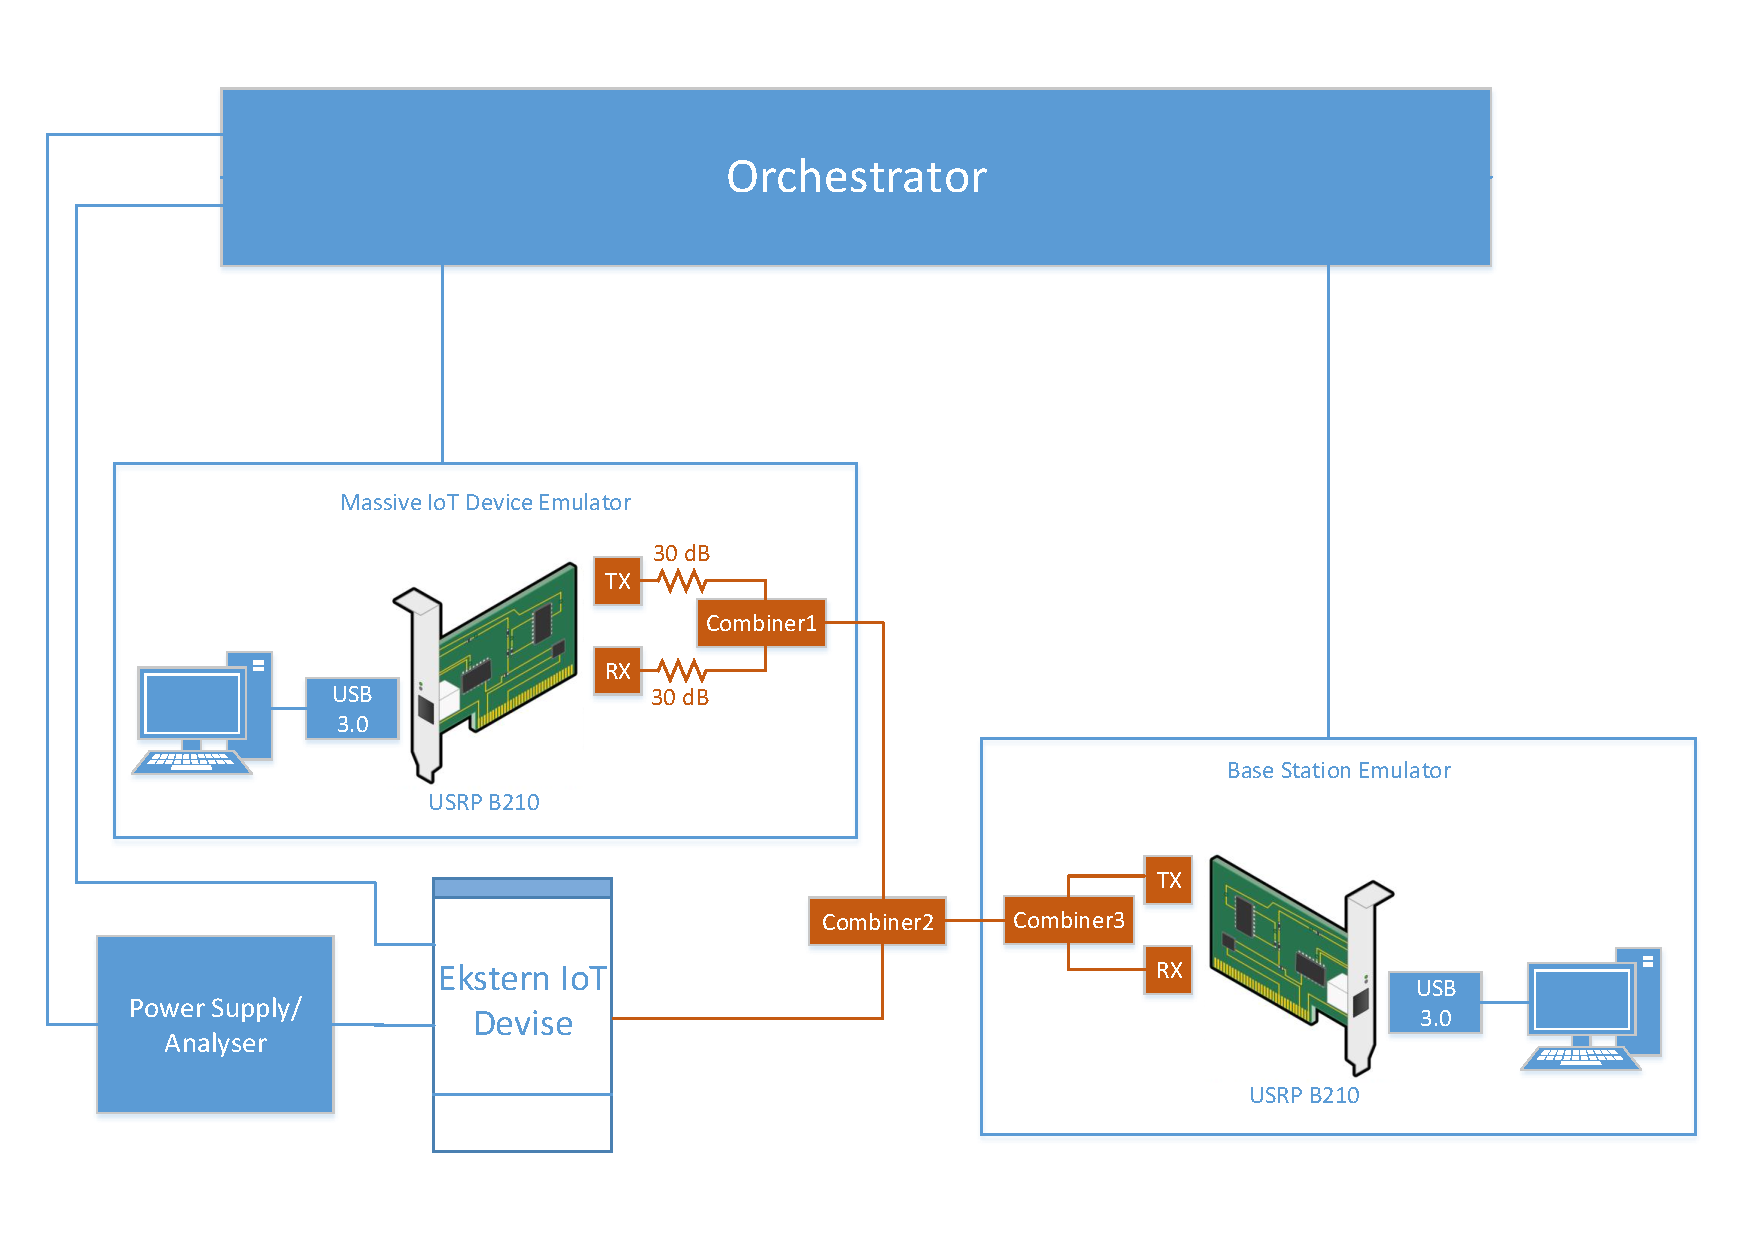
\includegraphics[width=\textwidth]{figures/General_test_setup.pdf}
\caption{A setup which enables testing of all domains on a single device through the massive device emulation.}
\label{fig:Fsetup}
\end{figure}


The setup contains the MDE for the massiveness domain, which will produce interference, both at a signalling level and sharing resources at different layers of the protocol. The PSU will provide power and analyse the power consumption for the DUT. The only domain not tested in this project is the reliability, this could be tested through logging of retransmissions. For this part emulation of different channel conditions for the DUT is very important, as reliability is severely effected by the channel. This is thought to be enough to measure each domain, as other parameters that effect the reliability are already built into the system, like the different cell parameters from the NB-IoT protocol.




%% literaturliste og bilag %%
\bookmarksetup{startatroot}% this is it
\addtocontents{toc}{\bigskip}% perhaps as well
\bibliography{setup/mybib}
\label{bib:mybiblio}
 
 \newpage
 \fancyhead[RO]{\small Appendix \nouppercase\rightmark} %even page - chapter title
 \fancyhead[LE]{\small Appendix \nouppercase\rightmark} %uneven page - section title
\fancyhead[RE,LO]{}
 \titleformat{\section}[hang]{\Large\bfseries}{\thesection\hsp\textcolor{black}{|}\hsp}{0pt}{\Large\bfseries}

 \renewcommand{\thesection}{\Alph{section}}
 \setcounter{section}{0}




\chapter*{Appendix}
 \addcontentsline{toc}{chapter}{Appendix}
 \addtocounter{chapter}{1}
% \section{Battery Consumption Model}
\label{app:bat_model}
(Should be limited to only 1 device in the network)

\begin{equation}
L(t_i) = \frac{C_{bat}\cdot SF_{bat}}{P_m(t_i) + P_{device}}
\end{equation}
\begin{where}
\va{$L(t_i)$}{is the expected lifetime of the battery}{h}
\va{$t_i$}{is the transmission time interval}{h}
\va{$C_{bat}$}{is the capacity of the battery}{Wh}
\va{$SF_{bat}$}{is the safety factor of the battery}{1}
\va{$P_m(t_i)$}{is the power consumption of the modem}{W}
\va{$P_{device}$}{is the power consumption of the IoT device}{W}
\end{where}

\textbf{Battery capacity}\\
This is set from the requirements to 5 Wh

\textbf{Battery safety factor}\\
set to 0.5 in paper we probably can not use

\textbf{Device power consumption}\\
Modem off on the used devices. It is a little irrelevant as none of the devices are final and low power. Should still be measured to draw some conclusion anyway, might be negligible.

\textbf{Modem power consumption}\\

\begin{equation}
P_m(t_i) = \frac{E_{conn} + E_{tx} + E_{disconn} + E_{idle}}{t_i}
\end{equation}
\begin{where}
\va{$E_{conn}$}{is the energy used to connect to the network}{J}
\va{$E_{tx}$}{is the energy used during transmission}{J}
%\va{$t_{tx}$}{is the time it takes to transmit}{s}
\va{$E_{disconn}$}{is the energy used to disconnect from the network}{J}
\va{$E_{idle}$}{is the energy used during the idle period}{J}
%\va{$t_{conn}$}{is the time it takes to connect to the network}{s}
%\va{$t_{disconn}$}{is the time it takes to disconnect from the network}{s}
\end{where}

\textbf{Energy used to Connect to the Network}

\begin{equation}
E_{conn} = E_{modem,on} + E_{sync} + E_{attach}
\end{equation}

$E_{modem,on}$\\
parameters: modem\\
The energy to turn the modem on.

$E_{sync}$\\
parameters: modem, frequency, operation mode, coverage level\\
The energy to synchronize to the network.

$E_{attach}$\\
parameters: modem, frequency, path loss, operation mode, coverage level\\
The energy to attach to the network. Should be split so that attachment from different idle states is supported (with and without AS).

\textbf{Transmission Power}
\begin{equation}
E_{tx} = P_{tx}\cdot t_{tx}
\end{equation}

$P_{tx}$\\
parameters: modem, frequency, path loss\\
Transmission power

$t_{tx}$\\
parameters: operation mode, coverage level, amount of data\\
Transmission time

\textbf{Disconnection Energy}
Overhead of detach procedure

\textbf{Idle Mode Power}
\begin{equation}
E_{idle} = P_{eDRX}\cdot t_{eDRX}+P_{PSM}\cdot t_{PSM}
\end{equation}

$P_{eDRX,PSM}$\\
parameters: modem, paging interval\\
Power consumed in idle modes

$t_{eDRX,PSM}$\\
parameters: timer settings\\
Time spent in eDRX and PSM mode respectively.









 \section{Amarisoft LTE 100 Base Station Emulator}
\label{app:Amarisoft}

 \section{Test Procedures for Battery Lifetime Estimation Tests}
\label{app:test_procedures}

\subsection{Test Procedure for Attach and Release Test Case}
\begin{enumerate}
\item Setup the \gls{DUT} as shown on \autoref{fig:IPE_test_setup}
\item Turn on power supply 
\item Input settings as described in \autoref{tab:setup_parameters}
\item Input chosen value of chosen parameter
\item Put device in disconnected state 
\item Input to log "start <Parameters used> <Parameter value>"
\item Turn on power analyser
\item Start up and attach of DUT
\item Verify connection to cell
\item Release DUT
\item Turn off power analyser
\item Save L3 log from UXM as "Attach\_<Parameters used>\_<Parameters value>.xml"
\item Turn off power supply
\item Change to next value
\item Repeat step 4-14 for all values
\item Save measurements as "Attach\_<Parameters used>\_MessageLog.csv"
\item Change to next parameter
\item Repeat step 3-17 for all parameters
\item Turn off power supply
\end{enumerate}

\subsection{Test Procedure for Transmit Test Case}
\begin{enumerate}
\item Setup the \gls{DUT} as shown on \autoref{fig:IPE_test_setup}
\item Turn on power supply 
\item Put in settings as described in \autoref{tab:setup_parameters} 
\item Enable MAC padding in UL and DL
\item Input chosen value of chosen parameter
\item Input to log "start <Parameter used> <Parameter value>"
\item Put device in connected state
\item Measure power output over 35 s
\item Disconnect device
\item Change to next value
\item Repeat step 5-10 for all values.
\item Save measurements as "Transmit/<Parameter used>/Messagelog.csv"
\item Change to next parameter
\item Repeat step 5-13 for all parameters.
\item Turn off power supply
\end{enumerate}

\subsection{Test Procedure for Idle Test Case}
\begin{enumerate}
\item Setup the \gls{DUT} as shown on \autoref{fig:IPE_test_setup}
\item Turn on power supply 
\item Put in settings as described in \autoref{tab:setup_parameters}
\item Start to measure power output
\item Connect device to cell
\item Release device from cell
\item Wait for measurements to stop
\item Save measurements as "Idle/DRX.csv"
\item Set Idle mode eDRX state to On
\item Repeat step 5-8
\item Save measurements as "Idle/eDRX.csv"
\item Set Idle mode eDRX state to Off and PSM On
\item Repeat step 5-8
\item Save measurements as "Idle/PSM.csv"
\end{enumerate}
 \section{Config file for SRS code}
\label{app:SRSconfig}

\#\#\#\#\#\#\#\#\#\#\#\#\#\#\#\#\#\#\#\#  \\
\#                   srsUE configuration file  \\
\#\#\#\#\#\#\#\#\#\#\#\#\#\#\#\#\#\#\#\#  \\
\# RF configuration  \\
\#  \\
\# dl\_earfcn: Downlink EARFCN code.  \\
\# freq\_offset: Uplink and Downlink optional frequency offset (in Hz)  \\
\# tx\_gain: Transmit gain (dB).   \\
\# rx\_gain: Optional receive gain (dB). If disabled, AGC if enabled  \\
\#  \\
\# Optional parameters:   \\
\# nof\_rx\_ant:         Number of RX antennas (Default 1, supported 1 or 2)  \\
\# device\_name:        Device driver family. Supported options: "auto" (uses first found), "UHD" or "bladeRF" \\  
\# device\_args:        Arguments for the device driver. Options are "auto" or any string.   \\
\#                     Default for UHD: "recv\_frame\_size=9232,send\_frame\_size=9232"  \\
\#                     Default for bladeRF: ""  \\
\# \#time\_adv\_nsamples: Transmission time advance (in number of samples) to compensate for RF delay   \\
\#                     from antenna to timestamp insertion.   \\
\#                     Default "auto". B210 USRP: 100 samples, bladeRF: 27.  \\
\# burst\_preamble\_us:  Preamble length to transmit before start of burst.   \\
\#                     Default "auto". B210 USRP: 400 us, bladeRF: 0 us.   \\
\#\#\#\#\#\#\#\#\#\#\#\#\#\#\#\#\#\#\#\#  \\

$[$rf$]$  \\
\# 759.6 MHz  \\
dl\_earfcn = 6310  \\
\# 801.3 MHz  \\
\#dl\_earfcn = 6253  \\
freq\_offset = 0  \\
tx\_gain = 40  \\
rx\_gain = 40  \\
  \\
\#nof\_rx\_ant = 1  \\
\#device\_name = auto  \\
\#device\_args = auto  \\
\#time\_adv\_nsamples = auto  \\
time\_adv\_nsamples = 65  \\
\#burst\_preamble\_us = auto  \\
  
  
\#\#\#\#\#\#\#\#\#\#\#\#\#\#\#\#\#\#\#\#  \\
\# MAC-layer packet capture configuration  \\
\#  \\
\# Packets are captured to file in the compact format decoded by   \\
\# the Wireshark mac-lte-framed dissector and with DLT 147.   \\
\# To use the dissector, edit the preferences for DLT\_USER to   \\
\# add an entry with DLT=147, Payload Protocol=mac-lte-framed.  \\
\# For more information see: https://wiki.wireshark.org/MAC-LTE  \\
\#  \\
\# enable:   Enable MAC layer packet captures (true/false)  \\
\# filename: File path to use for packet captures  \\
\#\#\#\#\#\#\#\#\#\#\#\#\#\#\#\#\#\#\#\#  \\

$[$pcap$]$  \\
enable = false  \\
filename = /tmp/ue.pcap  \\
  
\#\#\#\#\#\#\#\#\#\#\#\#\#\#\#\#\#\#\#\#  \\
\# Log configuration  \\
\#  \\
\# Log levels can be set for individual layers. "all\_level" sets log  \\
\# level for all layers unless otherwise configured.  \\
\# Format: e.g. phy\_level = info  \\
\#  \\
\# In the same way, packet hex dumps can be limited for each level.  \\
\# "all\_hex\_limit" sets the hex limit for all layers unless otherwise  \\
\# configured.  \\
\# Format: e.g. phy\_hex\_limit = 32  \\
\#  \\
\# Logging layers: phy, mac, rlc, pdcp, rrc, nas, gw, usim, all  \\
\# Logging levels: debug, info, warning, error, none  \\
\#  \\
\# filename: File path to use for log output  \\
\#\#\#\#\#\#\#\#\#\#\#\#\#\#\#\#\#\#\#\#  \\

$[$log$]$  \\
all\_level = warning  \\
all\_hex\_limit = 32  \\
\#filename = /tmp/ue.log  \\
filename = stdout  \\
  
\#\#\#\#\#\#\#\#\#\#\#\#\#\#\#\#\#\#\#\#  \\
\# USIM configuration  \\
\#  \\
\# algo: Authentication algorithm (xor/milenage)  \\
\# op:   128-bit Operator Variant Algorithm Configuration Field (hex)  \\
\# amf:  16-bit Authentication Management Field (hex)  \\
\# k:    128-bit subscriber key (hex)  \\
\# imsi: 15 digit International Mobile Subscriber Identity  \\
\# imei: 15 digit International Mobile Station Equipment Identity  \\
\#\#\#\#\#\#\#\#\#\#\#\#\#\#\#\#\#\#\#\#  \\

$[$usim$]$  \\
algo = xor  \\
op   = 63BFA50EE6523365FF14C1F45F88737D  \\
amf  = 9001  \\
k    = 00112233445566778899aabbccddeeff  \\
imsi = 001010123456789  \\
imei = 353490069873319  \\
  
$[$gui$]$  \\
enable = false  \\
  
\#\#\#\#\#\#\#\#\#\#\#\#\#\#\#\#\#\#\#\#  \\
\# Expert configuration options  \\
\#  \\
\# ue\_category:          Sets UE category (range 1-5). Default: 4   \\
\#  \\
\# prach\_gain:           PRACH gain (dB). If defined, forces a gain for the tranmsission of PRACH only.,   \\
\#                       Default is to use tx\_gain in $[$rf$]$ section.   \\
\# cqi\_max:              Upper bound on the maximum CQI to be reported. Default 15.   \\
\# cqi\_fixed:            Fixes the reported CQI to a constant value. Default disabled.  \\
\# snr\_ema\_coeff:        Sets the SNR exponential moving average coefficient (Default 0.1)  \\
\# snr\_estim\_alg:        Sets the noise estimation algorithm. (Default refs)  \\
\#                          Options: pss:   use difference between received and known pss signal,   \\
\#                                   refs:  use difference between noise references and noiseless (after filtering) \\  
\#                                   empty: use empty subcarriers in the boarder of pss/sss signal  \\
\# pdsch\_max\_its:        Maximum number of turbo decoder iterations (Default 4)  \\
\# attach\_enable\_64qam:  Enables PUSCH 64QAM modulation before attachment (Necessary for old   \\
\#                        Amarisoft LTE 100 eNodeB, disabled by default)  \\
\# nof\_phy\_threads:      Selects the number of PHY threads (maximum 4, minimum 1, default 2)  \\
\# equalizer\_mode:       Selects equalizer mode. Valid modes are: "mmse", "zf" or any   \\
\#                       non-negative real number to indicate a regularized zf coefficient.  \\
\#                       Default is MMSE.   \\
\# cfo\_integer\_enabled:  Enables integer CFO estimation and correction. This needs improvement \\ 
\#                       and may lead to incorrect synchronization. Use with caution.   \\
\# cfo\_correct\_tol\_hz:   Tolerance (in Hz) for digial CFO compensation. Lower tolerance means that   \\
\#                       a new table will be generated more often.   \\
\# time\_correct\_period:  Period for sampling time offset correction. Default is 10 (ue\_sync.c),   \\
\#                       good for long channels. For best performance at highest SNR reduce it to 1.  \\  
\# sfo\_correct\_disable:  Disables phase correction before channel estimation to compensate for   \\
\#                       sampling frequency offset. Default is enabled.   \\
\# sss\_algorithm:        Selects the SSS estimation algorithm. Can choose between   \\
\#                       {full, partial, diff}.   \\
\# estimator\_fil\_w:      Chooses the coefficients for the 3-tap channel estimator centered filter.  \\ 
\#                       The taps are $[$w, 1-2w, w$]$  \\
\# metrics\_period\_secs:  Sets the period at which metrics are requested from the UE.   \\
\#  \\
\# pregenerate\_signals:  Pregenerate uplink signals after attach. Improves CPU performance.  \\
\#  \\
\#\#\#\#\#\#\#\#\#\#\#\#\#\#\#\#\#\#\#\#  \\

$[$expert$]$  \\
phy.verbose          = error  \\
\#n\_id\_ncell           = 37  \\
nbiot\_r14            = false  \\
ue\_category          = nb1  \\
\#n\_id\_ncell           = 0  \\
prach\_gain          = 20  \\
\#cqi\_max             = 15  \\
\#cqi\_fixed           = 10  \\
\#snr\_ema\_coeff       = 0.1  \\
\#snr\_estim\_alg       = refs  \\
\#pdsch\_max\_its       = 4  \\
\#attach\_enable\_64qam = false\\  
nof\_phy\_threads     = 1  \\
\#equalizer\_mode      = mmse\\  
\#cfo\_integer\_enabled = false\\  
\#cfo\_correct\_tol\_hz  = 50  \\
\#cfo\_pss\_ema	     = 0.1  \\
cfo\_ema		     = 0.1  \\
time\_correct\_period = 0  \\
\#sfo\_correct\_disable = false \\ 
\#sss\_algorithm       = full  \\
\#estimator\_fil\_w     = 0.1  \\
\#pregenerate\_signals = false  \\
\#metrics\_csv\_enable = true  \\
\#metrics\_csv\_filename = /tmp/ue\_metrics.csv  \\
  
\#\#\#\#\#\#\#\#\#\#\#\#\#\#\#\#\#\#\#\#  \\
\# Manual RF calibration  \\
\#  \\
\# Applies DC offset and IQ imbalance to TX and RX modules.   \\
\# Currently this configuration is only used if the detected device is a bladeRF  \\
\#  \\
\# tx\_corr\_dc\_gain: TX DC offset gain correction  \\
\# tx\_corr\_dc\_phase: TX DC offset phase correction  \\
\# tx\_corr\_iq\_i: TX IQ imbalance inphase correction  \\
\# tx\_corr\_iq\_q: TX IQ imbalance quadrature correction \\ 
\# same can be configured for rx\_*  \\
\#\#\#\#\#\#\#\#\#\#\#\#\#\#\#\#\#\#\#\# \\  

$[$rf\_calibration$]$  \\
tx\_corr\_dc\_gain = 20  \\
tx\_corr\_dc\_phase = 184  \\
tx\_corr\_iq\_i = 19  \\
tx\_corr\_iq\_q = 97  \\
  
$[$mass$]$  \\
number\_of\_ue = 12 \\
 \section{UXM full configuration list}
%\begin{table}

\begin{longtable}{|p{8cm}|p{5cm}|} \hline
\textbf{Parameter}                                      & \textbf{Value}     \\ \hline
Aggregatoin Level USS                                   & N2                 \\ \hline
Alpha                                                   & AL1                \\ \hline
Candidate Index in USS with Aggr. Level 1               & 0                  \\ \hline
Cell ID                                                 & 0                  \\ \hline
Cell type                                               & NB-IoT             \\ \hline
CP format                                               & Normal             \\ \hline
DCI format                                              & DCI3               \\ \hline
DCI Repetition Index                                    & 1                  \\ \hline
DL Allocation                                           & On                 \\ \hline
DL MCS                                                  & 4                  \\ \hline
DL Off Duration                                         & 0                  \\ \hline
DL  Scheduling Delay Index                              & 1                  \\ \hline
DRX Start Offset                                        & 0                  \\ \hline
drx-ULRetransmissionTimer                               & 0                  \\ \hline
Enable-p0-UE-PUSCH(RBC)                                 & off                \\ \hline
HARQ-ACK Ressource Index                                & 0                  \\ \hline
Host cell DL\_EARFCN                                    & 6240               \\ \hline
Idle eDRX Cycle                                         & 20480 subframes    \\ \hline
Idle eDRX State                                         & Off                \\ \hline
Inactivity Timer                                        & 8 NPDCCH subframes \\ \hline
Long DRX cycle                                          & 1024 subframes     \\ \hline
MAC padding DL                                          & off                \\ \hline
Max Number of Preamble Transmission per PRACH Ressource & N6                 \\ \hline
Max Repetition NPDCCH                                   & 4                  \\ \hline
Number of cells                                         & 1                  \\ \hline
Number of Subcarriers                                   & N12                \\ \hline
Number of tones                                         & N1                 \\ \hline
onDuration Timer                                        & 4 NPDCCH subframes \\ \hline
Operation mode                                          & Standalone         \\ \hline
P0\_UE-PUSCH(RBC)                                       & 0 dB               \\ \hline
p0-NominalPUSCH                                         & -65 dBm            \\ \hline
p0-UE-PUSCH(SRB)                                        & 0 dB               \\ \hline
PDCCH Offset in CSS                                     & V0                 \\ \hline
PDCCH Offset in USS                                     & V0                 \\ \hline
Periodicity                                             & MS40               \\ \hline
Power Saving Mode                                       & Off                \\ \hline
PRB offset                                              & 0                  \\ \hline
pSRS-Offset                                             & 3                  \\ \hline
PTW                              						& 5120 subframes     \\ \hline
$P_{TX}$                                                & 23 dBm             \\ \hline
Reference Signal SIB2                                   & 18                 \\ \hline
Rep CSS for Paging                                      & R8                 \\ \hline
Rep CSS for RA                                          & R64                \\ \hline
Repetition NPDSCH                                       & 1                  \\ \hline
Repetition NPRACH                                       & 1                  \\ \hline
Repetition NPUSCH                                       & 1                  \\ \hline
Repetition USS                                          & R4                 \\ \hline
Retransmission Timer                                    & 2 NPDCCH subframes \\ \hline
RSRP Threshold Count                                    & 0                  \\ \hline
RSRP Threshold Level 1                                  & 55                 \\ \hline
RSRP Threshold Level 2                                  & 30                 \\ \hline
RU Index ALL UL                                         & 6                  \\ \hline
Spacing                                                 & KHZ15              \\ \hline
Spectrum Emission                                       & 1                  \\ \hline
Start Subframe CSS                                      & V2                 \\ \hline
Start Subframe USS                                      & V2                 \\ \hline
Start Time                                              & MS8                \\ \hline
Subcarrier Msg3 Range Start                             & ONEThird           \\ \hline
Subcarrier Offset                                       & N12                \\ \hline
Subframe Index                                          & 6                  \\ \hline
T3324 (DRX period)                                      & 10 s               \\ \hline
T3412 (PSM period)                                      & 10 s               \\ \hline
Tx power                                                & -80 dB/per 15 kHz  \\ \hline
UL Allocation Status                                    & On                 \\ \hline
UL MCS                                                  & 4                  \\ \hline
UL Off Duration                                         & 0                  \\ \hline
UL Position                                             & 0                  \\ \hline
UL Scheduling Delay Index                               & 0                  \\ \hline
\end{longtable}
%\end{table}




\end{document}